%This file is just a wrapper. Please, edit the files for your chapter in chapters/chapter1/.
%Don't worry, we will put your chapter in the correct place when assemble the book.

\documentclass[8pt,a4paper]{book}
\usepackage{classicthesis}
\usepackage[T1]{fontenc}
\usepackage{newpxtext,newpxmath}
%\usepackage{fontspec}
\usepackage{fontawesome}
\usepackage{fixltx2e,fix-cm}
\usepackage{amssymb}
\usepackage{amsmath}
\usepackage{graphicx}
\usepackage{listings,inconsolata}
\usepackage{fbb}


\usepackage{xcolor}
\definecolor{commentgreen}{RGB}{2,112,10}
\definecolor{eminence}{RGB}{108,48,130}
\definecolor{weborange}{RGB}{255,165,0}
\definecolor{frenchplum}{RGB}{129,20,83}

\usepackage{amsmath}  % for \hookrightarrow
\lstset{
 language=caml,
 columns=[c]fixed,
 basicstyle=\small\ttfamily,
 keywordstyle=\bfseries,
 upquote=true,
 commentstyle=,
 breaklines=true,
  postbreak=\mbox{\textcolor{red}{$\hookrightarrow$}\space},
 showstringspaces=false,
    commentstyle=\color{commentgreen},
    keywordstyle=\color{eminence},
    stringstyle=\color{red},
 stringstyle=\color{blue},
emphstyle={\color{blue}},
    keywordstyle=\color{weborange},
 literate={'"'}{\textquotesingle "\textquotesingle}3,
numbers=left,
    numberstyle=\footnotesize,
frame=single,
    xleftmargin=5pt,
    xrightmargin=3pt,
    aboveskip = 20pt,
    rulecolor=\color{black}
}
\makeatletter
\lstdefinelanguage{llvm}{
  morecomment = [l]{;},
  morestring=[b]", 
  sensitive = true,
  classoffset=0,
  morekeywords={
    define, declare, global, constant,
    internal, external, private,
    linkonce, linkonce_odr, weak, weak_odr, appending,
    common, extern_weak,
    thread_local, dllimport, dllexport,
    hidden, protected, default,
    except, deplibs,
    volatile, fastcc, coldcc, cc, ccc,
    x86_stdcallcc, x86_fastcallcc,
    ptx_kernel, ptx_device,
    signext, zeroext, inreg, sret, nounwind, noreturn,
    nocapture, byval, nest, readnone, readonly, noalias, uwtable,
    inlinehint, noinline, alwaysinline, optsize, ssp, sspreq,
    noredzone, noimplicitfloat, naked, alignstack,
    module, asm, align, tail, to,
    addrspace, section, alias, sideeffect, c, gc,
    target, datalayout, triple,
    blockaddress
  },
  classoffset=1, keywordstyle=\color{purple},
  morekeywords={
    fadd, sub, fsub, mul, fmul,
    sdiv, udiv, fdiv, srem, urem, frem,
    and, or, xor,
    icmp, fcmp,
    eq, ne, ugt, uge, ult, ule, sgt, sge, slt, sle,
    oeq, ogt, oge, olt, ole, one, ord, ueq, ugt, uge,
    ult, ule, une, uno,
    nuw, nsw, exact, inbounds,
    phi, call, select, shl, lshr, ashr, va_arg,
    trunc, zext, sext,
    fptrunc, fpext, fptoui, fptosi, uitofp, sitofp,
    ptrtoint, inttoptr, bitcast,
    ret, br, indirectbr, switch, invoke, unwind, unreachable,
    malloc, alloca, free, load, store, getelementptr,
    extractelement, insertelement, shufflevector,
    extractvalue, insertvalue,
  },
  alsoletter={\%},
  keywordsprefix={\%},
}
\makeatother
\usepackage{subfigure}
\usepackage{makeidx}
\usepackage{multicol}
\usepackage[pdfstartview=FitH]{hyperref}
%\usepackage{bookmark}
%\usepackage[dvips]{hyperref}
%% Pandoc tightlist

\providecommand{\tightlist}{%
  \setlength{\itemsep}{0pt}\setlength{\parskip}{0pt}}
\usepackage{relsize}
\frenchspacing
\tolerance=5000

\makeindex
\newcommand{\ignoresecond}[2]{#1}
%\newtheorem{theorem}{Theorem}
\newtheorem{exercise}{Exercise}[chapter]
\newtheorem{example}{Example}
\newtheorem{definition}{Definition}
\newtheorem{proof}{Proof}
 %place custom commands and macros here

\begin{document}

\frontmatter

\title{Creating the Bolt Compiler
%in Socio-Environmental Systems, Public Health, and Insurance\\
%{\Large(Applied Environmental Statistics Series)}
}
\author{Mukul Rathi}

\maketitle

%\cleardoublepage
\thispagestyle{empty}
\vspace*{\stretch{1}}
\begin{center}
\Large\itshape
To my dog\\
and my cat.
\end{center}
\vspace{\stretch{2}}
\cleardoublepage
%\setcounter{page}{7} %previous pages will be reserved for frontmatter to be added in later.
\tableofcontents
%\chapter*{Foreword}
I am delighted to introduce the first book on Multimedia Data Mining.  When I came to know about this book project undertaken by two of the most active young researchers in the field, I was pleased that this book is coming in early stage of a field that will need it more than most fields do.  In most emerging research fields, a book can play a significant role in bringing some maturity to the field.  Research fields advance through research papers.  In research papers, however, only a limited perspective could be provided about the field, its application potential, and the techniques required and already developed in the field.  A book gives such a chance.  I liked the idea that there will be a book that will try to unify the field by bringing in disparate topics already available in several papers that are not easy to find and understand.  I was supportive of this book project even before I had seen any material on it.  The project was a brilliant and a bold idea by two active researchers.  Now that I have it on my screen, it appears to be even a better idea.  

Multimedia started gaining recognition in 1990s as a field.  Processing, storage, communication, and capture and display technologies had advanced enough that researchers and technologists started building approaches to combine information in multiple types of signals such as audio, images, video, and  text.  Multimedia computing and communication techniques recognize correlated information in multiple sources as well as insufficiency of information in any individual source.    By properly selecting sources to provide complementary information, such systems aspire, much like human perception system, to create a holistic picture of a situation using only partial information from separate sources.

Data mining is a direct outgrowth of progress in data storage and processing speeds.  When it became possible to store large volume of data and run different statistical computations to explore all possible and even unlikely correlations among data, the field of data mining was born.  Data mining allowed people to hypothesize relationships among data entities and explore support for those.  This field has been put to applications in many diverse domains and keeps getting more applications.  In fact many new fields are direct outgrowth of data mining and it is likely to become a powerful computational tool.\vadjust{\vfill\pagebreak}



%\chapter*{Preface}
Approximately 17 million people in the USA (6{\%} of the
population) and 140 million people worldwide (this number is
expected to rise to almost 300 million by the year 2025) suffer
from \textit{diabetes mellitus}. Currently, there a few dozens of
commercialised devices for detecting blood glucose levels [1].
However, most of them are invasive. The development of a
noninvasive method would considerably improve the quality of life
for diabetic patients, facilitate their compliance for glucose
monitoring, and reduce complications and mortality associated with
this disease. Noninvasive and continuous monitoring of glucose
concentration in blood and tissues is one of the most challenging
and exciting applications of optics in medicine. The major
difficulty in development and clinical application of optical
noninvasive blood glucose sensors is associated with very low
signal produced by glucose molecules. This results in low
sensitivity and specificity of glucose monitoring by optical
methods and needs a lot of efforts to overcome this difficulty.

A wide range of optical technologies have been designed in
attempts to develop robust noninvasive methods for glucose
sensing. The methods include infrared absorption, near-infrared
scattering, Raman, fluorescent, and thermal gradient
spectroscopies, as well as polarimetric, polarization
heterodyning, photonic crystal, optoacoustic, optothermal, and
optical coherence tomography (OCT) techniques [1-31].

For example, the polarimetric quantification of glucose is based
on the phenomenon of optical rotatory dispersion, whereby a chiral
molecule in an aqueous solution rotates the plane of linearly
polarized light passing through the solution. The angle of
rotation depends linearly on the concentration of the chiral
species, the pathlength through the sample, and the molecule
specific rotation. However, polarization sensitive optical
technique makes it difficult to measure \textit{in vivo} glucose
concentration in blood through the skin because of the strong
light scattering which causes light depolarization. For this
reason, the anterior chamber of the eye has been suggested as a
sight well suited for polarimetric measurements, since scattering
in the eye is generally very low compared to that in other
tissues, and a high correlation exists between the glucose in the
blood and in the aqueous humor. The high accuracy of anterior eye
chamber measurements is also due to the low concentration of
optically active aqueous proteins within the aqueous humor.

On the other hand, the concept of noninvasive blood glucose
sensing using the scattering properties of blood and tissues as an
alternative to spectral absorption and polarization methods for
monitoring of physiological glucose concentrations in diabetic
patients has been under intensive discussion for the last decade.
Many of the considered  effects, such as changing of the size,
refractive index, packing, and aggregation of RBC under glucose
variation, are important for glucose monitoring in diabetic
patients. Indeed, at physiological concentrations of glucose,
ranging from 40 to 400 mg/dl, the role of some of the effects may
be modified, and some other effects, such as glucose penetration
inside the RBC and the followed hemoglobin glycation, may be
important [30-32].

Noninvasive determination of glucose was attempted using light
scattering of skin tissue components measured by a
spatially-resolved diffuse reflectance or NIR fre\-quen\-cy-domain
reflectance techniques. Both approaches are based on change in
glucose concentration, which affects the refractive index mismatch
between the interstitial fluid and tissue fibers, and hence
reduces scattering coefficient. A glucose clamp experiment showed
that reduced scattering coefficient measured in the visible range
qualitatively tracked changes in blood glucose concentration for
the volunteer with diabetes studied.




%\listoffigures
%\listoftables
%%%\twocolumn
\chapter*{Contributors}

\begin{multicols}{2}
\contributor{Michael Aftosmis}{NASA Ames Research Center}{Moffett Field, California}

\contributor{Pratul K. Agarwal}{Oak Ridge National Laboratory}{Oak Ridge, Tennessee}

\contributor{Sadaf R. Alam}{Oak Ridge National Laboratory}{Oak Ridge, Tennessee}

\contributor{Gabrielle Allen}{Louisiana State University}{Baton Rouge, Louisiana}

\contributor{Martin Sandve Aln{\ae}s}{Simula Research Laboratory and University of Oslo, Norway}{Norway}

\contributor{Steven F. Ashby} {Lawrence Livermore National Laboratory}{Livermore, California}

\contributor{David A. Bader} {Georgia Institute of Technology}{Atlanta, Georgia}

\contributor{Benjamin Bergen} {Los Alamos National Laboratory}{Los Alamos, New Mexico}

\contributor{Jonathan W. Berry} {Sandia National Laboratories}{Albuquerque, New Mexico}

\contributor{Martin Berzins}{University of Utah}{Salt Lake City, Utah}

\contributor{Abhinav Bhatele}{University of Illinois}{Urbana-Champaign, Illinois}

\contributor{Christian Bischof} {RWTH Aachen University}{Germany}

\contributor{Rupak Biswas} {NASA Ames Research Center}{Moffett Field, California}\vspace*{5pt}

\contributor{Eric Bohm} {University of Illinois}{Urbana-Champaign, Illinois}\vspace*{5pt}

\contributor{James Bordner} {University of California, San Diego}{San Diego, California}\vspace*{5pt}

\contributor{George Bosilca} {University of Tennessee}{Knoxville, Tennessee}\vspace*{5pt}

\contributor{Greg L. Bryan} {Columbia University}{New York, New York}\vspace*{5pt}

\contributor{Marian Bubak} {AGH University of Science and Technology}{
Krak{\'o}w, Poland}\vspace*{5pt}

\contributor{Andrew Canning}{Lawrence Berkeley National
Laboratory}{Berkeley, California}

\contributor{Jonathan Carter} {Lawrence Berkeley National
Laboratory}{Berkeley, California}

\contributor{Zizhong Chen} {Jacksonville State University}{Jacksonville,
Alabama}

\contributor{Joseph R. Crobak} {Rutgers, The State University of New
Jersey}{Piscataway, New Jersey}

\contributor{Roxana E. Diaconescu} {Yahoo! Inc.}{Burbank, California}

\contributor{Peter Diener}
{Louisiana State University}{Baton Rouge, Louisiana}

\contributor{Jack J. Dongarra} {University of Tennessee, Knoxville, 
Oak Ridge National Laboratory, and}{University of Manchester}

\contributor{John B. Drake} {Oak Ridge National Laboratory}{Oak Ridge,
Tennessee}

\contributor{Kelvin K. Droegemeier} {University of Oklahoma}{Norman,
Oklahoma}

\contributor{St{\'e}phane Ethier} {Princeton University}{Princeton, New
Jersey}

\contributor{Christoph Freundl}
{Friedrich--Alexander--Universit{\"a}t}{Erlangen, Germany}

\contributor{Karl F{\"u}rlinger} {University of Tennessee}{Knoxville,
Tennessee}

\contributor{Al Geist} {Oak Ridge National Laboratory}{Oak Ridge,
Tennessee}

\contributor{Michael Gerndt} {Technische Universit{\"a}t
M{\"u}nchen}{Munich, Germany}

\contributor{Tom Goodale}
{Louisiana State University}{Baton Rouge, Louisiana}

\contributor{Tobias Gradl}
{Friedrich--Alexander--Universit{\"a}t}{Erlangen, Germany}

\contributor{William D. Gropp} {Argonne National Laboratory}{Argonne,
Illinois}

\contributor{Robert Harkness} {University of California, San
Diego}{San Diego, California}

\contributor{Albert Hartono} {Ohio State University}{Columbus, Ohio}

\contributor{Thomas C. Henderson} {University of Utah}{Salt Lake City,
Utah}

\contributor{Bruce A. Hendrickson} {Sandia National
Laboratories}{Albuquerque, New Mexico}

\contributor{Alfons G. Hoekstra} {University of Amsterdam}{Amsterdam,
The Netherlands}

\contributor{Philip W. Jones} {Los Alamos National Laboratory}{Los
Alamos, New Mexico}

\contributor{Laxmikant Kal{\'e}} {University of
Illinois}{Urbana-Champaign, Illinois}

\contributor{Shoaib Kamil} {Lawrence Berkeley National
Laboratory}{Berkeley, California}

\contributor{Cetin Kiris} {NASA Ames Research Center}{Moffett Field,
California}

\contributor{Uwe K{\"u}ster} {University of Stuttgart}{Stuttgart,
Germany}

\contributor{Julien Langou} {University of Colorado}{Denver, Colorado}

\contributor{Hans Petter Langtangen}
{Simula Research Laboratory and}{University of Oslo, Norway}

\contributor{Michael Lijewski} {Lawrence Berkeley National
Laboratory}{Berkeley, California}

\contributor{Anders Logg}
{Simula Research Laboratory and}{University of Oslo, Norway}

\contributor{Justin Luitjens} {University of Utah}{Salt Lake City, Utah}

\contributor{Kamesh Madduri} {Georgia Institute of Technology}{Atlanta,
Georgia}

\contributor{Kent-Andre Mardal}
{Simula Research Laboratory and}{University of Oslo, Norway}

\contributor{Satoshi Matsuoka} {Tokyo Institute of Technology}{Tokyo,
Japan}

\contributor{John M. May} {Lawrence Livermore National
Laboratory}{Livermore, California}

\contributor{Celso L. Mendes} {University of Illinois}{Urbana-Champaign,
Illinois}

\contributor{Dieter an Mey} {RWTH Aachen University}{Germany}

\contributor{Tetsu Narumi} {Keio University}{Japan}

\contributor{Michael L. Norman} {University of California, San
Diego}{San Diego, California}

\contributor{Boyana Norris} {Argonne National Laboratory}{Argonne,
Illinois}

\contributor{Yousuke Ohno} {Institute of Physical and Chemical Research
(RIKEN)}{Kanagawa, Japan}

\contributor{Leonid Oliker} {Lawrence Berkeley National
Laboratory}{Berkeley, California}

\contributor{Brian O'Shea} {Los Alamos National Laboratory}{Los Alamos,
New Mexico}

\contributor{Christian D. Ott}
{University of Arizona}{Tucson, Arizona}

\contributor{James C. Phillips} {University of
Illinois}{Urbana-Champaign, Illinois}

\contributor{Simon Portegies Zwart} {University of
Amsterdam,}{Amsterdam, The Netherlands}

\contributor{Thomas Radke}
{Albert-Einstein-Institut}{Golm, Germany}

\contributor{Michael Resch} {University of Stuttgart}{Stuttgart,
Germany}

\contributor{Daniel Reynolds} {University of California, San Diego}{San
Diego, California}

\contributor{Ulrich R{\"u}de}
{Friedrich--Alexander--Universit{\"a}t}{Erlangen, Germany}

\contributor{Samuel Sarholz}
{RWTH Aachen University}{Germany}

\contributor{Erik Schnetter}
{Louisiana State University}{Baton Rouge, Louisiana}

\contributor{Klaus Schulten} {University of Illinois}{Urbana-Champaign,
Illinois}

\contributor{Edward Seidel}
{Louisiana State University}{Baton Rouge, Louisiana}

\contributor{John Shalf} {Lawrence Berkeley National
Laboratory}{Berkeley, California}

\contributor{Bo-Wen Shen} {NASA Goddard Space Flight Center}{Greenbelt,
Maryland}

\contributor{Ola Skavhaug}
{Simula Research Laboratory and}{University of Oslo, Norway}

\contributor{Peter M.A. Sloot} {University of Amsterdam}{Amsterdam, The
Netherlands}

\contributor{Erich Strohmaier} {Lawrence Berkeley National
Laboratory}{Berkeley, California}

\contributor{Makoto Taiji} {Institute of Physical and Chemical Research
(RIKEN)}{Kanagawa, Japan}

\contributor{Christian Terboven}
{RWTH Aachen University,}{Germany}

\contributor{Mariana Vertenstein} {National Center for Atmospheric
Research}{Boulder, Colorado}

\contributor{Rick Wagner} {University of California, San Diego}{San
Diego, California}

\contributor{Daniel Weber} {University of Oklahoma}{Norman, Oklahoma}

\contributor{James B. White, III} {Oak Ridge National Laboratory}{Oak
Ridge, Tennessee}

\contributor{Terry Wilmarth} {University of Illinois}{Urbana-Champaign,
Illinois}

\end{multicols}
%\chapter*{Symbols}
\begin{symbollist}{000000}
\symbolentry{$\alpha$}{To solve the generator maintenance scheduling, in the  past, several mathematical techniques have  been applied.}
\symbolentry{$\sigma^2$}{These include integer programming, integer linear programming, dynamic programming, branch and bound etc.}
\symbolentry{$\sum$}{Several heuristic search algorithms have also been developed. In recent years expert systems,}
\symbolentry{$abc$}{fuzzy approaches, simulated annealing and genetic algorithms have also been tested.}
\symbolentry{$\theta\sqrt{abc}$}{This paper presents a survey of the literature}
\symbolentry{$\zeta$}{ over the past fifteen years in the generator}
\symbolentry{$\partial$}{maintenance scheduling. The objective is to}
\symbolentry{sdf}{present a clear picture of the available recent literature}
\symbolentry{ewq}{of the problem, the constraints and the other aspects of}
\symbolentry{bvcn}{the generator maintenance schedule.}
\end{symbollist}

\mainmatter

\part{Introduction}
%\hypertarget{___gatsby}{}
%\hypertarget{gatsby-focus-wrapper}{}
%\href{https://mukulrathi.com/}{}
%
%MUKUL RATHI
%
%\href{https://mukulrathi.com/about-me}{}
%
%About Me
%
%\href{https://mukulrathi.com/blog}{}
%
%Blog

\hypertarget{creating-the-bolt-compiler-part-1}{%
\chapter{Creating the Bolt Compiler: Part
1}\label{creating-the-bolt-compiler-part-1}}

%\hypertarget{top-of-page}{%
%\section{How I wrote my own "proper" programming
%language}\label{top-of-page}}

May 10, 2020 
%\hypertarget{may-10-2020}{%
%\subsection{}\label{may-10-2020}}

%\hypertarget{min-read}{%
%\subsection{7 min read}\label{min-read}}

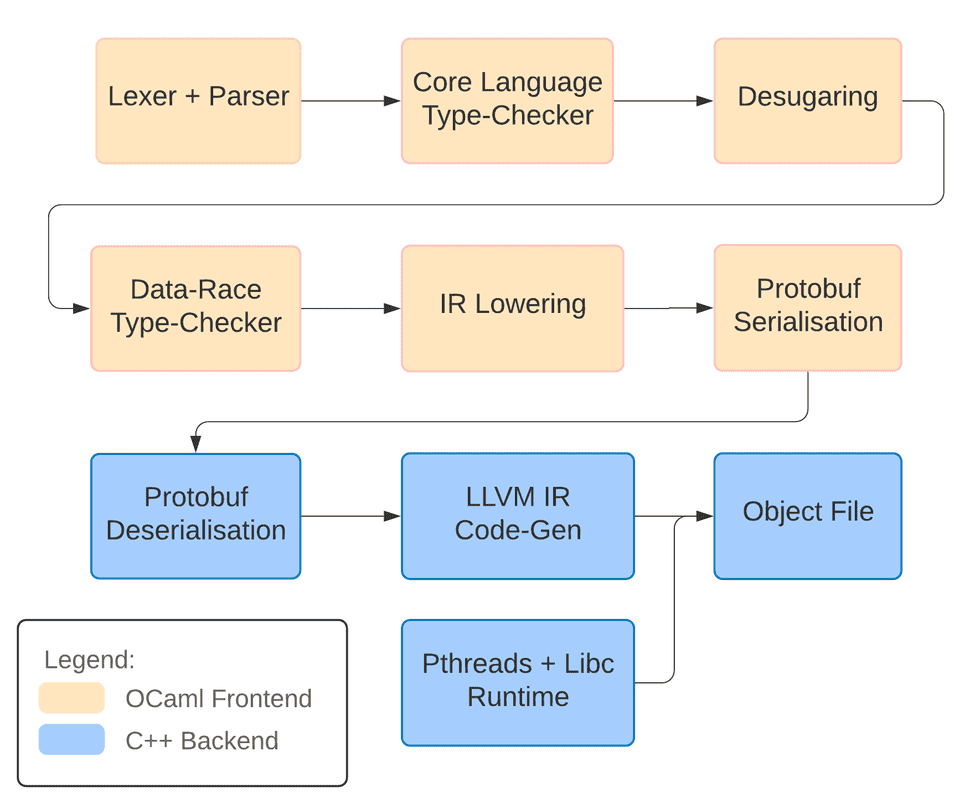
\includegraphics[width=\linewidth]{How I wrote my own proper programming language_files/compiler-pipeline.png}

%
%
%\begin{itemize}
%\item
%  \textbf{Part 1: How I wrote my own "proper" programming language}
%\item
%  { Part 2:
%  }\href{https://mukulrathi.com/create-your-own-programming-language/compiler-engineering-structure/}{So
%  how do you structure a compiler project?}
%\item
%  { Part 3:
%  }\href{https://mukulrathi.com/create-your-own-programming-language/parsing-ocamllex-menhir/}{Writing
%  a Lexer and Parser using OCamllex and Menhir}
%\item
%  { Part 4:
%  }\href{https://mukulrathi.com/create-your-own-programming-language/intro-to-type-checking/}{An
%  accessible introduction to type theory and implementing a
%  type-checker}
%\item
%  { Part 5:
%  }\href{https://mukulrathi.com/create-your-own-programming-language/data-race-dataflow-analysis/}{A
%  tutorial on liveness and alias dataflow analysis}
%\item
%  { Part 6:
%  }\href{https://mukulrathi.com/create-your-own-programming-language/lower-language-constructs-to-llvm/}{Desugaring
%  - taking our high-level language and simplifying it!}
%\item
%  { Part 7:
%  }\href{https://mukulrathi.com/create-your-own-programming-language/protobuf-ocaml-cpp-tutorial/}{A
%  Protobuf tutorial for OCaml and C++}
%\item
%  { Part 8:
%  }\href{https://mukulrathi.com/create-your-own-programming-language/llvm-ir-cpp-api-tutorial/}{A
%  Complete Guide to LLVM for Programming Language Creators}
%\item
%  { Part 9:
%  }\href{https://mukulrathi.com/create-your-own-programming-language/concurrency-runtime-language-tutorial/}{Implementing
%  Concurrency and our Runtime Library}
%\item
%  { Part 10:
%  }\href{https://mukulrathi.com/create-your-own-programming-language/generics-parametric-polymorphism/}{Generics
%  - adding polymorphism to Bolt}
%\item
%  { Part 11:
%  }\href{https://mukulrathi.com/create-your-own-programming-language/inheritance-method-overriding-vtable/}{Adding
%  Inheritance and Method Overriding to Our Language}
%\end{itemize}
%
%\begin{center}\rule{0.5\linewidth}{0.5pt}\end{center}

The diagram above is the compiler for the language Bolt we'll be
building. What do all the stages mean? I have to learn OCaml and C++?
Wait I haven't even heard of OCaml\ldots{}

\textbf{Don't worry.} When I started this project 6 months ago, I had
never built a compiler, nor had I used OCaml or C++ in any serious
project. I'll explain everything in due course.

In this series of posts we'll be building a \emph{proper} programming
language. One of the gripes I had when seeing programming language
tutorials that created a toy language with only operations like addition
and multiplication, was: okay, \emph{but what about a real language like
Java}?

So that's what this series aims to fix. The language Bolt I wrote as
part of my third year disseration is a Java-style concurrent
object-oriented language. Some of the highlights of this series:

\begin{itemize}
\tightlist
\item
  We implement \textbf{objects} and classes, with inheritance and method
  overriding
\item
  \textbf{Concurrency} (as far as I could tell when writing this, no
  other programming language tutorial covered this)
\item
  \textbf{Generics}: being able to write a class of type
  \texttt{LinkedList\textless{}T\textgreater{}} and then instantiating
  it with \texttt{LinkedList\textless{}int\textgreater{}},
  \texttt{LinkedList\textless{}Person\textgreater{}} and so on.
\item
  An introduction to how types are checked in a compiler
\item
  Compiling to LLVM (this post was \#2 on Hacker News!) - LLVM is used
  by C, C++, Swift, Rust amongst many other languages.
\end{itemize}

So I'd encourage you to follow the links in the ``Series'' overview to
learn about these specific features. The remainder of this post will be
to convince you why writing your own programming language is worthwhile,
and the next post will outline the structure of a compiler.

\hypertarget{why-should-you-write-your-own-programming-language}{%
\section{\texorpdfstring{\protect\hyperlink{why-should-you-write-your-own-programming-language}{}Why
should you write your own programming
language?}{Why should you write your own programming language?}}\label{why-should-you-write-your-own-programming-language}}

The question we should really be asking is \emph{why design your own
language}? Possible answers:

\begin{enumerate}
\tightlist
\item
  It's fun
\item
  It's cool to have your own programming language
\item
  It's a good side-project
\end{enumerate}

\hypertarget{mental-models}{%
\section{\texorpdfstring{\protect\hyperlink{mental-models}{}Mental
Models}{Mental Models}}\label{mental-models}}

Whilst all three of these (or none!) might be true, there's a bigger
motivation: having the right \textbf{mental models}. See, when you learn
your first programming language, you view programming through the lens
of that language. Fast forward to your second language, and it seems
hard, you have to relearn syntax and this new language does things
differently. Using more programming languages, you realise that the
languages share common themes. Java and Python have objects, Python and
JavaScript don't require you to write types, the list goes on. Diving
further into programming language theory, you read about the language
constructs present - Java and Python are \emph{object-oriented}
programming languages and Python and JavaScript are
\emph{dynamically-typed}.

The programming languages you've been using actually build upon the
ideas present in older languages that you may not have have heard of.
Simula and Smalltalk introduced the concept of object-oriented
programming languages. Lisp introduced the concept of dynamic typing.
And there are newer research languages coming all the time that
introduce new concepts. A more mainstream example: Rust builds
\textbf{memory-safety} into a low-level systems programming language.

Building your own language (especially if you're adding new ideas) helps
you think more \textbf{critically} about language design, so when you go
learn a new language it's much easier. For example, I had never
programmed in Hack before my internship at Facebook last summer, but
knowing these programming language concepts made it much easier to pick
up.

\hypertarget{what-are-compilers}{%
\section{\texorpdfstring{\protect\hyperlink{what-are-compilers}{}What
are compilers?}{What are compilers?}}\label{what-are-compilers}}

So you've designed your fancy new language and it is going to
revolutionise the world, but there's one problem. \textbf{How do you run
it?} That's the role of a compiler. To explain how compilers work, let's
first flash our minds back to the 19th Century, in the age of the
telegraph. Here we have this fancy new telegraph but how do we send
messages? \textbf{Same problem, different domain.} The telegraph
operator needs to take in speech and convert it to Morse code, and tap
out the code. The first thing the operator does is make sense of the
speech - they split it into words (\textbf{lexing}) , and then
understand how those words are used in a sentence (\textbf{parsing}) -
are they part of a noun phrase, a subordinate clause etc. They check if
it makes sense by classifying words into categories or \textbf{types}
(adjective, noun, verb) and check the sentence makes grammatical sense
(we can't use ``runs'' to describe a noun as it is a verb not a noun).
Finally, they translate (\textbf{compile}) each word into dots and dashs
(Morse code), which is then transmitted along the wire.

This seems like it labours the point, because so much of this is
\emph{automatic} for humans. Compilers work the same way, except we have
to explicitly program computers to do this. The example above describes
a simple compiler consisting of 4 stages: lex, parse, type-check and
then translate into machine instructions. The operator also needs some
additional tools to actually tap out the Morse code; for programming
languages, this is the \textbf{runtime environment}.

In practice, the operator likely constructs some shorthand notation that
they know how to translate to Morse code. Now rather than converting
speech into Morse code directly, they convert the speech into their
shorthand, and then convert the shorthand into Morse code. In many
practical languages, you can't just go directly from the source code to
the machine code, you have \emph{desugaring} or \emph{lowering} stages,
where you remove language constructs stage-by-stage (e.g. unrolling for
loops) until we're left with a small set of instructions that can be
executed. Desugaring makes later stages much easier, as they operate on
a simpler representation. The compiler stages are grouped into frontend,
middle-end and backend, where frontend does much of the
parsing/type-checking, and middle-end and backend simplify and optimise
the code.

\hypertarget{compiler-design-choices}{%
\subsection{\texorpdfstring{\protect\hyperlink{compiler-design-choices}{}Compiler
Design
Choices}{Compiler Design Choices}}\label{compiler-design-choices}}

We can actually frame a lot of language and compiler design in terms of
the analogy above:

Does the operator translate words on-the-fly into Morse code as they
transmit them, or do they convert the words into Morse code beforehand,
and then transmit the Morse code? \textbf{Interpreted} languages like
Python do the former, whilst ahead-of-time \textbf{compiled} languages
like C (and Bolt) do the latter. Java actually lies somewhere in between
- it uses a \textbf{just-in-time} compiler which does most of the work
beforehand, translating programs to bytecode and then at runtime
compiles bytecode to machine code.

Now consider a scenario where a new Lorse code came out that was an
alternative to Morse code. If the operators are taught how to convert
the shorthand to Lorse code, the person speaking doesn't need to know
how that's done, they get it for free. Likewise, a person speaking a
different language just needs to tell the operator how to translate it
to the shorthand, and then they get translations into Lorse \emph{and}
Morse code! This is how \textbf{LLVM} works. \textbf{LLVM IR}
(intermediate representation) acts as the stepping stone that lies
between the program and the machine code. C, C++, Rust and a whole host
of other languages (including Bolt) target LLVM IR, which then compiles
code to a variety of machine architectures.

{
\href{https://mukulrathi.com/static/cf22553f4c173ee4b0dec6bd67e38110/c658e/llvm.png}{{}
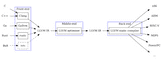
\includegraphics[width=\linewidth]{How I wrote my own proper programming language_files/llvm.png}}
}

Static vs dynamic typing? In the first case, the operator either checks
that the words make grammatical sense before they start tapping. Or,
they don't and then midway through they're like ``huh, this doesn't make
sense'' and stop. Dynamic typing can be seen as quicker to experiment in
(like Python, JS) but when you send that message you don't know if the
operator will stop midway through (crash).

I've explained it in terms of an imaginary telegraph operator, but any
analogy works. Building up this intuition goes a long way in
understanding which language features are right for your language: if
you're going to be experimenting, then maybe dynamic typing is better as
you can move faster. If you're using a larger codebase, it's harder to
proof-read it all and you're more likely to make errors so you probably
should shift towards static typing to avoid breaking things.

\hypertarget{types}{%
\subsection{\texorpdfstring{\protect\hyperlink{types}{}Types}{Types}}\label{types}}

The most interesting part of the compiler (in my opinion) is the
type-checker. In our analogy, the operator classified words as
parts-of-speech (adjectives, nouns, verbs) then checked if they were
used correctly. Types work the same way, we classify program values
based on the behaviour we'd like them to have. E.g. \texttt{int} for
numbers that can be multiplied together, \texttt{String} for streams of
characters that can be concatenated together. The role of the
type-checker is to prevent undesirable behaviour from happening - like
concatenating \texttt{int}s or multiplying \texttt{String}s together -
these operations make no sense so shouldn't be allowed. With type
\emph{checking}, the programmer annotates values with types, and the
compiler checks if they're correct. With type \emph{inference}, the
compiler both infers and checks the types. We call the rules that check
the types \emph{typing judgements}, and a collection of these (along
with the types themselves) forms a type system.

It turns out actually that there's a lot more you can do: type systems
don't just check if \texttt{int}s or \texttt{String}s are used
correctly. Richer type systems can prove stronger invariants about
programs: that they will terminate, access memory safely, or that they
do not contain data races. Rust's type system for example guarantees
memory safety and data-race freedom, as well as checking traditional
types \texttt{int}s and \texttt{String}s.

%\hypertarget{i-make-content-about-my-software-engineering-journey-curated-in-my-newsletter}{%
%\subsection{I make content about my software engineering journey,
%curated in my
%newsletter!}\label{i-make-content-about-my-software-engineering-journey-curated-in-my-newsletter}}
%
%Tips from my time at Cambridge and Facebook, and early access to
%technical tutorials on machine learning, compilers and beyond.
%
%\href{https://newsletter.mukulrathi.com/}{Check out previous issues!}
%
%Email Address
%
%By subscribing, you agree with Revue's
%\href{https://www.getrevue.co/terms}{Terms of Service} and
%\href{https://www.getrevue.co/privacy}{Privacy Policy}.

\hypertarget{where-does-bolt-fit-in}{%
\section{\texorpdfstring{\protect\hyperlink{where-does-bolt-fit-in}{}Where
does Bolt fit
in?}{Where does Bolt fit in?}}\label{where-does-bolt-fit-in}}

Programming languages still haven't cracked the problem of writing safe
concurrent code. Bolt, like Rust, prevents data races
(\href{https://doc.rust-lang.org/nightly/nomicon/races.html}{explained
in this Rust doc}), but takes a more fine-grained approach to
concurrency. Before keyboard warriors come at me on Twitter, I think
Rust has done a brilliant job in getting the conversation about this
going - whilst Bolt will likely never go mainstream, it's demonstrating
another approach.

If we look back at the pipeline now, you can see that Bolt contains the
lexing, parsing, and desugaring/lowering phases. It also contains a
couple of Protobuf serialisation and deserialisation phases: these are
purely to convert between OCaml and C++. It targets LLVM IR, and then we
link in a couple of runtime libraries (pthreads and libc) and finally we
output our \emph{object file}, a binary containing the machine code.

{
\href{https://mukulrathi.com/static/67552b3afe850eb6515a639276f98f47/7792f/compiler-pipeline.png}{{}
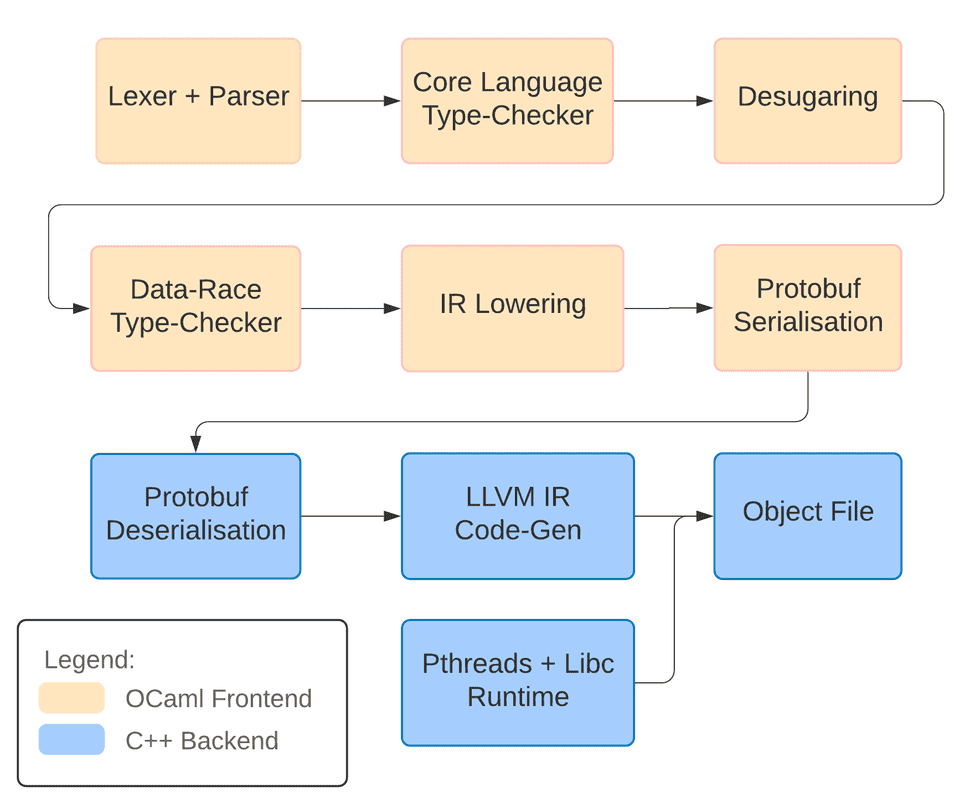
\includegraphics[width=\linewidth]{How I wrote my own proper programming language_files/compiler-pipeline.png}}
}

Unlike most compilers though, Bolt has not one but \textbf{two}
type-checking phases! Bolt has both traditional types and
\textbf{capabilities}, which are, informally, another set of types to
type-check data races. I've
\href{https://github.com/mukul-rathi/bolt-dissertation}{written up a
dissertation} that explores this more formally, if you are interested in
the theory, if not you can skip the data-race checking posts in this
series. We type-check the traditional types first, simplify the language
a bit in the desugaring stage, then do the data-race type-checking.

\hypertarget{and-what-about-this-series}{%
\section{\texorpdfstring{\protect\hyperlink{and-what-about-this-series}{}And
what about this
series?}{And what about this series?}}\label{and-what-about-this-series}}

This series can be thought of from two perspectives: firstly, we will be
discussing language design and comparing Bolt with Java, C++ and other
languages along the way. Secondly, it is a practical step-by-step
tutorial on building your own compiler. Unlike many
build-your-own-compiler tutorials that tell you how to build a
\emph{toy} language, some of the topics this tutorial looks at form the
basis of concurrent object-oriented languages like Java: how classes are
implemented, how inheritance works, generic classes, and even how
concurrency is implemented under the hood.

Bolt also doesn't output toy instructions but instead targets
\textbf{LLVM IR}. Practically speaking, this means Bolt hooks into the
amazing optimisations present in C/C++ compilers. The LLVM API is
powerful, but it's also very hard to navigate the documentation. I spent
many long nights reverse-engineering C++ programs - hopefully this
series prevents at least one person from going through that pain!

In the next part, we'll look at the practical aspects of setting up a
compiler project - I'll walk through the
\href{https://github.com/mukul-rathi/bolt}{Bolt repository} and explain
\emph{why} we're using OCaml of all languages for the frontend.

%\hypertarget{share-this-on-twitter}{%
%\subsection{Share This On Twitter}\label{share-this-on-twitter}}
%
%If you liked this post, please consider sharing it with your network. If
%you have any questions, tweet away and I'll answer :) I also tweet when
%new posts drop!
%
%\textbf{PS:} I also share helpful tips and links as I'm learning - so
%you get them \textbf{well before} they make their way into a post!
%
%\includegraphics[width=1.04167in,height=1.11458in]{How I wrote my own proper programming language_files/profile-pic.png}
%
%\hypertarget{series-creating-the-bolt-compiler-1}{%
%\section{Series: Creating the Bolt
%Compiler}\label{series-creating-the-bolt-compiler-1}}
%
%\begin{itemize}
%\item
%  \textbf{Part 1: How I wrote my own "proper" programming language}
%\item
%  { Part 2:
%  }\href{https://mukulrathi.com/create-your-own-programming-language/compiler-engineering-structure/}{So
%  how do you structure a compiler project?}
%\item
%  { Part 3:
%  }\href{https://mukulrathi.com/create-your-own-programming-language/parsing-ocamllex-menhir/}{Writing
%  a Lexer and Parser using OCamllex and Menhir}
%\item
%  { Part 4:
%  }\href{https://mukulrathi.com/create-your-own-programming-language/intro-to-type-checking/}{An
%  accessible introduction to type theory and implementing a
%  type-checker}
%\item
%  { Part 5:
%  }\href{https://mukulrathi.com/create-your-own-programming-language/data-race-dataflow-analysis/}{A
%  tutorial on liveness and alias dataflow analysis}
%\item
%  { Part 6:
%  }\href{https://mukulrathi.com/create-your-own-programming-language/lower-language-constructs-to-llvm/}{Desugaring
%  - taking our high-level language and simplifying it!}
%\item
%  { Part 7:
%  }\href{https://mukulrathi.com/create-your-own-programming-language/protobuf-ocaml-cpp-tutorial/}{A
%  Protobuf tutorial for OCaml and C++}
%\item
%  { Part 8:
%  }\href{https://mukulrathi.com/create-your-own-programming-language/llvm-ir-cpp-api-tutorial/}{A
%  Complete Guide to LLVM for Programming Language Creators}
%\item
%  { Part 9:
%  }\href{https://mukulrathi.com/create-your-own-programming-language/concurrency-runtime-language-tutorial/}{Implementing
%  Concurrency and our Runtime Library}
%\item
%  { Part 10:
%  }\href{https://mukulrathi.com/create-your-own-programming-language/generics-parametric-polymorphism/}{Generics
%  - adding polymorphism to Bolt}
%\item
%  { Part 11:
%  }\href{https://mukulrathi.com/create-your-own-programming-language/inheritance-method-overriding-vtable/}{Adding
%  Inheritance and Method Overriding to Our Language}
%\end{itemize}
%
%\begin{itemize}
%\item ~
%  \hypertarget{a-step-by-step-guide-to-integrating-reasonml-into-your-gatsby-site}{%
%  \subsection{\texorpdfstring{\href{https://mukulrathi.com/gatsby-reasonml-tutorial/}{←
%  A step-by-step guide to integrating ReasonML into your Gatsby
%  site}}{← A step-by-step guide to integrating ReasonML into your Gatsby site}}\label{a-step-by-step-guide-to-integrating-reasonml-into-your-gatsby-site}}
%\item ~
%  \hypertarget{so-how-do-you-structure-a-compiler-project}{%
%  \subsection{\texorpdfstring{\href{https://mukulrathi.com/create-your-own-programming-language/compiler-engineering-structure/}{So
%  how do you structure a compiler project?
%  →}}{So how do you structure a compiler project? →}}\label{so-how-do-you-structure-a-compiler-project}}
%\end{itemize}
%
%\hypertarget{table-of-contents}{%
%\section{Table of Contents}\label{table-of-contents}}
%
%\href{https://mukulrathi.com/create-your-own-programming-language/intro-to-compiler/\#top-of-page}{}
%
%\hypertarget{how-i-wrote-my-own-proper-programming-language}{%
%\subsection{How I wrote my own "proper" programming
%language}\label{how-i-wrote-my-own-proper-programming-language}}
%
%\begin{itemize}
%\item
%  \href{https://mukulrathi.com/create-your-own-programming-language/intro-to-compiler/\#why-should-you-write-your-own-programming-language}{}
%
%  \hypertarget{why-should-you-write-your-own-programming-language-1}{%
%  \subsection{Why should you write your own programming
%  language?}\label{why-should-you-write-your-own-programming-language-1}}
%\item
%  \href{https://mukulrathi.com/create-your-own-programming-language/intro-to-compiler/\#mental-models}{}
%
%  \hypertarget{mental-models-1}{%
%  \subsection{Mental Models}\label{mental-models-1}}
%\item
%  \href{https://mukulrathi.com/create-your-own-programming-language/intro-to-compiler/\#what-are-compilers}{}
%
%  \hypertarget{what-are-compilers-1}{%
%  \subsection{What are compilers?}\label{what-are-compilers-1}}
%
%  \begin{itemize}
%  \item
%    \href{https://mukulrathi.com/create-your-own-programming-language/intro-to-compiler/\#compiler-design-choices}{}
%
%    \hypertarget{compiler-design-choices-1}{%
%    \subsection{Compiler Design
%    Choices}\label{compiler-design-choices-1}}
%  \item
%    \href{https://mukulrathi.com/create-your-own-programming-language/intro-to-compiler/\#types}{}
%
%    \hypertarget{types-1}{%
%    \subsection{Types}\label{types-1}}
%  \end{itemize}
%\item
%  \href{https://mukulrathi.com/create-your-own-programming-language/intro-to-compiler/\#where-does-bolt-fit-in}{}
%
%  \hypertarget{where-does-bolt-fit-in-1}{%
%  \subsection{Where does Bolt fit
%  in?}\label{where-does-bolt-fit-in-1}}
%\item
%  \href{https://mukulrathi.com/create-your-own-programming-language/intro-to-compiler/\#and-what-about-this-series}{}
%
%  \hypertarget{and-what-about-this-series-1}{%
%  \subsection{And what about this
%  series?}\label{and-what-about-this-series-1}}
%\end{itemize}
%
%© 
%
%\hypertarget{gatsby-announcer}{}
%Navigated to How I wrote my own "proper" programming language

%\hypertarget{___gatsby}{}
%\hypertarget{gatsby-focus-wrapper}{}
%\href{https://mukulrathi.com/}{}
%
%MUKUL RATHI
%
%\href{https://mukulrathi.com/about-me}{}
%
%About Me
%
%\href{https://mukulrathi.com/blog}{}
%
%Blog
%
%\hypertarget{creating-the-bolt-compiler-part-2}{%
%\subsection{Creating the Bolt Compiler: Part
%2}\label{creating-the-bolt-compiler-part-2}}

\hypertarget{top-of-page}{%
\chapter{So how do you structure a compiler
project?}\label{top-of-page}}

%\hypertarget{may-25-2020}{%
%\subsection{May 25, 2020}\label{may-25-2020}}

May 25, 2020

%\hypertarget{min-read}{%
%\subsection{6 min read}\label{min-read}}
%
%\hypertarget{last-updated-january-10-2021}{%
%\subsection{Last updated: January 10,
%2021}\label{last-updated-january-10-2021}}

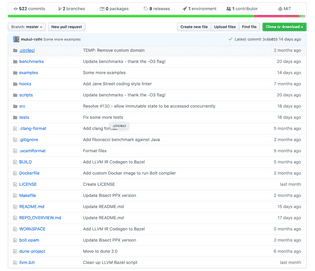
\includegraphics[width=\linewidth]{02_files/repo-overview.png}

%\hypertarget{series-creating-the-bolt-compiler}{%
%\section{Series: Creating the Bolt
%Compiler}\label{series-creating-the-bolt-compiler}}

%\begin{itemize}
%\item
%  { Part 1:
%  }\href{https://mukulrathi.com/create-your-own-programming-language/intro-to-compiler/}{How
%  I wrote my own "proper" programming language}
%\item
%  \textbf{Part 2: So how do you structure a compiler project?}
%\item
%  { Part 3:
%  }\href{https://mukulrathi.com/create-your-own-programming-language/parsing-ocamllex-menhir/}{Writing
%  a Lexer and Parser using OCamllex and Menhir}
%\item
%  { Part 4:
%  }\href{https://mukulrathi.com/create-your-own-programming-language/intro-to-type-checking/}{An
%  accessible introduction to type theory and implementing a
%  type-checker}
%\item
%  { Part 5:
%  }\href{https://mukulrathi.com/create-your-own-programming-language/data-race-dataflow-analysis/}{A
%  tutorial on liveness and alias dataflow analysis}
%\item
%  { Part 6:
%  }\href{https://mukulrathi.com/create-your-own-programming-language/lower-language-constructs-to-llvm/}{Desugaring
%  - taking our high-level language and simplifying it!}
%\item
%  { Part 7:
%  }\href{https://mukulrathi.com/create-your-own-programming-language/protobuf-ocaml-cpp-tutorial/}{A
%  Protobuf tutorial for OCaml and C++}
%\item
%  { Part 8:
%  }\href{https://mukulrathi.com/create-your-own-programming-language/llvm-ir-cpp-api-tutorial/}{A
%  Complete Guide to LLVM for Programming Language Creators}
%\item
%  { Part 9:
%  }\href{https://mukulrathi.com/create-your-own-programming-language/concurrency-runtime-language-tutorial/}{Implementing
%  Concurrency and our Runtime Library}
%\item
%  { Part 10:
%  }\href{https://mukulrathi.com/create-your-own-programming-language/generics-parametric-polymorphism/}{Generics
%  - adding polymorphism to Bolt}
%\item
%  { Part 11:
%  }\href{https://mukulrathi.com/create-your-own-programming-language/inheritance-method-overriding-vtable/}{Adding
%  Inheritance and Method Overriding to Our Language}
%\end{itemize}

\begin{center}\rule{0.5\linewidth}{0.5pt}\end{center}

Writing a compiler is like any other software engineering project in
that it involves a lot of key design decisions: what language do you
use, how do you organise your files in the repo, which tools should you
be using? Most compiler tutorials focus on a toy example and choose to
ignore these practical concerns.

With \emph{Bolt}, I'd like to highlight a larger compiler and the design
decisions I've made. If you're reading this and you work on an
industrial compiler for a more mature language,
\href{https://twitter.com/mukulrathi_}{please reach out on Twitter}! I'd
love to hear about the design decisions you took!

\hypertarget{use-the-right-language-for-the-job-not-just-the-language-you-know-best}{%
\section{\texorpdfstring{\protect\hyperlink{use-the-right-language-for-the-job-not-just-the-language-you-know-best}{}Use
the right language for the job, not just the language you know
best}{Use the right language for the job, not just the language you know best}}\label{use-the-right-language-for-the-job-not-just-the-language-you-know-best}}

\textbf{``Write a compiler using language Y''} (insert your favourite
language) tutorials are a dime a dozen. It might seem easier initially
to write a compiler using a language you know, as it's one less thing to
learn, but this is only a short-term gain. Choosing the correct language
is like learning to touch-type: sure it will be slower to start with,
but just think of how much faster you'll be once you've got to grips
with it!

JavaScript is a great language for web apps and easy to pick up for
beginners. But would I write a compiler in it? \textbf{Frankly, no.} I'm
not hating on JavaScript (I use it in this very site), it just doesn't
suit our goal.

What do we care about for compilers?

\begin{itemize}
\item
  \textbf{Coverage} - we need to consider all possible Bolt expressions
  and make sure we handle all cases - it's no good if our compiler
  crashes on Bolt programs we forgot to consider. Does our language help
  us keep track of this?
\item
  \textbf{Data representation} - how do we represent and manipulate Bolt
  expressions in the compiler?
\item
  \textbf{Tooling} - does our language have libraries we can use for our
  compiler? There's a balance between learning by doing and
  unnecessarily reinventing the wheel.
\item
  \textbf{Speed} - there are two different aspects. Firstly, how fast is
  the compiled Bolt code? Secondly, how fast is the compiler (how long
  does it take to compile the Bolt code)? There's a tradeoff - to get
  faster compiled code, you need to include more optimisation steps in
  your compiler, making the compiler slower.
\end{itemize}

There's no silver bullet: each compiler design inherently has its
tradeoffs. I chose to primarily write my compiler in OCaml.

\hypertarget{why-ocaml}{%
\section{\texorpdfstring{\protect\hyperlink{why-ocaml}{}Why
OCaml?}{Why OCaml?}}\label{why-ocaml}}

OCaml is a functional programming language with a powerful type system.
You probably have two questions: why functional programming, and what do
I mean by powerful type system?

In a large compiler, there's a lot of moving parts and keeping track of
state makes our lives harder. Functional programming is easier to reason
about: if you pass a function the same input it will always return the
same output. With functional programming we don't have to worry about
\textbf{side-effects} or state, and it lets us focus on the high-level
design.

Another alternative is to write the compiler in Rust for performance
reasons. Whilst you might have a faster compiler, I don't think the
speed justifies the additional low-level details like managing memory
that Rust requires you to track. Personally, since I'm not writing
thousands of lines of Bolt code, I'm not too concerned with how long the
Bolt compiler takes to compile programs.

\hypertarget{types-let-you-pair-program-with-the-compiler}{%
\subsection{\texorpdfstring{\protect\hyperlink{types-let-you-pair-program-with-the-compiler}{}Types
let you pair program with the
compiler}{Types let you pair program with the compiler}}\label{types-let-you-pair-program-with-the-compiler}}

If you're coming from a dynamically typed language like JS or Python,
OCaml's rich types can feel alien and may feel cumbersome. The way I
think about types in OCaml is that they give the OCaml compiler more
information about your program - the more you tell it, the more it can
help you!

Coming back to our program of coverage, what we want to say is that a
Bolt expression is \emph{either} an integer, an if-else expression, a
method call, a while loop etc. Normally to represent something like
this, you would use an \texttt{enum} and a \texttt{switch} statement. In
OCaml we bake this ``enum'' into our type system using \emph{variant
types}. We can encode the structure of each expression within the type!
For example, to access a variable you only need to know its name
\texttt{x}. To access an object's field you need to know both its name
\texttt{x} and the field you're accessing \texttt{f}. We can then
\emph{pattern-match} based on each case: think of this like a
\texttt{switch} statement on steroids!

Copy

\begin{lstlisting}[language=caml]
type identifier =| Variable of Var_name.t| ObjField of Var_name.t * Field_name.t
let do_something id = match id with| Var(x) -> ...| ObjField(x,f) -> ...
\end{lstlisting}

I haven't even mentioned the \textbf{best part}. Because we've encoded
our Bolt expression structures in a type, the OCaml compiler will check
if we've covered all cases! That's one less thing for us to track!

So OCaml takes care of coverage, and we've decided that we'll encode
Bolt expressions as variant types, so that's the data representation
sorted. OCaml also has great tooling for the lexer and parser stages of
the compiler (discussed in the next post) which ticks off another of our
criteria.

\hypertarget{targeting-performance-with-llvm}{%
\section{\texorpdfstring{\protect\hyperlink{targeting-performance-with-llvm}{}Targeting
Performance with
LLVM}{Targeting Performance with LLVM}}\label{targeting-performance-with-llvm}}

We touched upon the fact that we don't really care about the performance
of the compiler itself. However, we do want our compiled Bolt code to be
fast (\emph{it's in the name!}). As touched on in the previous post, we
don't have to reinvent the wheel. By targeting \emph{LLVM IR}, we can
hook into the C/C++ toolchain and then get our optimisations for free!

LLVM provide APIs for language authors to generate LLVM IR - the
\emph{native} API is in C++. LLVM also offers bindings in other
languages - they are identical, just replace the C++ syntax with
whichever language you're using. LLVM actually offers OCaml bindings.

\hypertarget{why-is-the-compiler-backend-written-in-c}{%
\subsection{\texorpdfstring{\protect\hyperlink{why-is-the-compiler-backend-written-in-c}{}Why
is the compiler backend written in
C++?}{Why is the compiler backend written in C++?}}\label{why-is-the-compiler-backend-written-in-c}}

A natural question you might ask is: well why didn't you write
everything in OCaml and use the LLVM OCaml bindings?

LLVM's OCaml bindings only map some of the C++ API. At the time of
implementation there was no support for implementing memory fences (a
machine instruction needed to implement locks correctly) so I was forced
to write this part of the compiler in C++. I was also experimenting with
some other fancier memory consistency instructions only present in the
native C++ API.

I want to be frank with you, the OCaml LLVM bindings will likely be
sufficient for your language and I \textbf{encourage you to use that
instead}. See, the tradeoff with the approach I took is that now we have
to pass data between the OCaml compiler \emph{frontend} and the C++
compiler \emph{backend} using
\href{https://mukulrathi.com/create-your-own-programming-language/protobuf-ocaml-cpp-tutorial/}{Protobuf}.
Yes the C++ API has more power, but it results in a more complex
compiler.

Like I said, the LLVM API is the same in OCaml and C++ (apart from
syntax), so this tutorial still applies, just skip the
\href{https://mukulrathi.com/create-your-own-programming-language/protobuf-ocaml-cpp-tutorial/}{Protobuf}
post and use the \href{https://opam.ocaml.org/packages/llvm/}{llvm OCaml
package}!

%\hypertarget{i-make-content-about-my-software-engineering-journey-curated-in-my-newsletter}{%
%\subsection{I make content about my software engineering journey,
%curated in my
%newsletter!}\label{i-make-content-about-my-software-engineering-journey-curated-in-my-newsletter}}
%
%Tips from my time at Cambridge and Facebook, and early access to
%technical tutorials on machine learning, compilers and beyond.
%
%\href{https://newsletter.mukulrathi.com/}{Check out previous issues!}
%
%Email Address
%
%By subscribing, you agree with Revue's
%\href{https://www.getrevue.co/terms}{Terms of Service} and
%\href{https://www.getrevue.co/privacy}{Privacy Policy}.

\hypertarget{software-engineering-methodology}{%
\section{\texorpdfstring{\protect\hyperlink{software-engineering-methodology}{}Software
Engineering
Methodology}{Software Engineering Methodology}}\label{software-engineering-methodology}}

The repository contains more information about how the compiler is
structured in
\href{https://github.com/mukul-rathi/bolt/blob/master/REPO_OVERVIEW.md}{REPO\_OVERVIEW.md}.
Most of these are general software engineering tips so I'll keep this
brief. (If you want more detail, feel free to reach out!)

Firstly, the repository is structured to be \emph{modular}. Each stage
of the compiler has its own library,
\href{http://mukul-rathi.github.io/bolt}{whose documentation you can
view}. Functions are grouped into \emph{modules} (the \texttt{.ml} file
provides the implementation for the module, and the \texttt{.mli} file
provides the module interface). You can think of each module as
performing a certain role within a stage e.g. \texttt{type\_expr.ml}
type-checks expressions, \texttt{pprint\_parser\_tokens.ml}
pretty-prints parser tokens. It makes each module more focused, and
avoids monolithic hundreds-of-lines-long files that are hard to read.

To build these files I use the Dune build system for OCaml (I have a
\href{https://mukulrathi.com/ocaml-tooling-dune/}{blog post explaining
it}) and the Bazel build system for C++. For large repositories,
manually compiling each file (e.g. by running \texttt{clang++\ foo.cpp})
and linking files that depend on each other is nigh on impossible -
build systems automate this for us (running one \texttt{make\ build}
command will compile all the files in the repository). One of the main
benefits of Bazel is that the dependencies are all self-contained so
will work across machines.

For testing, the main library I use is the Jane Street's \textbf{Expect
tests} library. This library is \emph{really easy} to write tests for as
it autogenerates the expected output. I have a
\href{https://mukulrathi.com/ocaml-testing-frameworks/}{blog post on
testing in OCaml} that covers this. The post also explains how I set up
Continuous Integration (where the tests are run and documentation is
generated on each commit to the repository).

I also automate common tasks using a \texttt{Makefile} and
\href{https://github.com/mukul-rathi/bolt/tree/master/scripts}{some
scripts}. One tool I would highly recommend is an autoformatter - I use
\texttt{ocamlformat} for the OCaml code and \texttt{clang-format} for
the C++ code - this formats your code for you so you have pretty looking
code for free! You can automate it with the git pre-commit hook in the
repo (which will lint and format your code every time you're about to
commit) or via IDE format-on-save integration. One final tip: use
\href{https://marketplace.visualstudio.com/items?itemName=freebroccolo.reasonml}{VSCode's
OCaml IDE extension} or the equivalent for your IDE - whenever you hover
over a function it will display its type signature and any documentation
comments associated with it.

\hypertarget{summary}{%
\section{\texorpdfstring{\protect\hyperlink{summary}{}Summary}{Summary}}\label{summary}}

In these first couple of posts, I've explained where Bolt sits in the
spectrum of programming languages, and the compiler design and software
engineering decisions made. In the next post, we'll actually get to
building this. Before we do, I have a couple of action items for you:

\begin{itemize}
\tightlist
\item
  Get up to speed with OCaml.
  \href{https://dev.realworldocaml.org/}{Real World OCaml} is a great
  free resource.
\item
  \href{https://github.com/mukul-rathi/bolt}{Fork the repo.} Have a
  quick high-level scan but don't worry about the details just yet!
  We'll break down each stage of the compiler in its own post, and
  dedicate entire posts to the more complex language features.
\end{itemize}
%
%\hypertarget{share-this-on-twitter}{%
%\subsection{Share This On Twitter}\label{share-this-on-twitter}}
%
%If you liked this post, please consider sharing it with your network. If
%you have any questions, tweet away and I'll answer :) I also tweet when
%new posts drop!
%
%\textbf{PS:} I also share helpful tips and links as I'm learning - so
%you get them \textbf{well before} they make their way into a post!
%
%\hypertarget{series-creating-the-bolt-compiler-1}{%
%\section{Series: Creating the Bolt
%Compiler}\label{series-creating-the-bolt-compiler-1}}
%
%\begin{itemize}
%\item
%  { Part 1:
%  }\href{https://mukulrathi.com/create-your-own-programming-language/intro-to-compiler/}{How
%  I wrote my own "proper" programming language}
%\item
%  \textbf{Part 2: So how do you structure a compiler project?}
%\item
%  { Part 3:
%  }\href{https://mukulrathi.com/create-your-own-programming-language/parsing-ocamllex-menhir/}{Writing
%  a Lexer and Parser using OCamllex and Menhir}
%\item
%  { Part 4:
%  }\href{https://mukulrathi.com/create-your-own-programming-language/intro-to-type-checking/}{An
%  accessible introduction to type theory and implementing a
%  type-checker}
%\item
%  { Part 5:
%  }\href{https://mukulrathi.com/create-your-own-programming-language/data-race-dataflow-analysis/}{A
%  tutorial on liveness and alias dataflow analysis}
%\item
%  { Part 6:
%  }\href{https://mukulrathi.com/create-your-own-programming-language/lower-language-constructs-to-llvm/}{Desugaring
%  - taking our high-level language and simplifying it!}
%\item
%  { Part 7:
%  }\href{https://mukulrathi.com/create-your-own-programming-language/protobuf-ocaml-cpp-tutorial/}{A
%  Protobuf tutorial for OCaml and C++}
%\item
%  { Part 8:
%  }\href{https://mukulrathi.com/create-your-own-programming-language/llvm-ir-cpp-api-tutorial/}{A
%  Complete Guide to LLVM for Programming Language Creators}
%\item
%  { Part 9:
%  }\href{https://mukulrathi.com/create-your-own-programming-language/concurrency-runtime-language-tutorial/}{Implementing
%  Concurrency and our Runtime Library}
%\item
%  { Part 10:
%  }\href{https://mukulrathi.com/create-your-own-programming-language/generics-parametric-polymorphism/}{Generics
%  - adding polymorphism to Bolt}
%\item
%  { Part 11:
%  }\href{https://mukulrathi.com/create-your-own-programming-language/inheritance-method-overriding-vtable/}{Adding
%  Inheritance and Method Overriding to Our Language}
%\end{itemize}
%
%\begin{itemize}
%\item ~
%  \hypertarget{how-i-wrote-my-own-proper-programming-language}{%
%  \subsection{\texorpdfstring{\href{https://mukulrathi.com/create-your-own-programming-language/intro-to-compiler/}{←
%  How I wrote my own "proper" programming
%  language}}{← How I wrote my own "proper" programming language}}\label{how-i-wrote-my-own-proper-programming-language}}
%\item ~
%  \hypertarget{writing-a-lexer-and-parser-using-ocamllex-and-menhir}{%
%  \subsection{\texorpdfstring{\href{https://mukulrathi.com/create-your-own-programming-language/parsing-ocamllex-menhir/}{Writing
%  a Lexer and Parser using OCamllex and Menhir
%  →}}{Writing a Lexer and Parser using OCamllex and Menhir →}}\label{writing-a-lexer-and-parser-using-ocamllex-and-menhir}}
%\end{itemize}
%
%\hypertarget{table-of-contents}{%
%\section{Table of Contents}\label{table-of-contents}}
%
%\href{https://mukulrathi.com/create-your-own-programming-language/compiler-engineering-structure/\#top-of-page}{}
%
%\hypertarget{so-how-do-you-structure-a-compiler-project}{%
%\subsection{So how do you structure a compiler
%project?}\label{so-how-do-you-structure-a-compiler-project}}
%
%\begin{itemize}
%\item
%  \href{https://mukulrathi.com/create-your-own-programming-language/compiler-engineering-structure/\#use-the-right-language-for-the-job-not-just-the-language-you-know-best}{}
%
%  \hypertarget{use-the-right-language-for-the-job-not-just-the-language-you-know-best-1}{%
%  \subsection{Use the right language for the job, not just the
%  language you know
%  best}\label{use-the-right-language-for-the-job-not-just-the-language-you-know-best-1}}
%\item
%  \href{https://mukulrathi.com/create-your-own-programming-language/compiler-engineering-structure/\#why-ocaml}{}
%
%  \hypertarget{why-ocaml-1}{%
%  \subsection{Why OCaml?}\label{why-ocaml-1}}
%
%  \begin{itemize}
%  \item
%    \href{https://mukulrathi.com/create-your-own-programming-language/compiler-engineering-structure/\#types-let-you-pair-program-with-the-compiler}{}
%
%    \hypertarget{types-let-you-pair-program-with-the-compiler-1}{%
%    \subsection{Types let you pair program with the
%    compiler}\label{types-let-you-pair-program-with-the-compiler-1}}
%  \end{itemize}
%\item
%  \href{https://mukulrathi.com/create-your-own-programming-language/compiler-engineering-structure/\#targeting-performance-with-llvm}{}
%
%  \hypertarget{targeting-performance-with-llvm-1}{%
%  \subsection{Targeting Performance with
%  LLVM}\label{targeting-performance-with-llvm-1}}
%
%  \begin{itemize}
%  \item
%    \href{https://mukulrathi.com/create-your-own-programming-language/compiler-engineering-structure/\#why-is-the-compiler-backend-written-in-c}{}
%
%    \hypertarget{why-is-the-compiler-backend-written-in-c-1}{%
%    \subsection{Why is the compiler backend written in
%    C++?}\label{why-is-the-compiler-backend-written-in-c-1}}
%  \end{itemize}
%\item
%  \href{https://mukulrathi.com/create-your-own-programming-language/compiler-engineering-structure/\#software-engineering-methodology}{}
%
%  \hypertarget{software-engineering-methodology-1}{%
%  \subsection{Software Engineering
%  Methodology}\label{software-engineering-methodology-1}}
%\item
%  \href{https://mukulrathi.com/create-your-own-programming-language/compiler-engineering-structure/\#summary}{}
%
%  \hypertarget{summary-1}{%
%  \subsection{Summary}\label{summary-1}}
%\end{itemize}
%
%© Mukul Rathi 2023
%
%\hypertarget{gatsby-announcer}{}
%Navigated to So how do you structure a compiler project?

%\include{chapters/chapter2/ch2}

\part{OCaml Semantic Front End}
%\hypertarget{___gatsby}{}
%\hypertarget{gatsby-focus-wrapper}{}
%\href{https://mukulrathi.com/}{}
%
%MUKUL RATHI
%
%\href{https://mukulrathi.com/about-me}{}
%
%About Me
%
%\href{https://mukulrathi.com/blog}{}
%
%Blog
%
%\hypertarget{creating-the-bolt-compiler-part-3}{%
%\subsection{Creating the Bolt Compiler: Part
%3}\label{creating-the-bolt-compiler-part-3}}

\hypertarget{top-of-page}{%
\chapter{Writing a Lexer and Parser using OCamllex and
Menhir}\label{top-of-page}}

June 01, 2020

%\hypertarget{min-read}{%
%\subsection{10 min read}\label{min-read}}
%
%\hypertarget{last-updated-february-05-2022}{%
%\subsection{Last updated: February 05,
%2022}\label{last-updated-february-05-2022}}

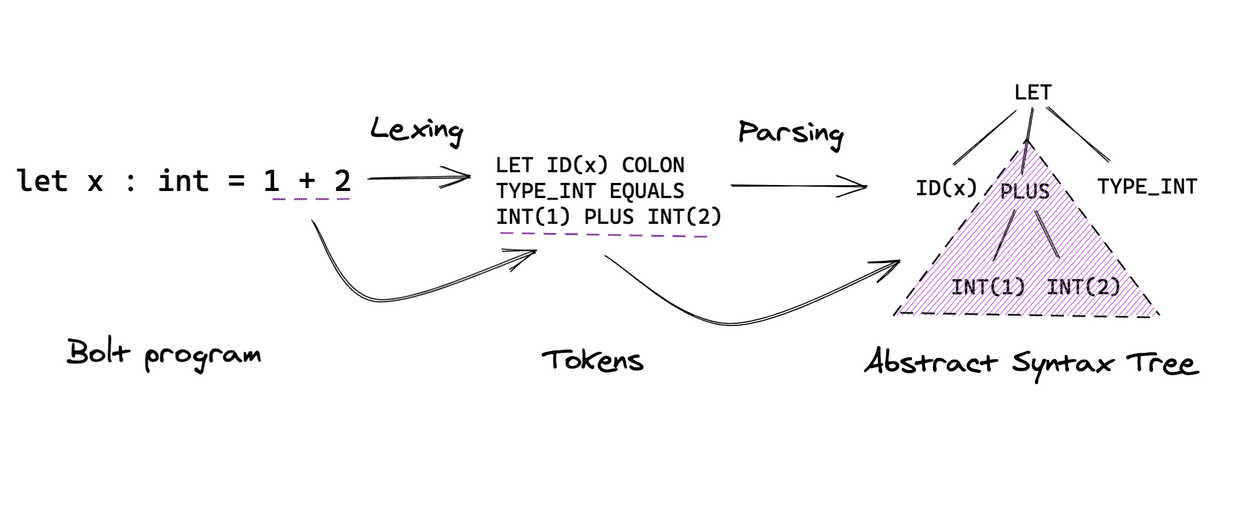
\includegraphics[width=\linewidth]{03_files/parsing-overview.png}

%\hypertarget{series-creating-the-bolt-compiler}{%
%\section{Series: Creating the Bolt
%Compiler}\label{series-creating-the-bolt-compiler}}
%
%\begin{itemize}
%\item
%  { Part 1:
%  }\href{https://mukulrathi.com/create-your-own-programming-language/intro-to-compiler/}{How
%  I wrote my own "proper" programming language}
%\item
%  { Part 2:
%  }\href{https://mukulrathi.com/create-your-own-programming-language/compiler-engineering-structure/}{So
%  how do you structure a compiler project?}
%\item
%  \textbf{Part 3: Writing a Lexer and Parser using OCamllex and Menhir}
%\item
%  { Part 4:
%  }\href{https://mukulrathi.com/create-your-own-programming-language/intro-to-type-checking/}{An
%  accessible introduction to type theory and implementing a
%  type-checker}
%\item
%  { Part 5:
%  }\href{https://mukulrathi.com/create-your-own-programming-language/data-race-dataflow-analysis/}{A
%  tutorial on liveness and alias dataflow analysis}
%\item
%  { Part 6:
%  }\href{https://mukulrathi.com/create-your-own-programming-language/lower-language-constructs-to-llvm/}{Desugaring
%  - taking our high-level language and simplifying it!}
%\item
%  { Part 7:
%  }\href{https://mukulrathi.com/create-your-own-programming-language/protobuf-ocaml-cpp-tutorial/}{A
%  Protobuf tutorial for OCaml and C++}
%\item
%  { Part 8:
%  }\href{https://mukulrathi.com/create-your-own-programming-language/llvm-ir-cpp-api-tutorial/}{A
%  Complete Guide to LLVM for Programming Language Creators}
%\item
%  { Part 9:
%  }\href{https://mukulrathi.com/create-your-own-programming-language/concurrency-runtime-language-tutorial/}{Implementing
%  Concurrency and our Runtime Library}
%\item
%  { Part 10:
%  }\href{https://mukulrathi.com/create-your-own-programming-language/generics-parametric-polymorphism/}{Generics
%  - adding polymorphism to Bolt}
%\item
%  { Part 11:
%  }\href{https://mukulrathi.com/create-your-own-programming-language/inheritance-method-overriding-vtable/}{Adding
%  Inheritance and Method Overriding to Our Language}
%\end{itemize}
%
%\begin{center}\rule{0.5\linewidth}{0.5pt}\end{center}

We can't directly reason about our Bolt program, as it is just an
unstructured stream of characters. Lexing and parsing
\emph{pre-processes} them into a structured representation that we can
perform type-checking on in later stages of the compiler.

\hypertarget{lexing-tokens}{%
\section{\texorpdfstring{\protect\hyperlink{lexing-tokens}{}Lexing
Tokens}{Lexing Tokens}}\label{lexing-tokens}}

The individual characters don't mean much, so first we need to split the
stream into \emph{tokens} (which are analogous to ``words'' in
sentences). These tokens assign meaning: is this group of characters a
specific keyword in our language (\texttt{if} \texttt{int}
\texttt{class}) or is it an identifier (\texttt{banana})?

Tokens also reduce our problem space substantially: they standardise the
representation. We no longer have to worry about whitespace
(\texttt{x\ ==\ 0} and \texttt{x==\ 0} both become
\texttt{IDENTIFIER(x)\ EQUAL\ EQUAL\ INT(0)}) and we can filter out
comments from our source code.

How do we split our stream of characters into tokens? We
\emph{pattern-match}. Under the hood, you could think of this as a
massive case analysis. However, since the case analysis is ambiguous
(multiple tokens could correspond to the same set of characters) we have
two additional rules we have to consider:

\begin{enumerate}
\tightlist
\item
  \textbf{Priority order:} We order our tokens by priority. E.g. we want
  \texttt{int} to be matched as a keyword, not a variable name.
\item
  \textbf{Longest pattern match:} we read \texttt{else} as a keyword
  rather than splitting it into two variable names \texttt{el} and
  \texttt{se}. Likewise, \texttt{intMax} is a variable name: not to be
  read as \texttt{int} and \texttt{Max}.
\end{enumerate}

Here's a really simple lexer that recognises the keywords ``IN'',
``INT'' and identifiers (variable / function names), and tokens are
separating by spaces. Notice we check for the IN case before the
``default'' variable case (priority order):

Copy

\begin{verbatim}
// this is pseudocode for a simplified lexerchars
SeenSoFar = "in"while(streamHasMoreCharacters){  nextChar = readCharFromStream()  if(nextChar == " "){      // we've found a token      switch(charsSeenSoFar):        case "in":          output "IN"          break      case: "int":        output "INT"        break      default:        output ID(charsSeenSoFar)        // not "in" or "int" keywords so must be an identifier      charSeenSoFar= ""  // start matching another token  } else {    // longest match: we'll try to pattern match "int" next iteration    charSeenSoFar += nextChar  }}
\end{verbatim}

\hypertarget{ocamllex}{%
\section{\texorpdfstring{\protect\hyperlink{ocamllex}{}OCamllex}{OCamllex}}\label{ocamllex}}

Whilst you could hand-code the pattern-matching pseudocode, in practice
it is quite finicky especially as our language gets bigger. Instead,
we're going to use the lexer generator \textbf{OCamllex}. OCamllex is an
OCaml library we can use in our compiler by adding it as a dependency to
our Dune build file.

%{
%\href{https://github.com/mukul-rathi/bolt/blob/master/src/frontend/parsing/dune\#L10}{dune}}
%
%Copy

\begin{verbatim}
(ocamllex lexer)
\end{verbatim}

The specification for the lexer is in the \texttt{lexer.mll} file (note
the \texttt{.mll} file extension).

\hypertarget{ocaml-header}{%
\subsection{\texorpdfstring{\protect\hyperlink{ocaml-header}{}OCaml
Header}{OCaml Header}}\label{ocaml-header}}

To start with, we optionally provide a header containing OCaml helper
code (enclosed in curly braces). We define a \texttt{SyntaxError}
exception and a function \texttt{nextline}, which moves the pointer to
the next line of the \texttt{lexbuf} buffer that the program is read
into:

%{
%\href{https://github.com/mukul-rathi/bolt/blob/master/src/frontend/parsing/lexer.mll}{lexer.mll}}
%
%Copy

\begin{lstlisting}[language=caml,caption={{lexer.mll}}]
{open Lexingopen Parser
exception SyntaxError of string
let next_line lexbuf =  let pos = lexbuf.lex_curr_p in  lexbuf.lex_curr_p <-    { pos with pos_bol = lexbuf.lex_curr_pos;               pos_lnum = pos.pos_lnum + 1    }}
\end{lstlisting}

\hypertarget{helper-regexes}{%
\subsection{\texorpdfstring{\protect\hyperlink{helper-regexes}{}Helper
Regexes}{Helper Regexes}}\label{helper-regexes}}

Next, we need to specify the regular expressions we're using to match
the tokens. For most of the tokens, this is a simple string e.g.
\texttt{true} for token \texttt{TRUE}. However, other tokens have more
complex regexes e.g. for integers and identifiers (below).
\href{https://caml.inria.fr/pub/docs/manual-ocaml/lexyacc.html\#ss:ocamllex-regexp}{OCamllex's
regex syntax} is like most regex libraries;
%
%{
%\href{https://github.com/mukul-rathi/bolt/blob/master/src/frontend/parsing/lexer.mll}{lexer.mll}}


\begin{lstlisting}[language=caml,caption={{lexer.mll}}]
(* Define helper regexes *)
let digit = ['0'-'9']let alpha = ['a'-'z' 'A'-'Z']
let int = '-'? digit+  (* regex for integers *)
let id = (alpha) (alpha|digit|'_')* 
(* regex for identifier *)
let whitespace = [' ' '\t']+
let newline = '\r' | '\n' | "\r\n"
\end{lstlisting}

\hypertarget{lexing-rules}{%
\subsection{\texorpdfstring{\protect\hyperlink{lexing-rules}{}Lexing
Rules}{Lexing Rules}}\label{lexing-rules}}

Next, we need to specify rules for OCamllex to scan the input. Each rule
is specified in a pattern-matching format, and we specify the regexes in
order of priority (highest priority first):


\begin{verbatim}
rule <rule_name> = parse | <regex>  {  TOKEN_NAME } (* output a token *)
                   | <regex>  { ... } (* or execute other code *)
and <another_rule> = parse  | ...
\end{verbatim}

The rules are recursive: once it matches a token, it calls itself to
start over and match the next token. Multiple rules are \emph{mutually
recursive}, that is we can recursively call each rule in the other's
definition. Having multiple rules is useful if you want to treat the
character stream differently in different cases.

For example, we want our main rule to read tokens. However, we want to
treat comments differently, not emitting any tokens until we reach the
end of the comment. Another case are strings in Bolt: we want to treat
the characters we are reading as part of a string, not as matching a
token. These cases can all be seen in the following Bolt code:

{example.bolt}

\begin{verbatim}
let x = 4 // here is a comment
/* This is a multi-line   
comment*/
printf("x's value is %d", x)
\end{verbatim}

Now we have our requirements for our lexer, we can define the rules in
our OCamllex specification file. The key points are:

\begin{itemize}
\tightlist
\item
  We have 4 rules: \texttt{read\_token},
  \texttt{read\_single\_line\_comment},
  \texttt{read\_multi\_line\_comment} and \texttt{read\_string}.
\item
  We need to handle \texttt{eof} explicitly (this signifies the end of
  file) and include a catch-all case \texttt{\_} to match all other
  regexes.
\item
  We use \texttt{Lexing.lexeme\ lexbuf} to get the string matched by the
  regex.
\item
  For \texttt{read\_string}, we create another buffer to store the
  characters into: we don't use \texttt{Lexing.lexeme\ lexbuf} as we
  want to explicitly handle escaped characters.
  \texttt{Buffer.create\ 17} allocates a resizable buffer that initially
  has a size of 17 bytes.
\item
  We use \texttt{raise\ SyntaxError} for error-handling (unexpected
  input characters).
\item
  When reading tokens, we skip over whitespace by calling
  \texttt{read\_token\ lexbuf} rather than emitting a token. Likewise,
  for a new line we call our helper function \texttt{next\_line} to skip
  over the new line character.
\end{itemize}

%{
%\href{https://github.com/mukul-rathi/bolt/blob/master/src/frontend/parsing/lexer.mll}{lexer.mll}}


\begin{lstlisting}[caption={{lexer.mll}}]
rule read_token =  parse  
                | "(" { LPAREN }  ... (* keywords and other characters' regexes *)  
                | "printf" {PRINTF }  
                | whitespace { read_token lexbuf }  
                | "//" { single_line_comment lexbuf (* use our comment rule for rest of line *) } 
                | "/*" { multi_line_comment lexbuf }  
                | int { INT (int_of_string (Lexing.lexeme lexbuf))}  
                | id { ID (Lexing.lexeme lexbuf) }    
                | '"'      { read_string (Buffer.create 17) lexbuf }  
                | newline { next_line lexbuf; read_token lexbuf }  
                | eof { EOF }  
                | _ {raise (SyntaxError ("Lexer - Illegal character: " ^ Lexing.lexeme lexbuf)) }
and read_single_line_comment = parse  
                             | newline { next_line lexbuf; read_token lexbuf }  
                             | eof { EOF }  
                             | _ { read_single_line_comment lexbuf }
and read_multi_line_comment = parse  
                            | "*/" { read_token lexbuf }  
                            | newline { next_line lexbuf; read_multi_line_comment lexbuf }  
                            | eof { raise (SyntaxError ("Lexer - Unexpected EOF - please terminate your comment.")) }  
                            | _ { read_multi_line_comment lexbuf }
and read_string buf = parse  
                    | '"'       { STRING (Buffer.contents buf) }  
                    | '\\' 'n'  { Buffer.add_char buf '\n'; read_string buf lexbuf }  
                      ... (* Other regexes to handle escaping special characters *)  
                    | [^ '"' '\\']+    { Buffer.add_string buf (Lexing.lexeme lexbuf);      
                                         read_string buf lexbuf    }  
                    | _ { raise (SyntaxError ("Illegal string character: " ^ Lexing.lexeme lexbuf)) }  
                    | eof { raise (SyntaxError ("String is not terminated")) }
\end{lstlisting}

\hypertarget{generated-ocamllex-output}{%
\subsection{\texorpdfstring{\protect\hyperlink{generated-ocamllex-output}{}Generated
OCamllex
output}{Generated OCamllex output}}\label{generated-ocamllex-output}}

OCamllex generates a \texttt{Lexer} module from the \texttt{lexer.mll}
specification, from which you can call \texttt{Lexer.read\_token} or any
of the other rules, as well as the helper functions defined in the
header. If you're curious, after running \texttt{make\ build} you can
see the generated module in \texttt{lexer.ml} in the \texttt{\_build}
folder - it's just a massive pattern-match statement:




\begin{lstlisting}[language=caml,caption={{\_build/..../lexer.ml}}]
let rec read_token lexbuf =   __ocaml_lex_read_token_rec lexbuf 0and __ocaml_lex_read_token_rec lexbuf __ocaml_lex_state =  match Lexing.engine __ocaml_lex_tables __ocaml_lex_state lexbuf  with| 0 -># 39 "src/frontend/parsing/lexer.mll"        ( LPAREN )# 2603 "src/frontend/parsing/lexer.ml"
  | 1 -># 40 "src/frontend/parsing/lexer.mll"        ( RPAREN )# 2608 "src/frontend/parsing/lexer.ml"
  | 2 -># 41 "src/frontend/parsing/lexer.mll"        ( LBRACE )# 2613 "src/frontend/parsing/lexer.ml"
  | 3 -># 42 "src/frontend/parsing/lexer.mll"        ( RBRACE )# 2618 "src/frontend/parsing/lexer.ml"
  | 4 -># 43 "src/frontend/parsing/lexer.mll"        ( COMMA )# 2623 "src/frontend/parsing/lexer.ml"
\end{lstlisting}

\hypertarget{grammar}{%
\section{\texorpdfstring{\protect\hyperlink{grammar}{}Grammar}{Grammar}}\label{grammar}}

We use structure to reason about sentences - even if we don't think
about it. The words on their own don't tell us much about the sentence -
``use'' is both a noun and verb - it's only because we have a
subject-verb-object pattern in ``we use structure'' can we infer that
``use'' is a verb. The same is true for compilers: The individual tokens
\texttt{x}, \texttt{+}, \texttt{y} don't mean much, but we can infer
from \texttt{x+y} that \texttt{x} and \texttt{y} are numbers being added
together.

We specify the structure of programs in Bolt using a \emph{grammar},
which consists of a set of rules (\emph{productions}) about how we can
construct Bolt expressions.

For example, a program consists of a list of class definitions,
following by some function definitions following by the main expression.
This would look like this (using ``X\_defns'' plural to informally refer
to a list of ``X\_defn'' ).

\textbf{program {{{\(:: =\)}{{{}{::=}}}}} class\_defns function\_defns
main\_expr}

This top level rule also has rules for each of the expressions on the
right hand side. Expressions that can be expanded further with rules are
called \emph{non-terminals}, and those that can't i.e. the tokens are
called \emph{terminals}. Let's look at the \textbf{class\_defn} rule and
\textbf{main\_expr} rules.

A class definition consists of a \texttt{CLASS} keyword token (tokens
are in UPPERCASE) followed by an \texttt{ID} token (identifier = the
class name) and then the body is enclosed by braces. The body consists
of capability definitions (this is Bolt-specific - used to prevent data
races), field definitions and then method definitions. Here the
\texttt{CLASS}, \texttt{ID}, \texttt{LBRACE} and \texttt{RBRACE} tokens
are \emph{terminals}, and the \texttt{capability\_defn},
\texttt{field\_defns} and \texttt{method\_defns} expressions are
\emph{non-terminals} (they have their own rules expanding them).

\textbf{class\_defn {{{\(:: =\)}{{{}{::=}}}}} CLASS ID LBRACE
capability\_defn field\_defns method\_defns RBRACE}

A class definition that satisfies the rules:



%Copy

\begin{lstlisting}[caption={{class\_example.bolt}}]
class Foo { 
    // Foo is the identifier  
    capability linear Bar; // capability definition (has its own rule)  
    // field defns  
    var int f : Bar; 
    // (field has Bolt-specific capability annotatation)  
    const bool g : Bar;  
    //method defns  
    int getF() : Bar {  
       // method definition (again has its own rule)    this.f  
    }
}
\end{lstlisting}

And our main expression has the following rule:

\textbf{main\_expr {{{\(:: =\)}{{{}{::=}}}}} TYPE\_VOID MAIN LPAREN
RPAREN block\_expr}

%{main\_example.bolt}
%
%Copy

\begin{verbatim}
void main() {  ...}
\end{verbatim}

Expressions can have multiple forms:

\textbf{expr {{{\(:: =\)}{{{}{::=}}}}}}

\textbf{\textbar{} NEW ID LPAREN constructor\_args RPAREN}

\textbf{\textbar{} IF expr block\_expr ELSE block\_expr}

\textbf{\textbar{} LET ID EQUAL expr}

and so on.

Full details of Bolt's grammar are in
\href{https://github.com/mukul-rathi/bolt-dissertation/blob/master/dissertation.pdf}{the
appendix of my dissertation}.

\hypertarget{abstract-syntax-trees}{%
\section{\texorpdfstring{\protect\hyperlink{abstract-syntax-trees}{}Abstract
Syntax Trees}{Abstract Syntax Trees}}\label{abstract-syntax-trees}}

If we look at this grammar from another angle, this actually specifies a
hierarchy on our program structure. At the top-level you have our
\textbf{program} rule, and then we recursively expand out each of the
terms on the right-hand-side of the rule (e.g. expand out the class
definition using its rule, main expression using its rule etc.) until we
end up with the tokens.

Which data structure represents hierarchies? \emph{Trees}. So the
grammar also specifies a \emph{syntax tree} for our Bolt program, where
tokens are the leaves.

We could display all tokens on our tree (this would be a \emph{concrete
syntax tree}) but in practice not all tokens are useful. For example, in
the expression \texttt{let\ x\ :\ int\ =\ 1+2}, you care about the
\texttt{ID} token (variable \texttt{x}) and the expression \texttt{1+2}
being assigned to the variable. We don't need to represent the
\texttt{=} token in our tree, as it doesn't convey additional meaning
(we already know we're declaring a variable). By removing these
unnecessary tokens, we end up with an \emph{abstract syntax tree} (AST).

{
\href{https://mukulrathi.com/static/60bd02e28678a6745cea6186af1f8d1b/0da74/concrete-vs-ast.png}{{}
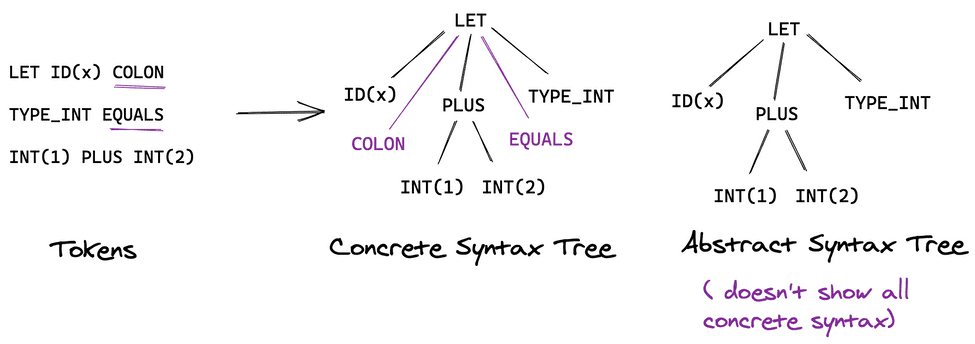
\includegraphics[width=\linewidth]{03_files/concrete-vs-ast.png}} }

The goal of parsing is to construct an Abstract Syntax Tree from a Bolt
program. The subsequent compiler stages then analyse and transform this
parsed AST to form other intermediate ASTs.

Here we split the type definitions for our AST into two files:

\texttt{ast\_types.mli} contains types common to \emph{all} ASTs across
the compiler.
%
%{
%\href{https://github.com/mukul-rathi/bolt/blob/master/src/frontend/ast/ast_types.mli}{ast\_types.mli}}
%
%Copy

\begin{lstlisting}[language=caml,caption={ast\_types.mli}]
(** Stores the line and position of the token *)
type loc = Lexing.position
type bin_op =  | BinOpPlus  | BinOpMinus  | BinOpNotEq
type modifier = MConst  (** Immutable *) 
              | MVar  (** Mutable *)
(** An abstract type for identifiers *)
module type ID = sig  type t
  val of_string : string -> t  
  val to_string : t -> string  
  val ( = ) : t -> t -> boolend
module Var_name : ID
module Class_name : ID
(** Define types of expressions in Bolt programs*)
type type_expr =  | TEInt  | TEClass   of Class_name.t  | TEVoid  | TEBool
  ...
\end{lstlisting}

\texttt{parsed\_ast.mli} contains the OCaml variant types for the class
definitions, function defns and expressions, which are essentially a
mapping of the grammar rules.

%{
%\href{https://github.com/mukul-rathi/bolt/blob/master/src/frontend/parsing/parsed_ast.mli}{parsed\_ast.mli}}
%
%Copy

\begin{lstlisting}[language=caml,caption={{parsed\_ast.mli}}]
type expr =  | Integer     of loc * int  ...  
             | Constructor of loc * Class_name.t * type_expr option * constructor_arg list  (* optional type-parameter *)  
             | Let         of loc * type_expr option * Var_name.t * expr  (* binds variable to expression (optional type annotation) *)  
             | Assign      of loc * identifier * expr  
             | MethodApp   of loc * Var_name.t * Method_name.t * expr list (* read as x.m(args) *)  
             | If          of loc * expr * block_expr * block_expr (* If ___ then ___ else ___ *)  
             | BinOp       of loc * bin_op * expr * expr  ...and block_expr = Block of loc * expr list
type class_defn =  | TClass of Class_name.t * capability list  * field_defn list * method_defn list...
\end{lstlisting}

Note \texttt{Class\_name.t}, \texttt{Var\_name.t} and
\texttt{Method\_name.t} used rather than just a string as these types
give us more information.

\hypertarget{menhir}{%
\section{\texorpdfstring{\protect\hyperlink{menhir}{}Menhir}{Menhir}}\label{menhir}}

As with lexing, we \emph{could} code this up by hand, but it would again
get a lot more finicky as our language scales. We're going to use the
parser generator \textbf{Menhir}. Again as with the lexer, we have a
\texttt{parser.mly} (note \texttt{.mly} extension) specification file.

We need to add Menhir to the Dune build file.

%{
%\href{https://github.com/mukul-rathi/bolt/blob/master/src/frontend/parsing/dune\#L12:L13}{dune}}


\begin{verbatim}
(menhir (modules parser))
\end{verbatim}

Unlike with OCamllex, we also need to update our main Dune project build
file to use Menhir:

%{
%\href{https://github.com/mukul-rathi/bolt/blob/master/dune-project\#L3}{dune-project}}


\begin{lstlisting}[caption={dune-project}]
(using menhir 2.0)
\end{lstlisting}

OCamllex and Menhir have a lot of parallels. We start with our optional
OCaml header (here this just ignores the autogenerated parser file when
calculating test coverage and opens the \texttt{Ast\_types} and
\texttt{Parsed\_ast} modules):

%{
%\href{https://github.com/mukul-rathi/bolt/blob/master/src/frontend/parsing/parser.mly}{parser.mly}}
%

\begin{lstlisting}[caption={parser.mly}]
%{
  [@@@coverage exclude_file]
  open Ast.Ast_types
  open Parsed_ast
%}
\end{lstlisting}

We then specify the tokens we'd defined in OCamllex (OCamllex and Menhir
work seamlessly together):

%{
%\href{https://github.com/mukul-rathi/bolt/blob/master/src/frontend/parsing/parser.mly}{parser.mly}}


\begin{lstlisting}[caption={parser.mly}]
%token  <int> INT
%token  <string> ID
%token  LPAREN
%token  RPAREN...
\end{lstlisting}

\hypertarget{specifying-production-signatures}{%
\subsection{\texorpdfstring{\protect\hyperlink{specifying-production-signatures}{}Specifying
Production
Signatures}{Specifying Production Signatures}}\label{specifying-production-signatures}}

Next, we specify the name of the top-level grammar production (here it
is \texttt{program}):

%{
%\href{https://github.com/mukul-rathi/bolt/blob/master/src/frontend/parsing/parser.mly}{parser.mly}}
%

\begin{lstlisting}[caption={{parser.mly}}]
%start program
\end{lstlisting}

We mentioned earlier that there was a mapping between OCaml variant
types and the grammar productions, now we specify this, so Menhir knows
what type to output when it generates the parser. This is done as a
series of
\texttt{\%type\ \textless{}ast\_type\textgreater{}\ production\_name}:

%{
%\href{https://github.com/mukul-rathi/bolt/blob/master/src/frontend/parsing/parser.mly}{parser.mly}}
%

\begin{lstlisting}[caption={{parser.mly}}]
%type <Parsed_ast.program> program
/* Class defn types */
%type <class_defn> class_defn...
%type <Capability_name.t list> class_capability_annotations
\end{lstlisting}

Note, since we opened the \texttt{Ast\_types} and \texttt{Parsed\_ast}
modules in the header, we can write \texttt{Capability\_name.t} rather
than \texttt{Ast.Ast\_types.Capability\_name.t} and \texttt{class\_defn}
instead of \texttt{Parsed\_ast.class\_defn}. However, we need to specify
absolute types for the top-level production
(\texttt{Parsed\_ast.program} not just \texttt{program}) since this
production is exposed in the \texttt{parser.mli} interface:

\begin{lstlisting}[language=caml,caption={parser.mli}]
(* this file is autogenerated by Menhir *)val program: (Lexing.lexbuf -> token) -> Lexing.lexbuf -> (Parsed_ast.program)
(* if we used program not Parsed_ast.program *)val program: (Lexing.lexbuf -> token) -> Lexing.lexbuf -> (program)(* now parser.mli doesn't know where to find program's type definition *)
\end{lstlisting}

\hypertarget{grammar-rules}{%
\subsection{\texorpdfstring{\protect\hyperlink{grammar-rules}{}Grammar
Rules}{Grammar Rules}}\label{grammar-rules}}

Finally, we can specify our grammar rules, with the returned OCaml
variant expression in \texttt{\{\}} after the rule. We can optionally
separate each of the non-terminal/terminals that make up the
right-hand-side of the rule with semicolons for readability. To use the
result of an expanded non-terminal (e.g. the \texttt{class\_defn}) in
the OCaml expression, we can refer to it with a variable
\texttt{class\_defns} (in general the form is
\texttt{var\_name}=\texttt{nonterminal\ expression}).

%{
%\href{https://github.com/mukul-rathi/bolt/blob/master/src/frontend/parsing/parser.mly}{parser.mly}}
%
%Copy

\begin{lstlisting}[caption={parser.mly}]
program:| class_defns=list(class_defn); function_defns=list(function_defn); main= main_expr;  EOF {Prog(class_defns, function_defns, main)}
\end{lstlisting}

Menhir provides a lot of small helper functions that make writing the
parser easier. We've seen \texttt{list(class\_defn)} - this returns the
type \texttt{Parsed\_ast.class\_defn\ list}. There are other variants of
this e.g. \texttt{separated\_list()} and \texttt{nonempty\_list()} and
\texttt{separated\_nonempty\_list()}:

%{
%\href{https://github.com/mukul-rathi/bolt/blob/master/src/frontend/parsing/parser.mly}{parser.mly}}
%
%Copy

\begin{lstlisting}[caption={parser.mly}]
params:| LPAREN; params=separated_list(COMMA,param); RPAREN {params}
param_capability_annotations:| LBRACE;  capability_names=separated_nonempty_list(COMMA,capability_name); RBRACE {capability_names}
\end{lstlisting}

Another useful function is \texttt{option()}. Here since
\texttt{let\_type\_annot} returns an OCaml expression of type
\texttt{Parsed\_ast.type\_expr}, \texttt{option(let\_type\_annot)}
returns a value of type \texttt{Parsed\_ast.type\_expr\ option} - this
is useful for cases where the user might optionally add type
annotations. e.g. \texttt{let\ x\ :\ int\ =\ 5} vs
\texttt{let\ x\ =\ 5}.

Finally, Menhir also lets us get the line number and position of the
production in the program (we'd defined the type \texttt{loc} for this),
which is useful for error messages! You can decide from where to get the
position: I chose to get the position at the start of the production
using \texttt{\$startpos}.

%{
%\href{https://github.com/mukul-rathi/bolt/blob/master/src/frontend/parsing/parser.mly}{parser.mly}}
%
%Copy

\begin{lstlisting}
expr:| i=INT {Integer($startpos, i)}
     | TRUE { Boolean($startpos, true)}
     | FALSE {  Boolean($startpos, false) }...+
     | e1=expr op=bin_op e2=expr {BinOp($startpos, op, e1, e2)}
     | LET; var_name=ID; type_annot=option(let_type_annot);  EQUAL; bound_expr=expr  {Let($startpos, type_annot, Var_name.of_string var_name, bound_expr)}
     | id=identifier; COLONEQ; assigned_expr=expr {Assign($startpos, id, assigned_expr)}
\end{lstlisting}

\hypertarget{resolving-ambiguous-parses}{%
\subsection{\texorpdfstring{\protect\hyperlink{resolving-ambiguous-parses}{}Resolving
ambiguous
parses}{Resolving ambiguous parses}}\label{resolving-ambiguous-parses}}

Sometimes our grammar can produce \emph{multiple} abstract syntax trees,
in which case we say it is \emph{ambiguous}. The classic example is if
we have the following grammar:

\textbf{expr {{{\(:: =\)}{{{}{::=}}}}} \textbar{} INT \textbar{} expr
PLUS expr \textbar{} expr MULT expr}

{
\href{https://mukulrathi.com/static/23049100e53e9ffd7b0c6afc4e8a1bfd/bf8c1/ambig-parse.png}{{}
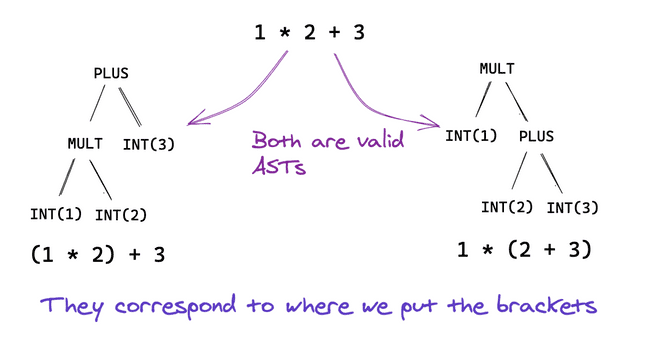
\includegraphics[width=\linewidth]{03_files/ambig-parse.png}} }

If we try to build this grammar with Menhir, then we get the following
error message (the numbers aren't important, Bolt has many more
operators than just + and - ):

%Copy

\begin{verbatim}
menhir src/frontend/parsing/parser.{ml,mli}
Warning: 17 states have shift/reduce conflicts.
Warning: 187 shift/reduce conflicts were arbitrarily resolved.
\end{verbatim}

Arbitrarily resolved isn't good! This means it'll randomly pick one,
even if it's not the one we want. To fix this we have two options

\begin{enumerate}
\tightlist
\item
  Rewrite the grammar to be unambiguous.
\item
  Keep the ambiguity but tell Menhir how to resolve it.
\end{enumerate}

I had initially chosen option 1 for Bolt. It is possible to do this for
\href{https://stackoverflow.com/a/3106287/6752788}{small grammars} but
this becomes harder as your language gets bigger. The main disadvantage
is that you have to put extra parentheses around Bolt expressions to
disambiguate parses, which really isn't a good experience.

When writing this post, I looked at the OCaml compiler for inspiration
(it too uses Menhir!) and the Menhir docs. Option 2 offers a better
solution, but first we need to understand how Menhir works.

Menhir is a \emph{shift-reduce} parser. It builds our AST bottom-up,
deciding based on the next token whether to \emph{reduce} the current
stack of non-terminals and terminals (i.e. it matches the
right-hand-side of a production rule, so reduce it to the
left-hand-side) or to \emph{shift} another token onto the stack.

{
\href{https://mukulrathi.com/static/e2c460bd0a6bcc3f1ab33fc4f962c906/2215f/shift-reduce-parser.png}{{}
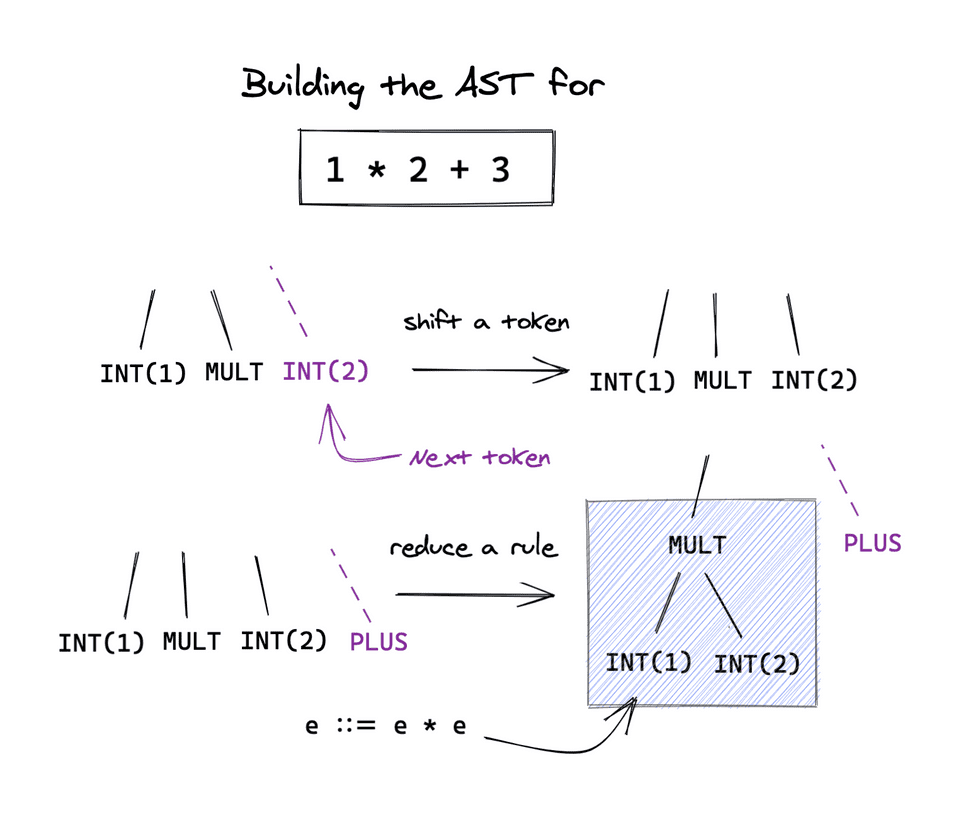
\includegraphics[width=\linewidth]{03_files/shift-reduce-parser.png}} }

A \emph{shift-reduce conflict} occurs when it could do both and end up
with a valid AST in either case. Menhir lets us manually specify which
action to take in the form
\texttt{\textless{}action\textgreater{}\ token} whether the action is:

\begin{enumerate}
\tightlist
\item
  \texttt{\%left}: reduce
\item
  \texttt{\%right}: shift
\item
  \texttt{\%nonassoc}: raise a SyntaxError
\end{enumerate}

If you're not sure which one to choose, you have a secret weapon!

Running \texttt{menhir\ src/frontend/parsing/parser.mly\ -\/-explain}
will generate an explanation in a \texttt{parser.conflicts} file, which
gives an in-depth explanation as to where the conflict is!

This is only part of the story - we want to specify that multiplication
takes precedence over addition. We can do this by specifying an
\emph{ordering} on the actions, from lowest priority to highest. Then
when there are multiple rules, Menhir will choose the one with the
highest priority - it will reduce the multiplication before the addition
in our example, giving us the right AST:

%{
%\href{https://github.com/mukul-rathi/bolt/blob/master/src/frontend/parsing/parser.mly}{parser.mly}}
%
%Copy

\begin{verbatim}
%right  COLONEQ EQUAL
%left PLUS MINUS
%left MULT DIV REM
%nonassoc EXCLAMATION_MARK
\end{verbatim}

So we're done right? Not quite. If we have multiple binary operators,
we'd write this grammar instead as:

\textbf{expr {{{\(:: =\)}{{{}{::=}}}}} \textbar{} INT \textbar{} expr
binop expr}

\textbf{binop {{{\(:: =\)}{{{}{::=}}}}} \textbar{} PLUS \textbar{} MINUS
\textbar{} MULT \textbar{} DIV \textbar{} REM \textbar{} \ldots{}}

After following the steps outlined, you might still get the following
error:

%Copy

\begin{verbatim}
Warning: the precedence level assigned to PLUS is never useful.
\end{verbatim}

Or that you still have shift-reduce conflicts, even though you've
resolved them all. What's gone wrong?

See I said this precedence works if there are \emph{multiple rules}, not
if there is one production. Here we just have the one (\textbf{expr
binop expr}). What we want is one rule for each of the operators
(\textbf{expr PLUS expr}) (\textbf{expr MULT expr}) etc. Menhir's got
you covered - just add an \texttt{\%inline} keyword. This expands all
the uses of \texttt{bin\_op} below to one rule per variant:

%{
%\href{https://github.com/mukul-rathi/bolt/blob/master/src/frontend/parsing/parser.mly}{parser.mly}}
%
%Copy

\begin{verbatim}
%inline bin_op:
| PLUS { BinOpPlus }
| MINUS { BinOpMinus }
| MULT { BinOpMult }...
\end{verbatim}

Et voila, we're done! No more shift-reduce conflicts.

%\hypertarget{i-make-content-about-my-software-engineering-journey-curated-in-my-newsletter}{%
%\subsection{I make content about my software engineering journey,
%curated in my
%newsletter!}\label{i-make-content-about-my-software-engineering-journey-curated-in-my-newsletter}}

%Tips from my time at Cambridge and Facebook, and early access to
%technical tutorials on machine learning, compilers and beyond.

%\href{https://newsletter.mukulrathi.com/}{Check out previous issues!}
%
%Email Address
%
%By subscribing, you agree with Revue's
%\href{https://www.getrevue.co/terms}{Terms of Service} and
%\href{https://www.getrevue.co/privacy}{Privacy Policy}.

\hypertarget{putting-the-lexer-and-parser-together}{%
\section{\texorpdfstring{\protect\hyperlink{putting-the-lexer-and-parser-together}{}Putting
the Lexer and Parser
together}{Putting the Lexer and Parser together}}\label{putting-the-lexer-and-parser-together}}

Right, let's wrap up the \texttt{src/parsing} folder of the Bolt
repository by talking about how we'd put this all together. What we want
is the following:

%{
%\href{https://github.com/mukul-rathi/bolt/blob/master/src/frontend/parsing/lex_and_parse.mli}{lex\_and\_parse.mli}}
%
%Copy

\begin{lstlisting}[caption={lex\_and\_parse.mli},language=caml]
(** Given a lex buffer to read a bolt program from, parse the
    program and return the AST if successful *)
val parse_program : Lexing.lexbuf -> Parsed_ast.program Or_error.t
\end{lstlisting}

To do that, we'll need to use the \texttt{Lexer} and \texttt{Parser}
modules generated by OCamllex and Menhir from our \texttt{lexer.mll} and
\texttt{parser.mly} files. Specifically we care about the two functions:

%Copy

\begin{lstlisting}[language=caml]
val Lexer.read_token: Lexing.lexbuf -> token
val Parser.program: (Lexing.lexbuf -> token) -> Lexing.lexbuf
                    -> (Parsed_ast.program)
\end{lstlisting}

These functions can throw exceptions. It is hard to track which
functions throw exceptions, so we instead catch the exception and
instead use a \texttt{Result} monad (don't be scared!) which has two
possible options - \texttt{Ok\ something} or \texttt{Error\ e}. Then you
can tell from the function signature \texttt{Or\_error.t} that it could
return an error.

%{
%\href{https://github.com/mukul-rathi/bolt/blob/master/src/frontend/parsing/lex_and_parse.ml}{lex\_and\_parse.ml}}
%
%Copy

\begin{lstlisting}[caption={{lex\_and\_parse.ml}},language=caml]
(* Prints the line number and character number where the error occurred.*)
let print_error_position lexbuf =
  let pos = lexbuf.lex_curr_p in
  Fmt.str "Line:%d Position:%d" pos.pos_lnum (pos.pos_cnum - pos.pos_bol + 1)

let parse_program lexbuf =
  try Ok (Parser.program Lexer.read_token lexbuf) with
  (* catch exception and turn into Error *)
  | SyntaxError msg ->
      let error_msg = Fmt.str "%s: %s@." (print_error_position lexbuf) msg in
      Error (Error.of_string error_msg)
  | Parser.Error ->
      let error_msg = Fmt.str "%s: syntax error@." (print_error_position lexbuf) in
      Error (Error.of_string error_msg)

let pprint_parsed_ast ppf (prog : Parsed_ast.program) =
  Pprint_past.pprint_program ppf prog
\end{lstlisting}

This file also exposes the pretty-print function for the parsed AST in
the library (\texttt{pprint\_past.ml}). This is useful for debugging or
expect tests (as this clip of an early version of Bolt demonstrates):

\hypertarget{where-does-this-fit-in-the-bolt-pipeline}{%
\section{\texorpdfstring{\protect\hyperlink{where-does-this-fit-in-the-bolt-pipeline}{}Where
does this fit in the Bolt
pipeline?}{Where does this fit in the Bolt pipeline?}}\label{where-does-this-fit-in-the-bolt-pipeline}}

This is the first stage of the frontend, which can be seen in the
\texttt{compile\_program\_ir} function.

%{
%\href{https://github.com/mukul-rathi/bolt/blob/master/src/frontend/compile_program_ir.ml}{compile\_program\_ir.ml}}
%
%Copy

\begin{lstlisting}[caption={{compile\_program\_ir.ml}},language=caml]
let compile_program_ir ?(should_pprint_past = false) ?(should_pprint_tast = false)
    ?(should_pprint_dast = false) ?(should_pprint_drast = false)
    ?(should_pprint_fir = false) ?(ignore_data_races = false) ?compile_out_file lexbuf =
  let open Result in
  parse_program lexbuf
  >>= maybe_pprint_ast should_pprint_past pprint_parsed_ast
  >>=  ...
\end{lstlisting}

I still haven't told you where the \texttt{lexbuf} comes from. You can
either get it from an input channel, as in the \texttt{main} function,
which reads in a Bolt file from the command line:

%{
%\href{https://github.com/mukul-rathi/bolt/blob/master/src/frontend/main.ml}{main.ml}}
%
%Copy

\begin{lstlisting}[caption={main.ml},language=caml]
In_channel.with_file filename ~f:(fun file_ic ->
            let lexbuf =
              Lexing.from_channel file_ic
              (*Create a lex buffer from the file to read in tokens *) in
            compile_program_ir lexbuf ...
\end{lstlisting}

Or, as in the tests (\texttt{tests/frontend/expect}), you can read from
a string using \texttt{(Lexing.from\_string\ input\_str)}.

\hypertarget{summary}{%
\section{\texorpdfstring{\protect\hyperlink{summary}{}Summary}{Summary}}\label{summary}}

This wraps up the discussion of the lexer and parser. If you haven't
already, \href{https://github.com/mukul-rathi/bolt}{fork the Bolt repo}.

All the code linked in this post is in the \texttt{src/frontend/parsing}
folder, plus some extra rules in the grammar to cover data-race freedom
using \emph{capabilities} (as discussed in
\href{https://github.com/mukul-rathi/bolt-dissertation}{my
dissertation}) and also \emph{inheritance} and \emph{generics}.

Sounds exciting? Next up, we'll talk type-checking and even implement a
form of \emph{local type inference}. The post'll be out within the next
week, and if you enjoyed this post, I'm sure you'll \emph{love} the next
one! I'll explain how to read typing rules
({{{\(\Gamma \vdash e:\tau\)}}})
and how to implement the type checker for the core language.

%\hypertarget{share-this-on-twitter}{%
%\subsection{Share This On Twitter}\label{share-this-on-twitter}}
%
%If you liked this post, please consider sharing it with your network. If
%you have any questions, tweet away and I'll answer :) I also tweet when
%new posts drop!
%
%\textbf{PS:} I also share helpful tips and links as I'm learning - so
%you get them \textbf{well before} they make their way into a post!
%
%\hypertarget{series-creating-the-bolt-compiler-1}{%
%\section{Series: Creating the Bolt
%Compiler}\label{series-creating-the-bolt-compiler-1}}
%
%\begin{itemize}
%\item
%  { Part 1:
%  }\href{https://mukulrathi.com/create-your-own-programming-language/intro-to-compiler/}{How
%  I wrote my own "proper" programming language}
%\item
%  { Part 2:
%  }\href{https://mukulrathi.com/create-your-own-programming-language/compiler-engineering-structure/}{So
%  how do you structure a compiler project?}
%\item
%  \textbf{Part 3: Writing a Lexer and Parser using OCamllex and Menhir}
%\item
%  { Part 4:
%  }\href{https://mukulrathi.com/create-your-own-programming-language/intro-to-type-checking/}{An
%  accessible introduction to type theory and implementing a
%  type-checker}
%\item
%  { Part 5:
%  }\href{https://mukulrathi.com/create-your-own-programming-language/data-race-dataflow-analysis/}{A
%  tutorial on liveness and alias dataflow analysis}
%\item
%  { Part 6:
%  }\href{https://mukulrathi.com/create-your-own-programming-language/lower-language-constructs-to-llvm/}{Desugaring
%  - taking our high-level language and simplifying it!}
%\item
%  { Part 7:
%  }\href{https://mukulrathi.com/create-your-own-programming-language/protobuf-ocaml-cpp-tutorial/}{A
%  Protobuf tutorial for OCaml and C++}
%\item
%  { Part 8:
%  }\href{https://mukulrathi.com/create-your-own-programming-language/llvm-ir-cpp-api-tutorial/}{A
%  Complete Guide to LLVM for Programming Language Creators}
%\item
%  { Part 9:
%  }\href{https://mukulrathi.com/create-your-own-programming-language/concurrency-runtime-language-tutorial/}{Implementing
%  Concurrency and our Runtime Library}
%\item
%  { Part 10:
%  }\href{https://mukulrathi.com/create-your-own-programming-language/generics-parametric-polymorphism/}{Generics
%  - adding polymorphism to Bolt}
%\item
%  { Part 11:
%  }\href{https://mukulrathi.com/create-your-own-programming-language/inheritance-method-overriding-vtable/}{Adding
%  Inheritance and Method Overriding to Our Language}
%\end{itemize}
%
%\begin{itemize}
%\item ~
%  \hypertarget{so-how-do-you-structure-a-compiler-project}{%
%  \subsection{\texorpdfstring{\href{https://mukulrathi.com/create-your-own-programming-language/compiler-engineering-structure/}{←
%  So how do you structure a compiler
%  project?}}{← So how do you structure a compiler project?}}\label{so-how-do-you-structure-a-compiler-project}}
%\item ~
%  \hypertarget{an-accessible-introduction-to-type-theory-and-implementing-a-type-checker}{%
%  \subsection{\texorpdfstring{\href{https://mukulrathi.com/create-your-own-programming-language/intro-to-type-checking/}{An
%  accessible introduction to type theory and implementing a type-checker
%  →}}{An accessible introduction to type theory and implementing a type-checker →}}\label{an-accessible-introduction-to-type-theory-and-implementing-a-type-checker}}
%\end{itemize}
%
%\hypertarget{table-of-contents}{%
%\section{Table of Contents}\label{table-of-contents}}
%
%\href{https://mukulrathi.com/create-your-own-programming-language/parsing-ocamllex-menhir/\#top-of-page}{}
%
%\hypertarget{writing-a-lexer-and-parser-using-ocamllex-and-menhir}{%
%\subsection{Writing a Lexer and Parser using OCamllex and
%Menhir}\label{writing-a-lexer-and-parser-using-ocamllex-and-menhir}}
%
%\begin{itemize}
%\item
%  \href{https://mukulrathi.com/create-your-own-programming-language/parsing-ocamllex-menhir/\#lexing-tokens}{}
%
%  \hypertarget{lexing-tokens-1}{%
%  \subsection{Lexing Tokens}\label{lexing-tokens-1}}
%\item
%  \href{https://mukulrathi.com/create-your-own-programming-language/parsing-ocamllex-menhir/\#ocamllex}{}
%
%  \hypertarget{ocamllex-1}{%
%  \subsection{OCamllex}\label{ocamllex-1}}
%
%  \begin{itemize}
%  \item
%    \href{https://mukulrathi.com/create-your-own-programming-language/parsing-ocamllex-menhir/\#ocaml-header}{}
%
%    \hypertarget{ocaml-header-1}{%
%    \subsection{OCaml Header}\label{ocaml-header-1}}
%  \item
%    \href{https://mukulrathi.com/create-your-own-programming-language/parsing-ocamllex-menhir/\#helper-regexes}{}
%
%    \hypertarget{helper-regexes-1}{%
%    \subsection{Helper Regexes}\label{helper-regexes-1}}
%  \item
%    \href{https://mukulrathi.com/create-your-own-programming-language/parsing-ocamllex-menhir/\#lexing-rules}{}
%
%    \hypertarget{lexing-rules-1}{%
%    \subsection{Lexing Rules}\label{lexing-rules-1}}
%  \item
%    \href{https://mukulrathi.com/create-your-own-programming-language/parsing-ocamllex-menhir/\#generated-ocamllex-output}{}
%
%    \hypertarget{generated-ocamllex-output-1}{%
%    \subsection{Generated OCamllex
%    output}\label{generated-ocamllex-output-1}}
%  \end{itemize}
%\item
%  \href{https://mukulrathi.com/create-your-own-programming-language/parsing-ocamllex-menhir/\#grammar}{}
%
%  \hypertarget{grammar-1}{%
%  \subsection{Grammar}\label{grammar-1}}
%\item
%  \href{https://mukulrathi.com/create-your-own-programming-language/parsing-ocamllex-menhir/\#abstract-syntax-trees}{}
%
%  \hypertarget{abstract-syntax-trees-1}{%
%  \subsection{Abstract Syntax Trees}\label{abstract-syntax-trees-1}}
%\item
%  \href{https://mukulrathi.com/create-your-own-programming-language/parsing-ocamllex-menhir/\#menhir}{}
%
%  \hypertarget{menhir-1}{%
%  \subsection{Menhir}\label{menhir-1}}
%
%  \begin{itemize}
%  \item
%    \href{https://mukulrathi.com/create-your-own-programming-language/parsing-ocamllex-menhir/\#specifying-production-signatures}{}
%
%    \hypertarget{specifying-production-signatures-1}{%
%    \subsection{Specifying Production
%    Signatures}\label{specifying-production-signatures-1}}
%  \item
%    \href{https://mukulrathi.com/create-your-own-programming-language/parsing-ocamllex-menhir/\#grammar-rules}{}
%
%    \hypertarget{grammar-rules-1}{%
%    \subsection{Grammar Rules}\label{grammar-rules-1}}
%  \item
%    \href{https://mukulrathi.com/create-your-own-programming-language/parsing-ocamllex-menhir/\#resolving-ambiguous-parses}{}
%
%    \hypertarget{resolving-ambiguous-parses-1}{%
%    \subsection{Resolving ambiguous
%    parses}\label{resolving-ambiguous-parses-1}}
%  \end{itemize}
%\item
%  \href{https://mukulrathi.com/create-your-own-programming-language/parsing-ocamllex-menhir/\#putting-the-lexer-and-parser-together}{}
%
%  \hypertarget{putting-the-lexer-and-parser-together-1}{%
%  \subsection{Putting the Lexer and Parser
%  together}\label{putting-the-lexer-and-parser-together-1}}
%\item
%  \href{https://mukulrathi.com/create-your-own-programming-language/parsing-ocamllex-menhir/\#where-does-this-fit-in-the-bolt-pipeline}{}
%
%  \hypertarget{where-does-this-fit-in-the-bolt-pipeline-1}{%
%  \subsection{Where does this fit in the Bolt
%  pipeline?}\label{where-does-this-fit-in-the-bolt-pipeline-1}}
%\item
%  \href{https://mukulrathi.com/create-your-own-programming-language/parsing-ocamllex-menhir/\#summary}{}
%
%  \hypertarget{summary-1}{%
%  \subsection{Summary}\label{summary-1}}
%\end{itemize}
%
%© Mukul Rathi 2023
%
%\hypertarget{gatsby-announcer}{}
%Navigated to Writing a Lexer and Parser using OCamllex and Menhir

%\hypertarget{___gatsby}{}
%\hypertarget{gatsby-focus-wrapper}{}
%\href{https://mukulrathi.com/}{}
%
%MUKUL RATHI
%
%\href{https://mukulrathi.com/about-me}{}
%
%About Me
%
%\href{https://mukulrathi.com/blog}{}
%
%Blog
%
%\hypertarget{creating-the-bolt-compiler-part-4}{%
%\subsection{Creating the Bolt Compiler: Part
%4}\label{creating-the-bolt-compiler-part-4}}

\hypertarget{top-of-page}{%
\chapter{An accessible introduction to type theory and implementing a
type-checker}\label{top-of-page}}

June 15, 2020

%\hypertarget{june-15-2020}{%
%\subsection{June 15, 2020}\label{june-15-2020}}
%
%\hypertarget{min-read}{%
%\subsection{11 min read}\label{min-read}}
%
%\hypertarget{last-updated-january-13-2021}{%
%\subsection{Last updated: January 13,
%2021}\label{last-updated-january-13-2021}}
%
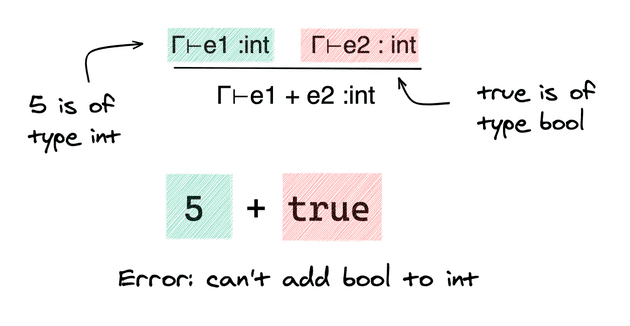
\includegraphics[width=\linewidth]{04_files/type-check.png}
%
%\hypertarget{series-creating-the-bolt-compiler}{%
%\section{Series: Creating the Bolt
%Compiler}\label{series-creating-the-bolt-compiler}}
%
%\begin{itemize}
%\item
%  { Part 1:
%  }\href{https://mukulrathi.com/create-your-own-programming-language/intro-to-compiler/}{How
%  I wrote my own "proper" programming language}
%\item
%  { Part 2:
%  }\href{https://mukulrathi.com/create-your-own-programming-language/compiler-engineering-structure/}{So
%  how do you structure a compiler project?}
%\item
%  { Part 3:
%  }\href{https://mukulrathi.com/create-your-own-programming-language/parsing-ocamllex-menhir/}{Writing
%  a Lexer and Parser using OCamllex and Menhir}
%\item
%  \textbf{Part 4: An accessible introduction to type theory and
%  implementing a type-checker}
%\item
%  { Part 5:
%  }\href{https://mukulrathi.com/create-your-own-programming-language/data-race-dataflow-analysis/}{A
%  tutorial on liveness and alias dataflow analysis}
%\item
%  { Part 6:
%  }\href{https://mukulrathi.com/create-your-own-programming-language/lower-language-constructs-to-llvm/}{Desugaring
%  - taking our high-level language and simplifying it!}
%\item
%  { Part 7:
%  }\href{https://mukulrathi.com/create-your-own-programming-language/protobuf-ocaml-cpp-tutorial/}{A
%  Protobuf tutorial for OCaml and C++}
%\item
%  { Part 8:
%  }\href{https://mukulrathi.com/create-your-own-programming-language/llvm-ir-cpp-api-tutorial/}{A
%  Complete Guide to LLVM for Programming Language Creators}
%\item
%  { Part 9:
%  }\href{https://mukulrathi.com/create-your-own-programming-language/concurrency-runtime-language-tutorial/}{Implementing
%  Concurrency and our Runtime Library}
%\item
%  { Part 10:
%  }\href{https://mukulrathi.com/create-your-own-programming-language/generics-parametric-polymorphism/}{Generics
%  - adding polymorphism to Bolt}
%\item
%  { Part 11:
%  }\href{https://mukulrathi.com/create-your-own-programming-language/inheritance-method-overriding-vtable/}{Adding
%  Inheritance and Method Overriding to Our Language}
%\end{itemize}
%
%\begin{center}\rule{0.5\linewidth}{0.5pt}\end{center}

This post is split into 2 halves: the first half explains the theory
behind type-checkers, and the second half gives you a detailed deep-dive
into how it's implemented in our compiler for our language Bolt. Even if
you aren't interested in writing your own language, the first half is
useful if you've ever heard about \emph{type systems} and want to know
how they even work!

%\hypertarget{share-this-on-twitter}{%
%\subsection{Share This On Twitter}\label{share-this-on-twitter}}
%
%If you find this useful, please share this on Twitter. I'm writing up
%posts on implementing generics and inheritance in this language too!
%
%\includegraphics[width=1.04167in,height=1.11458in]{04_files/profile-pic_004.png}

\hypertarget{what-are-types}{%
\section{\texorpdfstring{\protect\hyperlink{what-are-types}{}What are
types?}{What are types?}}\label{what-are-types}}

We'd discussed this briefly in the first part of the compiler series,
however let's revisit this:

Types are a way of \emph{grouping} program values based on the
\emph{behaviour} we'd like them to have. We have our own ``types'' in
our day-to-day lives. E.g. grouping people as \emph{adults} and
\emph{children}.

Grouping values together means the compiler doesn't have as many cases
to handle. It means we don't need to look at the \emph{actual value}, we
just reason about it based on the \emph{group} it's in (its type).

E.g. the values \texttt{0}, \texttt{1}, \texttt{2}, \texttt{3}\ldots{}
and all other integers are all given the type \texttt{int}. Values of
type \texttt{int} can take part in arithmetic operations like
multiplication on them but we can't concatenate them (like
\texttt{string}s). See how the type (\texttt{int} vs \texttt{string})
defines the \emph{behaviour} of the value (what we can do with them)?

It's even clearer in our custom types. E.g when you define a custom
\texttt{Animal} class with \texttt{eat()} and \texttt{sleep()} methods,
you're saying that objects of type \texttt{Animal} have \texttt{eat} and
\texttt{sleep} behaviour. But we can't divide two \texttt{Animal}
objects by each other - that's not the behaviour we'd allow. What would
\texttt{dog\ /\ cat} even mean?

The role of the \textbf{type-checker} is to prevent this kind of
nonsensical behaviour from happening. That's what we're building today.

All practical languages have type-checking in some form.
\textbf{Statically} typed languages like Rust, Java or Haskell check the
types at \emph{compile-time}. Dynamically-typed languages like JS and
Python \textbf{do} still have types - values are tagged with types at
runtime, and they check types when executing. If you try to run
\texttt{5\ /\ "Hello"}, it won't actually run the code, JS/Python will
see \texttt{"Hello} has type \texttt{string} and will throw a runtime
error instead of executing it.

Right now, this all feels a little hand-wavey. Let's formalise
``preventing nonsensical behaviour''. We want a list of rules to check a
program against, and then if it passes those, we know our program is
safe.

This collection of rules is called a \emph{type system}.

\hypertarget{type-systems}{%
\section{\texorpdfstring{\protect\hyperlink{type-systems}{}Type
Systems}{Type Systems}}\label{type-systems}}

Here's the deal: types define \emph{safe behaviour}. So if we can give
an expression a type, we can use its type to make sure it's being used
in the correct way. The type system's rules (called \emph{typing
judgements}) therefore try to assign a type {{{\(t\)}{{{}{t}}}}} to an
expression {{{\(e\)}{{{}{e}}}}}.

We start by defining seemingly obvious facts, like \texttt{true} is of
type bool. In our type system, the rule is written as follows:

{{\ignoresecond{\(\vdash {\mathbf{t}\mathbf{r}\mathbf{u}\mathbf{e}}:bool\)}{{{}{⊢}{}}{{}{{true}}{}{:}{}}{{}{b}{oo}{l}}}}}

Don't be scared by the maths notation: {{\ignoresecond{\(\vdash\)}{{{}{⊢}}}}} means
``it follows that''. You can read this as ``it follows that the
expression \texttt{true} has type \texttt{bool}. In general,
{{\ignoresecond{\(\vdash \mathbf{e}:t\)}{{{}{⊢}{}}{{}{e}{}{:}{}}{{}{t}}}}} can be
read as ``it follows that expression e has type t''.

Here's a couple more obvious facts.

{{\ignoresecond{\(\vdash {\mathbf{f}\mathbf{a}\mathbf{l}\mathbf{s}\mathbf{e}}:bool\)}{{{}{⊢}{}}{{}{{false}}{}{:}{}}{{}{b}{oo}{l}}}}}

{{\ignoresecond{\(\vdash n:int\)}{{{}{⊢}{}}{{}{n}{}{:}{}}{{}{in}{t}}}}} for any
integer {{{\(n\)}{{{}{n}}}}}.

\hypertarget{typing-environments}{%
\subsection{\texorpdfstring{\protect\hyperlink{typing-environments}{}Typing
environments}{Typing environments}}\label{typing-environments}}

Thing is, looking at an expression on its own isn't always enough for us
to type-check it. What's the type of a variable \texttt{x}? What should
we put in place of the \texttt{?} below?

{{\ignoresecond{\(\vdash x:\ ?\)}{{{}{⊢}{}}{{}{x}{}{:}{~}}{{}{?}}}}}

Well it depends on what type it was given when it was defined. So when
type-checking, we'll need to keep track of the variables' types as they
are defined. We call this the \emph{typing environment}, represented in
our rules as {{\ignoresecond{\(\Gamma\)}{{{}{Γ}}}}} . Think of
{{\ignoresecond{\(\Gamma\)}{{{}{Γ}}}}} as a look-up function that maps variables to
their types.

We update our typing rules to include {{{\(\Gamma\)}}}:

{{{\(\Gamma \vdash \mathbf{x}:t\)}}}.

Back to our typing rule here:

{{{\(\Gamma \vdash x:\ ?\)}}}

\emph{If} {{{\(\Gamma(x) = t\)}},
\emph{then} we can say that:

{{{\(\Gamma \vdash \mathbf{x}:t\)}}}.

In our typing rules we stack these two statements to give one compound
typing rule for variables. This is an example of an \emph{inference}
rule.

{{{\(\frac{\Gamma(x) = t}{\Gamma \vdash x:\ t}\)}}}

\hypertarget{inference-rules}{%
\subsection{\texorpdfstring{\protect\hyperlink{inference-rules}{}Inference
rules}{Inference rules}}\label{inference-rules}}

This odd stacked ``fraction'' is a way of representing deductive
reasoning (like Sherlock Holmes!). If everything on the top holds, then
we \emph{infer} the bottom also holds.

Here's another rule. This says that if we know
{{{\(e_{1}\)}}} and
{{{\(e_{2}\)}}} are
\texttt{int}s, then if we add them together the result is also an
\texttt{int}.

{{\(\frac{\Gamma \vdash e_{1}:int\text{~~~~~~}\Gamma \vdash e_{2}:int}{\Gamma \vdash e_{1} + e_{2}:\ int}\)}}

Using these \emph{inference} rules, we can stack together our pieces of
evidence about different parts of the program to reason about the whole
program. This is how we build up our type system - we \emph{stack} our
rules.

Let's combine what we've learnt so far to type-check a little
expression: \texttt{x\ +\ 1} where our environment
{{{\(\Gamma\)}}} tells us \texttt{x} is an \texttt{int}.

{{{\(\frac{\frac{\frac{}{\Gamma(x) = int}}{\Gamma \vdash x:\ int}\text{~~~~~~}\frac{}{\Gamma \vdash 1:\ int}}{\Gamma \vdash x + 1:\ int}\)}}

Now if it turns out \texttt{x} is an \texttt{string}, then
{{{\(\Gamma(x) = int\)}}} doesn't
hold, so all the rules stacked below it don't hold. Our type-checker
would raise an \emph{error}, as the types don't match up!

\hypertarget{axioms}{%
\subsection{\texorpdfstring{\protect\hyperlink{axioms}{}Axioms}{Axioms}}\label{axioms}}

It's convention here to represent the facts (\emph{axioms}) with a line
above them. You can think them as the ``base case'':

{{{\(\frac{}{\Gamma \vdash 1:\ int}\)}}}

Since they have nothing on the top, technically everything on the top is
true. So the bottom \textbf{always} holds.

If you look back to our example and flip it upside down, it kind of
looks like a tree. It also lays out our reasoning, so acts as a
\emph{proof} - you can just follow the steps. Why is \texttt{x+1} an
int? Well \texttt{x} and \texttt{1} are \texttt{int}s? Why is \texttt{x}
an int? Because\ldots{} You get the idea. So what we've constructed here
is called a \emph{proof tree}.

Okay, let's look at another rule. What about an \texttt{if-else} block?

%Copy

\begin{verbatim}
if (something) {  do_one_thing} else {  do_something_else}
\end{verbatim}

Well, the \texttt{something} has to have type \texttt{bool} as it's a
condition. What about the branches? We need to give this expression an
overall type, but because we're \emph{statically} type-checking, we
don't know which branch will be executed at runtime. Therefore we need
both branches to return the \textbf{same type} (call it
{{{\(t\)}{{{}{t}}}}}), so the expression has the same type
\emph{regardless} of which branch we execute.

{{{\(\frac{\Gamma \vdash e_{1}:bool\text{~~~~~~}\Gamma \vdash e_{2}:t\text{~~~~~~}\Gamma \vdash e_{3}:t}{\Gamma \vdash {\mathbf{i}\mathbf{f}}\ e_{1}\ \{ e_{2}\}\ {\mathbf{e}\mathbf{l}\mathbf{s}\mathbf{e}}\ \{ e_{3}\}:\ t}\)}}}

JavaScript and Python \textbf{would} allow different types for each
branch, since they're doing their type-checking at runtime
(\emph{dynamically} typed), so they know which branch was chosen.

\hypertarget{typing-the-overall-program}{%
\subsection{\texorpdfstring{\protect\hyperlink{typing-the-overall-program}{}Typing
the Overall
Program}{Typing the Overall Program}}\label{typing-the-overall-program}}

This post would end up being too long if I were to list all the rules,
but you can work through each of the cases. We look at the
\emph{grammar} we defined in the previous post and write the
corresponding rules.

We want to show the program is \emph{well-typed} (you can assign it a
type) to show it is safe. So we essentially want a proof tree that shows
it has some type {{{\(t\)}{{{}{t}}}}} (we don't care which):

{{\(\{\}\  \vdash program:\ t\)}}

There's just one thing missing here. Initially
{{{\(\Gamma = \{\}\)}}} - it's empty as we
haven't defined any variables. How do we \textbf{add variables} to
{{\(\Gamma\)}}?

Remember, we add variables to {{{\(\Gamma\)}}} as we declare
them in our program. The syntax for this is a \texttt{let} declaration.
So say we have the following program:

%Copy

\begin{verbatim}
// we have some gamma
let x = e1
// update gamma with x's type
// continue type-checking
e2
\end{verbatim}

We type-check this in the order the program executes:

\begin{itemize}
\tightlist
\item
  We get the type of the expression
  {{\ignoresecond{\(e_{1}\)}{{{}{{e}{{{{{{}{{1}}}}{\hspace{0pt}}}{{{}}}}}}}}}} , call
  it {{{\(t1\)}{{{}{t}{1}}}}}
\item
  We then \emph{extend} the environment {{\ignoresecond{\(\Gamma\)}{{{}{Γ}}}}} with
  the new mapping
  {{\ignoresecond{\(x:t_{1}\)}{{{}{x}{}{:}{}}{{}{{t}{{{{{{}{{1}}}}{\hspace{0pt}}}{{{}}}}}}}}}}.
\item
  We use this extended environment (which we write as
  {{\ignoresecond{\(\Gamma,x:t_{1}\)}{{{}{Γ}{,}{}{x}{}{:}{}}{{}{{t}{{{{{{}{{1}}}}{\hspace{0pt}}}{{{}}}}}}}}}}
  ) to type-check
  {{\ignoresecond{\(e_{2}\)}{{{}{{e}{{{{{{}{{2}}}}{\hspace{0pt}}}{{{}}}}}}}}}} and
  give it type
  {{\ignoresecond{\(t_{2}\)}{{{}{{t}{{{{{{}{{2}}}}{\hspace{0pt}}}{{{}}}}}}}}}}.
\end{itemize}

The whole typing rule thus looks like:

{{\ignoresecond{\(\frac{\Gamma \vdash e_{1}:t_{1}\text{~~~~~}\Gamma,x:t_{1} \vdash e_{2}:t_{2}}{\Gamma \vdash {\mathbf{l}\mathbf{e}\mathbf{t}}\ x = e_{1};\ e_{2}:t_{2}}\)}{{{}{{}{{{{{{}{{Γ}{}{⊢}{}{{let}}{~}{x}{}{=}{}{{e}{{{{{{}{{1}}}}{\hspace{0pt}}}{{{}}}}}}{;}{~}{}{{e}{{{{{{}{{2}}}}{\hspace{0pt}}}{{{}}}}}}{}{:}{}{{t}{{{{{{}{{2}}}}{\hspace{0pt}}}{{{}}}}}}}}{{}{}}{{}{{Γ}{}{⊢}{}{{e}{{{{{{}{{1}}}}{\hspace{0pt}}}{{{}}}}}}{}{:}{}{{t}{{{{{{}{{1}}}}{\hspace{0pt}}}{{{}}}}}}{~}{~}{~}{~}{~}{Γ}{,}{}{x}{}{:}{}{{t}{{{{{{}{{1}}}}{\hspace{0pt}}}{{{}}}}}}{}{⊢}{}{{e}{{{{{{}{{2}}}}{\hspace{0pt}}}{{{}}}}}}{}{:}{}{{t}{{{{{{}{{2}}}}{\hspace{0pt}}}{{{}}}}}}}}}{\hspace{0pt}}}{{{}}}}}{}}}}}}

\hypertarget{type-checking-vs-type-inference}{%
\subsection{\texorpdfstring{\protect\hyperlink{type-checking-vs-type-inference}{}Type
Checking vs Type
Inference}{Type Checking vs Type Inference}}\label{type-checking-vs-type-inference}}

One finer point: here we wrote \texttt{let\ x\ =\ e}. We could have
equally written this as \texttt{let\ x\ :\ t\ =\ e} - where the
programmer \emph{annotates} \texttt{x} with type \texttt{t}. e.g.
\texttt{let\ x\ :\ int\ =\ 1\ +\ 2}.

These lead to different typing algorithms - in the first case the
compiler \emph{infers} that \texttt{1+2} has type \texttt{int}, and in
the second case, the compiler has to \emph{check} that \texttt{1+2} has
type \texttt{int} (since we specified the type \texttt{int} of
\texttt{x}).

As you might imagine, type inference means that the programmer has to
write fewer type annotations, but it is much more complex for the
compiler - it's like filling a Sudoku from scratch versus checking a
Sudoku solution is valid. OCaml and Haskell are examples of languages
with type inference baked in.

In practice, most statically-typed languages do require some type
annotations, but can infer some types (e.g. the \texttt{auto} keyword in
C++). This is like completing a partially solved Sudoku puzzle and is
much easier.

For Bolt, we're going to infer types \emph{within} a function or method
definition, but require programmers to annotate the parameter and return
types. This is a nice middle ground.

%{example\_function.bolt}

%Copy

\begin{verbatim}
function int something(int x, bool y){
  let z = ...
 // z's type is inferred
  ...
}
\end{verbatim}

Okay, enough theory, let's get to implementing this type-checker!

%\hypertarget{i-make-content-about-my-software-engineering-journey-curated-in-my-newsletter}{%
%\subsection{I make content about my software engineering journey,
%curated in my
%newsletter!}\label{i-make-content-about-my-software-engineering-journey-curated-in-my-newsletter}}
%
%Want to learn about how more advanced language features like generics
%and inheritance are typed? Subscribe to receive *exclusive* access to
%future posts before they're released to the general internet.
%
%\href{https://newsletter.mukulrathi.com/}{Check out previous issues!}
%
%Email Address
%
%By subscribing, you agree with Revue's
%\href{https://www.getrevue.co/terms}{Terms of Service} and
%\href{https://www.getrevue.co/privacy}{Privacy Policy}.

\hypertarget{implementing-a-type-checker}{%
\section{\texorpdfstring{\protect\hyperlink{implementing-a-type-checker}{}Implementing
a
Type-checker}{Implementing a Type-checker}}\label{implementing-a-type-checker}}

\hypertarget{just-give-me-the-code}{%
\subsection{\texorpdfstring{\protect\hyperlink{just-give-me-the-code}{}Just
give me the
code!}{Just give me the code!}}\label{just-give-me-the-code}}

You'll need to clone the Bolt repository:

%Copy

\begin{verbatim}
git clone https://github.com/mukul-rathi/bolt
\end{verbatim}

The \href{https://github.com/mukul-rathi/bolt}{Bolt repository}
\texttt{master} branch contains a more complex type-checker, with
support for inheritance, function/method overloading and generics. Each
of these topics will get its own special post later in the series.

So instead, you'll want to look at the \texttt{simple-compiler-tutorial}
release. You can do this as follows:

%Copy

\begin{verbatim}
git checkout simple-compiler-tutorial
\end{verbatim}

This contains a stripped-back version of Bolt from earlier in the
development processs.
\href{https://github.com/mukul-rathi/bolt/tree/simple-compiler-tutorial}{(View
this online)}

The folder we care about is \texttt{src/frontend/typing}.

\hypertarget{a-note-on-ocaml-syntax}{%
\subsection{\texorpdfstring{\protect\hyperlink{a-note-on-ocaml-syntax}{}A
note on OCaml
syntax}{A note on OCaml syntax}}\label{a-note-on-ocaml-syntax}}

In this tutorial we'll be using OCaml syntax. If you're unfamiliar with
this, the main gist is that we'll:

\textbf{a)} Pattern match each of the cases (like \texttt{switch}
statements in other languages). Here we have a variable \texttt{x} and
we do different things based on each of its cases \texttt{A}, \texttt{B}

%Copy

\begin{lstlisting}[language=caml]
match x with  | A -> something  | B -> something_else
\end{lstlisting}

\textbf{b)} Use a Result monad: in essence, this has two values:
\texttt{Ok\ something} and \texttt{Error}. We sequence each of the
operations using the \texttt{\textgreater{}\textgreater{}=} operator -
you don't need to know anything about monads for this tutorial, just
think of this as the same as normal expression sequencing with
\texttt{;}s, just that we're using another operator to represent that
earlier expressions might raise an error.

\hypertarget{types-in-bolt}{%
\subsection{\texorpdfstring{\protect\hyperlink{types-in-bolt}{}Types
in Bolt}{Types in Bolt}}\label{types-in-bolt}}

Bolt has four main types: \texttt{int}, \texttt{bool}, \texttt{void} and
user-defined classes. We represent these four options using a variant
type \texttt{type\_expr} in OCaml:

%{
%\href{https://github.com/mukul-rathi/bolt/blob/simple-compiler-tutorial/src/frontend/ast/ast_types.mli}{ast\_types.mli}}
%
%Copy

\begin{lstlisting}[language=caml,caption={ast\_types.mli}]
type type_expr = TEInt | TEClass of Class_name.t | TEVoid | TEBool
\end{lstlisting}

\hypertarget{annotating-our-ast-with-types}{%
\subsection{\texorpdfstring{\protect\hyperlink{annotating-our-ast-with-types}{}Annotating
our AST with
types}{Annotating our AST with types}}\label{annotating-our-ast-with-types}}

Let's recap our Abstract Syntax Tree from the last part of the series:

%{
%\href{https://github.com/mukul-rathi/bolt/blob/simple-compiler-tutorial/src/frontend/parsing/parsed_ast.mli}{parsed\_ast.mli}}
%
%Copy

\begin{lstlisting}[caption={parsed\_ast.mli},language=caml]
type identifier =
  | Variable of Var_name.t (* x *)
  | ObjField of Var_name.t * Field_name.t (* x.f *)

type expr =
  | Integer     of loc * int (* 1, 2 *)
  | Boolean     of loc * bool (* true*)
  | Identifier  of loc * identifier
  | Constructor of loc * Class_name.t * constructor_arg list (* new Class(args)*)
  | Let         of loc * type_expr option * Var_name.t * expr
    (** let x = e (optional type annotation) *)
  | Assign      of loc * identifier * expr
  | If          of loc * expr * block_expr * block_expr
    (** If ___ then ___ else ___ *)
  ...

and block_expr = Block of loc * expr list
\end{lstlisting}

This AST annotates each expression with \texttt{loc} - the line and
position of the expression. In our type-checking phase, we'll be
checking the types of each of the possible expressions. We'll want to
store our results by \emph{directly annotating} the AST, so the next
compiler stage can view the types just by looking at the AST.

This AST gets the imaginative name \texttt{typed\_ast}:

%{
%\href{https://github.com/mukul-rathi/bolt/blob/simple-compiler-tutorial/src/frontend/typing/typed_ast.mli}{typed\_ast.mli}}
%
%Copy

\begin{lstlisting}[caption={typed\_ast.mli},language=caml]
type identifier =
  | Variable of type_expr * Var_name.t
  | ObjField of Class_name.t * Var_name.t * type_expr * Field_name.t
      (** class of the object, type of field *)

type expr =
  | Integer     of loc * int  (** no need to annotate as obviously TEInt *)
  | Boolean     of loc * bool  (** no need to annotate as obviously TEBool *)
  | Identifier  of loc * identifier  (** Type info associated with identifier *)
  | Constructor of loc * type_expr * Class_name.t * constructor_arg list
  | Let         of loc * type_expr * Var_name.t * expr
  | Assign      of loc * type_expr * identifier * expr
  | If          of loc * type_expr * expr * block_expr * block_expr
      (** the If-else type is that of the branch exprs *)
  ...

and block_expr =
  | Block of loc * type_expr * expr list  (** type is of the final expr in block *)
\end{lstlisting}

We don't annotate obvious types, like for \texttt{Integer} and
\texttt{Boolean}, but we annotate the type of the overall expression for
other expressions e.g. the type returned by an \texttt{if-else}
statement.

A good rule of thumb when annotating the AST is, what would the next
stage need to be told about the program that it can't guess from it
being well-typed? For an \texttt{if-else} statement, if it is well-typed
then the if-condition expression is clearly of type \texttt{bool}, but
we'd need to be told the type of the branches.

\hypertarget{the-type-environment}{%
\subsection{\texorpdfstring{\protect\hyperlink{the-type-environment}{}The
Type Environment}{The Type Environment}}\label{the-type-environment}}

Recall that we used our type environment {{\ignoresecond{\(\Gamma\)}{{{}{Γ}}}}} to
look up the types of variables. We can store this as a list of
\emph{bindings} (variable, type) pairs.

\texttt{type\_env.ml} also contains a ``environment'' of helper
functions that we'll use in this type-checking phase. These are mostly
uninteresting getter methods that you can look at in the repo.

%{
%\href{https://github.com/mukul-rathi/bolt/blob/simple-compiler-tutorial/src/frontend/typing/type_env.mli}{type\_env.mli}}
%
%Copy
\begin{lstlisting}[language=caml,caption={type\_env.mli}]
type type_binding = Var_name.t * type_expr
type type_env = type_binding list

(** A bunch of getter methods used in type-checking the core language *)
val get_var_type : Var_name.t -> type_env -> loc -> type_expr Or_error.t
\end{lstlisting}

It also includes a couple of functions that check we can assign to an
identifier (it's not \texttt{const} or the special identifier
\texttt{this}) and that check we don't have duplicate variable
declarations (shadowing) in the same scope. These again are conceptually
straightforward but are necessary just to cover edge cases.

For example:

\begin{lstlisting}[language=caml,caption={type\_env.ml}]
let check_identifier_assignable class_defns id env loc =
  let open Result in
  match id with
  | Parsed_ast.Variable x ->
      if x = Var_name.of_string "this" then
        Error
          (Error.of_string
             (Fmt.str "%s Type error - Assigning expr to 'this'.@." (string_of_loc loc)))
      else Ok ()
  | Parsed_ast.ObjField (obj_name, field_name) ->
      get_obj_class_defn obj_name env class_defns loc
      >>= fun class_defn ->
      get_class_field field_name class_defn loc
      >>= fun (TField (modifier, _, _, _)) ->
      if modifier = MConst then
        Error
          (Error.of_string
             (Fmt.str "%s Type error - Assigning expr to a const field.@."
                (string_of_loc loc)))
      else Ok ()


\end{lstlisting}

\hypertarget{typing-expressions}{%
\subsection{\texorpdfstring{\protect\hyperlink{typing-expressions}{}Typing
Expressions}{Typing Expressions}}\label{typing-expressions}}

This. This is the \emph{crux} of the implementation. So if you've been
skimming the post, here's where you should pay attention.

What do we need to type-check an expression?

We need the class definitions and function definitions, in case we need
to query the types of fields and function/method type signatures. We
also need the expression itself, and the typing environment we're using
to type-check it.

What do we return? The typed expression, along with its type (we return
type separately to make recursive calls more straightforward). Or we
return an error, if the expression is not well-typed.

Our function type signature captures this exactly:

%{
%\href{https://github.com/mukul-rathi/bolt/blob/simple-compiler-tutorial/src/frontend/typing/type_expr.mli}{type\_expr.mli}}
%
%Copy

\begin{lstlisting}[language=caml,caption={type\_expr.mli}]
val type_expr :
     Parsed_ast.class_defn list
  -> Parsed_ast.function_defn list
  -> Parsed_ast.expr
  -> type_env
  -> (Typed_ast.expr * type_expr) Or_error.t
\end{lstlisting}

In the
\href{https://mukulrathi.com/create-your-own-programming-language/compiler-engineering-structure/}{second
post} in this series, I discussed why we're using OCaml. This stage of
the compiler is one where it really pays off.

For example to type an identifier, we pattern match based on whether it
is a variable \texttt{x} or an object field \texttt{x.f}. If it is a
variable then we get its type from the environment (we pass in
\texttt{loc} as line+position info for error messages). If it returns a
\texttt{var\_type} without an error, then we return the type-annotated
variable.

If it is an object field \texttt{x.f}, then we need to look up the type
of object \texttt{x} in the \texttt{env} and get its corresponding class
definition. We can then look up the type of field \texttt{f} in the
class definition. Then we annotate the identifier with the two bits of
type information we've just learnt: the class of the object, and the
field type.

Our code does exactly that, with no boilerplate:

%{
%\href{https://github.com/mukul-rathi/bolt/blob/simple-compiler-tutorial/src/frontend/typing/type_expr.ml}{type\_expr.ml}}
%
%Copy
\begin{lstlisting}[language=caml,caption={{type\_expr.ml}}]
let type_identifier class_defns identifier env loc =
  let open Result in
  match identifier with
    | Parsed_ast.Variable var_name ->
      get_var_type var_name env loc
      >>| fun var_type -> (Typed_ast.Variable (var_type, var_name), var_type)
  | Parsed_ast.ObjField (var_name, field_name) ->
      get_obj_class_defn var_name env class_defns loc
      >>= fun (Parsed_ast.TClass (class_name, _, _, _) as class_defn) ->
      get_class_field field_name class_defn loc
      >>| fun (TField (_, field_type, _, _)) ->
      (Typed_ast.ObjField (class_name, var_name, field_type, field_name), field_type)
\end{lstlisting}
%\begin{verbatim}
%let type_identifier class_defns identifier env loc =  let open Result in  match identifier with    | Parsed_ast.Variable var_name ->      get_var_type var_name env loc      >>| fun var_type -> (Typed_ast.Variable (var_type, var_name), var_type)  | Parsed_ast.ObjField (var_name, field_name) ->      get_obj_class_defn var_name env class_defns loc      >>= fun (Parsed_ast.TClass (class_name, _, _, _) as class_defn) ->      get_class_field field_name class_defn loc      >>| fun (TField (_, field_type, _, _)) ->      (Typed_ast.ObjField (class_name, var_name, field_type, field_name), field_type)
%\end{verbatim}

Right, so let's look at expressions. This again is clean code that just
reads like our typing judgements. We have \texttt{expr1\ binop\ expr2}
where \texttt{expr1} and \texttt{expr2} are being combined using some
binary operator e.g. \texttt{+}.

Let's remind ourselves of the rule:

{{\ignoresecond{\(\frac{\Gamma \vdash e_{1}:int\text{~~~~~~}\Gamma \vdash e_{2}:int}{\Gamma \vdash e_{1} + e_{2}:\ int}\)}{{{}{{}{{{{{{}{{Γ}{}{⊢}{}{{e}{{{{{{}{{1}}}}{\hspace{0pt}}}{{{}}}}}}{}{+}{}{{e}{{{{{{}{{2}}}}{\hspace{0pt}}}{{{}}}}}}{}{:}{~}{}{in}{t}}}{{}{}}{{}{{Γ}{}{⊢}{}{{e}{{{{{{}{{1}}}}{\hspace{0pt}}}{{{}}}}}}{}{:}{}{in}{t}{~}{~}{~}{~}{~}{~}{Γ}{}{⊢}{}{{e}{{{{{{}{{2}}}}{\hspace{0pt}}}{{{}}}}}}{}{:}{}{in}{t}}}}{\hspace{0pt}}}{{{}}}}}{}}}}}}

What did this say? We type-check the subexpressions
{{\ignoresecond{\(e_{1}\)}{{{}{{e}{{{{{{}{{1}}}}{\hspace{0pt}}}{{{}}}}}}}}}} and
{{\ignoresecond{\(e_{2}\)}{{{}{{e}{{{{{{}{{2}}}}{\hspace{0pt}}}{{{}}}}}}}}}} first.
If they're both \texttt{int}s then the overall expression is an
\texttt{int}.

Here's the main conceptual jump: type-checking each of the expressions
on the top of the judgements corresponds to \emph{recursively} calling
our type-checking function on the subexpressions. We then combine the
results of these type-checking judgments using our rule.

So here, we type-check each of the subexpressions \texttt{expr1} and
\texttt{expr2} (\texttt{type\_with\_defns} just makes the recursive call
shorter).

\begin{lstlisting}[language=caml]
let rec type_expr class_defns function_defns (expr : Parsed_ast.expr) env =
  let open Result in
  let type_with_defns = type_expr class_defns function_defns in
  let type_block_with_defns = type_block_expr class_defns function_defns in match expr with
  | Parsed_ast.BinOp (loc, bin_op, expr1, expr2) -> (
      type_with_defns expr1 env
      >>= fun (typed_expr1, expr1_type) ->
      type_with_defns expr2 env
      >>= fun (typed_expr2, expr2_type) ->
\end{lstlisting}

Recursive calls, check.

Next, because our code deals with more binary operators than just
\texttt{+} we slightly generalise our typing judgement. Regardless of
whether it is \texttt{\&\&} \texttt{+} or \texttt{\textgreater{}}, the
operands \texttt{expr1} and \texttt{expr2} have to have the same type.
Then we check that this type is \texttt{int} for the
\texttt{+\ *\ /\ \%} arithmetic operator cases.

If so, then all \texttt{Ok} and we return \texttt{TEInt} as the type of
the operand.

\begin{lstlisting}[language=caml]
if not (expr1_type = expr2_type) then
        Error ... (* can't have different types *)
      else
        let type_mismatch_error expected_type actual_type = ...
        match bin_op with
        | BinOpPlus | BinOpMinus | BinOpMult | BinOpIntDiv | BinOpRem ->
            if expr1_type = TEInt then
              Ok (Typed_ast.BinOp (loc, TEInt, bin_op, typed_expr1, typed_expr2), TEInt)
            else type_mismatch_error TEInt expr1_type
\end{lstlisting}

As another example of a binary operator, let's look at
\texttt{\textless{}\ \textless{}=\ \textgreater{}\textgreater{}\textgreater{}\ \textgreater{}=}.
These take in integers and return a bool, so we check that the operand
\texttt{expr1} has type \texttt{TEInt} and we return \texttt{TEBool}

%{
%\href{https://github.com/mukul-rathi/bolt/blob/simple-compiler-tutorial/src/frontend/typing/type_expr.ml}{type\_expr.ml}}
%
%Copy

\begin{lstlisting}[language=caml]
| BinOpLessThan | BinOpLessThanEq | BinOpGreaterThan | BinOpGreaterThanEq ->
            if expr1_type = TEInt then
              Ok (Typed_ast.BinOp (loc, TEBool, bin_op, typed_expr1, typed_expr2), TEBool)
            else type_mismatch_error TEInt expr1_type
\end{lstlisting}

Ok, still with me? This post is getting long, so let's just look at
\texttt{if-else} statements and \texttt{let} expressions, and then you
can look at the rest of the code in the repo.

Again, let's remind ourselves of our typing judgement for
\texttt{if-else}.

{{\ignoresecond{\(\frac{\Gamma \vdash e_{1}:bool\text{~~~~~~}\Gamma \vdash e_{2}:t\text{~~~~~~}\Gamma \vdash e_{3}:t}{\Gamma \vdash {\mathbf{i}\mathbf{f}}\ e_{1}\ \{ e_{2}\}\ {\mathbf{e}\mathbf{l}\mathbf{s}\mathbf{e}}\ \{ e_{3}\}:\ t}\)}{{{}{{}{{{{{{}{{Γ}{}{⊢}{}{{if}}{~}{{e}{{{{{{}{{1}}}}{\hspace{0pt}}}{{{}}}}}}{~}{\{}{{e}{{{{{{}{{2}}}}{\hspace{0pt}}}{{{}}}}}}{\}}{~}{{else}}{~}{\{}{{e}{{{{{{}{{3}}}}{\hspace{0pt}}}{{{}}}}}}{\}}{}{:}{~}{}{t}}}{{}{}}{{}{{Γ}{}{⊢}{}{{e}{{{{{{}{{1}}}}{\hspace{0pt}}}{{{}}}}}}{}{:}{}{b}{oo}{l}{~}{~}{~}{~}{~}{~}{Γ}{}{⊢}{}{{e}{{{{{{}{{2}}}}{\hspace{0pt}}}{{{}}}}}}{}{:}{}{t}{~}{~}{~}{~}{~}{~}{Γ}{}{⊢}{}{{e}{{{{{{}{{3}}}}{\hspace{0pt}}}{{{}}}}}}{}{:}{}{t}}}}{\hspace{0pt}}}{{{}}}}}{}}}}}}

That's three expressions on top of the inference rule.

What do these expressions correspond to? Say it with me, \emph{recursive
calls}!

\begin{lstlisting}[language=caml]
| Parsed_ast.If (loc, cond_expr, then_expr, else_expr) -> (
      type_with_defns cond_expr env
      >>= fun (typed_cond_expr, cond_expr_type) ->
      type_block_with_defns then_expr env
      >>= fun (typed_then_expr, then_expr_type) ->
      type_block_with_defns else_expr env
      >>= fun (typed_else_expr, else_expr_type) ->
\end{lstlisting}

Now we need to check that the returned types are what we expected, i.e.
the branches have the same type, and the condition expression has type
\texttt{TEBool}. If that's the case, it's all \texttt{Ok} and we can
return the type of the branch.


\begin{lstlisting}[language=caml]
if not (then_expr_type = else_expr_type) then
        Error ...
      else
        match cond_expr_type with
        | TEBool ->
            Ok
              ( Typed_ast.If
                  (loc, then_expr_type, typed_cond_expr, typed_then_expr, typed_else_expr)
              , then_expr_type )
        | _      ->
            Error ...
\end{lstlisting}

Right, final expression for this post, the \texttt{let} expression,
which looks like this:

{{\ignoresecond{\(\frac{\Gamma \vdash e_{1}:t_{1}\text{~~~~~}\Gamma,x:t_{1} \vdash e_{2}:t_{2}}{\Gamma \vdash {\mathbf{l}\mathbf{e}\mathbf{t}}\ x = e_{1};\ e_{2}:t_{2}}\)}{{{}{{}{{{{{{}{{Γ}{}{⊢}{}{{let}}{~}{x}{}{=}{}{{e}{{{{{{}{{1}}}}{\hspace{0pt}}}{{{}}}}}}{;}{~}{}{{e}{{{{{{}{{2}}}}{\hspace{0pt}}}{{{}}}}}}{}{:}{}{{t}{{{{{{}{{2}}}}{\hspace{0pt}}}{{{}}}}}}}}{{}{}}{{}{{Γ}{}{⊢}{}{{e}{{{{{{}{{1}}}}{\hspace{0pt}}}{{{}}}}}}{}{:}{}{{t}{{{{{{}{{1}}}}{\hspace{0pt}}}{{{}}}}}}{~}{~}{~}{~}{~}{Γ}{,}{}{x}{}{:}{}{{t}{{{{{{}{{1}}}}{\hspace{0pt}}}{{{}}}}}}{}{⊢}{}{{e}{{{{{{}{{2}}}}{\hspace{0pt}}}{{{}}}}}}{}{:}{}{{t}{{{{{{}{{2}}}}{\hspace{0pt}}}{{{}}}}}}}}}{\hspace{0pt}}}{{{}}}}}{}}}}}}

Again, this requires two recursive calls, but note that the second
typing judgement requires the type
{{{\(t_{1}\)}{{{}{{t}{{{{{{}{{1}}}}{\hspace{0pt}}}{{{}}}}}}}}}} of the
first - we need to pass in an extended type environment (after we
type-checked
{{{\(e_{1}\)}{{{}{{e}{{{{{{}{{1}}}}{\hspace{0pt}}}{{{}}}}}}}}}}) to
account for this.

We also have an additional requirement: we want our \texttt{let}
expressions to be \emph{block-scoped}.

%{block\_scoped.bolt}
%
%Copy

\begin{verbatim}
if {
  let x = ...
  // can access x here
} else {
  // shouldn't be able to access x here
}
// or here
\end{verbatim}

So in essence, we want to only update the environment

\begin{enumerate}
\tightlist
\item
  if we have a \texttt{let} expression,
\item
  only for subsequent expressions in the block
\end{enumerate}

We can encode this by \emph{pattern-matching} on our block type-checking
rule. If there are no subsequent expressions (i.e. we have no
expressions (pattern-match on \texttt{{[}{]}}) or just one expression
(pattern-match on \texttt{{[}expr{]}}) in the block), then we don't need
to update our environment.


\begin{lstlisting}[language=caml]
type_block_expr class_defns function_defns (Parsed_ast.Block (loc, exprs)) env =
  ...
  >>= fun () ->
  match exprs with
  | []                      -> Ok (Typed_ast.Block (loc, TEVoid, []), TEVoid) (* empty block has type void *)
  | [expr]                  ->
      type_with_defns expr env
      >>| fun (typed_expr, expr_type) ->
      (Typed_ast.Block (loc, expr_type, [typed_expr]), expr_type)
\end{lstlisting}

Only if we have at least two expressions left in our block
(pattern-match on \texttt{expr1\ ::\ expr2\ ::\ exprs}), and the first
of the two is a \texttt{let} expression do we update the environment for
the rest of the block. We use this updated environment in a recursive
call on \texttt{expr2::exprs} (the remaining expressions). We then
combine the result of the typed blocks.


\begin{lstlisting}
| expr1 :: expr2 :: exprs ->
      type_with_defns expr1 env
      >>= fun (typed_expr1, expr1_type) ->
      (let updated_env =
         match typed_expr1 with
         | Typed_ast.Let (_, _, var_name, _) -> (var_name, expr1_type) :: env
         | _ -> env in
       type_block_with_defns (Parsed_ast.Block (loc, expr2 :: exprs)) updated_env)
      >>| fun (Typed_ast.Block (_, _, typed_exprs), block_expr_type) ->
      (Typed_ast.Block (loc, block_expr_type, typed_expr1 :: typed_exprs), block_expr_type)
\end{lstlisting}

\hypertarget{typing-class-and-function-definitions}{%
\subsection{\texorpdfstring{\protect\hyperlink{typing-class-and-function-definitions}{}Typing
Class and Function
Definitions}{Typing Class and Function Definitions}}\label{typing-class-and-function-definitions}}

We've broken the back of the type-checking now. Let's just wrap up by
checking class and function definitions.

We'll skip over the tedium of checking that there are no duplicate class
definitions or duplicate field definitions in a class etc. (this is in
the repo). Likewise, checking that the types annotated in fields and
method/function type signatures are valids is just a matter of checking
there is a corresponding class definition.

Unlike our main function, for other functions, we don't actually start
with an empty environment when type-checking the function body as we
\emph{already} know the types of some variables - the parameters to the
function!

\begin{lstlisting}[caption={caption text},language=caml]
let init_env_from_params params =
  List.map
    ~f:(function TParam (type_expr, param_name, _, _) -> (param_name, type_expr))
    params
...
type_block_expr class_defns function_defns body_expr(init_env_from_params params)
\end{lstlisting}

%\begin{verbatim}
%let init_env_from_params params =  List.map    ~f:(function TParam (type_expr, param_name, _, _) -> (param_name, type_expr))    params...type_block_expr class_defns function_defns body_expr(init_env_from_params params)
%\end{verbatim}

We also need to check that the type of the result of the body is the
return type (or if it is \texttt{void} then we don't care about the type
returned).

\begin{lstlisting}[language=caml]
>>= fun (typed_body_expr, body_return_type) ->
  (* We throw away returned expr if return type is void *)
  if return_type = TEVoid || body_return_type = return_type then
    Ok
      (Typed_ast.TFunction
         (func_name, maybe_borrowed_ret_ref, return_type, params, typed_body_expr))
  else Error ...
\end{lstlisting}

For class methods, we can initialise the environment and check the
return type in the same way. But we know the type of another special
variable \texttt{this} - the class itself.

\begin{lstlisting}[language=caml,caption={type\_classes.ml}]
let init_env_from_method_params params class_name =
  let param_env =
    List.map
      ~f:(function TParam (type_expr, param_name, _, _) -> (param_name, type_expr))
      params in
  (Var_name.of_string "this", TEClass class_name) :: param_env

\end{lstlisting}

%\begin{verbatim}
%let init_env_from_method_params params class_name =  let param_env =    List.map      ~f:(function TParam (type_expr, param_name, _, _) -> (param_name, type_expr))      params in  (Var_name.of_string "this", TEClass class_name) :: param_env  ```
%\end{verbatim}

\hypertarget{where-does-this-fit-in-the-bolt-pipeline}{%
\section{\texorpdfstring{\protect\hyperlink{where-does-this-fit-in-the-bolt-pipeline}{}Where
does this fit in the Bolt
pipeline?}{Where does this fit in the Bolt pipeline?}}\label{where-does-this-fit-in-the-bolt-pipeline}}

We're two stages into the Bolt compiler pipeline - seen in the
\texttt{compile\_program\_ir} function.
\begin{lstlisting}[caption={{compile\_program\_ir.ml}},language=caml]
let compile_program_ir ?(should_pprint_past = false) ?(should_pprint_tast = false)
    ?(should_pprint_dast = false) ?(should_pprint_drast = false)
    ?(should_pprint_fir = false) ?(ignore_data_races = false) ?compile_out_file lexbuf =
  let open Result in
  parse_program lexbuf
  >>= maybe_pprint_ast should_pprint_past pprint_parsed_ast
  >>= type_program
  >>= maybe_pprint_ast should_pprint_tast pprint_typed_ast
  >>=  ...
\end{lstlisting}

%{
%\href{https://github.com/mukul-rathi/bolt/blob/master/src/frontend/compile_program_ir.ml}{compile\_program\_ir.ml}}
%
%Copy
%
%\begin{verbatim}
%let compile_program_ir ?(should_pprint_past = false) ?(should_pprint_tast = false)    ?(should_pprint_dast = false) ?(should_pprint_drast = false)    ?(should_pprint_fir = false) ?(ignore_data_races = false) ?compile_out_file lexbuf =  let open Result in  parse_program lexbuf  >>= maybe_pprint_ast should_pprint_past pprint_parsed_ast  >>= type_program  >>= maybe_pprint_ast should_pprint_tast pprint_typed_ast  >>=  ...
%\end{verbatim}

\hypertarget{take-away-3-actionable-steps}{%
\section{\texorpdfstring{\protect\hyperlink{take-away-3-actionable-steps}{}Take
Away: 3 Actionable
Steps}{Take Away: 3 Actionable Steps}}\label{take-away-3-actionable-steps}}

If you've got this far, amazing job! The
\href{https://github.com/mukul-rathi/bolt}{Bolt repo} contains the full
code listing with all the typing judgements for each case of the
compiler.

Let's recap what we've done so far:

\begin{enumerate}
\tightlist
\item
  Define what properties in your expression you want to type-check. E.g.
  a condition expression has type \texttt{bool}.
\item
  Formalise this with a typing judgement. Use the \emph{inference} rule
  to reason about subexpressions.
\item
  Map the subexpressions in the inference rule to \emph{recursive}
  calls, then use the inference rule to combine their results.
\end{enumerate}

Next up, we'll talk about the dataflow analysis used to type-check our
linear capabilities in Bolt. This is similar to how the Rust borrow
checker uses ``non-lexical lifetimes'' to check borrowing.

%\hypertarget{share-this-on-twitter-1}{%
%\subsection{Share This On Twitter}\label{share-this-on-twitter-1}}
%
%If you liked this post, please consider sharing it with your network. If
%you have any questions, tweet away and I'll answer :) I also tweet when
%new posts drop!
%
%\textbf{PS:} I also share helpful tips and links as I'm learning - so
%you get them \textbf{well before} they make their way into a post!
%
%\hypertarget{series-creating-the-bolt-compiler-1}{%
%\section{Series: Creating the Bolt
%Compiler}\label{series-creating-the-bolt-compiler-1}}
%
%\begin{itemize}
%\item
%  { Part 1:
%  }\href{https://mukulrathi.com/create-your-own-programming-language/intro-to-compiler/}{How
%  I wrote my own "proper" programming language}
%\item
%  { Part 2:
%  }\href{https://mukulrathi.com/create-your-own-programming-language/compiler-engineering-structure/}{So
%  how do you structure a compiler project?}
%\item
%  { Part 3:
%  }\href{https://mukulrathi.com/create-your-own-programming-language/parsing-ocamllex-menhir/}{Writing
%  a Lexer and Parser using OCamllex and Menhir}
%\item
%  \textbf{Part 4: An accessible introduction to type theory and
%  implementing a type-checker}
%\item
%  { Part 5:
%  }\href{https://mukulrathi.com/create-your-own-programming-language/data-race-dataflow-analysis/}{A
%  tutorial on liveness and alias dataflow analysis}
%\item
%  { Part 6:
%  }\href{https://mukulrathi.com/create-your-own-programming-language/lower-language-constructs-to-llvm/}{Desugaring
%  - taking our high-level language and simplifying it!}
%\item
%  { Part 7:
%  }\href{https://mukulrathi.com/create-your-own-programming-language/protobuf-ocaml-cpp-tutorial/}{A
%  Protobuf tutorial for OCaml and C++}
%\item
%  { Part 8:
%  }\href{https://mukulrathi.com/create-your-own-programming-language/llvm-ir-cpp-api-tutorial/}{A
%  Complete Guide to LLVM for Programming Language Creators}
%\item
%  { Part 9:
%  }\href{https://mukulrathi.com/create-your-own-programming-language/concurrency-runtime-language-tutorial/}{Implementing
%  Concurrency and our Runtime Library}
%\item
%  { Part 10:
%  }\href{https://mukulrathi.com/create-your-own-programming-language/generics-parametric-polymorphism/}{Generics
%  - adding polymorphism to Bolt}
%\item
%  { Part 11:
%  }\href{https://mukulrathi.com/create-your-own-programming-language/inheritance-method-overriding-vtable/}{Adding
%  Inheritance and Method Overriding to Our Language}
%\end{itemize}
%
%\begin{itemize}
%\item ~
%  \hypertarget{writing-a-lexer-and-parser-using-ocamllex-and-menhir}{%
%  \subsection{\texorpdfstring{\href{https://mukulrathi.com/create-your-own-programming-language/parsing-ocamllex-menhir/}{←
%  Writing a Lexer and Parser using OCamllex and
%  Menhir}}{← Writing a Lexer and Parser using OCamllex and Menhir}}\label{writing-a-lexer-and-parser-using-ocamllex-and-menhir}}
%\item ~
%  \hypertarget{a-tutorial-on-liveness-and-alias-dataflow-analysis}{%
%  \subsection{\texorpdfstring{\href{https://mukulrathi.com/create-your-own-programming-language/data-race-dataflow-analysis/}{A
%  tutorial on liveness and alias dataflow analysis
%  →}}{A tutorial on liveness and alias dataflow analysis →}}\label{a-tutorial-on-liveness-and-alias-dataflow-analysis}}
%\end{itemize}
%
%\hypertarget{table-of-contents}{%
%\section{Table of Contents}\label{table-of-contents}}
%
%\href{https://mukulrathi.com/create-your-own-programming-language/intro-to-type-checking/\#top-of-page}{}
%
%\hypertarget{an-accessible-introduction-to-type-theory-and-implementing-a-type-checker}{%
%\subsection{An accessible introduction to type theory and
%implementing a
%type-checker}\label{an-accessible-introduction-to-type-theory-and-implementing-a-type-checker}}
%
%\begin{itemize}
%\item
%  \href{https://mukulrathi.com/create-your-own-programming-language/intro-to-type-checking/\#what-are-types}{}
%
%  \hypertarget{what-are-types-1}{%
%  \subsection{What are types?}\label{what-are-types-1}}
%\item
%  \href{https://mukulrathi.com/create-your-own-programming-language/intro-to-type-checking/\#type-systems}{}
%
%  \hypertarget{type-systems-1}{%
%  \subsection{Type Systems}\label{type-systems-1}}
%
%  \begin{itemize}
%  \item
%    \href{https://mukulrathi.com/create-your-own-programming-language/intro-to-type-checking/\#typing-environments}{}
%
%    \hypertarget{typing-environments-1}{%
%    \subsection{Typing environments}\label{typing-environments-1}}
%  \item
%    \href{https://mukulrathi.com/create-your-own-programming-language/intro-to-type-checking/\#inference-rules}{}
%
%    \hypertarget{inference-rules-1}{%
%    \subsection{Inference rules}\label{inference-rules-1}}
%  \item
%    \href{https://mukulrathi.com/create-your-own-programming-language/intro-to-type-checking/\#axioms}{}
%
%    \hypertarget{axioms-1}{%
%    \subsection{Axioms}\label{axioms-1}}
%  \item
%    \href{https://mukulrathi.com/create-your-own-programming-language/intro-to-type-checking/\#typing-the-overall-program}{}
%
%    \hypertarget{typing-the-overall-program-1}{%
%    \subsection{Typing the Overall
%    Program}\label{typing-the-overall-program-1}}
%  \item
%    \href{https://mukulrathi.com/create-your-own-programming-language/intro-to-type-checking/\#type-checking-vs-type-inference}{}
%
%    \hypertarget{type-checking-vs-type-inference-1}{%
%    \subsection{Type Checking vs Type
%    Inference}\label{type-checking-vs-type-inference-1}}
%  \end{itemize}
%\item
%  \href{https://mukulrathi.com/create-your-own-programming-language/intro-to-type-checking/\#implementing-a-type-checker}{}
%
%  \hypertarget{implementing-a-type-checker-1}{%
%  \subsection{Implementing a
%  Type-checker}\label{implementing-a-type-checker-1}}
%
%  \begin{itemize}
%  \item
%    \href{https://mukulrathi.com/create-your-own-programming-language/intro-to-type-checking/\#just-give-me-the-code}{}
%
%    \hypertarget{just-give-me-the-code-1}{%
%    \subsection{Just give me the
%    code!}\label{just-give-me-the-code-1}}
%  \item
%    \href{https://mukulrathi.com/create-your-own-programming-language/intro-to-type-checking/\#a-note-on-ocaml-syntax}{}
%
%    \hypertarget{a-note-on-ocaml-syntax-1}{%
%    \subsection{A note on OCaml
%    syntax}\label{a-note-on-ocaml-syntax-1}}
%  \item
%    \href{https://mukulrathi.com/create-your-own-programming-language/intro-to-type-checking/\#types-in-bolt}{}
%
%    \hypertarget{types-in-bolt-1}{%
%    \subsection{Types in Bolt}\label{types-in-bolt-1}}
%  \item
%    \href{https://mukulrathi.com/create-your-own-programming-language/intro-to-type-checking/\#annotating-our-ast-with-types}{}
%
%    \hypertarget{annotating-our-ast-with-types-1}{%
%    \subsection{Annotating our AST with
%    types}\label{annotating-our-ast-with-types-1}}
%  \item
%    \href{https://mukulrathi.com/create-your-own-programming-language/intro-to-type-checking/\#the-type-environment}{}
%
%    \hypertarget{the-type-environment-1}{%
%    \subsection{The Type Environment}\label{the-type-environment-1}}
%  \item
%    \href{https://mukulrathi.com/create-your-own-programming-language/intro-to-type-checking/\#typing-expressions}{}
%
%    \hypertarget{typing-expressions-1}{%
%    \subsection{Typing Expressions}\label{typing-expressions-1}}
%  \item
%    \href{https://mukulrathi.com/create-your-own-programming-language/intro-to-type-checking/\#typing-class-and-function-definitions}{}
%
%    \hypertarget{typing-class-and-function-definitions-1}{%
%    \subsection{Typing Class and Function
%    Definitions}\label{typing-class-and-function-definitions-1}}
%  \end{itemize}
%\item
%  \href{https://mukulrathi.com/create-your-own-programming-language/intro-to-type-checking/\#where-does-this-fit-in-the-bolt-pipeline}{}
%
%  \hypertarget{where-does-this-fit-in-the-bolt-pipeline-1}{%
%  \subsection{Where does this fit in the Bolt
%  pipeline?}\label{where-does-this-fit-in-the-bolt-pipeline-1}}
%\item
%  \href{https://mukulrathi.com/create-your-own-programming-language/intro-to-type-checking/\#take-away-3-actionable-steps}{}
%
%  \hypertarget{take-away-3-actionable-steps-1}{%
%  \subsection{Take Away: 3 Actionable
%  Steps}\label{take-away-3-actionable-steps-1}}
%\end{itemize}
%
%© Mukul Rathi 2023
%
%\hypertarget{gatsby-announcer}{}
%Navigated to An accessible introduction to type theory and implementing
%a type-checker

%\hypertarget{___gatsby}{}
%\hypertarget{gatsby-focus-wrapper}{}
%\href{https://mukulrathi.com/}{}
%
%MUKUL RATHI
%
%\href{https://mukulrathi.com/about-me}{}
%
%About Me
%
%\href{https://mukulrathi.com/blog}{}
%
%Blog
%
%\hypertarget{creating-the-bolt-compiler-part-5}{%
%\subsection{Creating the Bolt Compiler: Part
%5}\label{creating-the-bolt-compiler-part-5}}

\hypertarget{top-of-page}{%
\chapter{A tutorial on liveness and alias dataflow
analysis}\label{top-of-page}}

June 27, 2020

%\hypertarget{june-27-2020}{%
%\subsection{June 27, 2020}\label{june-27-2020}}
%
%\hypertarget{min-read}{%
%\subsection{7 min read}\label{min-read}}
%
%\hypertarget{last-updated-december-20-2020}{%
%\subsection{Last updated: December 20,
%2020}\label{last-updated-december-20-2020}}
%
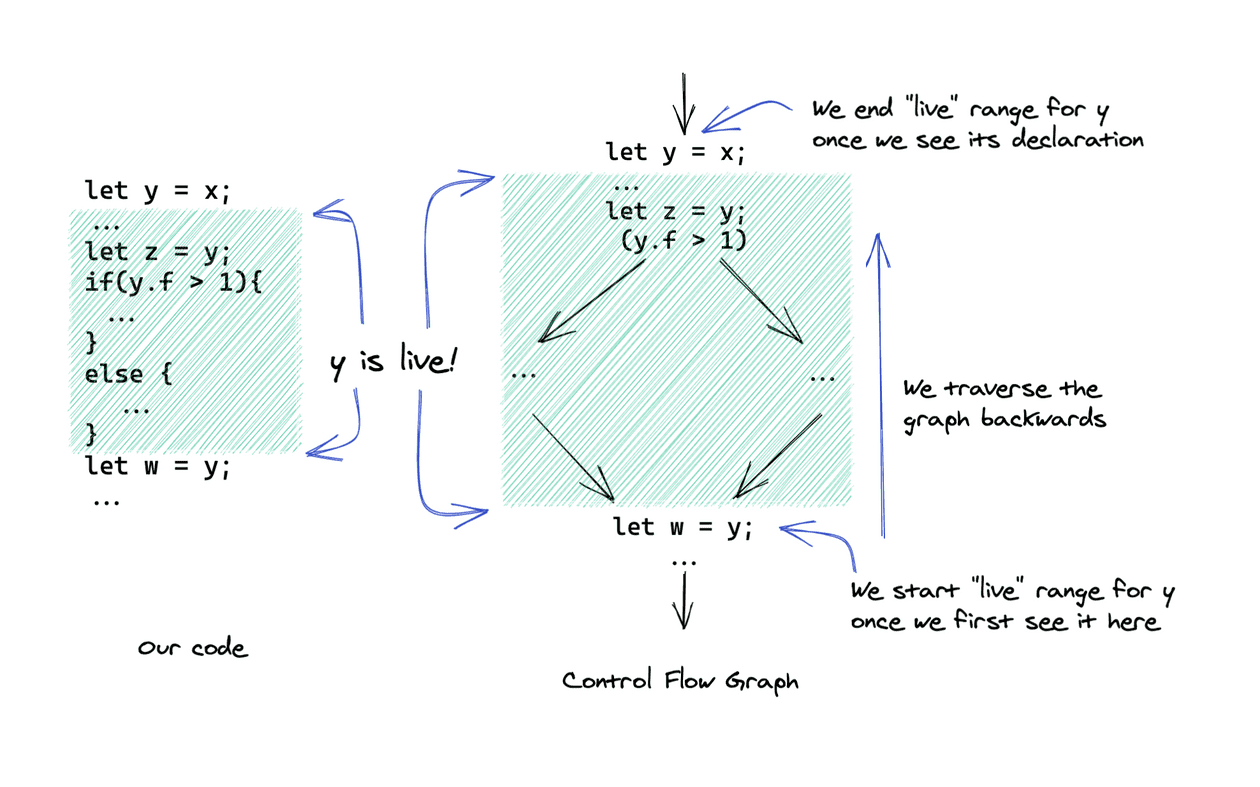
\includegraphics[width=\linewidth]{05_files/liveness-range.png}
%
%\hypertarget{series-creating-the-bolt-compiler}{%
%\section{Series: Creating the Bolt
%Compiler}\label{series-creating-the-bolt-compiler}}
%
%\begin{itemize}
%\item
%  { Part 1:
%  }\href{https://mukulrathi.com/create-your-own-programming-language/intro-to-compiler/}{How
%  I wrote my own "proper" programming language}
%\item
%  { Part 2:
%  }\href{https://mukulrathi.com/create-your-own-programming-language/compiler-engineering-structure/}{So
%  how do you structure a compiler project?}
%\item
%  { Part 3:
%  }\href{https://mukulrathi.com/create-your-own-programming-language/parsing-ocamllex-menhir/}{Writing
%  a Lexer and Parser using OCamllex and Menhir}
%\item
%  { Part 4:
%  }\href{https://mukulrathi.com/create-your-own-programming-language/intro-to-type-checking/}{An
%  accessible introduction to type theory and implementing a
%  type-checker}
%\item
%  \textbf{Part 5: A tutorial on liveness and alias dataflow analysis}
%\item
%  { Part 6:
%  }\href{https://mukulrathi.com/create-your-own-programming-language/lower-language-constructs-to-llvm/}{Desugaring
%  - taking our high-level language and simplifying it!}
%\item
%  { Part 7:
%  }\href{https://mukulrathi.com/create-your-own-programming-language/protobuf-ocaml-cpp-tutorial/}{A
%  Protobuf tutorial for OCaml and C++}
%\item
%  { Part 8:
%  }\href{https://mukulrathi.com/create-your-own-programming-language/llvm-ir-cpp-api-tutorial/}{A
%  Complete Guide to LLVM for Programming Language Creators}
%\item
%  { Part 9:
%  }\href{https://mukulrathi.com/create-your-own-programming-language/concurrency-runtime-language-tutorial/}{Implementing
%  Concurrency and our Runtime Library}
%\item
%  { Part 10:
%  }\href{https://mukulrathi.com/create-your-own-programming-language/generics-parametric-polymorphism/}{Generics
%  - adding polymorphism to Bolt}
%\item
%  { Part 11:
%  }\href{https://mukulrathi.com/create-your-own-programming-language/inheritance-method-overriding-vtable/}{Adding
%  Inheritance and Method Overriding to Our Language}
%\end{itemize}
%
%\begin{center}\rule{0.5\linewidth}{0.5pt}\end{center}

\hypertarget{dataflow-analysis---the-big-picture}{%
\section{\texorpdfstring{\protect\hyperlink{dataflow-analysis---the-big-picture}{}Dataflow
Analysis - the big
picture}{Dataflow Analysis - the big picture}}\label{dataflow-analysis---the-big-picture}}

In the previous post in the series, we looked at how type-checking the
core language worked. This analysis is \emph{flow-insensitive} - it does
not depend on the flow of the execution of the program. If an expression
is of type \texttt{int} then it will have type \texttt{int} regardless
of what was executed before or after it.

Some program properties do however depend on the execution path taken by
a program. Dataflow analysis tracks how a particular value might
propagate as the program executes.

For example, a value might \emph{alias} - you could have multiple
references pointing to that value. Whether two references \texttt{x} and
\texttt{y} alias can't be determined by looking at their assignments in
isolation - we need to track the execution to determine if they have the
same value assigned to them.

%{alias\_example}

%Copy

\begin{verbatim}
let x = someObject...
let y = someObject 
// x and y alias as both point to same object
\end{verbatim}

Another example is \textbf{liveness analysis} - we say a value is
\emph{live} if some point later in the program it could be used, and
\emph{dead} otherwise.

%{liveness\_example}

%Copy

\begin{verbatim}
let x = someValue 
// someValue is live...
print(x) // as we use someValue here
x = someOtherValue 
// someOtherValue isn't used - so dead
\end{verbatim}

Why do we care about alias analysis and liveness analysis? Well it turns
out that Rust's \emph{borrow-checker} uses a combination of these to
determine when a reference is borrowed. Bolt has a \emph{linear}
capability in its type system which acts the same.

Both Rust's borrow checker and Bolt's capabilities prevent data races -
an explanation why is in
\href{https://github.com/mukul-rathi/bolt-dissertation/blob/master/dissertation.pdf}{my
dissertation}.

In a nutshell, Rust works on the principle of \textbf{ownership}: you
either have one reference (owner) that can read/write (a \emph{mutable}
reference) or you can \emph{borrow} (aka alias) the reference.

To enforce this we care about 2 things:

\begin{enumerate}
\tightlist
\item
  When is a reference borrowed? (alias analysis)
\item
  For how long is it borrowed? (liveness analysis)
\end{enumerate}

Let's elaborate on that second point. When is a reference borrowed? The
first version of Rust's borrow checker said this was whilst an alias was
in scope.

{borrow\_example}

Copy

\begin{verbatim}
let x = something 
// this is pseudocode not Rust
{  let y = x  ...
   // y will be used in future
  print(y)
  // no longer using y
  x = somethingElse
}// y is out of scope
\end{verbatim}

That means we cannot reassign \texttt{x} in the example until \texttt{y}
is out of scope. This is a ``lexical lifetime'' - \texttt{y}'s borrow
lifetime is determined by its lexical scope. So that means \texttt{x}
can't be reassigned, since it is borrowed at that point. But \texttt{y}
isn't being used so surely \texttt{x} isn't still borrowed?

That's the idea behind \textbf{non-lexical lifetimes} - the borrow ends
when the value of \texttt{y} is dead - i.e. it is not being used.

In Bolt, we'll be tracking the lifetimes of references to
\emph{objects}.

Let's get implementing it!

\hypertarget{alias-analysis}{%
\section{\texorpdfstring{\protect\hyperlink{alias-analysis}{}Alias
Analysis}{Alias Analysis}}\label{alias-analysis}}

The first step is to determine when two values alias. How do we know two
references will point to the same object without actually executing the
program?

We use \textbf{abstract interpretation}.

\hypertarget{abstract-interpretation}{%
\subsection{\texorpdfstring{\protect\hyperlink{abstract-interpretation}{}Abstract
Interpretation}{Abstract Interpretation}}\label{abstract-interpretation}}

Abstract interpretation is the process of simulating the execution of
the program but only storing the program properties we care about. So in
our case, we don't care about what the actual result of the program
execution is, we're just tracking the \emph{set of aliases}.

Implicit in this is a set of rules for how the program will execute, we
call this its \textbf{operational semantics}. We will not go into
details here, but it's things like:

\begin{itemize}
\tightlist
\item
  Do we evaluate expressions left-to-right or right-to-left?
\item
  When calling a function, do we fully evaluate the argument expression
  and then call the function with the value of that argument, or do we
  just plug in the unevaluated argument expression directly into the
  function and only evaluate it at the point it is used in the function
  body? The former is called \textbf{call-by-value} and is used in most
  mainstream languages like Java and Python, the latter is called
  \textbf{call-by-name} and is used in Haskell and Lisp.
\end{itemize}

There's a lot more to say about this - perhaps it's worthy of its own
blog post? Send me a tweet if you would like one!

When do we have aliasing? When a new variable is declared or when it is
reassigned. For simplicity (and also because we don't want the lifetime
of the alias to be larger than the original value) we will not allow
aliasing via reassigning an existing variable (e.g. \texttt{x\ :=\ y}).

So we care about expressions of this form:

Copy

\begin{verbatim}
let x = e
\end{verbatim}

The expression \texttt{e} can \emph{reduce} to a value when executing
e.g. \texttt{1+2} reduces to \texttt{3}. If when executing \texttt{e} it reduces to a reference \texttt{y}, then
the overall expression would look like:

%Copy

\begin{verbatim}
let x = y
\end{verbatim}

And so \texttt{x} would alias \texttt{y}. So let's write a function
that, given an expression, will return the list of identifiers that it
could possible reduce to. That'll tell us what \texttt{x} could possibly
alias.

We'll store this helper function in an ``environment'' of helper
functions used in the data-race type-checking stage of the Bolt
compiler: \texttt{data\_race\_checker\_env.mli}

The type signature of this OCaml function is as we'd expect:

%{
%\href{https://github.com/mukul-rathi/bolt/blob/master/src/frontend/data_race_checker/data_race_checker_env.mli}{data\_race\_checker\_env.mli}}
%
%Copy

\begin{lstlisting}[language=caml,caption={data\_race\_checker\_env.mli}]
val reduce_expr_to_obj_ids : expr -> identifier list
\end{lstlisting}

A reminder of the type of \texttt{expr} defined in the
\href{https://mukulrathi.com/create-your-own-programming-language/intro-to-type-checking/\#annotating-our-ast-with-types}{previous
post} - \texttt{loc} encodes the line number and position of the
expression - used for error messages.

%{
%\href{https://github.com/mukul-rathi/bolt/blob/simple-compiler-tutorial/src/frontend/typing/typed_ast.mli}{typed\_ast.mli}}
%
%Copy

\begin{lstlisting}[language=caml,caption={typed\_ast.mli}]
type identifier =
  | Variable of type_expr * Var_name.t
  | ObjField of Class_name.t * Var_name.t * type_expr * Field_name.t
      (** class of the object, type of field *)
type expr =
  | Integer     of loc * int
  | Boolean     of loc * bool
  | Identifier  of loc * identifier
  | Constructor of loc * type_expr * Class_name.t * constructor_arg list
  | Let         of loc * type_expr * Var_name.t * expr
  | Assign      of loc * type_expr * identifier * expr
  | If          of loc * type_expr * expr * block_expr * block_expr
  ...

and block_expr =
  | Block of loc * type_expr * expr list
\end{lstlisting}

%\begin{verbatim}
%type identifier =  | Variable of type_expr * Var_name.t  | ObjField of Class_name.t * Var_name.t * type_expr * Field_name.t      (** class of the object, type of field *)type expr =  | Integer     of loc * int  | Boolean     of loc * bool  | Identifier  of loc * identifier  | Constructor of loc * type_expr * Class_name.t * constructor_arg list  | Let         of loc * type_expr * Var_name.t * expr  | Assign      of loc * type_expr * identifier * expr  | If          of loc * type_expr * expr * block_expr * block_expr  ...
%and block_expr =  | Block of loc * type_expr * expr list
%\end{verbatim}

Starting off with the simple cases, it's clear an integer or a boolean
value doesn't reduce to an identifier, and an identifier expression
reduces to that identifier. A \texttt{new\ SomeClass()} constructor also
doesn't reduce to an identifier.

%{
%\href{https://github.com/mukul-rathi/bolt/blob/master/src/frontend/data_race_checker/data_race_checker_env.ml}{data\_race\_checker\_env.ml}}
%
%Copy

\begin{lstlisting}[language=caml,caption={data\_race\_checker\_env.ml}]
let rec reduce_expr_to_obj_ids expr =
  match expr with
  | Integer _ | Boolean _ -> []
  | Identifier (_, id) -> [id]
  | Constructor (_, _, _, _) -> []
\end{lstlisting}

If we have a let expression or assigning to an identifier, then it
reduces to that identifier (e.g. \texttt{let\ x\ =\ \_\_\_} reduces to
\texttt{x}, and \texttt{x.f:=\ \_\_} reduces to \texttt{x.f}):

%{
%\href{https://github.com/mukul-rathi/bolt/blob/master/src/frontend/data_race_checker/data_race_checker_env.ml}{data\_race\_checker\_env.ml}}
%
%Copy

\begin{lstlisting}[language=caml]
...  
  | Let (_, _, _, bound_expr) -> reduce_expr_to_obj_ids bound_expr
  | Assign (_, _, _, assigned_expr) -> reduce_expr_to_obj_ids assigned_expr
\end{lstlisting}

We can continue doing this for other cases. But what about an
\texttt{if} statement? Does this expression reduce to \texttt{x} or
\texttt{y}?

%Copy

\begin{verbatim}
if (someCondition) {  x} else {  y}
\end{verbatim}

In general, without actually executing the expression, we don't know. So
we'll have to approximate.

Let's remind ourselves of our goal - to mark a value as borrowed/not
linear (Rust / Bolt equiv. terminology) if it is aliased. We're trying
to eliminate data races, so we have to be \emph{conservative} - assume
it might be aliased even if it isn't. The worst thing would be to let a
data race slip through. Abstract interpretation \emph{always} errs on
the side of soundness.

So we'll \emph{overapproximate} the list of possible identifiers the
expression could reduce to - we don't know which branch so we'll count
the identifiers from \emph{both} branches.

%{
%\href{https://github.com/mukul-rathi/bolt/blob/master/src/frontend/data_race_checker/data_race_checker_env.ml}{data\_race\_checker\_env.ml}}
%
%Copy

\begin{lstlisting}[language=caml]
...
  | If (_, _, _, then_expr, else_expr) ->
      let then_ids = reduce_block_expr_to_obj_ids then_expr in
      let else_ids = reduce_block_expr_to_obj_ids else_expr in
      then_ids @ else_ids
\end{lstlisting}

So in the example above, we'd return a list \texttt{{[}x,\ y{]}}.

\hypertarget{computing-all-aliases}{%
\subsection{\texorpdfstring{\protect\hyperlink{computing-all-aliases}{}Computing
all aliases}{Computing all aliases}}\label{computing-all-aliases}}

So we know if we have an expression \texttt{let\ y\ =\ e} and \texttt{e}
reduces to \texttt{x}, then we have \texttt{let\ y\ =\ x} and so
\texttt{y} is an alias of \texttt{x}.

In the expression below, we would also run abstract interpretation
(simple in this case) to find that \texttt{z} and \texttt{w} are aliases
of \texttt{y}.

%Copy

\begin{verbatim}
let y = x...
let z = y
if(y.f > 1){  ...}
else {
}
...
let w = y
\end{verbatim}

By transitivity, \texttt{z} and \texttt{w} must also be aliases of
\texttt{x}.

I like to think of this like a graph where each edge is a
direct/immediate alias. We can find all aliases, by repeatedly applying
abstract interpretation in a ``breadth-first search'' style - each
iteration we're expanding the frontier. And each iteration we try to
find aliases of the aliases we've found - so the first iteration we find
aliases of \texttt{x}, then the next iteration we find aliases of
\texttt{x} and \texttt{y} and so on\ldots{}

{
\href{https://mukulrathi.com/static/e996478c0eaa723fc8028caa72847284/191e2/alias-frontier.png}{{}
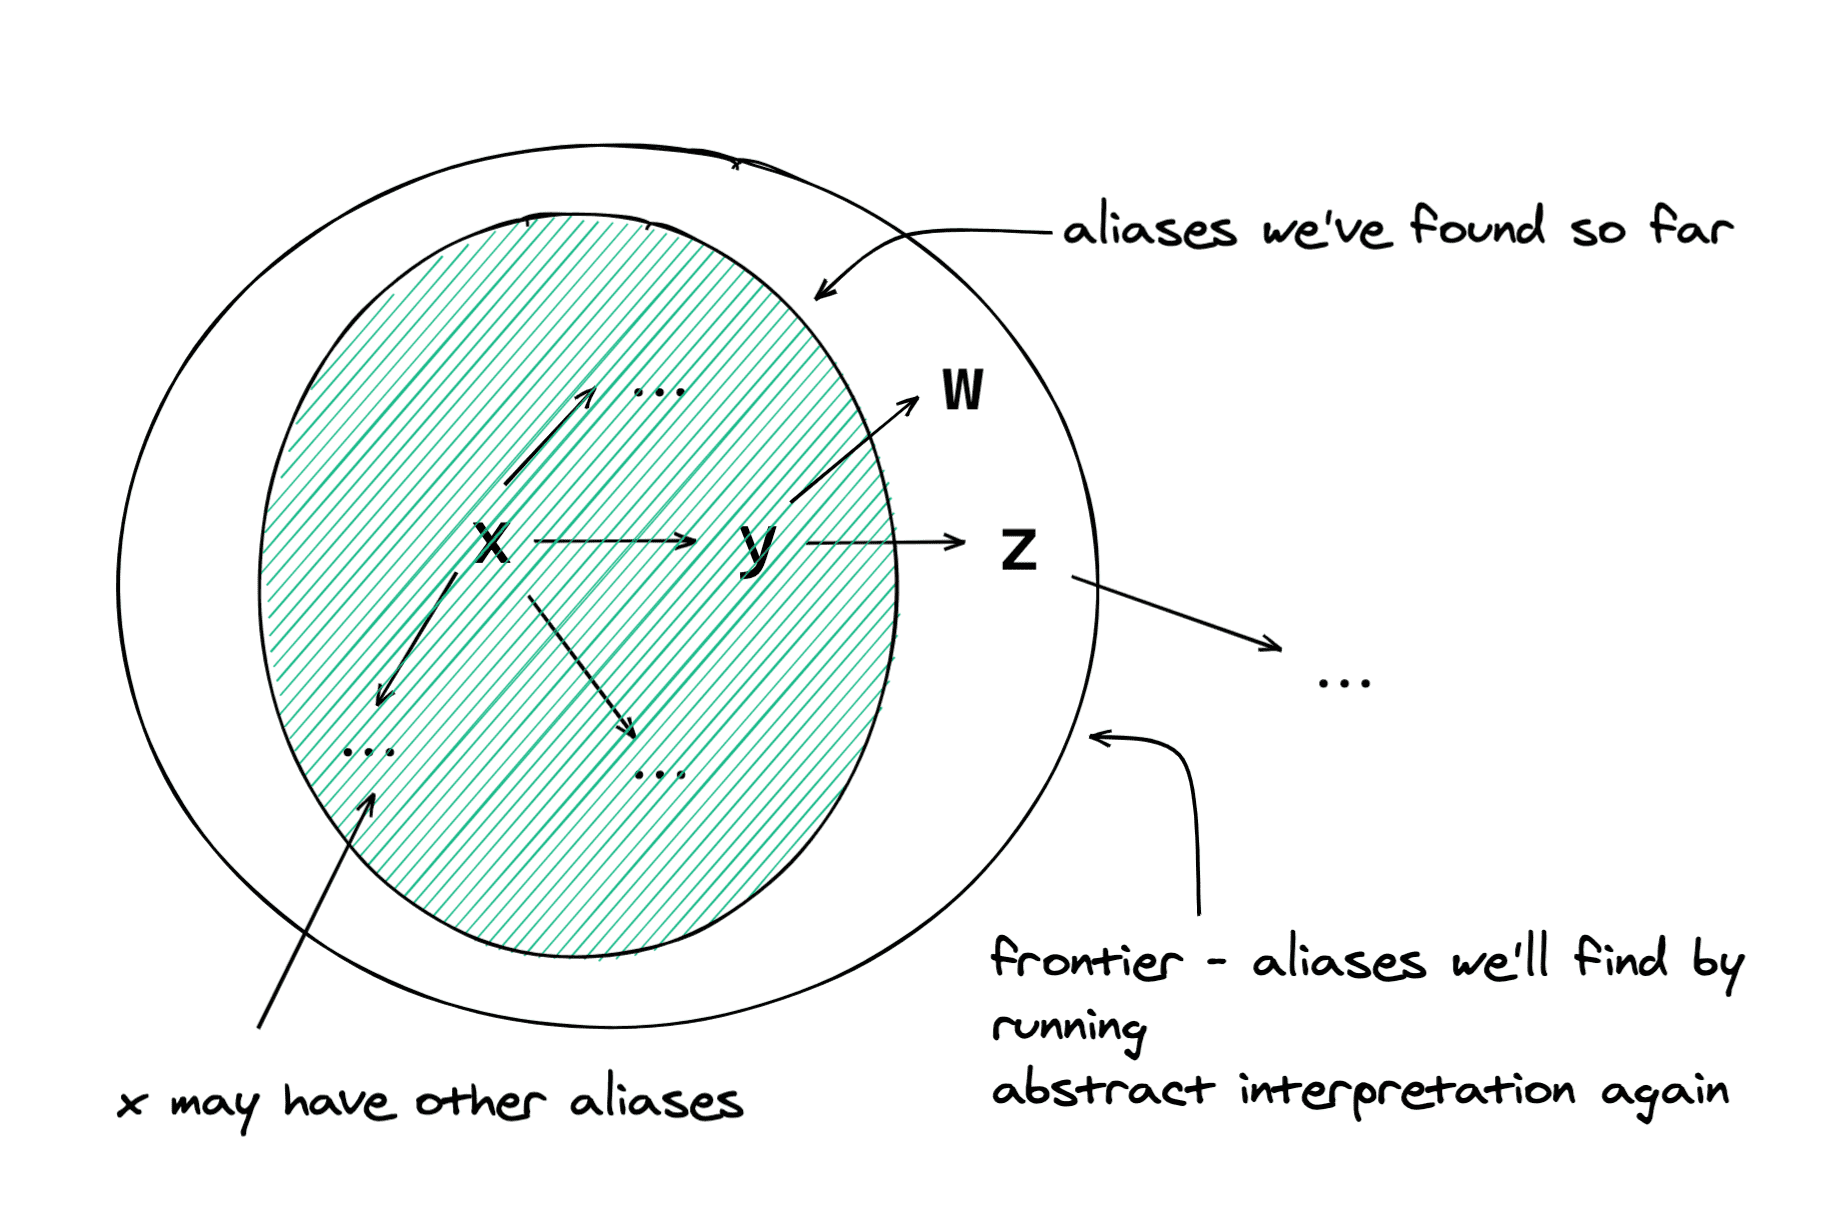
\includegraphics[width=\linewidth]{05_files/alias-frontier.png}} }

So we repeat, until we find no more aliases. The full code is linked in
the repo, and includes an option of matching fields (i.e. should we
consider aliases of \texttt{x.f} as well as \texttt{x}?) We won't in
this case, but other aspects of Bolt's data-race type-checker do use
this.

But the beauty of functional programming is that the function says what
we're doing with no boilerplate:

%{
%\href{https://github.com/mukul-rathi/bolt/blob/master/src/frontend/data_race_checker/data_race_checker_env.ml}{data\_race\_checker\_env.ml}}
%
%Copy

\begin{lstlisting}[language=caml]
let rec get_all_obj_aliases should_match_fields curr_aliases block_expr =
    find_immediate_aliases_in_block_expr should_match_fields name_to_match curr_aliases
      block_expr
    |> fun updated_aliases ->
    if var_lists_are_equal updated_aliases curr_aliases
       then curr_aliases (* we're done! *)
    else get_all_obj_aliases should_match_fields updated_aliases block_expr
    (* repeat with an expanded frontier *)
\end{lstlisting}

\hypertarget{liveness-analysis}{%
\section{\texorpdfstring{\protect\hyperlink{liveness-analysis}{}Liveness
Analysis}{Liveness Analysis}}\label{liveness-analysis}}

Alright, so we're halfway there - we've identified our aliases, now we
need to find out when they're live. Remember a value is \emph{live} if
there's some program execution path in the future it will be used on.

\hypertarget{control-flow-graph}{%
\subsection{\texorpdfstring{\protect\hyperlink{control-flow-graph}{}Control
Flow Graph}{Control Flow Graph}}\label{control-flow-graph}}

To do this, let's formalise the notion of ``execution paths'' in a
program. We're going to be representing a program as a graph of
instructions, with edges representing the steps in the execution. We
call this the \textbf{Control Flow Graph} of the program.

However, if every statement represented a node on the graph, with edges
between them, the graph would be incredibly large (a 100 line program
would have 100 statements). We can be a bit cleverer and group together
statements that will always execute right after each other.

If there's only \textbf{one path} from the start statement to the end
statement in a group of statements, we can represent this as a
\textbf{single node} in our control flow graph. We call this node a
\textbf{basic block} of statements. Below you can see the lines of code
highlighted in different colours to show which basic block they lie in.

\begin{figure}
\centering
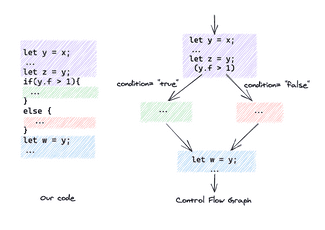
\includegraphics[width=\linewidth]{05_files/control-flow-graph.png}
\caption{Note how the control flow graph shows two different execution
paths, corresponding to the if-else branch taken.}
\end{figure}

In our graph, we can pick any statement in the program and ask, is the
value of variable \texttt{y} live at this point?

A naive way of checking this is to traverse the graph forwards until you
see a use of this value of \texttt{y} (so \texttt{y} is live) or until
you reach the end (you therefore know \texttt{y} is dead). But this is
hopelessly wasteful - for every statement we have to go forward and
traverse the graph to check if the variable's are used.

We can look at it another way, if we traverse \emph{backwards}, then the
first use of \texttt{y} that we encounter is the last use if we
traversed it going forwards. So as soon as we see \texttt{y} being used
when we go backwards, we know that whilst \texttt{y} is defined, it is
live.

A picture helps so let's look at our graph:

{
\href{https://mukulrathi.com/static/12ada8741740841a048f22702b12b7f9/5b503/liveness-range.png}{{}
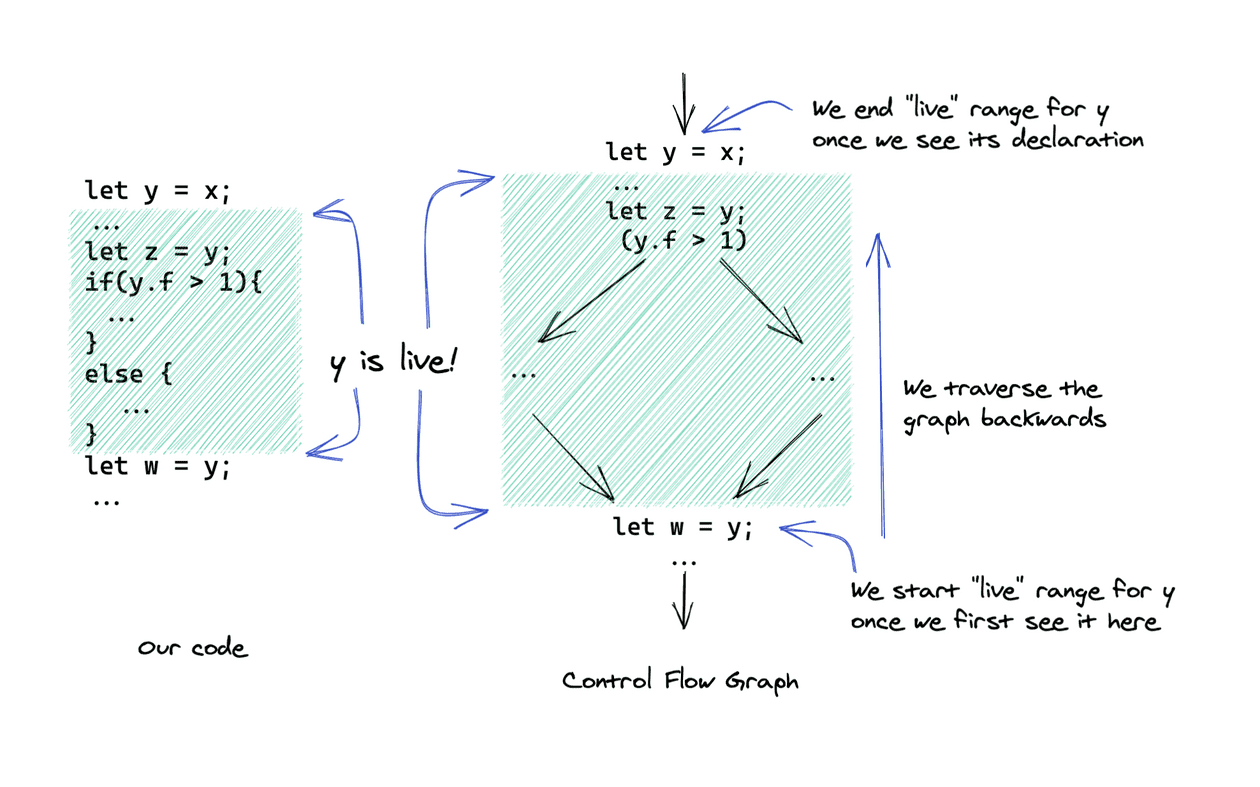
\includegraphics[width=\linewidth]{05_files/liveness-range.png}} }

So to summarise, in liveness analysis we:

\begin{itemize}
\tightlist
\item
  Traverse the Control Flow Graph backwards
\item
  Keep track of the set of live values
\item
  If we see a value for the first time, we add it to our set
\item
  We remove a value if we see its definition
\end{itemize}

\hypertarget{implementing-our-alias-liveness-checker}{%
\section{\texorpdfstring{\protect\hyperlink{implementing-our-alias-liveness-checker}{}Implementing
Our Alias Liveness
Checker}{Implementing Our Alias Liveness Checker}}\label{implementing-our-alias-liveness-checker}}

Now we have our theoretical understanding in place, let's implement the
checker.
%
Whenever we encounter an identifier, we need to know what the original
object reference was, the set of possible aliases, and separately those
that are live.

%{
%\href{https://github.com/mukul-rathi/bolt/blob/master/src/frontend/data_race_checker/type_alias_liveness.ml}{type\_alias\_liveness.ml}}
%
%Copy

\begin{lstlisting}[caption={type\_alias\_liveness.ml},language=caml]
let type_alias_liveness_identifier obj_name possible_aliases
  filter_linear_caps_fn live_aliases id =
  let id_name = get_identifier_name id in
\end{lstlisting}

Our function deals with three cases depending on the identifier name:

\begin{itemize}
\tightlist
\item
  It is the original object reference
\item
  It is a possible alias
\item
  It is another reference we don't care about
\end{itemize}

In the first case, we want to filter the linear capabilities (since the
reference is not linear so can't use them) if there are live aliases.
Along with the updated identifier, we also return the unchanged set of
live aliases.

\begin{lstlisting}[caption={type\_alias\_liveness.ml},language=caml]
if id_name = obj_name then (* original object reference *)
    let maybe_updated_capabilities =
      update_capabilities_if_live_aliases filter_linear_caps_fn
      live_aliases (get_identifier_capabilities id) in
    (set_identifier_capabilities id maybe_updated_capabilities, live_aliases)
\end{lstlisting}


Otherwise, we need to check if the identifier is one of the possible
aliases - if so we add it to the set of live aliases we are tracking. So
we then return this updated set of live aliases along with the
identifier.

%{
%\href{https://github.com/mukul-rathi/bolt/blob/master/src/frontend/data_race_checker/type_alias_liveness.ml}{type\_alias\_liveness.ml}}
%
%Copy


\begin{lstlisting}[language=caml]
else
  ( match
      List.find
        ~f:(fun poss_alias ->
                identifier_matches_var_name poss_alias id)
        possible_aliases
    with
  | Some alias -> alias :: live_aliases
  | None       -> live_aliases )
  |> fun updated_live_aliases -> (id, updated_live_aliases)
\end{lstlisting}

And the dual in our \texttt{type\_alias\_liveness\_expr} function is
when we see our \texttt{let\ x\ =\ e} expression. Here, remember we
execute \texttt{e} first, and then assign it to \texttt{x}, so when
traversing this backwards, we remove \texttt{x} from the set of live
aliases first (since we've seen its definition), \emph{then} we traverse
the bound expression:

\begin{lstlisting}[language=caml]
| Let (loc, type_expr, var_name, bound_expr) ->
      (* remove this var from the set of live aliases *)
      type_alias_liveness_expr_rec
        (List.filter ~f:(fun name -> not (var_name = name)) live_aliases)
        bound_expr
      |> fun (updated_bound_expr, updated_live_aliases) ->
      (Let (loc, type_expr, var_name, updated_bound_expr), updated_live_aliases)
\end{lstlisting}


One interesting case in our Control Flow Graph is the \texttt{if-else}
split. We treat each branch independently of each other, since they are
independent paths in our graph.

\begin{lstlisting}[language=caml]
| If (loc, type_expr, cond_expr, then_expr, else_expr) ->
      type_alias_liveness_block_expr_rec live_aliases then_expr
      |> fun (updated_then_expr, then_live_aliases) ->
      type_alias_liveness_block_expr_rec live_aliases else_expr
      |> fun (updated_else_expr, else_live_aliases) ->
\end{lstlisting}

How do we recombine the two branches? Well, the definition of liveness
is if there is \emph{some} path in which the value is used. Again, we
don't know which branch is taken, because we can't execute the program,
so we \emph{over-approximate} - we assume both paths could have been
taken - so \emph{union} their sets of live aliases, when traversing the
if-else condition expression:

\begin{lstlisting}[language=caml]
type_alias_liveness_expr_rec (then_live_aliases @ else_live_aliases) cond_expr
      |> fun (updated_cond_expr, cond_live_aliases) ->
      ( If (loc, type_expr, updated_cond_expr, updated_then_expr, updated_else_expr)
      , cond_live_aliases )
\end{lstlisting}

Another interesting case is when we have a while loop. We can't just
traverse the loop once, since we might miss out on some values that
could be used in a subsequent iteration and therefore are live. We don't
know how many times we'll go round the loop so as ever we
\emph{over-approximate} - we'll keep going round the loop until the set
of live aliases doesn't change (i.e. we've got all possible live
aliases):
\begin{lstlisting}[language=caml]
and type_alias_liveness_loop_expr aliased_obj_name possible_aliases
  filter_linear_caps_fn live_aliases loop_expr =
  type_alias_liveness_block_expr aliased_obj_name possible_aliases filter_linear_caps_fn
    live_aliases loop_expr
  |> fun (updated_loop_expr, updated_live_aliases) ->
  if var_lists_are_equal live_aliases updated_live_aliases then
     (* done! *)
    (updated_loop_expr, updated_live_aliases)
  else
  (* loop again! *)
    type_alias_liveness_loop_expr aliased_obj_name possible_aliases
      filter_linear_caps_fn updated_live_aliases updated_loop_expr
\end{lstlisting}

%\hypertarget{i-make-content-about-my-software-engineering-journey-curated-in-my-newsletter}{%
%\subsection{I make content about my software engineering journey,
%curated in my
%newsletter!}\label{i-make-content-about-my-software-engineering-journey-curated-in-my-newsletter}}
%
%Tips from my time at Cambridge and Facebook, and early access to
%technical tutorials on machine learning, compilers and beyond.
%
%\href{https://newsletter.mukulrathi.com/}{Check out previous issues!}
%
%Email Address
%
%By subscribing, you agree with Revue's
%\href{https://www.getrevue.co/terms}{Terms of Service} and
%\href{https://www.getrevue.co/privacy}{Privacy Policy}.

\hypertarget{where-does-this-fit-into-bolt}{%
\section{\texorpdfstring{\protect\hyperlink{where-does-this-fit-into-bolt}{}Where
does this fit into
Bolt?}{Where does this fit into Bolt?}}\label{where-does-this-fit-into-bolt}}

Our liveness analysis fits into the overall type-checking for linear
capabilities in Bolt's data-race type-checker:

%{
%\href{https://github.com/mukul-rathi/bolt/blob/master/src/frontend/data_race_checker/type_linear_capabilities.ml}{type\_linear\_capabilities.ml}}
%
%Copy

\begin{lstlisting}[language=caml,caption={type\_linear\_capabilities.ml}]
let type_linear_object_references obj_name obj_class class_defns block_expr =
  let obj_aliases = ...
  ...
  |> fun updated_block_expr ->
  type_alias_liveness_block_expr obj_name obj_aliases
     filter_linear_caps_fn [] (* we start with empty set of live aliases *)
     updated_block_expr
  |> fun (typed_linear_obj_ref_block_expr, _) -> typed_linear_obj_ref_block_expr
\end{lstlisting}

We'll talk more about the other aspects of data-race type-checking
later, however the next stage of the tutorial is on \emph{desugaring} -
the process of taking our high-level language and simplifying it to a
lower-level representation. This will set us up nicely for targeting
LLVM later in the compiler series.

%\hypertarget{share-this-on-twitter}{%
%\subsection{Share This On Twitter}\label{share-this-on-twitter}}
%
%If you liked this post, please consider sharing it with your network. If
%you have any questions, tweet away and I'll answer :) I also tweet when
%new posts drop!
%
%\textbf{PS:} I also share helpful tips and links as I'm learning - so
%you get them \textbf{well before} they make their way into a post!
%
%\includegraphics[width=1.04167in,height=1.11458in]{05_files/profile-pic.png}
%
%\hypertarget{series-creating-the-bolt-compiler-1}{%
%\section{Series: Creating the Bolt
%Compiler}\label{series-creating-the-bolt-compiler-1}}
%
%\begin{itemize}
%\item
%  { Part 1:
%  }\href{https://mukulrathi.com/create-your-own-programming-language/intro-to-compiler/}{How
%  I wrote my own "proper" programming language}
%\item
%  { Part 2:
%  }\href{https://mukulrathi.com/create-your-own-programming-language/compiler-engineering-structure/}{So
%  how do you structure a compiler project?}
%\item
%  { Part 3:
%  }\href{https://mukulrathi.com/create-your-own-programming-language/parsing-ocamllex-menhir/}{Writing
%  a Lexer and Parser using OCamllex and Menhir}
%\item
%  { Part 4:
%  }\href{https://mukulrathi.com/create-your-own-programming-language/intro-to-type-checking/}{An
%  accessible introduction to type theory and implementing a
%  type-checker}
%\item
%  \textbf{Part 5: A tutorial on liveness and alias dataflow analysis}
%\item
%  { Part 6:
%  }\href{https://mukulrathi.com/create-your-own-programming-language/lower-language-constructs-to-llvm/}{Desugaring
%  - taking our high-level language and simplifying it!}
%\item
%  { Part 7:
%  }\href{https://mukulrathi.com/create-your-own-programming-language/protobuf-ocaml-cpp-tutorial/}{A
%  Protobuf tutorial for OCaml and C++}
%\item
%  { Part 8:
%  }\href{https://mukulrathi.com/create-your-own-programming-language/llvm-ir-cpp-api-tutorial/}{A
%  Complete Guide to LLVM for Programming Language Creators}
%\item
%  { Part 9:
%  }\href{https://mukulrathi.com/create-your-own-programming-language/concurrency-runtime-language-tutorial/}{Implementing
%  Concurrency and our Runtime Library}
%\item
%  { Part 10:
%  }\href{https://mukulrathi.com/create-your-own-programming-language/generics-parametric-polymorphism/}{Generics
%  - adding polymorphism to Bolt}
%\item
%  { Part 11:
%  }\href{https://mukulrathi.com/create-your-own-programming-language/inheritance-method-overriding-vtable/}{Adding
%  Inheritance and Method Overriding to Our Language}
%\end{itemize}
%
%\begin{itemize}
%\item ~
%  \hypertarget{an-accessible-introduction-to-type-theory-and-implementing-a-type-checker}{%
%  \subsection{\texorpdfstring{\href{https://mukulrathi.com/create-your-own-programming-language/intro-to-type-checking/}{←
%  An accessible introduction to type theory and implementing a
%  type-checker}}{← An accessible introduction to type theory and implementing a type-checker}}\label{an-accessible-introduction-to-type-theory-and-implementing-a-type-checker}}
%\item ~
%  \hypertarget{desugaring---taking-our-high-level-language-and-simplifying-it}{%
%  \subsection{\texorpdfstring{\href{https://mukulrathi.com/create-your-own-programming-language/lower-language-constructs-to-llvm/}{Desugaring
%  - taking our high-level language and simplifying it!
%  →}}{Desugaring - taking our high-level language and simplifying it! →}}\label{desugaring---taking-our-high-level-language-and-simplifying-it}}
%\end{itemize}
%
%\hypertarget{table-of-contents}{%
%\section{Table of Contents}\label{table-of-contents}}
%
%\href{https://mukulrathi.com/create-your-own-programming-language/data-race-dataflow-analysis/\#top-of-page}{}
%
%\hypertarget{a-tutorial-on-liveness-and-alias-dataflow-analysis}{%
%\subsection{A tutorial on liveness and alias dataflow
%analysis}\label{a-tutorial-on-liveness-and-alias-dataflow-analysis}}
%
%\begin{itemize}
%\item
%  \href{https://mukulrathi.com/create-your-own-programming-language/data-race-dataflow-analysis/\#dataflow-analysis---the-big-picture}{}
%
%  \hypertarget{dataflow-analysis---the-big-picture-1}{%
%  \subsection{Dataflow Analysis - the big
%  picture}\label{dataflow-analysis---the-big-picture-1}}
%\item
%  \href{https://mukulrathi.com/create-your-own-programming-language/data-race-dataflow-analysis/\#alias-analysis}{}
%
%  \hypertarget{alias-analysis-1}{%
%  \subsection{Alias Analysis}\label{alias-analysis-1}}
%
%  \begin{itemize}
%  \item
%    \href{https://mukulrathi.com/create-your-own-programming-language/data-race-dataflow-analysis/\#abstract-interpretation}{}
%
%    \hypertarget{abstract-interpretation-1}{%
%    \subsection{Abstract
%    Interpretation}\label{abstract-interpretation-1}}
%  \item
%    \href{https://mukulrathi.com/create-your-own-programming-language/data-race-dataflow-analysis/\#computing-all-aliases}{}
%
%    \hypertarget{computing-all-aliases-1}{%
%    \subsection{Computing all
%    aliases}\label{computing-all-aliases-1}}
%  \end{itemize}
%\item
%  \href{https://mukulrathi.com/create-your-own-programming-language/data-race-dataflow-analysis/\#liveness-analysis}{}
%
%  \hypertarget{liveness-analysis-1}{%
%  \subsection{Liveness Analysis}\label{liveness-analysis-1}}
%
%  \begin{itemize}
%  \item
%    \href{https://mukulrathi.com/create-your-own-programming-language/data-race-dataflow-analysis/\#control-flow-graph}{}
%
%    \hypertarget{control-flow-graph-1}{%
%    \subsection{Control Flow Graph}\label{control-flow-graph-1}}
%  \end{itemize}
%\item
%  \href{https://mukulrathi.com/create-your-own-programming-language/data-race-dataflow-analysis/\#implementing-our-alias-liveness-checker}{}
%
%  \hypertarget{implementing-our-alias-liveness-checker-1}{%
%  \subsection{Implementing Our Alias Liveness
%  Checker}\label{implementing-our-alias-liveness-checker-1}}
%\item
%  \href{https://mukulrathi.com/create-your-own-programming-language/data-race-dataflow-analysis/\#where-does-this-fit-into-bolt}{}
%
%  \hypertarget{where-does-this-fit-into-bolt-1}{%
%  \subsection{Where does this fit into
%  Bolt?}\label{where-does-this-fit-into-bolt-1}}
%\end{itemize}
%
%© Mukul Rathi 2023
%
%\hypertarget{gatsby-announcer}{}
%Navigated to A tutorial on liveness and alias dataflow analysis

%\hypertarget{___gatsby}{}
%\hypertarget{gatsby-focus-wrapper}{}
%\href{https://mukulrathi.com/}{}
%
%MUKUL RATHI
%
%\href{https://mukulrathi.com/about-me}{}
%
%About Me
%
%\href{https://mukulrathi.com/blog}{}
%
%Blog
%
%\hypertarget{creating-the-bolt-compiler-part-6}{%
%\subsection{Creating the Bolt Compiler: Part
%6}\label{creating-the-bolt-compiler-part-6}}

\hypertarget{top-of-page}{%
\chapter{Desugaring - taking our high-level language and simplifying
it!}\label{top-of-page}}

July 01, 2020

%\hypertarget{july-01-2020}{%
%\subsection{July 01, 2020}\label{july-01-2020}}
%
%\hypertarget{min-read}{%
%\subsection{6 min read}\label{min-read}}

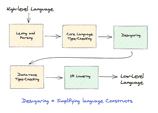
\includegraphics[width=\linewidth]{06_files/desugaring.png}

%\hypertarget{series-creating-the-bolt-compiler}{%
%\section{Series: Creating the Bolt
%Compiler}\label{series-creating-the-bolt-compiler}}
%
%\begin{itemize}
%\item
%  { Part 1:
%  }\href{https://mukulrathi.com/create-your-own-programming-language/intro-to-compiler/}{How
%  I wrote my own "proper" programming language}
%\item
%  { Part 2:
%  }\href{https://mukulrathi.com/create-your-own-programming-language/compiler-engineering-structure/}{So
%  how do you structure a compiler project?}
%\item
%  { Part 3:
%  }\href{https://mukulrathi.com/create-your-own-programming-language/parsing-ocamllex-menhir/}{Writing
%  a Lexer and Parser using OCamllex and Menhir}
%\item
%  { Part 4:
%  }\href{https://mukulrathi.com/create-your-own-programming-language/intro-to-type-checking/}{An
%  accessible introduction to type theory and implementing a
%  type-checker}
%\item
%  { Part 5:
%  }\href{https://mukulrathi.com/create-your-own-programming-language/data-race-dataflow-analysis/}{A
%  tutorial on liveness and alias dataflow analysis}
%\item
%  \textbf{Part 6: Desugaring - taking our high-level language and
%  simplifying it!}
%\item
%  { Part 7:
%  }\href{https://mukulrathi.com/create-your-own-programming-language/protobuf-ocaml-cpp-tutorial/}{A
%  Protobuf tutorial for OCaml and C++}
%\item
%  { Part 8:
%  }\href{https://mukulrathi.com/create-your-own-programming-language/llvm-ir-cpp-api-tutorial/}{A
%  Complete Guide to LLVM for Programming Language Creators}
%\item
%  { Part 9:
%  }\href{https://mukulrathi.com/create-your-own-programming-language/concurrency-runtime-language-tutorial/}{Implementing
%  Concurrency and our Runtime Library}
%\item
%  { Part 10:
%  }\href{https://mukulrathi.com/create-your-own-programming-language/generics-parametric-polymorphism/}{Generics
%  - adding polymorphism to Bolt}
%\item
%  { Part 11:
%  }\href{https://mukulrathi.com/create-your-own-programming-language/inheritance-method-overriding-vtable/}{Adding
%  Inheritance and Method Overriding to Our Language}
%\end{itemize}
%
%\begin{center}\rule{0.5\linewidth}{0.5pt}\end{center}

\hypertarget{just-give-me-the-code}{%
\section{\texorpdfstring{\protect\hyperlink{just-give-me-the-code}{}Just
give me the
code!}{Just give me the code!}}\label{just-give-me-the-code}}

All the illustrative code snippets in this blog post link to the
respective file in the \href{https://github.com/mukul-rathi/bolt}{Bolt
repository}. There's more code in there than could be covered without
making this post extremely long!

The first half of this post will be looking at the
\href{https://github.com/mukul-rathi/bolt/tree/master/src/frontend/desugaring}{desugaring/
folder} and the second half is covering the
\href{https://github.com/mukul-rathi/bolt/tree/master/src/frontend/ir_gen}{ir\_gen/
folder}.

\hypertarget{what-is-desugaring}{%
\section{\texorpdfstring{\protect\hyperlink{what-is-desugaring}{}What
is desugaring?}{What is desugaring?}}\label{what-is-desugaring}}

Programming languages are a series of abstractions. No one writes
programs by typing in 0s and 1s - it's just not human readable. The
closest we get to the hardware operations is with \textbf{assembly code}
e.g. series of \texttt{add} \texttt{mov} and \texttt{jmp} instructions.

Assembly code is still not really a pleasant programming experience.
Even languages we deem as \emph{low-level} like C / C++ / Rust offer a
host of abstractions over assembly code - things you take for granted
like \texttt{if} statements and \texttt{while} loops.

We call these abstractions \textbf{syntactic sugar} - named because they
make it \emph{sweeter} for programmers to program in that language.

When we're writing a compiler though, we're going the other way - we're
\emph{desugaring} the source code - stripping away higher-level
constructs. We also refer to this as \emph{lowering} the high-level
language constructs.

In this post we'll start by looking at desugaring a for loop. We'll then
look at the ``Desugaring'' and ``IR Lowering'' stages in the Bolt
compiler frontend. This will wrap up our compiler frontend and set us up
to switch to C++ for the compiler backend.

\hypertarget{desugaring-for-loops}{%
\section{\texorpdfstring{\protect\hyperlink{desugaring-for-loops}{}Desugaring
For Loops}{Desugaring For Loops}}\label{desugaring-for-loops}}

The first case we desugar is actually between the parsing and
type-checking phases - desugaring a \texttt{for} loop into a while loop:

{desugar\_for\_loop.bolt}

Copy

\begin{verbatim}
for (let i = 0; i < n; i:=i+1) {  doSomething}
// desugared
let i = 0;while (i < n) {  doSomething;  i:=i+1}
\end{verbatim}

Note we handle this as a special case when type-checking the expression,
however you might imagine if there was more sugar (like \texttt{++i}
instead of \texttt{i:=i+1}) that we might add a full desugaring stage
between the parsed AST and typed AST:

\begin{lstlisting}[language=caml,caption={type\_expr.ml}]
let rec type_expr class_defns function_defns (expr : Parsed_ast.expr) env =
...
| Parsed_ast.For
      (loc, start_expr, cond_expr, step_expr, Parsed_ast.Block (block_loc, loop_expr)) ->
      (* desugar into a while loop *)
      type_block_with_defns
        (Parsed_ast.Block
           ( loc
           , [ start_expr
             ; Parsed_ast.While
                 (loc, cond_expr,
                 Parsed_ast.Block (block_loc, loop_expr @ [step_expr]))
             ] ))
        env
\end{lstlisting}
\hypertarget{desugaring-between-type-checking-stages}{%
\section{\texorpdfstring{\protect\hyperlink{desugaring-between-type-checking-stages}{}Desugaring
between type-checking
stages}{Desugaring between type-checking stages}}\label{desugaring-between-type-checking-stages}}

Desugaring gets its own stage in between the two stages of
type-checking. The data-race type-checking is much more complex than the
traditional type-checking (\texttt{int}, \texttt{bool} etc), so we
simplify the language to \emph{avoid having to consider as many cases}.

\hypertarget{removing-variable-shadowing}{%
\subsection{\texorpdfstring{\protect\hyperlink{removing-variable-shadowing}{}Removing
variable
shadowing}{Removing variable shadowing}}\label{removing-variable-shadowing}}

For example, consider variable shadowing, where we can declare the same
variable name \texttt{x} in nested scopes: Consider the following:

%{variable\_shadowing.bolt}
%
%Copy

\begin{verbatim}
let x = 0;
if (x >= 0) {
  let x = 1;
  let y = x + 1
 // we now refer to the value x=1}
else {
 // we refer to the value x=0 
x := 1
}
\end{verbatim}

Variable shadowing is syntactic sugar - we don't require the programmer
to use unique variable names in nested scopes. It makes the
{alias
liveness analysis previously discussed} much harder. How do we know
which value of x is being aliased? We could track which scope we're in
\emph{orrrr} we could avoid it. It's much easier to deal with once we
give variables unique names:

%{unique\_variable\_names.bolt}
%
%Copy

\begin{verbatim}
let _x0 = 0;
if (_x0 >= 0) {
  let _x1 = 1;
  let y = _x1+ 1
} else { _x0 := 1}
\end{verbatim}

We first create a mapping from old to new variable names. We count the
number of times the variable has been declared so far in outer scopes
and stick that count on the end of the variable name. And to specify
that these are compiler-generated names we prepend them with an
\texttt{\_}, since in Bolt programmers can't define a variable starting
with an \texttt{\_}.

\begin{lstlisting}[language=caml,caption={{remove\_variable\_shadowing.ml}}]
type var_name_map = (Var_name.t * Var_name.t) list

let set_unique_name var_name var_name_map =
  let num_times_var_declared =
    List.length (List.filter ~f:(fun (name, _) -> name = var_name) var_name_map) in
  Var_name.of_string
    (Fmt.str "_%s%d" (Var_name.to_string var_name) num_times_var_declared)
\end{lstlisting}


\hypertarget{desugaring-function--method-overloading}{%
\subsection{\texorpdfstring{\protect\hyperlink{desugaring-function--method-overloading}{}Desugaring
Function / Method
Overloading}{Desugaring Function / Method Overloading}}\label{desugaring-function--method-overloading}}

Function overloading is where we define multiple functions with the
\emph{same} name but \emph{different} parameter types. This is useful if
you want to call a different \texttt{print} method based on the type of
the arguments passed in:

%{function\_overloading.bolt}
%
%Copy

\begin{verbatim}
function void print(Foo x){  ...}
function void print(Bar x){  ...}
function void print(int x){  ...}
\end{verbatim}

Again, this is a nice-to-have construct, but we've got an issue - which
function do we call? We can't tell from the source code, but we can use
the information about the argument types from the previous type-checking
stage.

By desugaring more complex language constructs to simpler language
constructs, we make subsequent stages of the compiler simpler - they
\textbf{do not need to know} about anything that has been desugared.

We encode the type of the parameters in the function application
expression when type-checking it:

\begin{lstlisting}[language=caml,caption={type\_expr.ml}]
| Parsed_ast.FunctionApp (loc, func_name, args_exprs) ->
      type_args type_with_defns args_exprs env
      >>= fun (typed_args_exprs, args_types) ->
      get_matching_function_type class_defns func_name args_types function_defns loc
      >>| fun (param_types, return_type) ->
      ( Typed_ast.FunctionApp (loc, return_type, param_types, func_name, typed_args_exprs)
      , return_type )
\end{lstlisting}

\hypertarget{name-mangling-functions}{%
\paragraph{\texorpdfstring{\protect\hyperlink{name-mangling-functions}{}Name
mangling
functions}{Name mangling functions}}\label{name-mangling-functions}}

Now since each overloaded function has differing parameter types, we can
map the parameter types to a unique string, which we append onto our
function name. We call this process of generating a unique function name
\textbf{name mangling}.

We're going to take the approach used in C++.

For each of the primitive types, we can map them to a unique single
character, whilst for classes we map them to the class name prepended
with its length. We then concatenate all param types together.

Why prepend the length? Consider param types \texttt{(Foo\ x,\ Bar\ y)}
and \texttt{(FooBar\ x)} - both would map to \texttt{FooBar} if we
concatenated their parameter names. Only when we prepend the lengths can
they be distinguished - \texttt{3Foo3Bar} vs \texttt{6FooBar}.
%
%{
%\href{https://github.com/mukul-rathi/bolt/blob/master/src/frontend/desugaring/desugar_overloading.ml}{desugar\_overloading.ml}}
%
%Copy

\begin{lstlisting}[caption={desugar\_overloading.ml},language=caml]
let name_mangle_param_types param_types =
  String.concat
    (List.map
       ~f:(function
         | TEVoid                  -> "v"
         | TEInt                   -> "i"
         | TEBool                  -> "b"
         | TEClass (class_name, _) ->
             let class_name_str = Class_name.to_string class_name in
             Fmt.str "%d%s" (String.length class_name_str) class_name_str)
       param_types)
\end{lstlisting}

%\begin{verbatim}
%let name_mangle_param_types param_types =  String.concat    (List.map       ~f:(function         | TEVoid                  -> "v"         | TEInt                   -> "i"         | TEBool                  -> "b"         | TEClass (class_name, _) ->             let class_name_str = Class_name.to_string class_name in             Fmt.str "%d%s" (String.length class_name_str) class_name_str)       param_types)
%\end{verbatim}

And then to name mangle a method or function, we have the following
code:

\begin{lstlisting}[caption={desugar\_overloading.ml},language=caml]
let name_mangle_overloaded_method meth_name param_types =
  Method_name.of_string
    (Fmt.str "_%s%s"
       (Method_name.to_string meth_name)
       (name_mangle_param_types param_types))
\end{lstlisting}

For example, with this name mangling scheme,
\texttt{testFun(Foo\ x,\ Bar\ y)} maps to
\texttt{\_testFun3Foo3Bar(Foo\ x,\ Bar\ y)}.

If you look at the master branch of the Bolt repo, you'll notice the
desugaring stage also desugars generics. That's a topic that deserves
its own post later in the series!

\hypertarget{lowering-to-ir}{%
\section{\texorpdfstring{\protect\hyperlink{lowering-to-ir}{}Lowering
to IR}{Lowering to IR}}\label{lowering-to-ir}}

Recapping so far, we first looked at desugaring for loops - this occurs
between the parsing and first stage of type-checking. We then looked at
the desugaring stage which sits between the two stages of type-checking.
We now look at IR lowering stage that occurs after type-checking.

IR stands for \emph{intermediate representation} - it is simpler than
the source code, but not quite lowered all the way down to assembly
code.

Our goal with this IR is to \textbf{get close to the LLVM
representation}, to make working with the LLVM API as simple as
possible. We'll also strip away any unnecessary information that we
won't need when running the program.

%\hypertarget{i-make-content-about-my-software-engineering-journey-curated-in-my-newsletter}{%
%\subsection{I make content about my software engineering journey,
%curated in my
%newsletter!}\label{i-make-content-about-my-software-engineering-journey-curated-in-my-newsletter}}
%
%Tips from my time at Cambridge and Facebook, and early access to
%technical tutorials on machine learning, compilers and beyond.
%
%\href{https://newsletter.mukulrathi.com/}{Check out previous issues!}
%
%Email Address
%
%By subscribing, you agree with Revue's
%\href{https://www.getrevue.co/terms}{Terms of Service} and
%\href{https://www.getrevue.co/privacy}{Privacy Policy}.

\hypertarget{lowering-objects-to-structs}{%
\subsection{\texorpdfstring{\protect\hyperlink{lowering-objects-to-structs}{}Lowering
Objects to
Structs}{Lowering Objects to Structs}}\label{lowering-objects-to-structs}}

Classes are an \textbf{abstraction} that group together fields and
methods. LLVM IR doesn't contain classes and objects, only
\textbf{structs}, which are just a group of fields.

{
\href{https://mukulrathi.com/static/a394f0ce0e8ccdc6c4aa56d97ee923b1/7f15f/struct-memory.png}{{}
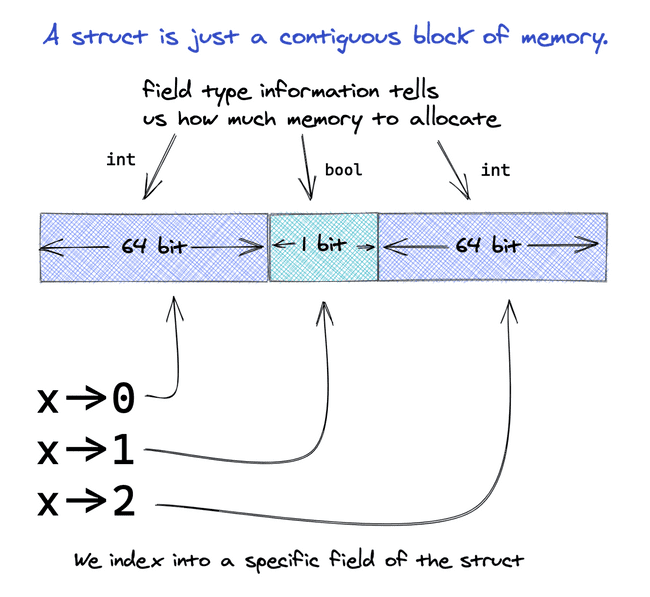
\includegraphics[width=\linewidth]{06_files/struct-memory.png}} }

So how do we map from our Bolt class definition to a struct? We strip
away information from our class:

\begin{itemize}
\tightlist
\item
  We dropped the \texttt{var} / \texttt{const} in the field definitions
\item
  We dropped the capability annotations
\item
  We drop type information in the AST except for field types
\item
  We drop \texttt{loc} (line-position information that we used for our
  type-checker error messages).
\item
  We drop field names
\item
  We no longer associate methods with a class (more on that in a
  second!)
\end{itemize}

Recall, the goal of annotating types and capabilities to our AST is to
check the program is correct. If we can assign a type to an expression,
then it is \emph{well-typed} so it satisfies our notion of correctness.
Likewise, if we can assign capabilities then we know our program doesn't
have data races. And \texttt{const} is just a compiler check to prevent
us reassigning a field.

Once we've checked all that, we can drop that information, since we
don't need it later in the compiler. In fact, our class definition is
now quite barebones - just the class name (a \texttt{string}), and a
list of field types, which LLVM will use to decide how much memory to
allocate to an object:

%{
%\href{https://github.com/mukul-rathi/bolt/blob/master/src/frontend/ir_gen/frontend_ir.mli}{frontend\_ir.mli}}
%
%Copy

\begin{lstlisting}[caption={{frontend\_ir.mli}},language=caml]
type class_defn = TClass of string * type_expr list
\end{lstlisting}

Field names are useful to us as programmers, but for the computer we
don't need to name our fields, we can number them instead as an
\textbf{index} into the struct. Intuitively this is just like array
indices.

%{
%\href{https://github.com/mukul-rathi/bolt/blob/master/src/frontend/ir_gen/ir_gen_env.ml}{ir\_gen\_env.ml}}
%
%Copy

\begin{lstlisting}[caption={{ir\_gen\_env.ml}},language=caml]
let ir_gen_field_index field_name class_name class_defns =
  get_class_fields class_name class_defns
  |> fun field_defns ->
  List.find_mapi_exn
    ~f:(fun index (TField (_, _, name, _)) ->
      if name = field_name then Some index else None)
    field_defns
\end{lstlisting}

%
%\begin{verbatim}
%let ir_gen_field_index field_name class_name class_defns =  get_class_fields class_name class_defns  |> fun field_defns ->  List.find_mapi_exn    ~f:(fun index (TField (_, _, name, _)) ->      if name = field_name then Some index else None)    field_defns
%\end{verbatim}

Note this \texttt{List.find\_mapi\_exn} function name might seem
complex, but the goal is to \texttt{find} the field that matches the
given field name by going through (\texttt{map}) each element of the
list, along with that field's index (hence \texttt{mapi} not
\texttt{map}), and raising an exception (\texttt{exn}) if it is not
found. In practice, this function will never raise an exception because
we already have checked in an earlier type-checking stage that the field
exists.

Methods are just ordinary functions that implicitly take in an
additional parameter: \texttt{this}, which refers to the object that
called the method. In Python, this additional parameter (referred to as
\texttt{self}) is explicitly declared in method declarations.

Note we need to name-mangle our methods again, by prepending the class
name. Right now, we have unique method names \emph{within} a class, when
we separate them as normal functions, they need to be \emph{globally}
uniquely named.

{
\href{https://mukulrathi.com/static/c42e7c83dd7245e132403d79cf89c41e/fa60d/lower-classes.png}{{}
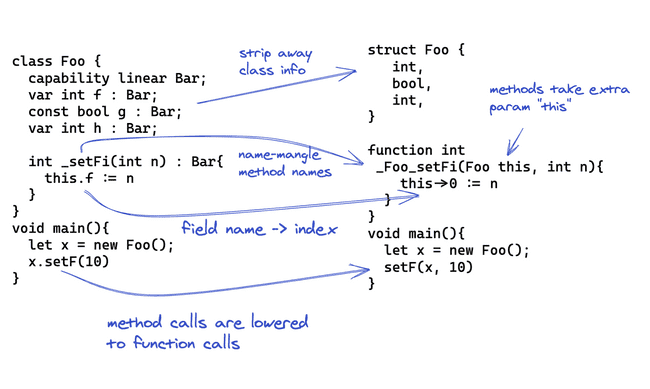
\includegraphics[width=\linewidth]{06_files/lower-classes.png}} }

\hypertarget{automatically-inserting-locks}{%
\subsection{\texorpdfstring{\protect\hyperlink{automatically-inserting-locks}{}Automatically
Inserting
Locks}{Automatically Inserting Locks}}\label{automatically-inserting-locks}}

Bolt has a \texttt{locked} capability, which is similar to the
\texttt{synchronised} keyword in Java - this wraps locks around any
access. Since we're dropping this locked capability we need to specify
lock/unlock instructions in our IR.
%
%{
%\href{https://github.com/mukul-rathi/bolt/blob/master/src/frontend/ir_gen/frontend_ir.mli}{frontend\_ir.mli}}
%
%Copy

\begin{lstlisting}[language=caml,caption={frontend\_ir.mli}]
type lock_type = Reader  | Writer
type expr =  
| Integer     of int  
| Boolean     of bool  
| Identifier  of identifier * lock_type option
  (* maybe acquire a lock when accessing an identifier *) 
 ...  
| Lock        of string * lock_type
  | Unlock    of string * lock_type
\end{lstlisting}

and our to insert locks, we lock the object (\texttt{this}) and then
compute the return value, release the lock and return the value:

%Copy

\begin{verbatim}
... {  methodBody}
// adding locks...
{  lock(this);  
let retVal = methodBody;  
unlock(this);
  retVal}
\end{verbatim}

The corresponding generation code is:

%{
%\href{https://github.com/mukul-rathi/bolt/blob/master/src/frontend/ir_gen/ir_gen_class_and_function_defns.ml}{ir\_gen\_class\_and\_function\_defns.ml}}
%
%Copy

\begin{lstlisting}[language=caml,caption={ir\_gen\_class\_and\_function\_defns.ml}]
let ir_gen_class_method_defn class_defns class_name
    (Desugared_ast.TMethod
       ( method_name
       , _
       (* drop info about whether returning borrowed ref *)
       , return_type
       , params
       , capabilities_used
       , body_expr )) =
    ...
   |> fun ir_body_expr ->
  (* check if we use locked capability *)
  ( match
      List.find
        ~f:(fun (Ast_types.TCapability (mode, _))
        -> mode = Ast_types.Locked)
        capabilities_used
    with
  | Some _lockedCap ->
      [ Frontend_ir.Lock ("this", Frontend_ir.Writer)
      ; Frontend_ir.Let ("retVal", Frontend_ir.Block ir_body_expr)
      ; Frontend_ir.Unlock ("this", Frontend_ir.Writer)
      ; Frontend_ir.Identifier (Frontend_ir.Variable "retVal", None) ]
  | None (* no locks used *) -> ir_body_expr )
  |> fun maybe_locked_ir_body_expr ->
  Frontend_ir.TFunction
    (ir_method_name, ir_return_type, ir_params, maybe_locked_ir_body_expr)
\end{lstlisting}
And for the identifiers, if we're meant to lock them, we acquire a
Reader/Writer Lock depending on whether we're reading from them or
assigning a value to them:

\begin{lstlisting}[language=caml,caption={ir\_gen\_expr.ml}]
let rec ir_gen_expr class_defns expr =
...
  | Desugared_ast.Identifier (_, id) ->
      ir_gen_identifier class_defns id
      |> fun (ir_id, should_lock) ->
      let lock_held = if should_lock then Some Frontend_ir.Reader else None in
      Frontend_ir.Identifier (ir_id, lock_held)
...
  | Desugared_ast.Assign (_, _, id, assigned_expr) ->
      ir_gen_identifier class_defns id
      |> fun (ir_id, should_lock) ->
      ir_gen_expr class_defns assigned_expr
      |> fun ir_assigned_expr ->
      let lock_held = if should_lock then Some Frontend_ir.Writer else None in
      Frontend_ir.Assign (ir_id, ir_assigned_expr, lock_held)
\end{lstlisting}

\hypertarget{wrapping-up-our-compiler-frontend}{%
\section{\texorpdfstring{\protect\hyperlink{wrapping-up-our-compiler-frontend}{}Wrapping
Up Our Compiler
Frontend}{Wrapping Up Our Compiler Frontend}}\label{wrapping-up-our-compiler-frontend}}

As mentioned in the previous parts, the
\href{https://github.com/mukul-rathi/bolt}{Bolt repository} also
contains code for other language features (inheritance and generics,
coming in a later post). So don't worry about ``vtables'' mentioned in
the \texttt{ir\_gen/} folder. To see a simpler version of the repository
before these features were added, run
\texttt{git\ checkout\ simple-compiler-tutorial}.

We've now wrapped up our discussion of the compiler frontend!

Next we're going to be switching from OCaml to C++ for the LLVM IR Code
generation. To do this we'll be using Protobuf, a cross-language binary
serialisation format.

Once we've done that, in a couple of posts we can talk about LLVM's C++
API!

%\hypertarget{share-this-on-twitter}{%
%\subsection{Share This On Twitter}\label{share-this-on-twitter}}
%
%If you liked this post, please consider sharing it with your network. If
%you have any questions, tweet away and I'll answer :) I also tweet when
%new posts drop!
%
%\textbf{PS:} I also share helpful tips and links as I'm learning - so
%you get them \textbf{well before} they make their way into a post!
%
%\hypertarget{series-creating-the-bolt-compiler-1}{%
%\section{Series: Creating the Bolt
%Compiler}\label{series-creating-the-bolt-compiler-1}}
%
%\begin{itemize}
%\item
%  { Part 1:
%  }\href{https://mukulrathi.com/create-your-own-programming-language/intro-to-compiler/}{How
%  I wrote my own "proper" programming language}
%\item
%  { Part 2:
%  }\href{https://mukulrathi.com/create-your-own-programming-language/compiler-engineering-structure/}{So
%  how do you structure a compiler project?}
%\item
%  { Part 3:
%  }\href{https://mukulrathi.com/create-your-own-programming-language/parsing-ocamllex-menhir/}{Writing
%  a Lexer and Parser using OCamllex and Menhir}
%\item
%  { Part 4:
%  }\href{https://mukulrathi.com/create-your-own-programming-language/intro-to-type-checking/}{An
%  accessible introduction to type theory and implementing a
%  type-checker}
%\item
%  { Part 5:
%  }\href{https://mukulrathi.com/create-your-own-programming-language/data-race-dataflow-analysis/}{A
%  tutorial on liveness and alias dataflow analysis}
%\item
%  \textbf{Part 6: Desugaring - taking our high-level language and
%  simplifying it!}
%\item
%  { Part 7:
%  }\href{https://mukulrathi.com/create-your-own-programming-language/protobuf-ocaml-cpp-tutorial/}{A
%  Protobuf tutorial for OCaml and C++}
%\item
%  { Part 8:
%  }\href{https://mukulrathi.com/create-your-own-programming-language/llvm-ir-cpp-api-tutorial/}{A
%  Complete Guide to LLVM for Programming Language Creators}
%\item
%  { Part 9:
%  }\href{https://mukulrathi.com/create-your-own-programming-language/concurrency-runtime-language-tutorial/}{Implementing
%  Concurrency and our Runtime Library}
%\item
%  { Part 10:
%  }\href{https://mukulrathi.com/create-your-own-programming-language/generics-parametric-polymorphism/}{Generics
%  - adding polymorphism to Bolt}
%\item
%  { Part 11:
%  }\href{https://mukulrathi.com/create-your-own-programming-language/inheritance-method-overriding-vtable/}{Adding
%  Inheritance and Method Overriding to Our Language}
%\end{itemize}
%
%\begin{itemize}
%\item ~
%  \hypertarget{a-tutorial-on-liveness-and-alias-dataflow-analysis}{%
%  \subsection{\texorpdfstring{\href{https://mukulrathi.com/create-your-own-programming-language/data-race-dataflow-analysis/}{←
%  A tutorial on liveness and alias dataflow
%  analysis}}{← A tutorial on liveness and alias dataflow analysis}}\label{a-tutorial-on-liveness-and-alias-dataflow-analysis}}
%\item ~
%  \hypertarget{a-protobuf-tutorial-for-ocaml-and-c}{%
%  \subsection{\texorpdfstring{\href{https://mukulrathi.com/create-your-own-programming-language/protobuf-ocaml-cpp-tutorial/}{A
%  Protobuf tutorial for OCaml and C++
%  →}}{A Protobuf tutorial for OCaml and C++ →}}\label{a-protobuf-tutorial-for-ocaml-and-c}}
%\end{itemize}
%
%\hypertarget{table-of-contents}{%
%\section{Table of Contents}\label{table-of-contents}}
%
%\href{https://mukulrathi.com/create-your-own-programming-language/lower-language-constructs-to-llvm/\#top-of-page}{}
%
%\hypertarget{desugaring---taking-our-high-level-language-and-simplifying-it}{%
%\subsection{Desugaring - taking our high-level language and
%simplifying
%it!}\label{desugaring---taking-our-high-level-language-and-simplifying-it}}
%
%\begin{itemize}
%\item
%  \href{https://mukulrathi.com/create-your-own-programming-language/lower-language-constructs-to-llvm/\#just-give-me-the-code}{}
%
%  \hypertarget{just-give-me-the-code-1}{%
%  \subsection{Just give me the code!}\label{just-give-me-the-code-1}}
%\item
%  \href{https://mukulrathi.com/create-your-own-programming-language/lower-language-constructs-to-llvm/\#what-is-desugaring}{}
%
%  \hypertarget{what-is-desugaring-1}{%
%  \subsection{What is desugaring?}\label{what-is-desugaring-1}}
%\item
%  \href{https://mukulrathi.com/create-your-own-programming-language/lower-language-constructs-to-llvm/\#desugaring-for-loops}{}
%
%  \hypertarget{desugaring-for-loops-1}{%
%  \subsection{Desugaring For Loops}\label{desugaring-for-loops-1}}
%\item
%  \href{https://mukulrathi.com/create-your-own-programming-language/lower-language-constructs-to-llvm/\#desugaring-between-type-checking-stages}{}
%
%  \hypertarget{desugaring-between-type-checking-stages-1}{%
%  \subsection{Desugaring between type-checking
%  stages}\label{desugaring-between-type-checking-stages-1}}
%
%  \begin{itemize}
%  \item
%    \href{https://mukulrathi.com/create-your-own-programming-language/lower-language-constructs-to-llvm/\#removing-variable-shadowing}{}
%
%    \hypertarget{removing-variable-shadowing-1}{%
%    \subsection{Removing variable
%    shadowing}\label{removing-variable-shadowing-1}}
%  \item
%    \href{https://mukulrathi.com/create-your-own-programming-language/lower-language-constructs-to-llvm/\#desugaring-function--method-overloading}{}
%
%    \hypertarget{desugaring-function-method-overloading}{%
%    \subsection{Desugaring Function / Method
%    Overloading}\label{desugaring-function-method-overloading}}
%  \end{itemize}
%\item
%  \href{https://mukulrathi.com/create-your-own-programming-language/lower-language-constructs-to-llvm/\#lowering-to-ir}{}
%
%  \hypertarget{lowering-to-ir-1}{%
%  \subsection{Lowering to IR}\label{lowering-to-ir-1}}
%
%  \begin{itemize}
%  \item
%    \href{https://mukulrathi.com/create-your-own-programming-language/lower-language-constructs-to-llvm/\#lowering-objects-to-structs}{}
%
%    \hypertarget{lowering-objects-to-structs-1}{%
%    \subsection{Lowering Objects to
%    Structs}\label{lowering-objects-to-structs-1}}
%  \item
%    \href{https://mukulrathi.com/create-your-own-programming-language/lower-language-constructs-to-llvm/\#automatically-inserting-locks}{}
%
%    \hypertarget{automatically-inserting-locks-1}{%
%    \subsection{Automatically Inserting
%    Locks}\label{automatically-inserting-locks-1}}
%  \end{itemize}
%\item
%  \href{https://mukulrathi.com/create-your-own-programming-language/lower-language-constructs-to-llvm/\#wrapping-up-our-compiler-frontend}{}
%
%  \hypertarget{wrapping-up-our-compiler-frontend-1}{%
%  \subsection{Wrapping Up Our Compiler
%  Frontend}\label{wrapping-up-our-compiler-frontend-1}}
%\end{itemize}
%
%© Mukul Rathi 2023
%
%\hypertarget{gatsby-announcer}{}
%Navigated to Desugaring - taking our high-level language and simplifying
%it!

%\hypertarget{___gatsby}{}
%\hypertarget{gatsby-focus-wrapper}{}
%\href{https://mukulrathi.com/}{}
%
%MUKUL RATHI
%
%\href{https://mukulrathi.com/about-me}{}
%
%About Me
%
%\href{https://mukulrathi.com/blog}{}
%
%Blog
%
%\hypertarget{creating-the-bolt-compiler-part-7}{%
%\section{Creating the Bolt Compiler: Part
%7}\label{creating-the-bolt-compiler-part-7}}

\hypertarget{top-of-page}{%
\chapter{A Protobuf tutorial for OCaml and C++}\label{top-of-page}}

October 03, 2020


\includegraphics[width=\linewidth]{07_files/protobuf.png}

%\hypertarget{october-03-2020}{%
%\section{October 03, 2020}\label{october-03-2020}}
%
%\hypertarget{min-read}{%
%\section{8 min read}\label{min-read}}
%
%\includegraphics[width=6.5625in,height=2.45833in]{07_files/protobuf_002.png}
%
%\hypertarget{series-creating-the-bolt-compiler}{%
%\section{Series: Creating the Bolt
%Compiler}\label{series-creating-the-bolt-compiler}}
%
%\begin{itemize}
%\item
%  { Part 1:
%  }\href{https://mukulrathi.com/create-your-own-programming-language/intro-to-compiler/}{How
%  I wrote my own "proper" programming language}
%\item
%  { Part 2:
%  }\href{https://mukulrathi.com/create-your-own-programming-language/compiler-engineering-structure/}{So
%  how do you structure a compiler project?}
%\item
%  { Part 3:
%  }\href{https://mukulrathi.com/create-your-own-programming-language/parsing-ocamllex-menhir/}{Writing
%  a Lexer and Parser using OCamllex and Menhir}
%\item
%  { Part 4:
%  }\href{https://mukulrathi.com/create-your-own-programming-language/intro-to-type-checking/}{An
%  accessible introduction to type theory and implementing a
%  type-checker}
%\item
%  { Part 5:
%  }\href{https://mukulrathi.com/create-your-own-programming-language/data-race-dataflow-analysis/}{A
%  tutorial on liveness and alias dataflow analysis}
%\item
%  { Part 6:
%  }\href{https://mukulrathi.com/create-your-own-programming-language/lower-language-constructs-to-llvm/}{Desugaring
%  - taking our high-level language and simplifying it!}
%\item
%  \textbf{Part 7: A Protobuf tutorial for OCaml and C++}
%\item
%  { Part 8:
%  }\href{https://mukulrathi.com/create-your-own-programming-language/llvm-ir-cpp-api-tutorial/}{A
%  Complete Guide to LLVM for Programming Language Creators}
%\item
%  { Part 9:
%  }\href{https://mukulrathi.com/create-your-own-programming-language/concurrency-runtime-language-tutorial/}{Implementing
%  Concurrency and our Runtime Library}
%\item
%  { Part 10:
%  }\href{https://mukulrathi.com/create-your-own-programming-language/generics-parametric-polymorphism/}{Generics
%  - adding polymorphism to Bolt}
%\item
%  { Part 11:
%  }\href{https://mukulrathi.com/create-your-own-programming-language/inheritance-method-overriding-vtable/}{Adding
%  Inheritance and Method Overriding to Our Language}
%\end{itemize}
%
%\begin{center}\rule{0.5\linewidth}{0.5pt}\end{center}

Now that we've desugared our language into a simple ``Bolt IR'' that is
close to LLVM IR, we want to generate LLVM IR. One problem though, our
Bolt IR is an OCaml value, but the LLVM API we're using is the native
C++ API. We can't import the value directly into the C++ compiler
backend, so we need to serialise it first into a
\textbf{language-independent} data representation.

Hey there! If you came across this tutorial from Google and don't care
about compilers, don't worry! This tutorial doesn't really involve
anything compiler-specific (it's just the illustrative example). If you
care about OCaml then the first half will be up your street, and if
you're here for C++ you can skip the OCaml section.

\hypertarget{protocol-buffers-schema}{%
\section{\texorpdfstring{\protect\hyperlink{protocol-buffers-schema}{}Protocol
Buffers
Schema}{Protocol Buffers Schema}}\label{protocol-buffers-schema}}

Protocol buffers (aka \emph{protobuf} ) encodes your data as a series of
binary messages according to a given \textbf{schema}. This schema
(written in a \texttt{.proto} file) captures the structure of your data.

Each message contains a number of fields.

Fields are of the form \texttt{modifer\ type\ name\ =\ someIndex}

Each of the fields have a modifier: \texttt{required} /
\texttt{optional} / \texttt{repeated}. The \texttt{repeated} modifier
corresponds to a list/vector of that field. e.g.
\texttt{repeated\ PhoneNumber} represents a value of type
\texttt{List\textless{}PhoneNumber\textgreater{}}.

For example, the following schema would define a Person in a contact
book. Each person has to have a name and id, and optionally could have
an email address. They might have multiple phone numbers (hence
\texttt{repeated\ PhoneNumber}), e.g. for their home, their mobile and
work.

%{example.proto}
%
%Copy

\begin{verbatim}
message Person {
  required string name = 1;
  required int32 id = 2;
  optional string email = 3;
  enum PhoneType {
    MOBILE = 0; 
   HOME = 1;
    WORK = 2;
  }
  message PhoneNumber {
    required string number = 1;
    optional PhoneType type = 2 [default = HOME];
  }
  repeated PhoneNumber phones = 4;
}
\end{verbatim}

Note here within the schema for a \texttt{Person} message, we also
\textbf{number} the fields (\texttt{=1}, \texttt{=2}, \texttt{=3},
\texttt{=4}). This allows us to add fields later without altering the
existing ordering of fields (so you can continue to parse these fields
without having to know about new fields).

Every time we want to add a new ``type'' of field, we define a schema
(just like how you might define a class to add a new type of object). We
can even define a schema within another schema, e.g. within the schema
for a \texttt{Person}, we defined the schema for the
\texttt{PhoneNumber} field.

We can also define the schema for an \textbf{enum} type
\texttt{PhoneType}. This enum acted as a ``tag'' for our phone number.

Now, just as you might want a field to be one of many options (specified
by the enum type), you might want the message to contain exactly one of
many fields.

For example in our compiler we might want to encode an identifier as
\emph{one of two options}. Here we don't want to store data in an index
field if we've tagged it as a \texttt{Variable}.

%{
%\href{https://github.com/mukul-rathi/bolt/blob/master/src/frontend/ir_gen/frontend_ir.mli}{frontend\_ir.mli}}
%
%Copy

\begin{lstlisting}[language=caml,caption={frontend\_ir.mli}]
type identifier =
    | Variable of string
    | ObjField of string * index (* name and field index *)
\end{lstlisting}

In our protobuf, we can add fields for each of these options, and use
the keyword \texttt{oneof} to specify that only one of the fields in
that group will be set at once.

Now, whilst this tells Protobuf that one of those values is set, we have
no way of telling which one of them is set. So we can introduce a
\texttt{tag} enum field, and query its value (\texttt{Variable} or
\texttt{ObjField}) when deserialising the object.

%Copy

\begin{verbatim}
message identifier {
  enum _tag {
    Variable_tag = 1;
    ObjField_tag = 2;
  }
  message _ObjField {
    required string objName = 1;
    required int64 fieldIndex = 2;
  }
  required _tag tag = 1;
  oneof value {
    string Variable = 2;
    _ObjField ObjField = 3;
  }
}
\end{verbatim}

Note since the constructor \texttt{Variable\ of\ string} has only one
argument of type \texttt{string}, we can just set the type of that field
to \texttt{string}. We equally could have defined a message
\texttt{\_Variable} with schema:

%Copy

\begin{verbatim}
message _Variable {
    required string varName = 1;
  }
  ...
  oneof value {
    _Variable Variable = 2;
    _ObjField ObjField = 3;
  }
\end{verbatim}

\hypertarget{mapping-ocaml-type-definitions-to-protobuf-schema}{%
\section{\texorpdfstring{\protect\hyperlink{mapping-ocaml-type-definitions-to-protobuf-schema}{}Mapping
OCaml Type definitions to Protobuf
Schema}{Mapping OCaml Type definitions to Protobuf Schema}}\label{mapping-ocaml-type-definitions-to-protobuf-schema}}

Now we've looked at the \texttt{identifier} schema, let's flesh out the
rest of the frontend ``Bolt IR'' schema.

If you notice, whenever we have an OCaml variant type like
\texttt{identifier} we have a straightforward formula to specify the
corresponding schema. We:

\begin{itemize}
\tightlist
\item
  Add a tag field to specify the constructor the value has.
\item
  Define a message schema if a constructor has multiple arguments e.g
  for \texttt{ObjField}. If the constructor has only one argument
  (\texttt{Variable}) we don't need to.
\item
  Specify a \texttt{oneof} block containing the fields for each of the
  constructors.
\end{itemize}

We could manually write out all of the schema, but we'd have to rewrite
these every time our language changed. However we have a hidden weapon
up our sleeve - a library that will do this for us!

There's the
\href{https://developers.google.com/protocol-buffers/docs/overview}{full
Protobuf Schema Guide} if you want to learn more about other message
types.

\hypertarget{ppx-deriving-protobuf}{%
\section{\texorpdfstring{\protect\hyperlink{ppx-deriving-protobuf}{}PPX
Deriving Protobuf}{PPX Deriving Protobuf}}\label{ppx-deriving-protobuf}}

OCaml allows libraries to extend its syntax using a \textbf{ppx} hook.
The ppx libraries can preprocess the files using these hooks to extend
the language functionality. So we can tag our files with other
information, such as which types need to have a protobuf schema
generated.

We can update our Dune build file to preprocess our \texttt{ir\_gen}
library with the ppx-deriving protobuf library:

%{
%\href{https://github.com/mukul-rathi/bolt/blob/master/src/frontend/ir_gen/dune}{dune}}
%
%Copy

\begin{lstlisting}[caption={dune}]
(library
 (name ir_gen)
 (public_name ir_gen)
 (libraries core fmt desugaring ast)
 (flags
  (:standard -w -39))
 (preprocess
  (pps ppx_deriving_protobuf bisect_ppx --conditional))
\end{lstlisting}

Note the flags command suppresses warning 39 - ``unused \texttt{rec}
flag'' - since the code the ppx\_deriving\_protobuf library generates
raises a lot of those warnings. I would highly recommend that you also
suppress these warnings!

An aside, \texttt{bisect\_ppx} is the tool we use to calculate test
coverage. It has a \texttt{-\/-conditional} flag since we don't want to
preprocess the file with coverage info if we're not computing the test
coverage.

Telling PPX deriving protobuf that we want to serialise a type
definition is easy - we just stick a \texttt{{[}@@deriving\ protobuf{]}}
at the end of our type definition. For variant types, we have to specify
a \texttt{{[}@key\ 1{]}}, \texttt{{[}@key\ 2{]}} for each of the
variants.

For example, for our \texttt{identifier} type definition in our
\texttt{.mli} file:

%{
%\href{https://github.com/mukul-rathi/bolt/blob/master/src/frontend/ir_gen/frontend_ir.mli}{frontend\_ir.mli}}
%
%Copy

\begin{lstlisting}[language=caml,caption={frontend\_ir.mli}]
type identifier =
  | Variable of string [@key 1]
  | ObjField of string * int [@key 2]  [@@deriving protobuf]
\end{lstlisting}

We do the same thing in the \texttt{.ml} file, except we also specify
the file to which we want to write the protobuf schema.



\begin{lstlisting}[language=caml,caption={frontend\_ir.mli}]
type identifier =
  | Variable of string [@key 1]
  | ObjField of string * int [@key 2][@@deriving protobuf {protoc= "../../frontend_ir.proto"}]
\end{lstlisting}

This path is relative to the src file \texttt{frontend\_ir.ml}. So since
this \texttt{frontend\_ir.ml} file is in the
\texttt{src/frontend/ir\_gen/} folder of the repo, the protobuf schema
file will be written to \texttt{src/frontend\_ir.proto}. If you don't
specify a file path to the \texttt{protoc} argument, then the
\texttt{.proto} file will be written to the \texttt{\_build} folder.

One extra tip, the ppx deriving protobuf library won't serialise lists
of lists. For example you can't have:

%Copy

\begin{lstlisting}[language=caml]
type something = Foo of foo list list [@key 1] [@@deriving protobuf])
\end{lstlisting}

This is because if we have a message schema for \texttt{foo}, then to
get a field of type \texttt{foo\ list} is straightforward - we use
\texttt{repeated\ foo} in our field schema. But we can't say
\texttt{repeated\ repeated\ foo} to get a list of a list of type foo. So
to get around this, you'd have to define another type here:

%Copy

\begin{lstlisting}[language=caml]
type list_of_foo = foo list [@@deriving protobuf]
(*note no @key since not a variant type *)
type something = Foo of list_of_foo list [@key 1] [@@deriving protobuf]
\end{lstlisting}

Finally, to serialise our Bolt IR using this schema, PPX deriving
protobuf provides us with
\texttt{\textless{}type\_name\textgreater{}\_to\_protobuf} serialisation
functions. We use this to get a binary protobuf message that we write to
an output channel (\texttt{out\_chan}) as a sequence of bytes.

%{
%\href{https://github.com/mukul-rathi/bolt/blob/master/src/frontend/ir_gen/ir_gen_protobuf.ml}{ir\_gen\_protobuf.ml}}
%
%Copy

\begin{lstlisting}[caption={ir\_gen\_protobuf.ml},language=caml]
let ir_gen_protobuf program out_chan =
    let protobuf_message = Protobuf.Encoder.encode_exn program_to_protobuf program in
    output_bytes out_chan protobuf_message
\end{lstlisting}

In our overall Bolt compiler pipeline, I write the output to a
\texttt{.ir} file if provided, or to \texttt{stdout}:

%{
%\href{https://github.com/mukul-rathi/bolt/blob/master/src/frontend/compile_program_ir.ml}{compile\_program\_ir.ml}}
%
%Copy

\begin{lstlisting}[caption={{compile\_program\_ir.ml}},language=caml]
...
 match compile_out_file with
    | Some file_name ->
        Out_channel.with_file file_name ~f:(fun file_oc ->
            ir_gen_protobuf program file_oc)
    | None           -> ir_gen_protobuf program stdout )
\end{lstlisting}

\hypertarget{auto-generated-protobuf-schema}{%
\section{\texorpdfstring{\protect\hyperlink{auto-generated-protobuf-schema}{}Auto-generated
Protobuf
Schema}{Auto-generated Protobuf Schema}}\label{auto-generated-protobuf-schema}}

The \href{https://github.com/ocaml-ppx/ppx_deriving_protobuf}{README} of
the repository for the PPX Deriving Library has a thorough explanation
of the mapping. We've already gone through an example of the
autogenerated schema, so the schema shouldn't be too unfamiliar. There
was a slight modification I made though. For
(\texttt{ObjField\ of\ string\ *\ int}) I said the generated output was:

%Copy

\begin{verbatim}
message _ObjField {
    required string objName = 1;
    required int64 fieldIndex = 2;
  }
\end{verbatim}

This is unfortunately not quite true. I put in the objName and
fieldIndex for clarity, but the library doesn't know what the semantic
meaning of \texttt{string\ *\ int} is, so instead it looks like:

%Copy

\begin{verbatim}
message _ObjField {
    required string _0 = 1;
    required int64 _1 = 2;
  }
\end{verbatim}

That's the downside of the autogenerated schema. You get the generic
field names \texttt{\_0}, \texttt{\_1}, \texttt{\_2} and so on instead
of \texttt{objName} and \texttt{fieldIndex}. And for
\texttt{type\ block\_expr\ =\ expr\ list}, you get the field name
\texttt{\_}:

%Copy

\begin{verbatim}
message block_expr {  repeated expr _ = 1;}
\end{verbatim}

\hypertarget{decoding-protobuf-in-c}{%
\section{\texorpdfstring{\protect\hyperlink{decoding-protobuf-in-c}{}Decoding
Protobuf in
C++}{Decoding Protobuf in C++}}\label{decoding-protobuf-in-c}}

Alright, so far we've looked at Protobuf schema definitions and how PPX
Deriving Protobuf encodes messages and generates the schema. Now we need
to decode it using C++. As with the encoding section, we don't need to
know the details of how Protobuf represents our messages in binary.

\hypertarget{generating-protobuf-deserialisation-files}{%
\section{\texorpdfstring{\protect\hyperlink{generating-protobuf-deserialisation-files}{}Generating
Protobuf Deserialisation
Files}{Generating Protobuf Deserialisation Files}}\label{generating-protobuf-deserialisation-files}}

The \texttt{protoc} compiler automatically generates classes and
function definitions from the \texttt{.proto} file: this is exposed in
the \texttt{.pb.h} header file. For \texttt{frontend\_ir.proto}, the
corresponding header file is \texttt{frontend\_ir.pb.h}.

For Bolt, we're building the C++ compiler backend with the build system
Bazel. Rather than manually running the \texttt{protoc} compiler to get
our \texttt{.pb.h} header file and then linking in all the other
generated files, we can instead take advantage of Bazel's integration
with \texttt{protoc} and get Bazel to run \texttt{protoc} during the
build process for us and link it in.

The Bazel build system works with many languages e.g. Java, Dart,
Python, not just C++. So we specify two libraries - a
language-independent \texttt{proto\_library}, and then a specific C++
library (\texttt{cc\_proto}) that wraps around that library:

%{
%\href{https://github.com/mukul-rathi/bolt/blob/master/src/BUILD}{BUILD}}
%
%Copy

\begin{verbatim}
load("@rules_cc//cc:defs.bzl", "cc_library")

# Convention:
# A cc_proto_library that wraps a proto_library named foo_proto
# should be called foo_cc_proto.
cc_proto_library(
    name = "frontend_ir_cc_proto",
    deps = [":frontend_ir_proto"],
    visibility = ["//src/llvm-backend/deserialise_ir:__pkg__"],

)

# Conventions:
# 1. One proto_library rule per .proto file.
# 2. A file named foo.proto will be in a rule named foo_proto.
proto_library(
    name = "frontend_ir_proto",
    srcs = ["frontend_ir.proto"],
)
\end{verbatim}

We include the \texttt{cc\_proto\_library(...)} as a build dependency to
whatever files that need to use the \texttt{.pb.h} file, and Bazel will
compile the protobuf file for us. In our case, this is our
\texttt{deserialise\_ir} library.

%{
%\href{https://github.com/mukul-rathi/bolt/blob/master/src/llvm-backend/deserialise_ir/BUILD}{BUILD}}
%
%Copy

\begin{lstlisting}
load("@rules_cc//cc:defs.bzl", "cc_library")

cc_library(
    name = "deserialise_ir",
    srcs =  glob(["*.cc"]),
    hdrs = glob(["*.h"]),
    visibility = ["//src/llvm-backend:__pkg__", "//src/llvm-backend/llvm_ir_codegen:__pkg__", "//tests/llvm-backend/deserialise_ir:__pkg__"],
    deps = ["//src:frontend_ir_cc_proto", "@llvm"]
)
\end{lstlisting}

\hypertarget{deserialising-a-protobuf-serialised-file}{%
\section{\texorpdfstring{\protect\hyperlink{deserialising-a-protobuf-serialised-file}{}Deserialising
a Protobuf serialised
file}{Deserialising a Protobuf serialised file}}\label{deserialising-a-protobuf-serialised-file}}

The \texttt{frontend\_ir.pb.h} file defines a namespace
\texttt{Frontend\_ir}, with each message mapping to a class. So for our
Bolt program, represented by the \texttt{program} message in our
\texttt{frontend\_ir.proto} file, the corresponding Protobuf class is
\texttt{Frontend\_ir::program}.

To deserialise a message of a given type, we create an object of the
corresponding class. We then call the \texttt{ParseFromIstream} method
which deserialises the message from the input stream and stores it in
the object. This method returns a boolean value indicating
success/failure. We've defined our own custom
\texttt{DeserialiseProtobufException} to handle failure:

%{
%\href{https://github.com/mukul-rathi/bolt/blob/master/src/llvm-backend/deserialise_ir/deserialise_protobuf.cc}{deserialise\_protobuf.cc}}
%
%Copy

\begin{lstlisting}[language=C++,caption={deserialise\_protobuf.cc}]
Frontend_ir::program deserialiseProtobufFile(std::string &filePath) {
  Frontend_ir::program program;
  std::fstream fileIn(filePath, std::ios::in | std::ios::binary);
  ...
  if (!program.ParseFromIstream(&fileIn)) {
    throw DeserialiseProtobufException("Protobuf not deserialised from file.");
  }
  return program;
}
\end{lstlisting}

So we're done!

Well, one caveat\ldots{} this autogenerated class is a \textbf{dumb data
placeholder}. We need to read the data out from the \texttt{program}
object.

\hypertarget{reading-out-protobuf-data-from-a-protobuf-class}{%
\section{\texorpdfstring{\protect\hyperlink{reading-out-protobuf-data-from-a-protobuf-class}{}Reading
out Protobuf data from a protobuf
class}{Reading out Protobuf data from a protobuf class}}\label{reading-out-protobuf-data-from-a-protobuf-class}}

If you try to read the protoc-generated file \texttt{frontend\_ir.pb.h},
you'll realise it's a garguantuan monstrosity, which is not nearly as
nice as the
\href{https://developers.google.com/protocol-buffers/docs/cpptutorial}{standard
example in the official tutorial}. So instead of trying to read the
methods from the file, here is an explanation of the structure of the
header file.

TIP: Make sure you have code-completion set-up in your IDE - it means
you won't need to manually search through \texttt{frontend\_ir.pb.h} for
the right methods.

We'll be deserialising messages using the schema defined below:

%{
%\href{https://github.com/mukul-rathi/bolt/blob/master/src/frontend_ir.proto}{frontend\_ir.proto}}
%
%Copy

\begin{lstlisting}[caption={frontend\_ir.proto}]
package Frontend_ir;

message expr {
  enum _tag {
    Integer_tag = 1;
    Boolean_tag = 2;
    Identifier_tag = 3;
    ...
    IfElse_tag = 11;
    WhileLoop_tag = 12;
    Block_tag = 15;
  }
  message _Identifier {
    required identifier _0 = 1;
    optional lock_type _1 = 2;
  }
  ...
  message _IfElse {
    required expr _0 = 1;
    required block_expr _1 = 2;
    required block_expr _2 = 3;
  }
  message _WhileLoop {
    required expr _0 = 1;
    required block_expr _1 = 2;
  }
  ...
  required _tag tag = 1;
  oneof value {
    int64 Integer = 2;
    bool Boolean = 3;
    _Identifier Identifier = 4;
    ...
    _IfElse IfElse = 12;
    _WhileLoop WhileLoop = 13;
    block_expr Block = 16;
    ...
  }
}

message block_expr {
  repeated expr _ = 1;
}
\end{lstlisting}

\hypertarget{protobuf-message-classes-and-enums}{%
\paragraph{\texorpdfstring{\protect\hyperlink{protobuf-message-classes-and-enums}{}Protobuf
message classes and
enums}{Protobuf message classes and enums}}\label{protobuf-message-classes-and-enums}}

Each Protobuf message definition maps to a class definition. Protobuf
enums map to C++ enums. To give each class/enum a globally unique name,
they are prepended by the package name (\texttt{Frontend\_ir}) and any
classes they're nested in.

So message \texttt{expr} corresponds to class
\texttt{Frontend\_ir\_expr}, and enum \texttt{\_tag} which is nested
within message \texttt{expr} maps to \texttt{Frontend\_ir\_expr\_\_tag}.

In the repo, the \texttt{bin\_op} message also has a nested
\texttt{\_tag} enum, and this maps to
\texttt{Frontend\_ir\_bin\_op\_\_tag} (note how this namespacing means
it doesn't clash with the \texttt{\_tag} definition in the \texttt{expr}
message).

This holds for arbitrary levels of nesting, e.g. the nested message
\texttt{\_IfElse} in the \texttt{expr} message maps to the class
\texttt{Frontend\_ir\_expr\_\_IfElse}.

Specific enum values for the enum \texttt{\_tag} e.g.
\texttt{Integer\_tag} can be referred to as
\texttt{Frontend\_ir\_expr\_\_tag\_Integer\_tag}.

Rather than writing classes\textbackslash enums by concatenating the
package and class names with \texttt{\_}, Protobuf also has a nested
class type alias, so you can write these nested message classes as
\texttt{Frontend\_ir::expr} and \texttt{Frontend\_ir::expr::\_IfElse}.

\hypertarget{accessing-specific-protobuf-fields}{%
\paragraph{\texorpdfstring{\protect\hyperlink{accessing-specific-protobuf-fields}{}Accessing
Specific Protobuf
Fields}{Accessing Specific Protobuf Fields}}\label{accessing-specific-protobuf-fields}}

Each protobuf \emph{required} field \texttt{field\_name} has a
corresponding accessor method \texttt{field\_name()} (where the field
name is converted to lower-case). So the field \texttt{tag} in the
\texttt{expr} message would map to the method \texttt{tag()} in the
\texttt{Frontend\_ir::expr} class, and the field \texttt{Integer} would
map to the method \texttt{integer()}, \texttt{IfElse} to
\texttt{ifelse()} etc.

NB: to reiterate, don't get confused between the field name e.g
\texttt{IfElse} and the type of the field \texttt{\_IfElse} in the
Protobuf message (note the prepended underscore). This is only because
the OCaml PPX deriving protobuf library gave them those names - we could
have chosen less confusing names if we were writing this proto schema
manually.

For \emph{optional} fields, we can access the fields in the same way,
but we also have a \texttt{has\_field\_name()} boolean function to check
if a field is there.

For \emph{repeated} fields, we instead have a
\texttt{field\_name\_size()} function to query the number of items, and
we can access item i using the \texttt{field\_name(i)} method. So for a
field name \texttt{\_1} the corresponding methods are
\texttt{\_1\_size()} and \texttt{\_1(i)}. For field name \texttt{\_} in
the autogenerated schema, the methods would correspondingly be
\texttt{\_\_size()} and \texttt{\_(i)}.

\hypertarget{sanitising-our-frontend-ir}{%
\section{\texorpdfstring{\protect\hyperlink{sanitising-our-frontend-ir}{}Sanitising
our Frontend
IR}{Sanitising our Frontend IR}}\label{sanitising-our-frontend-ir}}

Let's put this in practice by sanitising our protobuf classes into C++
classes directly mapping our OCaml type definitions. Each of the OCaml
\texttt{expr} variants maps to a subclass of an abstract \texttt{ExprIR}
class.

%Copy

\begin{lstlisting}[language=C++]
struct ExprIR {
  virtual ~ExprIR() = default;
  ...
};

struct ExprIfElseIR : public ExprIR {
  std::unique_ptr<ExprIR> condExpr;
  std::vector<std::unique_ptr<ExprIR>> thenBlock;
  std::vector<std::unique_ptr<ExprIR>> elseBlock;
  ExprIfElseIR(const Frontend_ir::expr::_IfElse &expr);
  ...
};
struct ExprWhileLoopIR : public ExprIR {
  std::unique_ptr<ExprIR> condExpr;
  std::vector<std::unique_ptr<ExprIR>> loopExpr;
  ExprWhileLoopIR(const Frontend_ir::expr::_WhileLoop &expr);
  ...
};
...
\end{lstlisting}

I use \texttt{std::unique\_ptr} all over the compiler backend to avoid
explicitly managing memory. You can use standard pointers too - this is
just a personal preference!

Remember how we had a specific \texttt{tag} field to distinguish between
variants of the \texttt{expr} type. We have a \texttt{switch} statement
on the value of the \texttt{tag} field. This \texttt{tag} tells us which
of the \texttt{oneof\{\}} fields is set. We then access the
correspondingly set field e.g. \texttt{expr.ifelse()} for the
\texttt{IfElse\_tag} case:

%{
%\href{https://github.com/mukul-rathi/bolt/blob/master/src/llvm-backend/deserialise_ir/expr_ir.cc}{expr\_ir.cc}}
%
%Copy

\begin{lstlisting}[caption={expr\_ir.cc},language=C++]
std::unique_ptr<ExprIR> deserialiseExpr(const Frontend_ir::expr &expr){
  switch (expr.tag()) {
    case Frontend_ir::expr__tag_IfElse_tag:
      return std::unique_ptr<ExprIR>(new ExprIfElseIR(expr.ifelse()));
    case Frontend_ir::expr__tag_WhileLoop_tag:
      return std::unique_ptr<ExprIR>(new ExprWhileLoopIR(expr.whileloop()));
    ...
  }
}
\end{lstlisting}

Looking at the message schema for the \texttt{\_IfElse} and
\texttt{block\_expr} messages:

%{
%\href{https://github.com/mukul-rathi/bolt/blob/master/src/frontend_ir.proto}{frontend\_ir.proto}}
%
%Copy

\begin{lstlisting}[caption={frontend\_ir.proto}]
message _IfElse {
    required expr _0 = 1;
    required block_expr _1 = 2;
    required block_expr _2 = 3;
  }
  message block_expr {
  repeated expr _ = 1;
}
\end{lstlisting}

Our constructor reads each of the \texttt{\_IfElse} message's fields in
turn. We can then use our \texttt{deserialiseExpr} to directly
deserialise the \texttt{\_0} field. However, because the message
\texttt{block\_expr} has a repeated field \texttt{\_}, we have to
iterate through the list of expr messages in that field in a for loop:

%{
%\href{https://github.com/mukul-rathi/bolt/blob/master/src/llvm-backend/deserialise_ir/expr_ir.cc}{expr\_ir.cc}}
%
%Copy

\begin{lstlisting}[language=C++,caption={expr\_ir.cc}]
ExprIfElseIR::ExprIfElseIR(const Frontend_ir::expr::_IfElse &expr) {
  Frontend_ir::expr condMsg = expr._0();
  Frontend_ir::block_expr thenBlockMsg = expr._1();
  Frontend_ir::block_expr elseBlockMsg = expr._2();

  condExpr = deserialiseExpr(condMsg);
  for (int i = 0; i < thenBlockMsg.__size(); i++) {
    thenExpr.push_back(deserialiseExpr(thenBlockMsg._(i)));
  }
  for (int i = 0; i < elseBlockMsg.__size(); i++) {
    elseExpr.push_back(deserialiseExpr(elseBlockMsg._(i)));
  }
}
\end{lstlisting}

The rest of the deserialisation code for the Bolt schema follows the
same pattern.

\hypertarget{wrap-up}{%
\section{\texorpdfstring{\protect\hyperlink{wrap-up}{}Wrap
up}{Wrap up}}\label{wrap-up}}

In this post we've converted from our OCaml frontend IR to the
equivalent C++ classes. We'll use these C++ classes to generate LLVM IR
code in the next part of the tutorial.

%\hypertarget{share-this-on-twitter}{%
%\section{Share This On Twitter}\label{share-this-on-twitter}}
%
%If you liked this post, please consider sharing it with your network. If
%you have any questions, tweet away and I'll answer :) I also tweet when
%new posts drop!
%
%\textbf{PS:} I also share helpful tips and links as I'm learning - so
%you get them \textbf{well before} they make their way into a post!
%
%\hypertarget{series-creating-the-bolt-compiler-1}{%
%\section{Series: Creating the Bolt
%Compiler}\label{series-creating-the-bolt-compiler-1}}
%
%\begin{itemize}
%\item
%  { Part 1:
%  }\href{https://mukulrathi.com/create-your-own-programming-language/intro-to-compiler/}{How
%  I wrote my own "proper" programming language}
%\item
%  { Part 2:
%  }\href{https://mukulrathi.com/create-your-own-programming-language/compiler-engineering-structure/}{So
%  how do you structure a compiler project?}
%\item
%  { Part 3:
%  }\href{https://mukulrathi.com/create-your-own-programming-language/parsing-ocamllex-menhir/}{Writing
%  a Lexer and Parser using OCamllex and Menhir}
%\item
%  { Part 4:
%  }\href{https://mukulrathi.com/create-your-own-programming-language/intro-to-type-checking/}{An
%  accessible introduction to type theory and implementing a
%  type-checker}
%\item
%  { Part 5:
%  }\href{https://mukulrathi.com/create-your-own-programming-language/data-race-dataflow-analysis/}{A
%  tutorial on liveness and alias dataflow analysis}
%\item
%  { Part 6:
%  }\href{https://mukulrathi.com/create-your-own-programming-language/lower-language-constructs-to-llvm/}{Desugaring
%  - taking our high-level language and simplifying it!}
%\item
%  \textbf{Part 7: A Protobuf tutorial for OCaml and C++}
%\item
%  { Part 8:
%  }\href{https://mukulrathi.com/create-your-own-programming-language/llvm-ir-cpp-api-tutorial/}{A
%  Complete Guide to LLVM for Programming Language Creators}
%\item
%  { Part 9:
%  }\href{https://mukulrathi.com/create-your-own-programming-language/concurrency-runtime-language-tutorial/}{Implementing
%  Concurrency and our Runtime Library}
%\item
%  { Part 10:
%  }\href{https://mukulrathi.com/create-your-own-programming-language/generics-parametric-polymorphism/}{Generics
%  - adding polymorphism to Bolt}
%\item
%  { Part 11:
%  }\href{https://mukulrathi.com/create-your-own-programming-language/inheritance-method-overriding-vtable/}{Adding
%  Inheritance and Method Overriding to Our Language}
%\end{itemize}
%
%\begin{itemize}
%\item ~
%  \hypertarget{desugaring---taking-our-high-level-language-and-simplifying-it}{%
%  \section{\texorpdfstring{\href{https://mukulrathi.com/create-your-own-programming-language/lower-language-constructs-to-llvm/}{←
%  Desugaring - taking our high-level language and simplifying
%  it!}}{← Desugaring - taking our high-level language and simplifying it!}}\label{desugaring---taking-our-high-level-language-and-simplifying-it}}
%\item ~
%  \hypertarget{tips-to-convert-your-internship-to-a-full-time-offer}{%
%  \section{\texorpdfstring{\href{https://mukulrathi.com/facebook-internship-advice/}{17
%  Tips to Convert Your Internship to a Full-time Offer!
%  →}}{17 Tips to Convert Your Internship to a Full-time Offer! →}}\label{tips-to-convert-your-internship-to-a-full-time-offer}}
%\end{itemize}
%
%\hypertarget{table-of-contents}{%
%\section{Table of Contents}\label{table-of-contents}}
%
%\href{https://mukulrathi.com/create-your-own-programming-language/protobuf-ocaml-cpp-tutorial/\#top-of-page}{}
%
%\hypertarget{a-protobuf-tutorial-for-ocaml-and-c}{%
%\section{A Protobuf tutorial for OCaml and
%C++}\label{a-protobuf-tutorial-for-ocaml-and-c}}
%
%\begin{itemize}
%\item
%  \href{https://mukulrathi.com/create-your-own-programming-language/protobuf-ocaml-cpp-tutorial/\#protocol-buffers-schema}{}
%
%  \hypertarget{protocol-buffers-schema-1}{%
%  \section{Protocol Buffers
%  Schema}\label{protocol-buffers-schema-1}}
%\item
%  \href{https://mukulrathi.com/create-your-own-programming-language/protobuf-ocaml-cpp-tutorial/\#mapping-ocaml-type-definitions-to-protobuf-schema}{}
%
%  \hypertarget{mapping-ocaml-type-definitions-to-protobuf-schema-1}{%
%  \section{Mapping OCaml Type definitions to Protobuf
%  Schema}\label{mapping-ocaml-type-definitions-to-protobuf-schema-1}}
%
%  \begin{itemize}
%  \item
%    \href{https://mukulrathi.com/create-your-own-programming-language/protobuf-ocaml-cpp-tutorial/\#ppx-deriving-protobuf}{}
%
%    \hypertarget{ppx-deriving-protobuf-1}{%
%    \section{PPX Deriving
%    Protobuf}\label{ppx-deriving-protobuf-1}}
%  \item
%    \href{https://mukulrathi.com/create-your-own-programming-language/protobuf-ocaml-cpp-tutorial/\#auto-generated-protobuf-schema}{}
%
%    \hypertarget{auto-generated-protobuf-schema-1}{%
%    \section{Auto-generated Protobuf
%    Schema}\label{auto-generated-protobuf-schema-1}}
%  \end{itemize}
%\item
%  \href{https://mukulrathi.com/create-your-own-programming-language/protobuf-ocaml-cpp-tutorial/\#decoding-protobuf-in-c}{}
%
%  \hypertarget{decoding-protobuf-in-c-1}{%
%  \section{Decoding Protobuf in
%  C++}\label{decoding-protobuf-in-c-1}}
%
%  \begin{itemize}
%  \item
%    \href{https://mukulrathi.com/create-your-own-programming-language/protobuf-ocaml-cpp-tutorial/\#generating-protobuf-deserialisation-files}{}
%
%    \hypertarget{generating-protobuf-deserialisation-files-1}{%
%    \section{Generating Protobuf Deserialisation
%    Files}\label{generating-protobuf-deserialisation-files-1}}
%  \item
%    \href{https://mukulrathi.com/create-your-own-programming-language/protobuf-ocaml-cpp-tutorial/\#deserialising-a-protobuf-serialised-file}{}
%
%    \hypertarget{deserialising-a-protobuf-serialised-file-1}{%
%    \section{Deserialising a Protobuf serialised
%    file}\label{deserialising-a-protobuf-serialised-file-1}}
%  \item
%    \href{https://mukulrathi.com/create-your-own-programming-language/protobuf-ocaml-cpp-tutorial/\#reading-out-protobuf-data-from-a-protobuf-class}{}
%
%    \hypertarget{reading-out-protobuf-data-from-a-protobuf-class-1}{%
%    \section{Reading out Protobuf data from a protobuf
%    class}\label{reading-out-protobuf-data-from-a-protobuf-class-1}}
%  \item
%    \href{https://mukulrathi.com/create-your-own-programming-language/protobuf-ocaml-cpp-tutorial/\#sanitising-our-frontend-ir}{}
%
%    \hypertarget{sanitising-our-frontend-ir-1}{%
%    \section{Sanitising our Frontend
%    IR}\label{sanitising-our-frontend-ir-1}}
%  \end{itemize}
%\item
%  \href{https://mukulrathi.com/create-your-own-programming-language/protobuf-ocaml-cpp-tutorial/\#wrap-up}{}
%
%  \hypertarget{wrap-up-1}{%
%  \section{Wrap up}\label{wrap-up-1}}
%\end{itemize}
%
%© Mukul Rathi 2023
%
%\hypertarget{gatsby-announcer}{}
%Navigated to A Protobuf tutorial for OCaml and C++



\part{C++ and LLVM/IR Back End}
%\hypertarget{___gatsby}{}
%\hypertarget{gatsby-focus-wrapper}{}
%\href{https://mukulrathi.com/}{}
%
%MUKUL RATHI
%
%\href{https://mukulrathi.com/about-me}{}
%
%About Me
%
%\href{https://mukulrathi.com/blog}{}
%
%Blog
%
%\hypertarget{creating-the-bolt-compiler-part-8}{%
%\subsection{Creating the Bolt Compiler: Part
%8}\label{creating-the-bolt-compiler-part-8}}

\hypertarget{top-of-page}{%
\chapter{A Complete Guide to LLVM for Programming Language
Creators}\label{top-of-page}}

December 24, 2020
%
%\hypertarget{december-24-2020}{%
%\subsection{December 24, 2020}\label{december-24-2020}}
%
%\hypertarget{min-read}{%
%\subsection{12 min read}\label{min-read}}

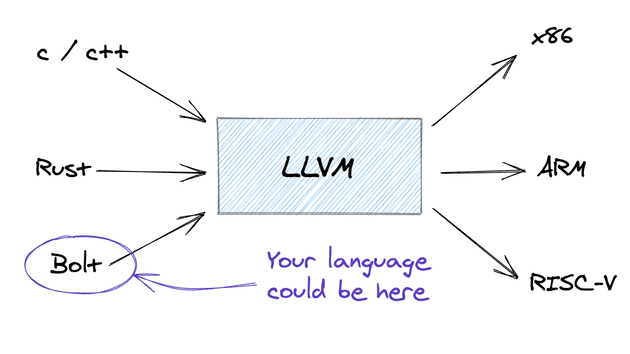
\includegraphics[width=\linewidth]{08_files/llvm.png}

%\hypertarget{series-creating-the-bolt-compiler}{%
%\section{Series: Creating the Bolt
%Compiler}\label{series-creating-the-bolt-compiler}}
%
%\begin{itemize}
%\item
%  { Part 1:
%  }\href{https://mukulrathi.com/create-your-own-programming-language/intro-to-compiler/}{How
%  I wrote my own "proper" programming language}
%\item
%  { Part 2:
%  }\href{https://mukulrathi.com/create-your-own-programming-language/compiler-engineering-structure/}{So
%  how do you structure a compiler project?}
%\item
%  { Part 3:
%  }\href{https://mukulrathi.com/create-your-own-programming-language/parsing-ocamllex-menhir/}{Writing
%  a Lexer and Parser using OCamllex and Menhir}
%\item
%  { Part 4:
%  }\href{https://mukulrathi.com/create-your-own-programming-language/intro-to-type-checking/}{An
%  accessible introduction to type theory and implementing a
%  type-checker}
%\item
%  { Part 5:
%  }\href{https://mukulrathi.com/create-your-own-programming-language/data-race-dataflow-analysis/}{A
%  tutorial on liveness and alias dataflow analysis}
%\item
%  { Part 6:
%  }\href{https://mukulrathi.com/create-your-own-programming-language/lower-language-constructs-to-llvm/}{Desugaring
%  - taking our high-level language and simplifying it!}
%\item
%  { Part 7:
%  }\href{https://mukulrathi.com/create-your-own-programming-language/protobuf-ocaml-cpp-tutorial/}{A
%  Protobuf tutorial for OCaml and C++}
%\item
%  \textbf{Part 8: A Complete Guide to LLVM for Programming Language
%  Creators}
%\item
%  { Part 9:
%  }\href{https://mukulrathi.com/create-your-own-programming-language/concurrency-runtime-language-tutorial/}{Implementing
%  Concurrency and our Runtime Library}
%\item
%  { Part 10:
%  }\href{https://mukulrathi.com/create-your-own-programming-language/generics-parametric-polymorphism/}{Generics
%  - adding polymorphism to Bolt}
%\item
%  { Part 11:
%  }\href{https://mukulrathi.com/create-your-own-programming-language/inheritance-method-overriding-vtable/}{Adding
%  Inheritance and Method Overriding to Our Language}
%\end{itemize}
%
%\begin{center}\rule{0.5\linewidth}{0.5pt}\end{center}

\textbf{Update}: this post has now taken off on
\href{https://news.ycombinator.com/item?id=25539797}{Hacker News} and
\href{https://www.reddit.com/r/programming/comments/kjjijf/a_complete_guide_to_llvm_for_programming_language/}{Reddit}.
Thank you all!

\hypertarget{whos-this-tutorial-for}{%
\section{\texorpdfstring{\protect\hyperlink{whos-this-tutorial-for}{}Who's
this tutorial
for?}{Who's this tutorial for?}}\label{whos-this-tutorial-for}}

This series of compiler tutorials is for people who don't just want to
create a \emph{toy} language. You want objects. You want polymorphism.
You want concurrency. You want garbage collection. Wait you don't want
GC? Okay, no worries, we won't do that :P

If you've just joined the series at this stage, here's a quick recap.
We're designing a Java-esque concurrent object-oriented programming
language \emph{Bolt}. We've gone through the compiler frontend, where
we've done the parsing, type-checking and dataflow analysis. We've
\href{https://mukulrathi.com/create-your-own-programming-language/lower-language-constructs-to-llvm/}{desugared
our language to get it ready for LLVM} - the main takeaway is that
objects have been desugared to structs, and their methods desugared to
functions.

Learn about LLVM and you'll be the envy of your friends. Rust uses LLVM
for its backend, so it must be cool. You'll beat them on all those
performance benchmarks, without having to hand-optimise your code or
write machine assembly code. Shhhh, I won't tell them.

\hypertarget{just-give-me-the-code}{%
\section{\texorpdfstring{\protect\hyperlink{just-give-me-the-code}{}Just
give me the
code!}{Just give me the code!}}\label{just-give-me-the-code}}

All the code can be found in the
\href{https://github.com/mukul-rathi/bolt}{Bolt compiler repository}.

The C++ class definitions for our desugared representation (we call this
\emph{Bolt IR}) can be found in
\href{https://github.com/mukul-rathi/bolt/tree/master/src/llvm-backend/deserialise_ir}{deserialise\_ir}
folder. The code for this post (the LLVM IR generation) can be found in
the
\href{https://github.com/mukul-rathi/bolt/tree/master/src/llvm-backend/llvm_ir_codegen}{llvm\_ir\_codegen}
folder. The repo uses the Visitor design pattern and ample use of
\texttt{std::unique\_ptr} to make memory management easier.

To cut through the boilerplate, to find out how to generate LLVM IR for
a particular language expression, search for the
\texttt{IRCodegenVisitor::codegen} method that takes in the
corresponding \texttt{ExprIR} object. e.g. for if-else statements:

%Copy

\begin{lstlisting}[language=C++]
Value *IRCodegenVisitor::codegen(const ExprIfElseIR &expr) {
      ...
 // this is the LLVM IR generation
}
\end{lstlisting}

\hypertarget{understanding-llvm-ir}{%
\section{\texorpdfstring{\protect\hyperlink{understanding-llvm-ir}{}Understanding
LLVM IR}{Understanding LLVM IR}}\label{understanding-llvm-ir}}

LLVM sits in the \textbf{middle-end} of our compiler, \emph{after} we've
desugared our language features, but \emph{before} the backends that
target specific machine architectures (x86, ARM etc.)

LLVM's IR is pretty low-level, it can't contain language features
present in some languages but not others (e.g. classes are present in
C++ but not C). If you've come across instruction sets before, LLVM IR
is a
\href{https://en.wikipedia.org/wiki/Reduced_instruction_set_computer\#:~:text=A\%20reduced\%20instruction\%20set\%20computer,instruction\%20set\%20computer\%20(CISC).}{RISC}
instruction set.

The upshot of it is that LLVM IR looks like a more \emph{readable} form
of assembly. As LLVM IR is \textbf{machine independent}, we don't need
to worry about the number of registers, size of datatypes, calling
conventions or other machine-specific details.

So instead of a fixed number of physical registers, in LLVM IR we have
an unlimited set of \emph{virtual} registers (labelled \texttt{\%0},
\texttt{\%1}, \texttt{\%2}, \texttt{\%3}\ldots{} we can write and read
from. It's the backend's job to map from virtual to physical registers.

And rather than allocating specific sizes of datatypes, we retain
\textbf{types} in LLVM IR. Again, the backend will take this type
information and map it to the size of the datatype. LLVM has types for
different sizes of \texttt{int}s and floats, e.g. \texttt{int32},
\texttt{int8}, \texttt{int1} etc. It also has derived types: like
\textbf{pointer} types, \textbf{array} types, \textbf{struct} types,
\textbf{function} types. To find out more, check out the
\href{https://llvm.org/doxygen/classllvm_1_1Type.html}{Type}
documentation.

Now, built into LLVM are a set of optimisations we can run over the LLVM
IR e.g.
\href{https://en.wikipedia.org/wiki/Dead_code_elimination}{dead-code
elimination},
\href{https://en.wikipedia.org/wiki/Inline_expansion}{function
inlining},
\href{https://cran.r-project.org/web/packages/rco/vignettes/opt-common-subexpr.html}{common
subexpression elimination} etc. The details of these algorithms are
irrelevant: LLVM implements them for us.

Our side of the bargain is that we write LLVM IR in
\href{https://en.wikipedia.org/wiki/Static_single_assignment_form}{Static
Single Assignment (SSA) form}, as SSA form makes life easier for
optimisation writers. SSA form sounds fancy, but it just means we define
variables before use and assign to variables \textbf{only once}. In SSA
form, we cannot reassign to a variable, e.g. \texttt{x\ =\ x+1}; instead
we assign to a fresh variable each time (\texttt{x2\ =\ x1\ +\ 1}).

So in short: LLVM IR looks like assembly with \textbf{types}, minus the
messy machine-specific details. LLVM IR must be in SSA form, which makes
it easier to optimise. Let's look at an example!

\hypertarget{an-example-factorial}{%
\subsection{\texorpdfstring{\protect\hyperlink{an-example-factorial}{}An
example: Factorial}{An example: Factorial}}\label{an-example-factorial}}

Let's look at a simple factorial function in our language Bolt:



%Copy

\begin{lstlisting}[caption={{factorial.bolt}}]
function int factorial(int n){
  if (n==0) {    1  }
  else{    n * factorial(n - 1)  }
}
\end{lstlisting}

The corresponding LLVM IR is as follows:



%Copy

\begin{lstlisting}[caption={{factorial.ll}},language=llvm]
define i32 @factorial(i32) {
entry:
  %eq = icmp eq i32 %0, 0   // n == 0
  br i1 %eq, label %then, label %else

then:                                             ; preds = %entry
  br label %ifcont

else:                                             ; preds = %entry
  %sub = sub i32 %0, 1   // n - 1
  %2 = call i32 @factorial(i32 %sub) // factorial(n-1)
  %mult = mul i32 %0, %2  // n * factorial(n-1)
  br label %ifcont

ifcont:                                           ; preds = %else, %then
  %iftmp = phi i32 [ 1, %then ], [ %mult, %else ]
  ret i32 %iftmp
}
\end{lstlisting}

Note the \texttt{.ll} extension is for \textbf{human-readable} LLVM IR
output. There's also \texttt{.bc} for bit-code, a more compact machine
representation of LLVM IR.

We can walk through this IR in 4 levels of detail:

\hypertarget{at-the-instruction-level}{%
\paragraph{\texorpdfstring{\protect\hyperlink{at-the-instruction-level}{}At
the Instruction
Level:}{At the Instruction Level:}}\label{at-the-instruction-level}}

Notice how LLVM IR contains assembly instructions like \texttt{br} and
\texttt{icmp}, but abstracts the machine-specific messy details of
function calling conventions with a single \texttt{call} instruction.

{
\href{https://mukulrathi.com/static/f987ee45552570ad7aa513f6d3fc19a7/565cc/factorial-instructions.png}{{}
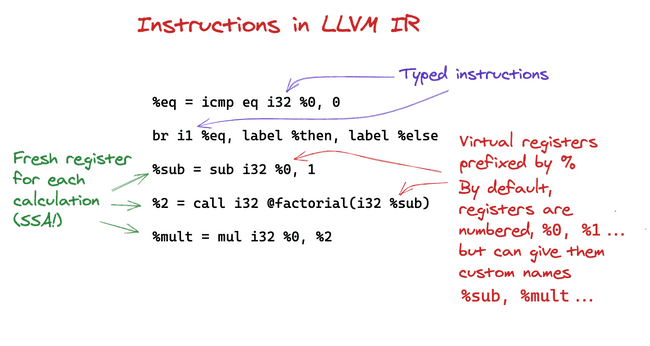
\includegraphics[width=\linewidth]{08_files/factorial-instructions.png}} }

\hypertarget{at-the-control-flow-graph-level}{%
\paragraph{\texorpdfstring{\protect\hyperlink{at-the-control-flow-graph-level}{}At
the Control Flow Graph
Level:}{At the Control Flow Graph Level:}}\label{at-the-control-flow-graph-level}}

If we take a step back, you can see the IR defines the \textbf{control
flow graph} of the program. IR instructions are grouped into labeled
\textbf{basic blocks}, and the \texttt{preds} labels for each block
represent incoming edges to that block. e.g. the \texttt{ifcont} basic
block has predecessors \texttt{then} and \texttt{else}:

At this point, I'm going to assume you have come across Control Flow
Graphs and basic blocks. We introduced Control Flow Graphs in a previous
post in the series, where we used them to perform different dataflow
analyses on the program. I'd recommend you go and check the
\href{http://mukulrathi.co.uk/create-your-own-programming-language/data-race-dataflow-analysis/\#control-flow-graph}{CFG
section of that dataflow analysis post} now. I'll wait here :)

{
\href{https://mukulrathi.com/static/6a6edf6d916150ea4de92c0fc1a68e1a/11864/factorial-cfg.png}{{}
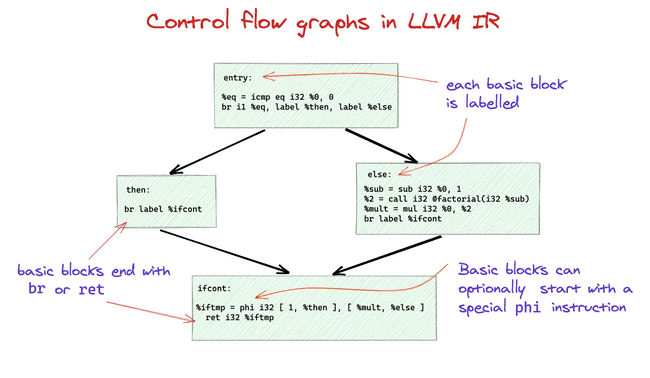
\includegraphics[width=\linewidth]{08_files/factorial-cfg.png}} }

The \texttt{phi} instruction represents \textbf{conditional assignment}:
assigning different values depending on which preceding basic block
we've just come from. It is of the form
\texttt{phi\ type\ {[}val1,\ predecessor1{]},\ {[}val2,\ predecessor2{]},\ ...}
In the example above, we set \texttt{\%iftmp} to 1 if we've come from
the \texttt{then} block, and \texttt{\%mult} if we've come from the
\texttt{else} block. Phi nodes must be at the \textbf{start} of a block,
and include one entry for each predecessor.

\hypertarget{at-the-function-level}{%
\paragraph{\texorpdfstring{\protect\hyperlink{at-the-function-level}{}At
the Function
Level:}{At the Function Level:}}\label{at-the-function-level}}

Taking another step back, the overall structure of a function in LLVM IR
is as follows:

{
\href{https://mukulrathi.com/static/c80bbba94459a0ac84429c53299823b2/b2b2c/factorial-fn.png}{{}
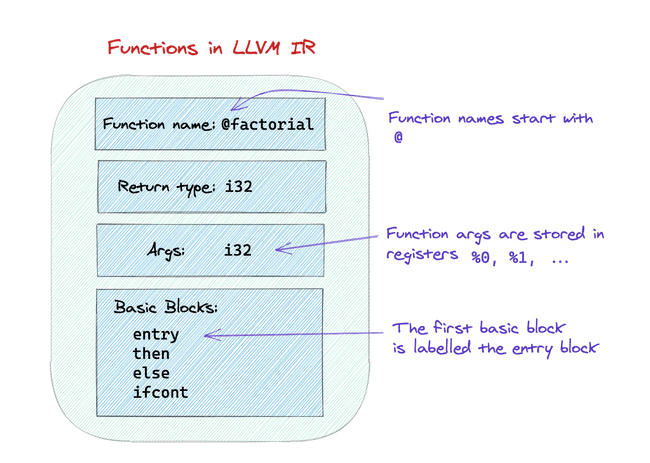
\includegraphics[width=\linewidth]{08_files/factorial-fn.png}} }

\hypertarget{at-the-module-level}{%
\paragraph{\texorpdfstring{\protect\hyperlink{at-the-module-level}{}At
the Module Level:}{At the Module Level:}}\label{at-the-module-level}}

An LLVM \textbf{module} contains all the information associated with a
program file. (For multi-file programs, we'd link together their
corresponding modules.)

{
\href{https://mukulrathi.com/static/e21edb9623d8fb7bc23f57db23b93cf8/cad61/module.png}{{}
\includegraphics[width=\linewidth]{08_files/module.png}} }

Our \texttt{factorial} function is just one function definition in our
module. If we want to execute the program, e.g. to compute
\texttt{factorial(10)} we need to define a \texttt{main} function, which
will be the entrypoint for our program's execution. The \texttt{main}
function's signature is a hangover from C (we return 0 to indicate
successful execution):



%Copy

\begin{lstlisting}[caption={{example\_program.c}},language=C]
// a C main function
int main(){
  factorial(10);
  return 0;
}
\end{lstlisting}

We specify that we want to compile for an Intel Macbook Pro in the
module target info:



%Copy

\begin{lstlisting}[caption={{example\_module.ll}},language=llvm]
source_filename = "Module"
target triple = "x86_64-apple-darwin18.7.0"
...
define i32 @factorial(i32) {
  ...
}
define i32 @main() {
entry:
  %0 = call i32 @factorial(i32 10)
  ret i32 0
}
\end{lstlisting}

\hypertarget{the-llvm-api-key-concepts}{%
\section{\texorpdfstring{\protect\hyperlink{the-llvm-api-key-concepts}{}The
LLVM API: Key
Concepts}{The LLVM API: Key Concepts}}\label{the-llvm-api-key-concepts}}

Now we've got the basics of LLVM IR down, let's introduce the LLVM API.
We'll go through the key concepts, then introduce more of the API as we
explore LLVM IR further.

LLVM defines a whole host of classes that map to the concepts we've
talked about.

\begin{itemize}
\tightlist
\item
  \texttt{Value}
\item
  \texttt{Module}
\item
  \texttt{Type}
\item
  \texttt{Function}
\item
  \texttt{BasicBlock}
\item
  \texttt{BranchInst} \ldots{}
\end{itemize}

These are all in the namespace \texttt{llvm}. In the Bolt repo, I chose
to make this namespacing explicit by referring to them as
\texttt{llvm::Value}, \texttt{llvm::Module} etc.)

Most of the LLVM API is quite mechanical. Now you've seen the diagrams
that define modules, functions and basic blocks, the relationship
between their corresponding classes in the API falls out nicely. You can
query a \texttt{Module} object to get a list of its \texttt{Function}
objects, and query a \texttt{Function} to get the list of its
\texttt{BasicBlock}s, and the other way round: you can query a
\texttt{BasicBlock} to get its parent \texttt{Function} object.

\texttt{Value} is the base class for any value computed by the program.
This could be a function (\texttt{Function} subclasses \texttt{Value}),
a basic block (\texttt{BasicBlock} also subclasses \texttt{Value}), an
instruction, or the result of an intermediate computation.

Each of the expression \texttt{codegen} methods returns a
\texttt{Value\ *}: the result of executing that expression. You can
think of these \texttt{codegen} methods as generating the IR for that
expression and the \texttt{Value\ *} representing the virtual register
containing the expression's result.

%{
%\href{https://github.com/mukul-rathi/bolt/blob/master/src/llvm-backend/llvm_ir_codegen/ir_codegen_visitor.h\#L64-L84}{ir\_codegen\_visitor.h}}
%
%Copy

\begin{lstlisting}[caption={ir\_codegen\_visitor.h},language=C++]
virtual Value *codegen(const ExprIntegerIR &expr) override;
virtual Value *codegen(const ExprBooleanIR &expr) override;
virtual Value *codegen(const ExprIdentifierIR &expr) override;
virtual Value *codegen(const ExprConstructorIR &expr) override;
virtual Value *codegen(const ExprLetIR &expr) override;
virtual Value *codegen(const ExprAssignIR &expr) override;
\end{lstlisting}

How do we generate the IR for these expressions? We create a
\textbf{unique} \texttt{Context} object to tie our whole code generation
together. We use this \texttt{Context} to get access to core LLVM data
structures e.g LLVM modules and \texttt{IRBuilder} objects.

We'll use the context to create just one module, which we'll
imaginatively name \texttt{"Module"}.

%{
%\href{https://github.com/mukul-rathi/bolt/blob/master/src/llvm-backend/llvm_ir_codegen/ir_codegen_visitor.cc\#L17-L19}{ir\_codegen\_visitor.cc}}
%
%Copy

\begin{lstlisting}[language=C++,caption={ir\_codegen\_visitor.cc}]
context = make_unique<LLVMContext>();
builder = std::unique_ptr<IRBuilder<>>(new IRBuilder<>(*context));
module = make_unique<Module>("Module", *context);
\end{lstlisting}

\hypertarget{irbuilder}{%
\subsection{\texorpdfstring{\protect\hyperlink{irbuilder}{}IRBuilder}{IRBuilder}}\label{irbuilder}}

We use the \texttt{IRBuilder} object to incrementally build up our IR.
It is intuitively the equivalent of a file pointer when reading/writing
a file - it carries around \emph{implicit} state, e.g. the last
instruction added, the basic block of that instruction etc. Like moving
around a file pointer, you can set the \texttt{builder} object to insert
instructions at the end of a particular Basic Block with the
\texttt{SetInsertPoint(BasicBlock\ *TheBB)} method. Likewise you can get
the current basic block with \texttt{GetInsertBlock()}.

The builder object has \texttt{Create\_\_\_()} methods for each of the
IR instructions. e.g. \texttt{CreateLoad} for a \texttt{load}
instruction , \texttt{CreateSub}, \texttt{CreateFSub} for integer and
floating point \texttt{sub} instructions respectively etc. Some
\texttt{Create\_\_()} instructions take an optional \texttt{Twine}
argument: this is used to give the result's register a custom name. e.g.
\texttt{iftmp} is the twine for the following instruction:

\texttt{\%iftmp\ =\ phi\ i32\ {[}\ 1,\ \%then\ {]},\ {[}\ \%mult,\ \%else{]}}

Use \href{https://llvm.org/doxygen/classllvm_1_1IRBuilderBase.html}{the
IRBuilder docs} to find the method corresponding to your instruction.

\hypertarget{types-and-constants}{%
\subsection{\texorpdfstring{\protect\hyperlink{types-and-constants}{}Types
and Constants}{Types and Constants}}\label{types-and-constants}}

We don't directly construct these, instead we \texttt{get\_\_()} them
from their corresponding classes. (LLVM keeps track of how a unique
instance of each type / constant class is used).

For example, we \texttt{getSigned} to get a constant signed integer of a
particular type and value, and \texttt{getInt32Ty} to get the
\texttt{int32} type.

%{
%\href{https://github.com/mukul-rathi/bolt/blob/master/src/llvm-backend/llvm_ir_codegen/expr_codegen.cc\#L39-L42}{expr\_codegen.cc}}
%
%Copy

\begin{lstlisting}[language=C++,caption={expr\_codegen.cc}]
Value *IRCodegenVisitor::codegen(const ExprIntegerIR &expr){
 return ConstantInt::getSigned((Type::getInt32Ty(*context)),
                                      expr.val);
};
\end{lstlisting}

Function types are similar: we can use \texttt{FunctionType::get}.
Function types consist of the return type, an array of the types of the
params and whether the function is
\href{https://en.wikipedia.org/wiki/Variadic_function}{variadic}:

%{
%\href{https://github.com/mukul-rathi/bolt/blob/master/src/llvm-backend/llvm_ir_codegen/function_codegen.cc\#L18-L19}{function\_codegen.cc}}
%
%Copy

\begin{lstlisting}[language=C++,caption={{function\_codegen.cc}}]
FunctionType::get(returnType, paramTypes, false /* doesn't have variadic args */);
\end{lstlisting}

\hypertarget{type-declarations}{%
\subsection{\texorpdfstring{\protect\hyperlink{type-declarations}{}Type
declarations}{Type declarations}}\label{type-declarations}}

We can declare our own custom struct types.

e.g. a Tree with a \texttt{int} value, and pointers to left and right
subtrees:

%Copy

\begin{lstlisting}[language=llvm]
%Tree = type {i32, Tree*, Tree* }
\end{lstlisting}

Defining a custom struct type is a two-stage process.

First we create the type with that name. This adds it to the module's
\textbf{symbol table}. This type is \textbf{opaque}: we can now
reference in other type declarations e.g. function types, or other
struct types, but we can't create structs of that type (as we don't know
what's in it).

%Copy

\begin{lstlisting}[language=C++]
StructType *treeType = StructType::create(*context, StringRef("Tree"));
\end{lstlisting}

LLVM boxes up strings and arrays using \texttt{StringRef} and
\texttt{ArrayRef}. You can directly pass in a string where the docs
require a StringRef, but I choose to make this \texttt{StringRef}
explicit above.

The second step is to specify an array of types that go in the struct
body. Note since we've defined the opaque \texttt{Tree} type, we can get
a \texttt{Tree\ *} type using the \texttt{Tree} type's
\texttt{getPointerTo()} method.

Copy

\begin{verbatim}
treeType->setBody(ArrayRef<Type *>({Type::getInt32Ty(*context);, treeType->getPointerTo(), treeType->getPointerTo()}));
\end{verbatim}

So if you have custom struct types referring to other custom struct
types in their bodies, the best approach is to declare all of the opaque
custom struct types, \emph{then} fill in each of the structs' bodies.

%{
%\href{https://github.com/mukul-rathi/bolt/blob/master/src/llvm-backend/llvm_ir_codegen/class_codegen.cc\#L10-L39}{class\_codegen.cc}}
%
%Copy

\begin{lstlisting}[language=C++,caption={class\_codegen.cc}]
void IRCodegenVisitor::codegenClasses(
    const std::vector<std::unique_ptr<ClassIR>> &classes) {
  // create (opaque) struct types for each of the classes
  for (auto &currClass : classes) {
    StructType::create(*context, StringRef(currClass->className));
  }
  // fill in struct bodies
  for (auto &currClass : classes) {
    std::vector<Type *> bodyTypes;
    for (auto &field : currClass->fields) {
          // add field type
          bodyTypes.push_back(field->codegen(*this));
    }
    // get opaque class struct type from module symbol table
    StructType *classType =
        module->getTypeByName(StringRef(currClass->className));
    classType->setBody(ArrayRef<Type *>(bodyTypes));
  }
\end{lstlisting}

\subsubsection{Functions}

Functions operate in a similar two step process:

\begin{enumerate}
\tightlist
\item
  Define the function prototypes
\item
  Fill in their function bodies (skip this if you're linking in an
  external function!)
\end{enumerate}

The function prototype consists of the function name, the function type,
the ``linkage'' information and the module whose symbol table we want to
add the function to. We choose External linkage - this means the
function prototype is viewable externally. This means that we can link
in an external function definition (e.g. if using a library function),
or expose our function definition in another module. You can see the
full
\href{https://llvm.org/doxygen/classllvm_1_1GlobalValue.html\#aedfa75f0c85c4aa85b257f066fbea57c}{enum
of linkage options here}.

%{
%\href{https://github.com/mukul-rathi/bolt/blob/master/src/llvm-backend/llvm_ir_codegen/function_codegen.cc\#L27-L28}{function\_codegen.cc}}
%
%Copy

\begin{lstlisting}[caption={function\_codegen.cc},language=C++]
Function::Create(functionType, Function::ExternalLinkage,
                           function->functionName, module.get());
\end{lstlisting}

To generate the function definition we just need to use the API to
construct the control flow graph we discussed in our \texttt{factorial}
example:

%{
%\href{https://github.com/mukul-rathi/bolt/blob/master/src/llvm-backend/llvm_ir_codegen/function_codegen.cc\#L32-L37}{function\_codegen.cc}}
%
%Copy

\begin{lstlisting}[language=C++,caption={function\_codegen.cc}]
void IRCodegenVisitor::codegenFunctionDefn(const FunctionIR &function) {
  // look up function in module symbol definition
  Function *llvmFun =
      module->getFunction(function.functionName);
  BasicBlock *entryBasicBlock =
      BasicBlock::Create(*context, "entry", llvmFun);
  builder->SetInsertPoint(entryBasicBlock);
  ...
\end{lstlisting}

The official Kaleidoscope tutorial has an excellent explanation of
\href{https://llvm.org/docs/tutorial/MyFirstLanguageFrontend/LangImpl05.html\#code-generation-for-if-then-else}{how
to construct a control flow graph for an if-else statement}.

\hypertarget{more-llvm-ir-concepts}{%
\section{\texorpdfstring{\protect\hyperlink{more-llvm-ir-concepts}{}More
LLVM IR Concepts}{More LLVM IR Concepts}}\label{more-llvm-ir-concepts}}

Now we've covered the basics of LLVM IR and the API, we're going to look
at some more LLVM IR concepts and introduce the corresponding API
function calls alongside them.

\hypertarget{stack-allocation}{%
\section{\texorpdfstring{\protect\hyperlink{stack-allocation}{}Stack
allocation}{Stack allocation}}\label{stack-allocation}}

There are two ways we can store values in local variables in LLVM IR.
We've seen the first: \textbf{assignment to virtual registers}. The
second is \textbf{dynamic memory allocation} to the stack using the
\texttt{alloca} instruction. Whilst we can store ints, floats and
pointers to either the stack or virtual registers, \textbf{aggregate}
datatypes, like structs and arrays, don't fit in registers so have to be
stored on the stack.

Yes, you read that right. Unlike most programming language memory
models, where we use the heap for dynamic memory allocation, in LLVM we
just have a stack.

Heaps are not provided by LLVM - they are a \emph{library} feature. For
single-threaded applications, stack allocation is sufficient. We'll talk
about the need for a global heap in multi-threaded programs in the next
post (where we extend Bolt to support concurrency).

We've seen struct types e.g. \texttt{\{i32,\ i1,\ i32\}}. Array types
are of the form \texttt{{[}num\_elems\ x\ elem\_type{]}}. Note
\texttt{num\_elems} is a constant - you need to provide this when
generating the IR, not at runtime. So \texttt{{[}3\ x\ int32{]}} is
valid but \texttt{{[}n\ x\ int32{]}} is not.

We give \texttt{alloca} a type and it allocates a block of memory on the
stack and returns a \emph{pointer} to it, which we can store in a
register. We can use this pointer to load and store values from/onto the
stack.

For example, storing a 32-bit int on the stack:

%Copy

\begin{lstlisting}[language=llvm]
%p = alloca i32 // store i32* pointer in %p
 store i32 1, i32* %p
 %1 = load i32, i32* %p
\end{lstlisting}

The corresponding builder instructions are\ldots{} you guessed it
\texttt{CreateAlloca}, \texttt{CreateLoad}, \texttt{CreateStore}.
\texttt{CreateAlloca} returns a special subclass of \texttt{Value\ *}:
an \texttt{AllocaInst\ *}:

%Copy

\begin{lstlisting}[language=C++]
AllocaInst *ptr = builder->CreateAlloca(Type::getInt32Ty(*context),
                                         /* Twine */ "p");
// AllocaInst has additional methods e.g. to query type
ptr->getAllocatedType(); // returns i32
builder->CreateLoad(ptr);
builder->CreateStore(someVal, ptr);
\end{lstlisting}

\hypertarget{global-variables}{%
\section{\texorpdfstring{\protect\hyperlink{global-variables}{}Global
variables}{Global variables}}\label{global-variables}}

Just as we \texttt{alloca} local variables on a stack, we can create
global variables and \texttt{load} from them and \texttt{store} to them.

Global variables are declared at the start of a module, and are part of
the module symbol table.

{
\href{https://mukulrathi.com/static/c681b04ecad4a94c9d9144a337051ac9/74dae/global-variables.png}{{}
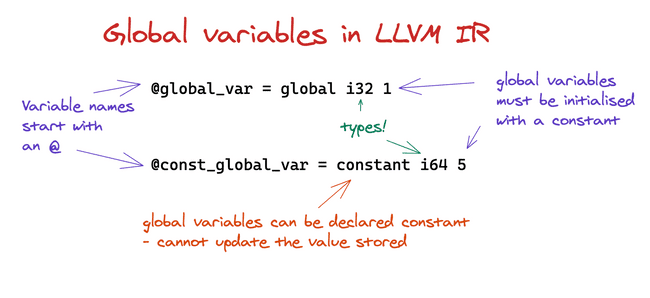
\includegraphics[width=\linewidth]{08_files/global-variables.png}} }

We can use the \texttt{module} object to create named global variables,
and to query them.

%Copy

\begin{verbatim}
module->getOrInsertGlobal(globalVarName, globalVarType);
...
GlobalVariable *globalVar = module->getNamedGlobal(globalVarName);
\end{verbatim}

Global variables \textbf{must} be initialised with a constant value (not
a variable):

%Copy

\begin{verbatim}
globalVar->setInitializer(initValue);
\end{verbatim}

Alternatively we can do this in one command using the
\texttt{GlobalVariable} constructor:

%Copy

\begin{lstlisting}[language=C++]
GlobalVariable *globalVar = new GlobalVariable(module, globalVarType, /*isConstant*/ false,              GlobalValue::ExternalLinkage, initValue, globalVarName)
\end{lstlisting}

As before we can \texttt{load} and \texttt{store}:

%Copy

\begin{verbatim}
builder->CreateLoad(globalVar);
builder->CreateStore(someVal, globalVar); // not for consts!
\end{verbatim}

\hypertarget{geps}{%
\section{\texorpdfstring{\protect\hyperlink{geps}{}GEPs}{GEPs}}\label{geps}}

We get a \textbf{base pointer} to the aggregate type (array / struct) on
the stack or in global memory, but what if we want a pointer to a
\textbf{specific element}? We'd need to find the \textbf{pointer offset}
of that element within the aggregate, and then add this to the base
pointer to get the address of that element. Calculating the pointer
offset is machine-specific e.g. depends on the size of the datatypes,
the struct padding etc.

The Get Element Pointer (GEP) instruction is an instruction to apply the
pointer offset to the base pointer and return the resultant
\textbf{pointer}.

Consider two arrays starting at \texttt{p}. Following C convention, we
can represent a pointer to that array as \texttt{char*} or
\texttt{int*}.

{
\href{https://mukulrathi.com/static/72077af5568512fb3538183382b672b0/a9577/pointer-offset.png}{{}
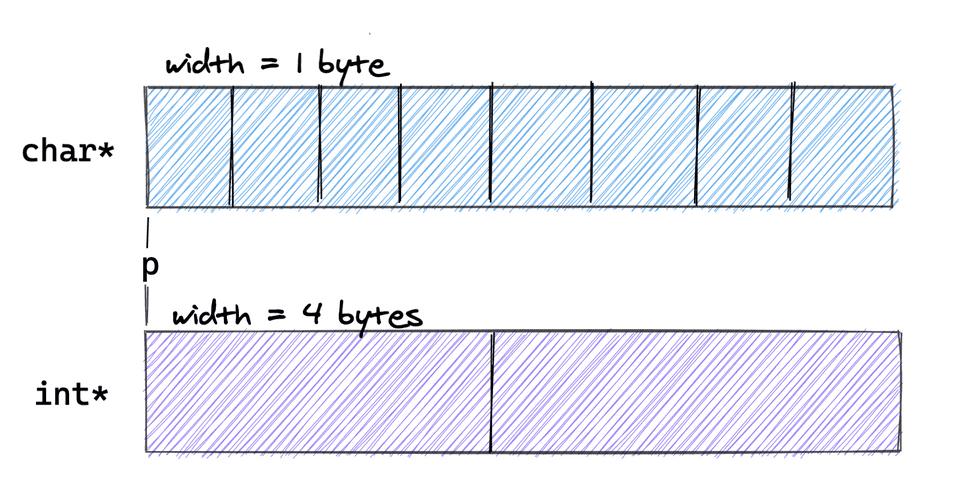
\includegraphics[width=\linewidth]{08_files/pointer-offset.png}} }

Below we show the GEP instruction to calculate the pointer \texttt{p+1}
in each of the arrays:

%Copy

\begin{lstlisting}[language=llvm]
// char = 8 bit integer = i8
%idx1 = getelementptr i8, i8* %p, i64 1 // p + 1 for char*
%idx2 = getelementptr i32, i32* %p, i64 1 // p + 1 for int*
\end{lstlisting}

This GEP instruction is a bit of a mouthful so here's a breakdown:

{
\href{https://mukulrathi.com/static/c54f577c6586b64d172044af4f8aacd1/79166/gep-int.png}{{}
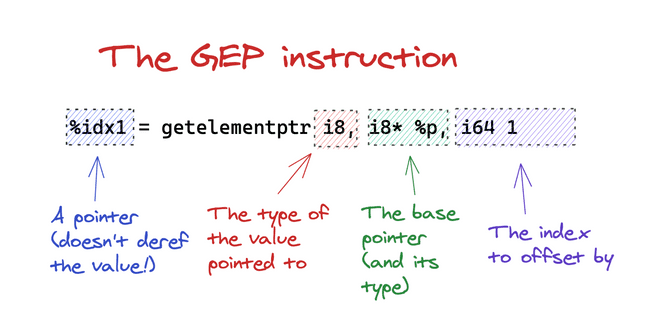
\includegraphics[width=\linewidth]{08_files/gep-int.png}} }

This \texttt{i64\ 1} index adds \textbf{multiples} of the base type to
the base pointer. \texttt{p+1} for \texttt{i8} would add 1 byte, whereas
as \texttt{p+1} for \texttt{i32} would add 4 bytes to \texttt{p}. If the
index was \texttt{i64\ 0} we'd return \texttt{p} itself.

The LLVM API instruction for creating a GEP is\ldots{}
\texttt{CreateGEP}.

%Copy

\begin{verbatim}
Value *ptr = builder->CreateGEP(baseType, basePtr, arrayofIndices);
\end{verbatim}

Wait? \emph{Array} of indices? Yes, the GEP instruction can have
multiple indices passed to it. We've looked at a simple example where we
only needed one index.

Before we look at the case where we pass multiple indices, I want to
reiterate the purpose of this first index:

\emph{\textbf{A pointer of type \texttt{Foo\ *} can represent in C the
base pointer of an array of type \texttt{Foo}. The first index adds
multiples of this base type Foo to traverse this array.}}

\hypertarget{geps-with-structs}{%
\subsection{\texorpdfstring{\protect\hyperlink{geps-with-structs}{}GEPS
with Structs}{GEPS with Structs}}\label{geps-with-structs}}

Okay, now let's look at structs. So take a struct of type \texttt{Foo}:

%Copy

\begin{lstlisting}[language=llvm]
%Foo = type { i32, [4 x i32], i32}
\end{lstlisting}

We want to index \textbf{specific} fields in the struct. The natural way
would be to label them field \texttt{0}, \texttt{1} and \texttt{2}. We
can access field \texttt{2} by passing this into the GEP instruction as
\textbf{another index}.

%Copy

\begin{lstlisting}[language=llvm]
%ThirdFieldPtr = getelementptr  %Foo, %Foo* %ptr, i64 0, i64 2
\end{lstlisting}

The returned pointer is then calculated as:
\texttt{ptr\ +\ 0\ *\ (size\ of\ Foo)\ +\ offset\ 2\ *\ (fields\ of\ Foo)}.

For structs, you'll likely always pass the first index as \texttt{0}.
The biggest confusion with GEPs is that this \texttt{0} can seem
redundant, as we want the field \texttt{2}, so why are we passing a
\texttt{0} index first? Hopefully you can see from the first example why
we need that \texttt{0}. Think of it as passing to GEP the base pointer
of an implicit \texttt{Foo} array of size 1.

To avoid the confusion, LLVM has a special \texttt{CreateStructGEP}
instruction that asks only for field index (this is the
\texttt{CreateGEP} instruction with a \texttt{0} added for you):

%Copy

\begin{verbatim}
Value *thirdFieldPtr = builder->CreateStructGEP(baseStructType, basePtr, fieldIndex);
\end{verbatim}

The more nested our aggregate structure, the more indices we can
provide. E.g. for element index \texttt{2} of Foo's second field (the 4
element int array):

%Copy

\begin{lstlisting}[language=llvm]
getelementptr  %Foo, %Foo* %ptr, i64 0, i64 1, i64 2
\end{lstlisting}

The pointer returned is:
\texttt{ptr\ +\ 0\ *\ (size\ of\ Foo)\ +\ offset\ 1\ *\ (field\ of\ Foo)\ +\ offset\ 2\ *\ (elems\ of\ array)}.
(In terms of the corresponding API, we'd use \texttt{CreateGEP} and pass
the array \texttt{\{0,1,2\}}.)
%\href{https://youtu.be/m8G_S5LwlTo?t=1753}
{A Good talk that explains GEP
well:\url{https://youtu.be/m8G_S5LwlTo?t=1753}}

\hypertarget{mem2reg}{%
\section{\texorpdfstring{\protect\hyperlink{mem2reg}{}mem2reg}{mem2reg}}\label{mem2reg}}

If you remember, LLVM IR must be written in SSA form. But what happens
if the Bolt source program we're trying to map to LLVM IR is not in SSA
form? For example, if we're reassigning \texttt{x}:

%{reassign\_var.bolt}

%Copy

\begin{verbatim}
let x = 1
x = x + 1
\end{verbatim}

One option would be for us to rewrite the program in SSA form in an
earlier compiler stage. Every time we reassign a variable, we'd have to
create a fresh variable. We'd also have to introduce \texttt{phi} nodes
for conditional statements. For our example, this is straightforward,
but in general this extra rewrite is a pain we would rather not deal
with.

%{assign\_fresh\_vars.bolt}

%Copy

\begin{verbatim}
// Valid SSA: assign fresh variables
let x1 = 1
    x2 = x1 + 1
\end{verbatim}

We can use \textbf{pointers} to avoid assigning fresh variables. Note
here we \textbf{aren't reassigning} the pointer \texttt{x}, just
updating \textbf{the value it pointed to}. So this is valid SSA.

%Copy

\begin{verbatim}
// valid SSA: use a pointer and update the value it points to
let x = &1;
   *x = *x + 1
\end{verbatim}

This switch to pointers is a much easier transformation than variable
renaming. It also has a really nice LLVM IR equivalent: allocating
\emph{stack memory} (and manipulating the pointers to the stack) instead
of reading from \emph{registers}.

So whenever we declare a local variable, we use \texttt{alloca} to get a
pointer to freshly allocated stack space. We use the \texttt{load} and
\texttt{store} instructions to read and update the value pointed to by
the pointer:

%{reassign\_var.ll}
%
%Copy

\begin{lstlisting}[language=llvm]
%x = alloca i32
store i32 1, i32* %x

%1 = load i32, i32* %x
%2 = add i32 %1, 1
store i32 %2, i32* %x
\end{lstlisting}

Let's revisit the LLVM IR if we were to rewrite the Bolt program to use
fresh variables. It's only \emph{2} instructions, compared to the
\emph{5} instructions needed if using the stack. Moreover, we avoid the
expensive \texttt{load} and \texttt{store} memory access instructions.

%{assign\_fresh\_vars.ll}
%
%Copy

\begin{lstlisting}[language=llvm]
%x1 = 1
%x2 = add i32 %x1, 1   // let x2 = x1 + 1
\end{lstlisting}

So while we've made our lives easier as compiler writers by avoiding a
rewrite-to-SSA pass, this has come at the expense of performance.

Happily, LLVM lets us have our cake and eat it.

LLVM provides a \texttt{mem2reg} optimisation that optimises stack
memory accesses into register accesses. We just need to ensure we
declare all our \texttt{alloca}s for local variables in the
\textbf{entry basic block} for the function.

How do we do this if the local variable declaration occurs midway
through the function, in another block? Let's look at an example:

%Copy

\begin{verbatim}
// BOLT variable declaration
let x : int = someVal;
// translated to LLVM IR
%x = alloca i32
store i32 someVal, i32* %x
\end{verbatim}

We can actually move the \texttt{alloca}. It doesn't matter where we
allocate the stack space so long as it is allocated before use. So let's
write the \texttt{alloca} at the very start of the parent function this
local variable declaration occurs.

How do we do this in the API? Well, remember the analogy of the builder
being like a file pointer? We can have multiple file pointers pointing
to different places in the file. Likewise, we instantiate a new
\texttt{IRBuilder} to point to the start of the \texttt{entry} basic
block of the parent function, and insert the \texttt{alloca}
instructions using that builder.

%{
%\href{https://github.com/mukul-rathi/bolt/blob/master/src/llvm-backend/llvm_ir_codegen/expr_codegen.cc\#L127-L131}{expr\_codegen.cc}}
%
%Copy

\begin{lstlisting}[language=C++,caption={expr\_codegen.cc}]
Function *parentFunction = builder->GetInsertBlock()
                                ->getParent();
// create temp builder to point to start of function
IRBuilder<> TmpBuilder(&(parentFunction->getEntryBlock()),
                        parentFunction->getEntryBlock().begin());
// .begin() inserts this alloca at beginning of block
AllocaInst *var = TmpBuilder.CreateAlloca(boundVal->getType());
// resume our current position by using orig. builder
builder->CreateStore(someVal, var);
\end{lstlisting}

%\hypertarget{i-make-content-about-my-software-engineering-journey-curated-in-my-newsletter}{%
%\subsection{I make content about my software engineering journey,
%curated in my
%newsletter!}\label{i-make-content-about-my-software-engineering-journey-curated-in-my-newsletter}}
%
%Tips from my time at Cambridge and Facebook, and early access to
%technical tutorials on machine learning, compilers and beyond.
%
%\href{https://newsletter.mukulrathi.com/}{Check out previous issues!}
%
%Email Address
%
%By subscribing, you agree with Revue's
%\href{https://www.getrevue.co/terms}{Terms of Service} and
%\href{https://www.getrevue.co/privacy}{Privacy Policy}.
%
%\hypertarget{llvm-optimisations}{%
%\section{\texorpdfstring{\protect\hyperlink{llvm-optimisations}{}LLVM
%Optimisations}{LLVM Optimisations}}\label{llvm-optimisations}}
%
%The API makes it really easy to add passes. We create a
%\texttt{functionPassManager}, add the optimisation passes we'd like, and
%then initialise the manager.

%{
%\href{https://github.com/mukul-rathi/bolt/blob/master/src/llvm-backend/llvm_ir_codegen/ir_codegen_visitor.cc\#L68-L83}{ir\_codegen\_visitor.cc}}
%
%Copy

\begin{lstlisting}[caption={ir\_codegen\_visitor.cc},language=C++]
std::unique_ptr<legacy::FunctionPassManager> functionPassManager =
      make_unique<legacy::FunctionPassManager>(module.get());

  // Promote allocas to registers.
  functionPassManager->add(createPromoteMemoryToRegisterPass());
  // Do simple "peephole" optimizations
  functionPassManager->add(createInstructionCombiningPass());
  // Reassociate expressions.
  functionPassManager->add(createReassociatePass());
  // Eliminate Common SubExpressions.
  functionPassManager->add(createGVNPass());
  // Simplify the control flow graph (deleting unreachable blocks etc).
  functionPassManager->add(createCFGSimplificationPass());

  functionPassManager->doInitialization();
\end{lstlisting}

We run this on each of the program's functions:

%{
%\href{https://github.com/mukul-rathi/bolt/blob/master/src/llvm-backend/llvm_ir_codegen/ir_codegen_visitor.cc\#L68-L83}{ir\_codegen\_visitor.cc}}
%
%Copy

\begin{lstlisting}[language=C++,caption={ir\_codegen\_visitor.cc}]
for (auto &function : functions) {
    Function *llvmFun =
     module->getFunction(StringRef(function->functionName));
    functionPassManager->run(*llvmFun);
  }
  Function *llvmMainFun = module->getFunction(StringRef("main"));
  functionPassManager->run(*llvmMainFun);
\end{lstlisting}

In particular, let's look at the the \texttt{factorial} LLVM IR output
by our Bolt compiler before and after. You can find them in the repo:

%{
%\href{https://github.com/mukul-rathi/bolt/blob/master/examples/factorial-unoptimised.ll}{factorial-unoptimised.ll}}
%
%Copy

\begin{lstlisting}[language=llvm,caption={{factorial-unoptimised.ll}}]
define i32 @factorial(i32) {
entry:
  %n = alloca i32
  store i32 %0, i32* %n
  %1 = load i32, i32* %n
  %eq = icmp eq i32 %1, 0
  br i1 %eq, label %then, label %else

then:                                             ; preds = %entry
  br label %ifcont

else:                            ; preds = %entry
  %2 = load i32, i32* %n
  %3 = load i32, i32* %n
  %sub = sub i32 %3, 1
  %4 = call i32 @factorial(i32 %sub)
  %mult = mul i32 %2, %4
  br label %ifcont

ifcont:                     ; preds = %else, %then
  %iftmp = phi i32 [ 1, %then ], [ %mult, %else ]
  ret i32 %iftmp
}
\end{lstlisting}

And the optimised version:

%{
%\href{https://github.com/mukul-rathi/bolt/blob/master/examples/factorial-optimised.ll}{factorial-optimised.ll}}
%
%Copy

\begin{lstlisting}[language=llvm,caption={{factorial-optimised.ll}}]
define i32 @factorial(i32) {
entry:
  %eq = icmp eq i32 %0, 0
  br i1 %eq, label %ifcont, label %else

else:                                             ; preds = %entry
  %sub = add i32 %0, -1
  %1 = call i32 @factorial(i32 %sub)
  %mult = mul i32 %1, %0
  br label %ifcont

ifcont:                                           ; preds = %entry, %else
  %iftmp = phi i32 [ %mult, %else ], [ 1, %entry ]
  ret i32 %iftmp
}
\end{lstlisting}

Notice how we've actually got rid of the \texttt{alloca} and the
associated \texttt{load} and \texttt{store} instructions, and also
removed the \texttt{then} basic block!

\hypertarget{wrap-up}{%
\section{\texorpdfstring{\protect\hyperlink{wrap-up}{}Wrap
up}{Wrap up}}\label{wrap-up}}

This last example shows you the power of LLVM and its optimisations. You
can find the top-level code that runs the LLVM code generation and
optimisation in the
\href{https://github.com/mukul-rathi/bolt/blob/master/src/llvm-backend/main.cc}{main.cc}
file in the Bolt repository.

In the next few posts we'll be looked at some more advanced language
features: generics, inheritance and method overriding and concurrency!
Stay tuned for when they come out!

%\hypertarget{share-this-on-twitter}{%
%\subsection{Share This On Twitter}\label{share-this-on-twitter}}
%
%If you liked this post, please consider sharing it with your network. If
%you have any questions, tweet away and I'll answer :) I also tweet when
%new posts drop!
%
%\textbf{PS:} I also share helpful tips and links as I'm learning - so
%you get them \textbf{well before} they make their way into a post!
%
%\hypertarget{series-creating-the-bolt-compiler-1}{%
%\section{Series: Creating the Bolt
%Compiler}\label{series-creating-the-bolt-compiler-1}}
%
%\begin{itemize}
%\item
%  { Part 1:
%  }\href{https://mukulrathi.com/create-your-own-programming-language/intro-to-compiler/}{How
%  I wrote my own "proper" programming language}
%\item
%  { Part 2:
%  }\href{https://mukulrathi.com/create-your-own-programming-language/compiler-engineering-structure/}{So
%  how do you structure a compiler project?}
%\item
%  { Part 3:
%  }\href{https://mukulrathi.com/create-your-own-programming-language/parsing-ocamllex-menhir/}{Writing
%  a Lexer and Parser using OCamllex and Menhir}
%\item
%  { Part 4:
%  }\href{https://mukulrathi.com/create-your-own-programming-language/intro-to-type-checking/}{An
%  accessible introduction to type theory and implementing a
%  type-checker}
%\item
%  { Part 5:
%  }\href{https://mukulrathi.com/create-your-own-programming-language/data-race-dataflow-analysis/}{A
%  tutorial on liveness and alias dataflow analysis}
%\item
%  { Part 6:
%  }\href{https://mukulrathi.com/create-your-own-programming-language/lower-language-constructs-to-llvm/}{Desugaring
%  - taking our high-level language and simplifying it!}
%\item
%  { Part 7:
%  }\href{https://mukulrathi.com/create-your-own-programming-language/protobuf-ocaml-cpp-tutorial/}{A
%  Protobuf tutorial for OCaml and C++}
%\item
%  \textbf{Part 8: A Complete Guide to LLVM for Programming Language
%  Creators}
%\item
%  { Part 9:
%  }\href{https://mukulrathi.com/create-your-own-programming-language/concurrency-runtime-language-tutorial/}{Implementing
%  Concurrency and our Runtime Library}
%\item
%  { Part 10:
%  }\href{https://mukulrathi.com/create-your-own-programming-language/generics-parametric-polymorphism/}{Generics
%  - adding polymorphism to Bolt}
%\item
%  { Part 11:
%  }\href{https://mukulrathi.com/create-your-own-programming-language/inheritance-method-overriding-vtable/}{Adding
%  Inheritance and Method Overriding to Our Language}
%\end{itemize}
%
%\begin{itemize}
%\item ~
%  \hypertarget{how-do-i-use__-a-guide-to-react-hooks}{%
%  \subsection{\texorpdfstring{\href{https://mukulrathi.com/intro-to-react/react-hooks-complete-guide/}{←
%  How do I use\_\_? A guide to React
%  hooks}}{← How do I use\_\_? A guide to React hooks}}\label{how-do-i-use__-a-guide-to-react-hooks}}
%\item ~
%  \hypertarget{implementing-concurrency-and-our-runtime-library}{%
%  \subsection{\texorpdfstring{\href{https://mukulrathi.com/create-your-own-programming-language/concurrency-runtime-language-tutorial/}{Implementing
%  Concurrency and our Runtime Library
%  →}}{Implementing Concurrency and our Runtime Library →}}\label{implementing-concurrency-and-our-runtime-library}}
%\end{itemize}
%
%\hypertarget{table-of-contents}{%
%\section{Table of Contents}\label{table-of-contents}}
%
%\href{https://mukulrathi.com/create-your-own-programming-language/llvm-ir-cpp-api-tutorial/\#top-of-page}{}
%
%\hypertarget{a-complete-guide-to-llvm-for-programming-language-creators}{%
%\subsection{A Complete Guide to LLVM for Programming Language
%Creators}\label{a-complete-guide-to-llvm-for-programming-language-creators}}
%
%\begin{itemize}
%\item
%  \href{https://mukulrathi.com/create-your-own-programming-language/llvm-ir-cpp-api-tutorial/\#whos-this-tutorial-for}{}
%
%  \hypertarget{whos-this-tutorial-for-1}{%
%  \subsection{Who's this tutorial
%  for?}\label{whos-this-tutorial-for-1}}
%\item
%  \href{https://mukulrathi.com/create-your-own-programming-language/llvm-ir-cpp-api-tutorial/\#just-give-me-the-code}{}
%
%  \hypertarget{just-give-me-the-code-1}{%
%  \subsection{Just give me the code!}\label{just-give-me-the-code-1}}
%\item
%  \href{https://mukulrathi.com/create-your-own-programming-language/llvm-ir-cpp-api-tutorial/\#understanding-llvm-ir}{}
%
%  \hypertarget{understanding-llvm-ir-1}{%
%  \subsection{Understanding LLVM IR}\label{understanding-llvm-ir-1}}
%
%  \begin{itemize}
%  \item
%    \href{https://mukulrathi.com/create-your-own-programming-language/llvm-ir-cpp-api-tutorial/\#an-example-factorial}{}
%
%    \hypertarget{an-example-factorial-1}{%
%    \subsection{An example: Factorial}\label{an-example-factorial-1}}
%  \end{itemize}
%\item
%  \href{https://mukulrathi.com/create-your-own-programming-language/llvm-ir-cpp-api-tutorial/\#the-llvm-api-key-concepts}{}
%
%  \hypertarget{the-llvm-api-key-concepts-1}{%
%  \subsection{The LLVM API: Key
%  Concepts}\label{the-llvm-api-key-concepts-1}}
%
%  \begin{itemize}
%  \item
%    \href{https://mukulrathi.com/create-your-own-programming-language/llvm-ir-cpp-api-tutorial/\#irbuilder}{}
%
%    \hypertarget{irbuilder-1}{%
%    \subsection{IRBuilder}\label{irbuilder-1}}
%  \item
%    \href{https://mukulrathi.com/create-your-own-programming-language/llvm-ir-cpp-api-tutorial/\#types-and-constants}{}
%
%    \hypertarget{types-and-constants-1}{%
%    \subsection{Types and Constants}\label{types-and-constants-1}}
%  \item
%    \href{https://mukulrathi.com/create-your-own-programming-language/llvm-ir-cpp-api-tutorial/\#type-declarations}{}
%
%    \hypertarget{type-declarations-1}{%
%    \subsection{Type declarations}\label{type-declarations-1}}
%  \end{itemize}
%\item
%  \href{https://mukulrathi.com/create-your-own-programming-language/llvm-ir-cpp-api-tutorial/\#more-llvm-ir-concepts}{}
%
%  \hypertarget{more-llvm-ir-concepts-1}{%
%  \subsection{More LLVM IR Concepts}\label{more-llvm-ir-concepts-1}}
%\item
%  \href{https://mukulrathi.com/create-your-own-programming-language/llvm-ir-cpp-api-tutorial/\#stack-allocation}{}
%
%  \hypertarget{stack-allocation-1}{%
%  \subsection{Stack allocation}\label{stack-allocation-1}}
%\item
%  \href{https://mukulrathi.com/create-your-own-programming-language/llvm-ir-cpp-api-tutorial/\#global-variables}{}
%
%  \hypertarget{global-variables-1}{%
%  \subsection{Global variables}\label{global-variables-1}}
%\item
%  \href{https://mukulrathi.com/create-your-own-programming-language/llvm-ir-cpp-api-tutorial/\#geps}{}
%
%  \hypertarget{geps-1}{%
%  \subsection{GEPs}\label{geps-1}}
%
%  \begin{itemize}
%  \item
%    \href{https://mukulrathi.com/create-your-own-programming-language/llvm-ir-cpp-api-tutorial/\#geps-with-structs}{}
%
%    \hypertarget{geps-with-structs-1}{%
%    \subsection{GEPS with Structs}\label{geps-with-structs-1}}
%  \end{itemize}
%\item
%  \href{https://mukulrathi.com/create-your-own-programming-language/llvm-ir-cpp-api-tutorial/\#mem2reg}{}
%
%  \hypertarget{mem2reg-1}{%
%  \subsection{mem2reg}\label{mem2reg-1}}
%\item
%  \href{https://mukulrathi.com/create-your-own-programming-language/llvm-ir-cpp-api-tutorial/\#llvm-optimisations}{}
%
%  \hypertarget{llvm-optimisations-1}{%
%  \subsection{LLVM Optimisations}\label{llvm-optimisations-1}}
%\item
%  \href{https://mukulrathi.com/create-your-own-programming-language/llvm-ir-cpp-api-tutorial/\#wrap-up}{}
%
%  \hypertarget{wrap-up-1}{%
%  \subsection{Wrap up}\label{wrap-up-1}}
%\end{itemize}
%
%© Mukul Rathi 2023
%
%\hypertarget{gatsby-announcer}{}
%Navigated to A Complete Guide to LLVM for Programming Language Creators

%\hypertarget{___gatsby}{}
%\hypertarget{gatsby-focus-wrapper}{}
%\href{https://mukulrathi.com/}{}
%
%MUKUL RATHI
%
%\href{https://mukulrathi.com/about-me}{}
%
%About Me
%
%\href{https://mukulrathi.com/blog}{}
%
%Blog
%
%\hypertarget{creating-the-bolt-compiler-part-9}{%
%\subsection{Creating the Bolt Compiler: Part
%9}\label{creating-the-bolt-compiler-part-9}}

\hypertarget{top-of-page}{%
\chapter{Implementing Concurrency and our Runtime
Library}\label{top-of-page}}

December 28, 2020

%\hypertarget{december-28-2020}{%
%\subsection{December 28, 2020}\label{december-28-2020}}
%
%\hypertarget{min-read}{%
%\subsection{9 min read}\label{min-read}}

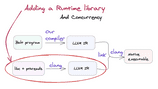
\includegraphics[width=\linewidth]{09_files/runtime-library.png}

%\hypertarget{series-creating-the-bolt-compiler}{%
%\section{Series: Creating the Bolt
%Compiler}\label{series-creating-the-bolt-compiler}}
%
%\begin{itemize}
%\item
%  { Part 1:
%  }\href{https://mukulrathi.com/create-your-own-programming-language/intro-to-compiler/}{How
%  I wrote my own "proper" programming language}
%\item
%  { Part 2:
%  }\href{https://mukulrathi.com/create-your-own-programming-language/compiler-engineering-structure/}{So
%  how do you structure a compiler project?}
%\item
%  { Part 3:
%  }\href{https://mukulrathi.com/create-your-own-programming-language/parsing-ocamllex-menhir/}{Writing
%  a Lexer and Parser using OCamllex and Menhir}
%\item
%  { Part 4:
%  }\href{https://mukulrathi.com/create-your-own-programming-language/intro-to-type-checking/}{An
%  accessible introduction to type theory and implementing a
%  type-checker}
%\item
%  { Part 5:
%  }\href{https://mukulrathi.com/create-your-own-programming-language/data-race-dataflow-analysis/}{A
%  tutorial on liveness and alias dataflow analysis}
%\item
%  { Part 6:
%  }\href{https://mukulrathi.com/create-your-own-programming-language/lower-language-constructs-to-llvm/}{Desugaring
%  - taking our high-level language and simplifying it!}
%\item
%  { Part 7:
%  }\href{https://mukulrathi.com/create-your-own-programming-language/protobuf-ocaml-cpp-tutorial/}{A
%  Protobuf tutorial for OCaml and C++}
%\item
%  { Part 8:
%  }\href{https://mukulrathi.com/create-your-own-programming-language/llvm-ir-cpp-api-tutorial/}{A
%  Complete Guide to LLVM for Programming Language Creators}
%\item
%  \textbf{Part 9: Implementing Concurrency and our Runtime Library}
%\item
%  { Part 10:
%  }\href{https://mukulrathi.com/create-your-own-programming-language/generics-parametric-polymorphism/}{Generics
%  - adding polymorphism to Bolt}
%\item
%  { Part 11:
%  }\href{https://mukulrathi.com/create-your-own-programming-language/inheritance-method-overriding-vtable/}{Adding
%  Inheritance and Method Overriding to Our Language}
%\end{itemize}
%
%\begin{center}\rule{0.5\linewidth}{0.5pt}\end{center}

\hypertarget{the-role-of-a-runtime-library}{%
\section{\texorpdfstring{\protect\hyperlink{the-role-of-a-runtime-library}{}The
Role of a Runtime
Library}{The Role of a Runtime Library}}\label{the-role-of-a-runtime-library}}

Up till now, we've translated constructs in our language Bolt directly
into LLVM IR instructions. The biggest misconception I had with
concurrency was that it worked in the same manner. That there was some
\texttt{spawn} instruction that compilers could emit that would create a
new thread. This isn't the case. LLVM doesn't have a single instruction
to create threads for you. Why not, you ask? What's so special about
threads?

Creating a thread is a complex routine of instructions that are
\textbf{platform-specific}. Threads are managed by the OS kernel, so
creating a thread involves creating system calls following that
platform's conventions.

LLVM draws a line here. There's a limit to how much functionality LLVM
can provide without itself becoming \emph{huge}. Just think of the
variety of platforms out there that it would have to support, from
embedded systems to mobile to the different desktop OSs.

Enter your \textbf{runtime library}. Your language's runtime library
provides the \emph{implementation} for these routines that interact with
the platform / runtime environment. The compiler inserts calls to these
runtime library functions when compiling our Bolt program. Once we have
our compiled LLVM IR, we \textbf{link} in the runtime library function
implementations, so the executable can call these.

You know what the best part is about compiling to LLVM IR? We don't have
to write our own runtime library. C compiles to LLVM IR. Let's just use
C functions to bootstrap our runtime library and \texttt{clang} to link
them in!

So which kinds of functions are present in our runtime library?

\begin{itemize}
\tightlist
\item
  I/O e.g. \texttt{printf}
\item
  Memory management. (Remember in the previous post I mentioned that the
  LLVM didn't provide a heap.) Either implemented manually
  (\texttt{malloc} and \texttt{free}) or through a garbage collection
  algorithm (e.g. \emph{mark-and-sweep}).
\item
  And of course \textbf{threads} via the C \texttt{pthread} API. Pthread
  is short for \href{https://en.wikipedia.org/wiki/POSIX_Threads}{POSIX
  Thread}, a standardised API for these thread system calls.
\end{itemize}

We aren't just limited to the functions provided by C. We can write our
own C functions and link them in using the techniques described in this
post.

We'll look at \texttt{printf}

\hypertarget{recap-llvm-module}{%
\section{\texorpdfstring{\protect\hyperlink{recap-llvm-module}{}Recap:
LLVM Module}{Recap: LLVM Module}}\label{recap-llvm-module}}

Here's a quick sketch of the structure of an LLVM module (from the
\href{https://mukulrathi.com/create-your-own-programming-language/llvm-ir-cpp-api-tutorial/}{previous
post}). As the diagram shows, the part of the module we're interested in
is the \textbf{function declarations}. To use a C library function, we
need to insert its function signature in our module's function
declarations symbol table.

{
\href{https://mukulrathi.com/static/e21edb9623d8fb7bc23f57db23b93cf8/cad61/module.png}{{}
\includegraphics[width=\linewidth]{09_files/module.png}} }

\hypertarget{printf}{%
\section{\texorpdfstring{\protect\hyperlink{printf}{}Printf}{Printf}}\label{printf}}

Let's warm up with \texttt{printf}. The C function type signature is:

%Copy

\begin{lstlisting}[language=C]
int printf ( const char* format, ... );
\end{lstlisting}

To translate this C type signature to an LLVM \texttt{FunctionType}:

\begin{itemize}
\tightlist
\item
  drop the \texttt{const} qualifier
\item
  Convert C types to equivalent LLVM types: \texttt{int} and
  \texttt{char} map to \texttt{i32} and \texttt{i8} respectively
\item
  the \texttt{...} indicates \texttt{printf} is variadic. So the LLVM
  API code is as follows:
\end{itemize}

%{
%\href{https://github.com/mukul-rathi/bolt/blob/master/src/llvm-backend/llvm_ir_codegen/extern_functions_codegen.cc\#L17-L21}{extern\_functions\_codegen.cc}}
%
%Copy

\begin{lstlisting}[language=C++,caption={extern\_functions\_codegen.cc}]
module->getOrInsertFunction(  "printf",  FunctionType::get(    IntegerType::getInt32Ty(*context),    Type::getInt8Ty(*context)->getPointerTo(),    true /* this is variadic func */  ));
\end{lstlisting}

And the corresponding code to call the \texttt{printf} function:

%{
%\href{https://github.com/mukul-rathi/bolt/blob/master/src/llvm-backend/llvm_ir_codegen/expr_codegen.cc\#L412-L424}{expr\_codegen.cc}}
%
%Copy

\begin{lstlisting}[caption={expr\_codegen.cc},language=C++]
Value *IRCodegenVisitor::codegen(const ExprPrintfIR &expr) {
  Function *printf = module->getFunction("printf");
  std::vector<Value *> printfArgs;
  Value *formatStrVal = builder->CreateGlobalStringPtr(expr.formatStr);
  printfArgs.push_back(formatStrVal);
  // add variadic arguments
  for (auto &arg : expr.arguments) {
    printfArgs.push_back(arg->codegen(*this););
  }
  return builder->CreateCall(printf, printfArgs);
};
\end{lstlisting}

\href{https://llvm.org/doxygen/classllvm_1_1IRBuilderBase.html\#abd2f5469db2235e00ac6df61fe766c85}{CreateGlobalStringPtr}
is a useful \texttt{IRBuilder} method that takes in a string and returns
an \texttt{i8*} pointer (so we have a argument of the right type).

\hypertarget{the-bolt-memory-model}{%
\section{\texorpdfstring{\protect\hyperlink{the-bolt-memory-model}{}The
Bolt Memory Model}{The Bolt Memory Model}}\label{the-bolt-memory-model}}

Each thread has \textbf{its own stack}. To share objects between
threads, we'll introduce a \textbf{global heap} of objects. We'll use
the stack to store primitives like ints, bools and to store pointers to
objects on the heap.

{
\href{https://mukulrathi.com/static/f9e2f9b192e5a29e4bca4304ec811151/b4904/hardware-threads.png}{{}
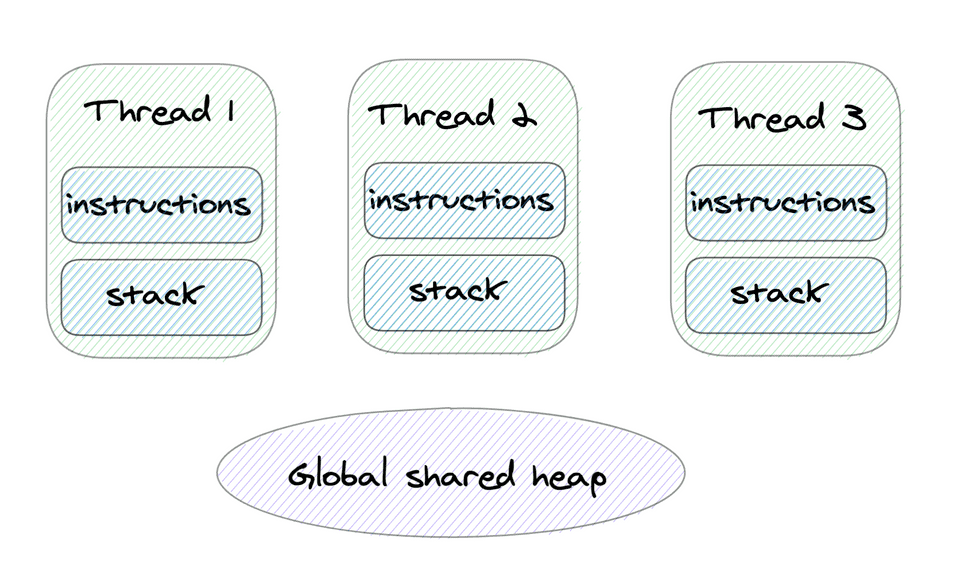
\includegraphics[width=\linewidth]{09_files/hardware-threads.png}} }

{
\href{https://mukulrathi.com/static/ff99489ea7fb99d5a54e6d5a32342340/e53e8/stack-heap.png}{{}
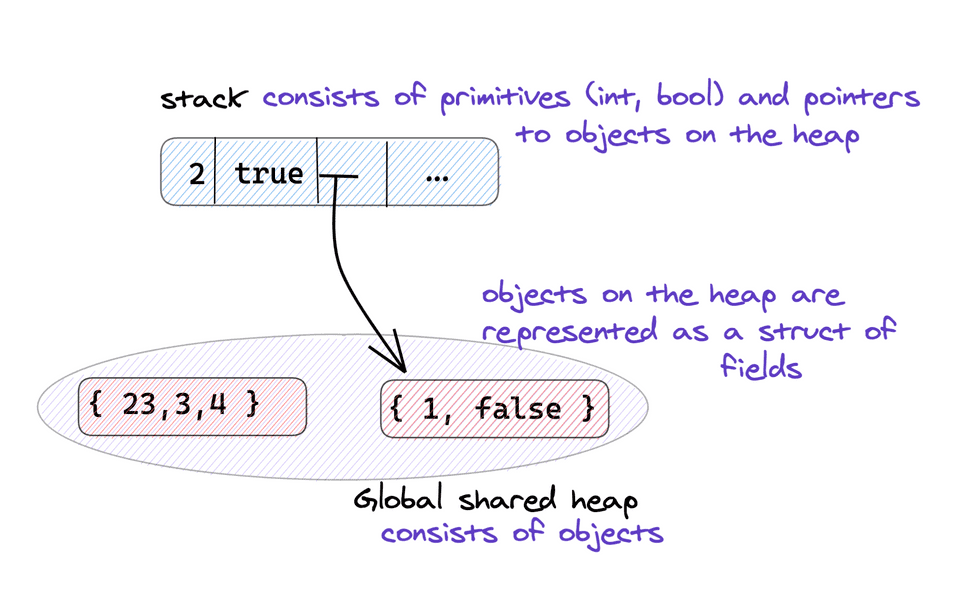
\includegraphics[width=\linewidth]{09_files/stack-heap.png}} }

\hypertarget{malloc}{%
\subsection{\texorpdfstring{\protect\hyperlink{malloc}{}Malloc}{Malloc}}\label{malloc}}

We can use \texttt{malloc} to allocate objects to the heap. (This is
what C++`s \texttt{new} keyword does under the hood!)

The type signature for \texttt{malloc} is as follows:

%Copy

\begin{lstlisting}[language=C]
void *malloc(size_t size);
\end{lstlisting}

Converting this to the equivalent LLVM IR types, \texttt{void\ *} and
\texttt{size\_t} map to \texttt{i8\ *} and \texttt{i64}. The LLVM API
code falls out once you've determined the LLVM types.

%{
%\href{https://github.com/mukul-rathi/bolt/blob/master/src/llvm-backend/llvm_ir_codegen/extern_functions_codegen.cc\#L23-L32}{extern\_functions\_codegen.cc}}
%
%Copy

\begin{lstlisting}[caption={extern\_functions\_codegen.cc},language=C++]
Type *voidPtrTy = Type::getInt8Ty(*context)->getPointerTo();
module->getOrInsertFunction(
  "malloc",  FunctionType::get(
    voidPtrTy,
    IntegerType::getInt64Ty(*context),
    /* has variadic args */ false  ));
\end{lstlisting}

There is just one issue though. When we create a \texttt{struct} on the
heap, \texttt{malloc} requires us to specify the number of bytes we want
to allocate. However the size of that \texttt{struct} is
machine-specific information (it depends on the size of datatype, struct
padding etc.). How do we do this in LLVM IR, which is
machine-independent?

We can compute this through the following \emph{hack}. We know that an
array of structs of type \texttt{Foo} is just a contiguous block of
memory. Pointers to adjacent indices are \texttt{size(Foo)} bytes apart.
Therefore, if we start an array at address \texttt{0x0000} (the special
\texttt{NULL} address) then the first index of the array is at address
\texttt{size(Foo)}.

{
\href{https://mukulrathi.com/static/3ffd7d3a6019e3375f7834e25b4853f8/95fa1/malloc-size.png}{{}
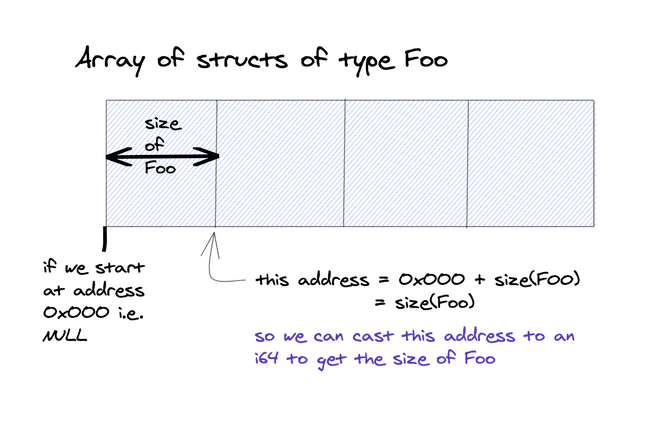
\includegraphics[width=\linewidth]{09_files/malloc-size.png}} }

We can use the \texttt{getelementptr} (GEP) instruction to compute this
array address, and pass in the base pointer of the array as the
\texttt{null} value. You might be thinking, hold on, this array doesn't
exist. Won't this cause a seg fault?

Remember, the role of the GEP instruction is just to calculate pointer
offsets. Not to check if the resultant pointer is valid. Not to actually
access the memory. Just to perform this calculation. No memory access =
no seg fault.

%{
%\href{https://github.com/mukul-rathi/bolt/blob/master/src/llvm-backend/llvm_ir_codegen/expr_codegen.cc\#L74-L83}{expr\_codegen.cc}}
%
%Copy

\begin{lstlisting}[language=C++,caption={expr\_codegen.cc}]
// calculate index of array[1] using GEP instructionValue *objDummyPtr = builder->CreateConstGEP1_64(    Constant::getNullValue(objType->getPointerTo()), 1, "objsize");// cast to i64 for mallocValue *objSize =    builder->CreatePointerCast(objDummyPtr,Type::getInt64Ty(*context));
\end{lstlisting}

We pass \texttt{objSize} to \texttt{malloc}. \texttt{malloc} returns a
\texttt{void\ *} pointer, however since we will later want to access the
struct's fields, we need to cast the type to \texttt{objType*}.
Remember, LLVM needs explicit types!

%{
%\href{https://github.com/mukul-rathi/bolt/blob/master/src/llvm-backend/llvm_ir_codegen/expr_codegen.cc\#L74-L83}{expr\_codegen.cc}}
%
%Copy

\begin{lstlisting}[language=C++,caption={expr\_codegen.cc}]
// allocate the object on the heap
Value *objVoidPtr =
    builder->CreateCall(module->getFunction("malloc"), objSize);
// cast (void *)  to  (objType *)
Value *obj =    builder->CreatePointerCast(objVoidPtr, objType->getPointerTo());
\end{lstlisting}

\hypertarget{bonus-garbage-collection}{%
\subsection{\texorpdfstring{\protect\hyperlink{bonus-garbage-collection}{}Bonus:
Garbage
Collection}{Bonus: Garbage Collection}}\label{bonus-garbage-collection}}

Swap out \texttt{malloc} for \texttt{GC\ malloc}. If we use
\href{https://linux.die.net/man/3/gc}{GC\_malloc}, we get garbage
collection for free! How cool is that?! We don't need to \texttt{free()}
our object.

If you want to implement your own garbage collector,
\href{https://llvm.org/docs/GarbageCollection.html}{check this LLVM page
out}.

\hypertarget{implementing-hardware-threads-with-pthreads}{%
\section{\texorpdfstring{\protect\hyperlink{implementing-hardware-threads-with-pthreads}{}Implementing
Hardware Threads with
Pthreads}{Implementing Hardware Threads with Pthreads}}\label{implementing-hardware-threads-with-pthreads}}

So far we've looked at \texttt{printf} and \texttt{malloc}. We've found
that the biggest hurdle to declaring their function signatures is
translating C types to LLVM IR types. Once you have the LLVM IR types,
everything falls out. With the \texttt{pthread} API the process is the
same, only the translation from C types to LLVM IR types is a little
more involved.

\hypertarget{understanding-the-pthread-api}{%
\subsection{\texorpdfstring{\protect\hyperlink{understanding-the-pthread-api}{}Understanding
the Pthread
API}{Understanding the Pthread API}}\label{understanding-the-pthread-api}}

The two functions we'd like to use to create and join threads are
\href{https://man7.org/linux/man-pages/man3/pthread_create.3.html}{pthread\_create}
and
\href{https://man7.org/linux/man-pages/man3/pthread_join.3.html}{pthread\_join}.
The linked Linux manual pages give a full description of the functions,
but they are a bit dense.

Let's unpack the relevant information, starting with the function
signatures:

%Copy

\begin{lstlisting}[language=C]
int pthread_create(pthread_t *thread, const pthread_attr_t *attr,
                          void *(*start_routine) (void *), void *arg);
int pthread_join(pthread_t thread, void **retval);
\end{lstlisting}

Both \texttt{pthread\_create} and \texttt{pthread\_join} are idiomatic C
functions in that:

\begin{itemize}
\tightlist
\item
  they return an \texttt{int}, where the value \texttt{0} = success and
  other values = error codes.
\item
  to return additional values e.g a \texttt{val} of type \texttt{Foo},
  we pass in a \emph{pointer} \texttt{p} of type \texttt{Foo*} as an
  argument. The function will update the pointer's value to that
  returned value (\texttt{*p=val}). We can then access the returned
  value by dereferencing the pointer (\texttt{*p}).
  \href{https://www.ibm.com/support/knowledgecenter/SSLTBW_2.4.0/com.ibm.zos.v2r4.cbclx01/pass_by_pointer.htm}{See
  this tutorial} if you're not familiar with this
  \emph{``pass-by-pointer''} pattern.
\end{itemize}

If you're not familiar with C pointer syntax,
\texttt{void\ *(*start\_routine)\ (void\ *)} is quite a mouthful. This
says \texttt{start\_routine} is a pointer to a function that takes in a
\texttt{void\ *} argument and returns a \texttt{void\ *} value.
\texttt{void\ *} is the generic type representing \emph{any} pointer
(it's super flexible - we can cast it to any type we'd like e.g.
\texttt{int\ *} or \texttt{Foo\ *}).

\texttt{pthread\_create} creates a thread, which will asynchronously
execute the function pointed to by \texttt{start\_routine} with the
\texttt{arg} argument. The opaque \texttt{pthread\_t} type represents a
handle to a thread object (can think of it like a thread id ). We pass a
\texttt{pthread\_t\ *} pointer, and \texttt{pthread\_create} will assign
the \texttt{pthread\_t} handle corresponding to the created thread to
this object. The opaque \texttt{pthread\_attr\_t} type represents any
attributes we want the thread to have. The \texttt{pthread\_attr\_t\ *}
parameter lets us specify the attributes we want the created thread to
have. Passing \texttt{NULL} will initialise the thread with default
attributes, which is good enough for us.

We pass the \texttt{pthread\_t} handle to \texttt{pthread\_join} to tell
it which thread we are joining (waiting on to finish).
\texttt{pthread\_join} updates the \texttt{void\ **} pointer parameter
with the \texttt{void\ *} return value of \texttt{start\_routine(arg)}
executing on that thread. We can pass \texttt{NULL} if we don't want
this return value.

Here's an
\href{https://timmurphy.org/2010/05/04/pthreads-in-c-a-minimal-working-example/}{excellent
minimal C example} that demonstrates the use of Pthreads.

\hypertarget{translating-pthread-types-into-llvm-ir}{%
\subsection{\texorpdfstring{\protect\hyperlink{translating-pthread-types-into-llvm-ir}{}Translating
Pthread types into LLVM
IR}{Translating Pthread types into LLVM IR}}\label{translating-pthread-types-into-llvm-ir}}

We've seen \texttt{int} and \texttt{void\ *} before: they may to
\texttt{i32} and \texttt{i8*}. \texttt{void\ **} follows as
\texttt{i8*}. We're in a bit of a pickle with \texttt{pthread\_t} and
\texttt{pthread\_attr\_t} as their type definitions are opaque.

Aw shucks, we're stuck. The solution (as with most cases when you're
stuck with LLVM IR) is to \textbf{experiment in C and look at the
compiled LLVM IR output}.

We can compile that
\href{https://timmurphy.org/2010/05/04/pthreads-in-c-a-minimal-working-example/}{excellent
minimal C example} to LLVM IR using \texttt{clang}. The command to do
this for a \texttt{foo.c} file is:

%Copy

\begin{verbatim}
clang -S -emit-llvm -O1 foo.c
\end{verbatim}

The Clang LLVM IR output is quite messy. The best way to read the output
is to find the lines of LLVM IR that correspond to the interesting lines
of code in the C program, and ignore the noise around them. More
information about experimenting with C and C++ to understand LLVM IR in
this
\href{https://www.reddit.com/r/programming/comments/kjjijf/a_complete_guide_to_llvm_for_programming_language/gh2dnnj?utm_source=share\&utm_medium=web2x\&context=3}{excellent
Reddit comment}.

For us, the interesting lines are those that allocate a
\texttt{pthread\_t} stack variable, and the \texttt{pthread\_create} and
\texttt{pthread\_join} calls:

%Copy
\begin{lstlisting}[language=C,caption={C}]
// C
pthread_t inc_x_thread;
...
pthread_create(&inc_x_thread, NULL, inc_x, &x)
...
pthread_join(inc_x_thread, NULL)
\end{lstlisting}

\begin{lstlisting}[language=llvm,caption={LLVM IR}]
%4 = alloca %struct._opaque_pthread_t*, align 8...
%9 = call i32 @pthread_create(%struct._opaque_pthread_t** %4, %struct._opaque_pthread_attr_t* null, i8* (i8*)* @inc_x, i8* %8)...
%23 = call i32 @pthread_join(%struct._opaque_pthread_t* %22, i8** null)
\end{lstlisting}


If we match up our type definitions for the functions:

%Copy

\begin{lstlisting}[language=llvm]
// C type -> LLVM IR 
typepthread_t = %struct._opaque_pthread_t*pthread_attr_t = %struct._opaque_pthread_attr_t
\end{lstlisting}

Great, we've determined \texttt{pthread\_t} is a pointer to a struct of
type \texttt{\%struct.\_opaque\_pthread\_t}. What's the type of this
struct? Let's look at the type definitions defined earlier in the file:

%Copy

\begin{lstlisting}[language=llvm]
struct.__sFILE = type { i8*, i32, i32, i16, i16, %struct.__sbuf, i32, i8*, i32(i8*)*, i32 (i8*, i8*, i32)*, i64 (i8*, i64, i32)*, i32 (i8*, i8*, i32)*, %struct.__sbuf, %struct.__sFILEX*, i32, [3 x i8], [1 x i8], %struct.__sbuf, i32, i64 }%struct.__sFILEX = type opaque%struct.__sbuf = type { i8*, i32 }%struct._opaque_pthread_t = type { i64, %struct.__darwin_pthread_handler_rec*, [8176 x i8] }%struct.__darwin_pthread_handler_rec = type { void (i8*)*, i8*, %struct.__darwin_pthread_handler_rec* }%struct._opaque_pthread_attr_t = type { i64, [56 x i8] }
\end{lstlisting}

Yikes, this is a mess. Here's the thing. We don't have to declare the
internals of the \texttt{struct} because we \textbf{aren't using them}
in our program. So just as \texttt{\%struct.\_\_sFILEX} was defined as
an opaque struct above, we can define our own opaque structs. The
\texttt{pthread} library's files will specify the bodies of the struct
types as it actually manipulates their internals.

%Copy

\begin{lstlisting}[language=C++]
Type *pthread_t = StructType::create(*context, "struct_pthread_t") ->getPointerTo();
Type *pthread_attr_t = StructType::create(*context,"struct_pthread_attr_t")
\end{lstlisting}

The eagle-eyed amongst you might notice these struct names don't match
the names in the file e.g. \texttt{struct\_pthread\_t} vs
\texttt{struct.\_opaque\_pthread\_t}. What gives?

LLVM's types are resolved \textbf{structurally} not by name. So even if
our program has two separate structs \texttt{Foo} and \texttt{Bar}, if
the types of their fields are the same, LLVM will treat them the same.
The name doesn't matter - we can use one in place of the other without
any errors:

%Copy

\begin{lstlisting}[language=llvm]
// Foo == Bar
%Foo = type {i32, i1}
%Bar = type {i32, i1}
\end{lstlisting}

It turns out we can exploit the structural nature of LLVM's type system
to simplify our types further.

See \texttt{pthread\_attr\_t} is only used in one place:
\texttt{pthread\_create}, and there we pass \texttt{NULL} as the
\texttt{pthread\_attr\_t\ *} argument. \texttt{NULL} is the same value
regardless of type, so rather than defining the type
\texttt{pthread\_attr\_t\ *}, we can use \texttt{void\ *} to represent a
generic \texttt{NULL} pointer.

Let's look at \texttt{pthread\_t} next. We know that \texttt{pthread\_t}
is a \textbf{pointer} to some opaque struct, but we never access that
struct anywhere in our program. In fact, the only place
\texttt{pthread\_t}'s type matters is when we're allocating memory on
the stack for it - we need to know the type to know how many bytes to
allocate.

%{
%\href{https://github.com/mukul-rathi/bolt/blob/master/src/llvm-backend/llvm_ir_codegen/expr_codegen.cc\#L401}{expr\_codegen.cc}}
%
%Copy

\begin{lstlisting}[caption={expr\_codegen.cc},language=c++]
Type *pthreadTy = codegenPthreadTy();Value *pthreadPtr =  builder->CreateAlloca(pthreadTy, nullptr, "pthread");
\end{lstlisting}

Here's the thing: \emph{all} pointers have the same size, regardless of
type, as they all store memory addresses. So we can use a generic
pointer type \texttt{void\ *} for \texttt{pthread\_t} too.

%{
%\href{https://github.com/mukul-rathi/bolt/blob/master/src/llvm-backend/llvm_ir_codegen/extern_functions_codegen.cc\#L23-L32}{extern\_functions\_codegen.cc}}
%
%Copy

\begin{lstlisting}[language=C++,caption={extern\_functions\_codegen.cc}]
Type *IRCodegenVisitor::codegenPthreadTy() {   return Type::getInt8Ty(*context)->getPointerTo();}
\end{lstlisting}

The LLVM API code to declare the \texttt{pthread\_create} and
\texttt{pthread\_join} functions is therefore as follows:

%{
%\href{https://github.com/mukul-rathi/bolt/blob/master/src/llvm-backend/llvm_ir_codegen/extern_functions_codegen.cc\#L36-L62}{extern\_functions\_codegen.cc}}
%
%Copy

\begin{lstlisting}[language=C++,caption={extern\_functions\_codegen.cc}]
Type *voidPtrTy = Type::getInt8Ty(*context)->getPointerTo();
Type *pthreadTy = codegenPthreadTy();
Type *pthreadPtrTy = pthreadTy->getPointerTo();
// (void *) fn (void * arg)
FunctionType *funVoidPtrVoidPtrTy = FunctionType::get(  voidPtrTy, ArrayRef<Type *>({voidPtrTy}),  /* has variadic args */ false);
// int pthread_create(pthread_t * thread, const pthread_attr_t * attr,
//                  void * (*start_routine)(void *), void * arg)
// we use a void * in place of pthread_attr_t *
FunctionType *pthreadCreateTy = FunctionType::get(  Type::getInt32Ty(*context),  ArrayRef<Type *>({pthreadPtrTy, voidPtrTy,                (funVoidPtrVoidPtrTy)->getPointerTo(),                voidPtrTy}),  /* has variadic args */ false);
module->getOrInsertFunction("pthread_create", pthreadCreateTy);
// int pthread_join(pthread_t thread, void **value_ptr)
FunctionType *pthreadJoinTy = FunctionType::get(  Type::getInt32Ty(*context),  ArrayRef<Type *>({pthreadTy, voidPtrTy->getPointerTo()}),  /* has variadic args */ false);
module->getOrInsertFunction("pthread_join", pthreadJoinTy);
\end{lstlisting}

\hypertarget{linking-in-the-runtime-library}{%
\section{\texorpdfstring{\protect\hyperlink{linking-in-the-runtime-library}{}Linking
in the Runtime
Library}{Linking in the Runtime Library}}\label{linking-in-the-runtime-library}}

We can use \texttt{clang} to link in the libraries when we compile our
\texttt{foo.ll} file to a \texttt{./foo} executable.

We link in \texttt{pthread} with the \texttt{-pthread} flag.

To link \texttt{GC\_malloc} we need to do two things:

\begin{itemize}
\tightlist
\item
  Include its header files (here they're in the folder
  \texttt{/usr/local/include/gc/}). We use the \texttt{-I} flag to add
  its folder.
\item
  Add the static library \texttt{.a} file:
  \texttt{/usr/local/lib/libgc.a} to the list of files being compiled.
\end{itemize}

{
\href{https://github.com/mukul-rathi/bolt/blob/master/scripts/compile_program.sh}{compile\_program.sh}}

Copy

\begin{verbatim}
clang -O3 -pthread -I/usr/local/include/gc/ foo.ll  /usr/local/lib/libgc.a  -o foo
\end{verbatim}

\hypertarget{generic-approach-to-bootstrapping-with-c-functions}{%
\section{\texorpdfstring{\protect\hyperlink{generic-approach-to-bootstrapping-with-c-functions}{}Generic
Approach to Bootstrapping with C
functions}{Generic Approach to Bootstrapping with C functions}}\label{generic-approach-to-bootstrapping-with-c-functions}}

We've seen 3 examples of C functions used when bootstrapping our runtime
library: \texttt{printf}, \texttt{malloc} and the \texttt{pthread} API.
The generic approach (can skip steps 2 - 4 if you already understand the
function)

\begin{enumerate}
\tightlist
\item
  Get the C function type signature
\item
  Write a minimal example in C
\item
  Compile the C example to LLVM IR and match up the key lines of your
  example with the corresponding lines of IR e.g. function calls
\item
  Simplify any opaque types into more generic types: only define as much
  type info as you need! E.g. if you don't need to know it's a
  \texttt{struct\ *} pointer (because you're not loading it or
  performing GEP instructions), use a \texttt{void\ *}.
\item
  Translate the C types into LLVM IR types
\item
  Declare the function prototype in your module
\item
  Call the function in LLVM IR wherever you need it!
\item
  Link the function in when compiling the executable
\end{enumerate}

\hypertarget{implementing-concurrency-in-bolt}{%
\section{\texorpdfstring{\protect\hyperlink{implementing-concurrency-in-bolt}{}Implementing
Concurrency in
Bolt}{Implementing Concurrency in Bolt}}\label{implementing-concurrency-in-bolt}}

\hypertarget{the-finish-async-construct}{%
\subsection{\texorpdfstring{\protect\hyperlink{the-finish-async-construct}{}The
Finish-Async
Construct}{The Finish-Async Construct}}\label{the-finish-async-construct}}

Bolt uses the \texttt{finish-async} construct for concurrency. The
\texttt{async} keyword spawns (creates) a thread and sets it to execute
the expressions in that \texttt{async} block. The \texttt{finish} block
scopes the lifetime of any threads spawned inside it using the
\texttt{async} keyword - so all spawned threads must \textbf{join} at
the end of the block. This way we've clearly defined the lifetime of our
threads to be that of the \texttt{finish} block.



%Copy

\begin{lstlisting}[caption={{example\_concurrent\_program.bolt}}]
before();
finish{
  async{
    f();
  }
  async{
    g();
    h();
  }
  during();
}
after();
\end{lstlisting}

Illustrating the execution graphically:

\begin{figure}
\centering
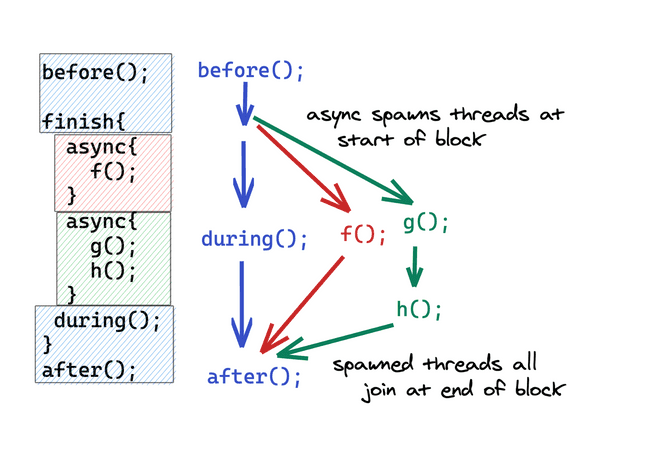
\includegraphics[width=\linewidth]{09_files/finish-async.png}
\caption{A Bolt concurrent program illustrated - each colour represents
a different thread.}
\end{figure}

\hypertarget{creating-our-threads}{%
\subsection{\texorpdfstring{\protect\hyperlink{creating-our-threads}{}Creating
our Threads}{Creating our Threads}}\label{creating-our-threads}}

\hypertarget{compute-free-variables}{%
\paragraph{\texorpdfstring{\protect\hyperlink{compute-free-variables}{}Compute
Free Variables}{Compute Free Variables}}\label{compute-free-variables}}

When inside our \texttt{async} block, we can access any \textbf{objects}
in scope at the start of the \texttt{finish} block (before the
\texttt{async} thread was spawned). For example:

{example\_concurrent\_program.bolt}

Copy

\begin{verbatim}
let a = new Foo();
let b = new Bar();
let y = true;
let z = 2;
finish{
  async{
    // This thread accesses a, b
    let w = 1;
    f(a, b, w);
  }
  ...}
\end{verbatim}

However, there's an issue. In Bolt's memory model, each thread has its
own stack. The \texttt{let\ a\ =\ ...} definition occurs on the main
thread, so the pointer to \texttt{a}'s object is stored on the main
thread's stack. Likewise for \texttt{b}. When we spawn the second thread
using \texttt{async}, this new thread has its own stack, which is empty
(and so doesn't contain \texttt{a} or \texttt{b}).

The first step is to compute the free variables that need to be copied
across to the new stack. Here's a
\href{https://github.com/mukul-rathi/bolt/blob/master/src/frontend/desugaring/desugar_expr.ml\#L140-L141}{link
to the code} if you're interested; we'll skip the details as it's quite
mechanical.
\href{https://mukulrathi.com/create-your-own-programming-language/lower-language-constructs-to-llvm/}{Link
to the previous post on desugaring} if you want to look back at the
desugaring stage.

%Copy

\begin{verbatim}
async{
  //  a, b are free variables
    let w = 1;
    f(a, b, w);
  }
\end{verbatim}

\hypertarget{converting-the-async-block-into-a-function-call}{%
\paragraph{\texorpdfstring{\protect\hyperlink{converting-the-async-block-into-a-function-call}{}Converting
the Async Block into a Function
Call}{Converting the Async Block into a Function Call}}\label{converting-the-async-block-into-a-function-call}}

Now we need to somehow convert this expression into a function that
\texttt{pthread\_create} can run.

%Copy

\begin{verbatim}
async{
    let w = 1;
    f(a, b, w);  }
//  need to convert this to a function
void *asyncFun(void *arg){
  let w = 1;
  f(a, b, w);
  return null;
 // we return null but 
 // you could return the last value instead
}
\end{verbatim}

Since we need all the variables in the function body to be defined, we
need to pass the free variables as arguments to the function:

%Copy

\begin{verbatim}
function void *asyncFun(Foo a, Bar b){
  let w = 1;
  f(a, b, w);
}
let a = new Foo();
let b = new Bar();
let y = true;
let z = 2;
finish{  asyncFun(a, b);  ...}
\end{verbatim}

However, this doesn't match the argument type we're looking for:
\texttt{asyncFun} can only take a \emph{single} \texttt{void*} argument.

The solution: create a \emph{single struct} that contains all of the
values. We can cast the \texttt{struct\ *} to and from a
\texttt{void\ *} pointer to match types.

Copy

\begin{verbatim}
ArgStructType *argStruct = {a, b};// we can cast ArgStructType * to void *asyncFun(argStruct);
\end{verbatim}

Great, now we have the \texttt{void\ *asyncFun(void\ *argStruct)}
function type, as \texttt{pthread\_create} requires.

We need to unpack this inside the function:

%Copy

\begin{verbatim}
function void *asyncFun(void * arg){
  // cast pointer
  ArgStructType *argStruct = (ArgStructType *) arg;
  // unpack variables
  let a = argStruct.a;
  let b = argStruct.b;
  // execute body of function
  let w = 1;
  f(a, b, w);
}
\end{verbatim}

\hypertarget{creating-pthreads}{%
\paragraph{\texorpdfstring{\protect\hyperlink{creating-pthreads}{}Creating
Pthreads}{Creating Pthreads}}\label{creating-pthreads}}

Finally, having defined our arg and our async function, we can invoke
\texttt{pthread\_create}.

The high-level structure of this is as follows:

%{
%\href{https://github.com/mukul-rathi/bolt/blob/master/src/llvm-backend/llvm_ir_codegen/pthread_codegen.cc\#L38-L60}{pthread\_codegen.cc}}
%
%Copy

\begin{lstlisting}[caption={pthread\_codegen.cc},language=C++]
// create async function and argument
  StructType *argStructTy = codegenAsyncFunArgStructType(freeVarList);
  Value *argStruct = codegenAsyncFunArgStruct(asyncExpr, argStructTy);
  Function *asyncFun = codegenAsyncFunction(asyncExpr, argStructTy);
  ...
  // spawn thread
  Function *pthread_create =
      module->getFunction("pthread_create");
  Value *voidPtrNull = Constant::getNullValue(
      Type::getInt8Ty(*context)->getPointerTo());
  Value *args[4] = {
      pthread,
      voidPtrNull,
      asyncFun,
      builder->CreatePointerCast(argStruct, voidPtrTy),  };
  builder->CreateCall(pthread_create, args);
\end{lstlisting}

\texttt{codegenAsyncFunArgStructType}, \texttt{codegenAsyncFunArgStruct}
and \texttt{codegenAsyncFunction} just implement the steps we've
outlined in prose.

\hypertarget{joining-pthreads}{%
\subsection{\texorpdfstring{\protect\hyperlink{joining-pthreads}{}Joining
Pthreads}{Joining Pthreads}}\label{joining-pthreads}}

We join each of the \texttt{pthread\_t} handles for each of the
\texttt{async} expressions' threads.\\
As we mentioned earlier, we aren't returning anything from the
\texttt{asyncFun}, so we can pass in \texttt{NULL} as the second
argument:

%{
%\href{https://github.com/mukul-rathi/bolt/blob/master/src/llvm-backend/llvm_ir_codegen/pthread_codegen.cc\#L14-L25}{pthread\_codegen.cc}}
%
%Copy

\begin{lstlisting}[caption={pthread\_codegen.cc},language=C++]
void IRCodegenVisitor::codegenJoinPThreads(
    const std::vector<Value *> pthreadPtrs) {
  Function *pthread_join =
      module->getFunction("pthread_join");
  Type *voidPtrPtrTy =
      Type::getInt8Ty(*context)->getPointerTo()->getPointerTo();
  for (auto &pthreadPtr : pthreadPtrs) {
    Value *pthread = builder->CreateLoad(pthreadPtr);
    builder->CreateCall(pthread_join,
                        {pthread, Constant::getNullValue(voidPtrPtrTy)});  
  }
\end{lstlisting}

\hypertarget{implementing-finish-async-in-llvm-ir}{%
\subsection{\texorpdfstring{\protect\hyperlink{implementing-finish-async-in-llvm-ir}{}Implementing
Finish-Async in LLVM
IR}{Implementing Finish-Async in LLVM IR}}\label{implementing-finish-async-in-llvm-ir}}

Now we've talked about how we create threads and how we join threads, we
can give the overall code generation for the \texttt{finish-async}
concurrency construct:

%{
%\href{https://github.com/mukul-rathi/bolt/blob/master/src/llvm-backend/llvm_ir_codegen/expr_codegen.cc\#L388-L408}{expr\_codegen.cc}}
%
%Copy

\begin{lstlisting}[caption={expr\_codegen.cc},language=C++]
Value *IRCodegenVisitor::codegen(
    const ExprFinishAsyncIR &finishAsyncExpr) {
  std::vector<Value *> pthreadPtrs;
  // spawn each of the pthreads
  for (auto &asyncExpr : finishAsyncExpr.asyncExprs) {
    Type *pthreadTy = codegenPthreadTy();
    Value *pthreadPtr =
        builder->CreateAlloca(pthreadTy, nullptr, Twine("pthread"));
    pthreadPtrs.push_back(pthreadPtr);
    codegenCreatePThread(pthreadPtr, *asyncExpr);  };

  // execute the current thread's expressions
  Value *exprVal;
  for (auto &expr : finishAsyncExpr.currentThreadExpr) {
    exprVal = expr->codegen(*this);
  }
  // join the threads at the end of the finish block
  codegenJoinPThreads(pthreadPtrs);
  return exprVal;
\end{lstlisting}

\hypertarget{wrap-up}{%
\section{\texorpdfstring{\protect\hyperlink{wrap-up}{}Wrap
Up}{Wrap Up}}\label{wrap-up}}

In this post, we've looked at the role of a runtime library and how we
can bootstrap our Bolt runtime with C functions. We looked at a generic
way of adding C function declarations to our modules, and then link them
with our compiled \texttt{.ll} file. I'd encourage you to add further C
function to the runtime library. e.g. \texttt{scanf} to go with our
\texttt{printf} function.

The second half of this post was a deep-dive into how Bolt does
concurrency. We've used \texttt{pthread} to spawn a hardware thread for
each \texttt{async} expression. An extension might be to use a
\href{https://en.wikipedia.org/wiki/Thread_pool\#:~:text=In\%20computer\%20programming\%2C\%20a\%20thread,execution\%20by\%20the\%20supervising\%20program.}{thread
pool} instead!

%\hypertarget{share-this-on-twitter}{%
%\subsection{Share This On Twitter}\label{share-this-on-twitter}}
%
%If you liked this post, please consider sharing it with your network. If
%you have any questions, tweet away and I'll answer :) I also tweet when
%new posts drop!
%
%\textbf{PS:} I also share helpful tips and links as I'm learning - so
%you get them \textbf{well before} they make their way into a post!
%
%\hypertarget{series-creating-the-bolt-compiler-1}{%
%\section{Series: Creating the Bolt
%Compiler}\label{series-creating-the-bolt-compiler-1}}
%
%\begin{itemize}
%\item
%  { Part 1:
%  }\href{https://mukulrathi.com/create-your-own-programming-language/intro-to-compiler/}{How
%  I wrote my own "proper" programming language}
%\item
%  { Part 2:
%  }\href{https://mukulrathi.com/create-your-own-programming-language/compiler-engineering-structure/}{So
%  how do you structure a compiler project?}
%\item
%  { Part 3:
%  }\href{https://mukulrathi.com/create-your-own-programming-language/parsing-ocamllex-menhir/}{Writing
%  a Lexer and Parser using OCamllex and Menhir}
%\item
%  { Part 4:
%  }\href{https://mukulrathi.com/create-your-own-programming-language/intro-to-type-checking/}{An
%  accessible introduction to type theory and implementing a
%  type-checker}
%\item
%  { Part 5:
%  }\href{https://mukulrathi.com/create-your-own-programming-language/data-race-dataflow-analysis/}{A
%  tutorial on liveness and alias dataflow analysis}
%\item
%  { Part 6:
%  }\href{https://mukulrathi.com/create-your-own-programming-language/lower-language-constructs-to-llvm/}{Desugaring
%  - taking our high-level language and simplifying it!}
%\item
%  { Part 7:
%  }\href{https://mukulrathi.com/create-your-own-programming-language/protobuf-ocaml-cpp-tutorial/}{A
%  Protobuf tutorial for OCaml and C++}
%\item
%  { Part 8:
%  }\href{https://mukulrathi.com/create-your-own-programming-language/llvm-ir-cpp-api-tutorial/}{A
%  Complete Guide to LLVM for Programming Language Creators}
%\item
%  \textbf{Part 9: Implementing Concurrency and our Runtime Library}
%\item
%  { Part 10:
%  }\href{https://mukulrathi.com/create-your-own-programming-language/generics-parametric-polymorphism/}{Generics
%  - adding polymorphism to Bolt}
%\item
%  { Part 11:
%  }\href{https://mukulrathi.com/create-your-own-programming-language/inheritance-method-overriding-vtable/}{Adding
%  Inheritance and Method Overriding to Our Language}
%\end{itemize}
%
%\begin{itemize}
%\item ~
%  \hypertarget{a-complete-guide-to-llvm-for-programming-language-creators}{%
%  \subsection{\texorpdfstring{\href{https://mukulrathi.com/create-your-own-programming-language/llvm-ir-cpp-api-tutorial/}{←
%  A Complete Guide to LLVM for Programming Language
%  Creators}}{← A Complete Guide to LLVM for Programming Language Creators}}\label{a-complete-guide-to-llvm-for-programming-language-creators}}
%\item ~
%  \hypertarget{write-it-and-they-will-eventually-come}{%
%  \subsection{\texorpdfstring{\href{https://mukulrathi.com/2020-blog-review/}{Write
%  It and They Will (Eventually) Come
%  →}}{Write It and They Will (Eventually) Come →}}\label{write-it-and-they-will-eventually-come}}
%\end{itemize}
%
%\hypertarget{table-of-contents}{%
%\section{Table of Contents}\label{table-of-contents}}
%
%\href{https://mukulrathi.com/create-your-own-programming-language/concurrency-runtime-language-tutorial/\#top-of-page}{}
%
%\hypertarget{implementing-concurrency-and-our-runtime-library}{%
%\subsection{Implementing Concurrency and our Runtime
%Library}\label{implementing-concurrency-and-our-runtime-library}}
%
%\begin{itemize}
%\item
%  \href{https://mukulrathi.com/create-your-own-programming-language/concurrency-runtime-language-tutorial/\#the-role-of-a-runtime-library}{}
%
%  \hypertarget{the-role-of-a-runtime-library-1}{%
%  \subsection{The Role of a Runtime
%  Library}\label{the-role-of-a-runtime-library-1}}
%\item
%  \href{https://mukulrathi.com/create-your-own-programming-language/concurrency-runtime-language-tutorial/\#recap-llvm-module}{}
%
%  \hypertarget{recap-llvm-module-1}{%
%  \subsection{Recap: LLVM Module}\label{recap-llvm-module-1}}
%\item
%  \href{https://mukulrathi.com/create-your-own-programming-language/concurrency-runtime-language-tutorial/\#printf}{}
%
%  \hypertarget{printf-1}{%
%  \subsection{Printf}\label{printf-1}}
%\item
%  \href{https://mukulrathi.com/create-your-own-programming-language/concurrency-runtime-language-tutorial/\#the-bolt-memory-model}{}
%
%  \hypertarget{the-bolt-memory-model-1}{%
%  \subsection{The Bolt Memory Model}\label{the-bolt-memory-model-1}}
%
%  \begin{itemize}
%  \item
%    \href{https://mukulrathi.com/create-your-own-programming-language/concurrency-runtime-language-tutorial/\#malloc}{}
%
%    \hypertarget{malloc-1}{%
%    \subsection{Malloc}\label{malloc-1}}
%  \item
%    \href{https://mukulrathi.com/create-your-own-programming-language/concurrency-runtime-language-tutorial/\#bonus-garbage-collection}{}
%
%    \hypertarget{bonus-garbage-collection-1}{%
%    \subsection{Bonus: Garbage
%    Collection}\label{bonus-garbage-collection-1}}
%  \end{itemize}
%\item
%  \href{https://mukulrathi.com/create-your-own-programming-language/concurrency-runtime-language-tutorial/\#implementing-hardware-threads-with-pthreads}{}
%
%  \hypertarget{implementing-hardware-threads-with-pthreads-1}{%
%  \subsection{Implementing Hardware Threads with
%  Pthreads}\label{implementing-hardware-threads-with-pthreads-1}}
%
%  \begin{itemize}
%  \item
%    \href{https://mukulrathi.com/create-your-own-programming-language/concurrency-runtime-language-tutorial/\#understanding-the-pthread-api}{}
%
%    \hypertarget{understanding-the-pthread-api-1}{%
%    \subsection{Understanding the Pthread
%    API}\label{understanding-the-pthread-api-1}}
%  \item
%    \href{https://mukulrathi.com/create-your-own-programming-language/concurrency-runtime-language-tutorial/\#translating-pthread-types-into-llvm-ir}{}
%
%    \hypertarget{translating-pthread-types-into-llvm-ir-1}{%
%    \subsection{Translating Pthread types into LLVM
%    IR}\label{translating-pthread-types-into-llvm-ir-1}}
%  \end{itemize}
%\item
%  \href{https://mukulrathi.com/create-your-own-programming-language/concurrency-runtime-language-tutorial/\#linking-in-the-runtime-library}{}
%
%  \hypertarget{linking-in-the-runtime-library-1}{%
%  \subsection{Linking in the Runtime
%  Library}\label{linking-in-the-runtime-library-1}}
%\item
%  \href{https://mukulrathi.com/create-your-own-programming-language/concurrency-runtime-language-tutorial/\#generic-approach-to-bootstrapping-with-c-functions}{}
%
%  \hypertarget{generic-approach-to-bootstrapping-with-c-functions-1}{%
%  \subsection{Generic Approach to Bootstrapping with C
%  functions}\label{generic-approach-to-bootstrapping-with-c-functions-1}}
%\item
%  \href{https://mukulrathi.com/create-your-own-programming-language/concurrency-runtime-language-tutorial/\#implementing-concurrency-in-bolt}{}
%
%  \hypertarget{implementing-concurrency-in-bolt-1}{%
%  \subsection{Implementing Concurrency in
%  Bolt}\label{implementing-concurrency-in-bolt-1}}
%
%  \begin{itemize}
%  \item
%    \href{https://mukulrathi.com/create-your-own-programming-language/concurrency-runtime-language-tutorial/\#the-finish-async-construct}{}
%
%    \hypertarget{the-finish-async-construct-1}{%
%    \subsection{The Finish-Async
%    Construct}\label{the-finish-async-construct-1}}
%  \item
%    \href{https://mukulrathi.com/create-your-own-programming-language/concurrency-runtime-language-tutorial/\#creating-our-threads}{}
%
%    \hypertarget{creating-our-threads-1}{%
%    \subsection{Creating our Threads}\label{creating-our-threads-1}}
%  \item
%    \href{https://mukulrathi.com/create-your-own-programming-language/concurrency-runtime-language-tutorial/\#joining-pthreads}{}
%
%    \hypertarget{joining-pthreads-1}{%
%    \subsection{Joining Pthreads}\label{joining-pthreads-1}}
%  \item
%    \href{https://mukulrathi.com/create-your-own-programming-language/concurrency-runtime-language-tutorial/\#implementing-finish-async-in-llvm-ir}{}
%
%    \hypertarget{implementing-finish-async-in-llvm-ir-1}{%
%    \subsection{Implementing Finish-Async in LLVM
%    IR}\label{implementing-finish-async-in-llvm-ir-1}}
%  \end{itemize}
%\item
%  \href{https://mukulrathi.com/create-your-own-programming-language/concurrency-runtime-language-tutorial/\#wrap-up}{}
%
%  \hypertarget{wrap-up-1}{%
%  \subsection{Wrap Up}\label{wrap-up-1}}
%\end{itemize}
%
%© Mukul Rathi 2023
%
%\hypertarget{gatsby-announcer}{}
%Navigated to Implementing Concurrency and our Runtime Library

%\hypertarget{___gatsby}{}
%\hypertarget{gatsby-focus-wrapper}{}
%\href{https://mukulrathi.com/}{}
%
%MUKUL RATHI
%
%\href{https://mukulrathi.com/about-me}{}
%
%About Me
%
%\href{https://mukulrathi.com/blog}{}
%
%Blog
%
%\hypertarget{creating-the-bolt-compiler-part-10}{%
%\subsection{Creating the Bolt Compiler: Part
%10}\label{creating-the-bolt-compiler-part-10}}

\hypertarget{top-of-page}{%
\chapter{Generics - adding polymorphism to Bolt}\label{top-of-page}}

January 23, 2021

%\hypertarget{january-23-2021}{%
%\subsection{January 23, 2021}\label{january-23-2021}}
%
%\hypertarget{min-read}{%
%\subsection{4 min read}\label{min-read}}

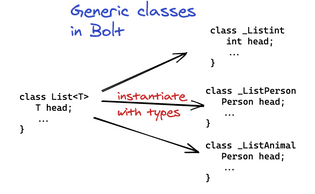
\includegraphics[width=\linewidth]{10_files/generics.png}

%\hypertarget{series-creating-the-bolt-compiler}{%
%\section{Series: Creating the Bolt
%Compiler}\label{series-creating-the-bolt-compiler}}
%
%\begin{itemize}
%\item
%  { Part 1:
%  }\href{https://mukulrathi.com/create-your-own-programming-language/intro-to-compiler/}{How
%  I wrote my own "proper" programming language}
%\item
%  { Part 2:
%  }\href{https://mukulrathi.com/create-your-own-programming-language/compiler-engineering-structure/}{So
%  how do you structure a compiler project?}
%\item
%  { Part 3:
%  }\href{https://mukulrathi.com/create-your-own-programming-language/parsing-ocamllex-menhir/}{Writing
%  a Lexer and Parser using OCamllex and Menhir}
%\item
%  { Part 4:
%  }\href{https://mukulrathi.com/create-your-own-programming-language/intro-to-type-checking/}{An
%  accessible introduction to type theory and implementing a
%  type-checker}
%\item
%  { Part 5:
%  }\href{https://mukulrathi.com/create-your-own-programming-language/data-race-dataflow-analysis/}{A
%  tutorial on liveness and alias dataflow analysis}
%\item
%  { Part 6:
%  }\href{https://mukulrathi.com/create-your-own-programming-language/lower-language-constructs-to-llvm/}{Desugaring
%  - taking our high-level language and simplifying it!}
%\item
%  { Part 7:
%  }\href{https://mukulrathi.com/create-your-own-programming-language/protobuf-ocaml-cpp-tutorial/}{A
%  Protobuf tutorial for OCaml and C++}
%\item
%  { Part 8:
%  }\href{https://mukulrathi.com/create-your-own-programming-language/llvm-ir-cpp-api-tutorial/}{A
%  Complete Guide to LLVM for Programming Language Creators}
%\item
%  { Part 9:
%  }\href{https://mukulrathi.com/create-your-own-programming-language/concurrency-runtime-language-tutorial/}{Implementing
%  Concurrency and our Runtime Library}
%\item
%  \textbf{Part 10: Generics - adding polymorphism to Bolt}
%\item
%  { Part 11:
%  }\href{https://mukulrathi.com/create-your-own-programming-language/inheritance-method-overriding-vtable/}{Adding
%  Inheritance and Method Overriding to Our Language}
%\end{itemize}
%
%\begin{center}\rule{0.5\linewidth}{0.5pt}\end{center}

Onward with more features that any ``proper'' programming language
needs. Today we're implementing \textbf{generics}. Generics allow you to
reuse code for multiple types. Take a \texttt{List} for example. A list
has the same operations regardless of types: it'd be a pain to write out
a new class for each list.

%Copy

\begin{lstlisting}[language=Java]
class ListInt{  ...}
class ListPerson{  ...}
class ListAnimal{  ...}
\end{lstlisting}

The generic class for that would be
\texttt{List\textless{}T\textgreater{}}. We call \texttt{T} the generic
type \emph{parameter}. Think of it like a variable, which we assign a
type to when we instantiate the class:
\texttt{List\textless{}int\textgreater{}()}. Let's build it! We'd like
to compile this program:

%Copy

\begin{lstlisting}[language=Java]
class List<T>{  
    void add(T a){    ...  }  
    T getHead(){    ...  }  
    int size(){    ...  }
}

void main(){  
  let list1 = new List<int>();  
  list1.add(4);  
  ...
}
\end{lstlisting}

\hypertarget{just-give-me-the-code}{%
\section{\texorpdfstring{\protect\hyperlink{just-give-me-the-code}{}Just
give me the
code!}{Just give me the code!}}\label{just-give-me-the-code}}

As ever, the code is in the
\href{https://github.com/mukul-rathi/bolt}{Bolt repo}. The generics are
handled in the
\href{https://github.com/mukul-rathi/bolt/tree/master/src/frontend/typing}{typing}
and
\href{https://github.com/mukul-rathi/bolt/tree/master/src/frontend/desugaring}{desugaring}
stages of the compiler. The code is in the files that contain
\texttt{generics} in their name e.g. \texttt{type\_generics.ml}. You
could even just
\href{https://github.com/mukul-rathi/bolt/search?q=generic}{search
``generic'' in the repo}!

\hypertarget{type-parameters-are-just-like-other-types}{%
\section{\texorpdfstring{\protect\hyperlink{type-parameters-are-just-like-other-types}{}Type
parameters are just like other
types!}{Type parameters are just like other types!}}\label{type-parameters-are-just-like-other-types}}

Rejoice, we don't need to rewrite our type-checker! This tutorial is
much shorter than you think. Here's all that changes in the
type-checker:

\begin{itemize}
\item
  \textbf{Within} our generic class, we can treate our type parameter
  \texttt{T} as an opaque type \texttt{TEGeneric}. So type-check the
  class as before, just don't make any assumptions about \texttt{T}.
\item
  Outside a generic class we can't use generic types \texttt{T}, so
  raise an error if we see that.
\item
  Whenever we use an object instantiated with a type, e.g.
  \texttt{List\textless{}int\textgreater{}}, we can replace all
  occurrences of \texttt{T} with the instantiated type \texttt{int}!
\end{itemize}

That's all that's changed. Seriously!

\hypertarget{treat-the-generic-type-parameter-as-an-opaque-type}{%
\subsection{\texorpdfstring{\protect\hyperlink{treat-the-generic-type-parameter-as-an-opaque-type}{}Treat
the generic type parameter as an opaque
type}{Treat the generic type parameter as an opaque type}}\label{treat-the-generic-type-parameter-as-an-opaque-type}}

We've added to the list of Bolt types a \texttt{TEGeneric} type to
represent this opaque type \texttt{T}.

When we call objects of generic classes, we don't have an object of just
\texttt{List}, it's \texttt{List\textless{}int\textgreater{}},
\texttt{List\textless{}Person\textgreater{}} etc. So we update class
types \texttt{TEClass} to carry around this instantiated type parameter
\texttt{int}, \texttt{Person} etc. if they're generic.
%
%{
%\href{https://github.com/mukul-rathi/bolt/blob/master/src/frontend/ast/ast_types.mli}{ast\_types.ml}}
%
%Copy

\begin{lstlisting}[language=caml,caption={ast\_types.ml}]
type type_expr =  | TEInt  
                 | TEClass   of Class_name.t * type_expr option  
                   (** optionally specify instantiation of type parameter *)  
                 | TEVoid  | TEBool  | TEGeneric
\end{lstlisting}

Next we need to update the \texttt{class\_defn} type to distinguish
between non-generic and generic classes. We define a special type as I
think it's more instructive to see
\texttt{Some\ Generic\ \textbar{}\ None} rather than
\texttt{true\ \textbar{}\ false}. As before, ignore the
\texttt{capability\ list} if you're not interested in the data-race
prevention!
(\href{https://github.com/mukul-rathi/bolt-dissertation/blob/master/dissertation.pdf}{See
my dissertation for a full explanation if you are}).

%{
%\href{https://github.com/mukul-rathi/bolt/blob/master/src/frontend/ast/ast_types.mli}{ast\_types.ml}}
%
%Copy

\begin{lstlisting}[language=caml,caption={ast\_types.ml}]
type generic_type = Generic
\end{lstlisting}

%{
%\href{https://github.com/mukul-rathi/bolt/blob/master/src/frontend/parsing/parsed_ast.ml}{parsed\_ast.ml}}
%
%Copy

\begin{lstlisting}[language=caml,caption={{parsed\_ast.ml}}]
type class_defn = TClass of      Class_name.t      * generic_type option      * capability list (* for data-races (see dissertation) *)      * field_defn list      * method_defn list
\end{lstlisting}

And now, within a generic class \texttt{List}, we instantiate
\texttt{this} to be of type \texttt{List\textless{}T\textgreater{}}
(remember we treat \texttt{T} as an opaque type \texttt{TEGeneric}):
%
%{
%\href{https://github.com/mukul-rathi/bolt/blob/master/src/frontend/typing/type_generics.ml\#L163-L169}{type\_generics.ml}}
%
%Copy

\begin{lstlisting}[language=caml,caption={type\_generics.ml}]
let instantiate_maybe_in_generic_class_this    (Parsed_ast.TClass (class_name, maybe_in_generic_class, _, _, _, _)) =  
   let maybe_type_param =    (* use generic type T inside class *)    
     match maybe_in_generic_class with 
      Some Generic -> Some TEGeneric 
     | None -> None in  (Var_name.of_string "this", TEClass (class_name, maybe_type_param))
\end{lstlisting}

And then the type-checking works as before!

\hypertarget{check-usage-of-generic-types}{%
\subsection{\texorpdfstring{\protect\hyperlink{check-usage-of-generic-types}{}Check
usage of generic
types}{Check usage of generic types}}\label{check-usage-of-generic-types}}

Outside a generic class we can't use generic types. I hate to bore you,
this code is quite mechanical - it's a lot of recursively going through
each of the subexpressions. For a class, check each of the fields,
methods etc. For a function, check its type signature and then its body.
And so on.

Here's a snippet of a function that checks a type. If we're in a generic
class it's all fine, otherwise check we aren't using a generic type.
Click the link to the \texttt{type\_generics.ml} file below to see the
full code.

%{
%\href{https://github.com/mukul-rathi/bolt/blob/master/src/frontend/typing/type_generics.ml\#L5-L21}{type\_generics.ml}}
%
%Copy

\begin{lstlisting}[language=caml,caption={type\_generics.ml}]
let rec type_generics_usage_type type_expr maybe_in_generic_class error_prefix_str =
  match maybe_generic with
  | Some Generic -> Ok () (* can have generics in generic class *)
  | None         -> (    (* recursively check there aren't nested uninitialised type parameters *)
    match type_expr with
    | TEInt | TEBool | TEVoid       -> Ok ()
    | TEGeneric                     ->        Error          (Error.of_string             (Fmt.str "%s Type error: Use of generic type but not in a generic class@."                error_prefix_str))
    | TEClass (_, maybe_type_param) -> (
      match maybe_type_param with
      | Some type_param ->          type_generics_usage_type type_param maybe_in_generic_class error_prefix_str
      | None            -> Ok () ) )
\end{lstlisting}

\hypertarget{instantiate-generic-objects}{%
\subsection{\texorpdfstring{\protect\hyperlink{instantiate-generic-objects}{}Instantiate
generic
objects}{Instantiate generic objects}}\label{instantiate-generic-objects}}

We check first that we should be instantiating with a type-parameter. If
we're trying to instantiate a non-generic class with a type param, raise
an Error, and likewise if we haven't provided a concrete type for a
generic class, raise an error. If we do have a generic class, then
recursively replace all instances of a generic type with the concrete
type: the fields and then the methods etc. Again, full details are in
the repo:

%{
%\href{https://github.com/mukul-rathi/bolt/blob/master/src/frontend/typing/type_generics.ml\#L213-L246}{type\_generics.ml}}
%
%Copy

\begin{lstlisting}[language=caml,caption={type\_generics.ml}]
let instantiate_maybe_generic_class_defn maybe_type_param    ( Parsed_ast.TClass        (class_name, maybe_generic, caps, field_defns, method_defns) as    class_defn ) loc =  
match (maybe_generic, maybe_type_param) with  
  | None, None  (* non-generic class *) ->  Ok class_defn
  | None, Some type_param         ->   Error ...
  | Some Generic, None            -> Error ...
  | Some Generic, Some type_param ->   List.map ~f:(instantiate_maybe_generic_field_defn type_param) field_defns      |> fun instantiated_field_defns ->      List.map ~f:(instantiate_maybe_generic_method_defn type_param) method_defns      |> fun instantiated_method_defns ->      Ok        (Parsed_ast.TClass           ( class_name           , maybe_generic           , caps           , instantiated_field_defns           , instantiated_method_defns ))
\end{lstlisting}

\hypertarget{desugaring-generics}{%
\section{\texorpdfstring{\protect\hyperlink{desugaring-generics}{}Desugaring
Generics}{Desugaring Generics}}\label{desugaring-generics}}

Ok, so we've type-checked our generics, and they pass our checks. What
now? What do we tell our LLVM compiler backend to do when it encounters
a \texttt{T}? You can't allocate a ``generic'' block of memory.

So we \emph{desugar} away all mentions of generic types. What the
compiler backend doesn't know about, it doesn't have to deal with.

Remember, we did this for function overloading
\href{https://mukulrathi.com/create-your-own-programming-language/lower-language-constructs-to-llvm/}{in
our desugaring post}:

%Copy

\begin{verbatim}
function int test(int f) {  ...}
function int test(bool b){  ...}
// DESUGARED (name-mangle functions)
function int testi(int f) {  ...}
function int testb(bool b){  ...}
\end{verbatim}

The compiler backend doesn't need to worry about multiple functions with
the same name, because we handled it in the desugaring stage.

Remember how I said it'd be a pain to write out a new class for each
list? It would be \emph{for us}, as we're doing it by hand. It isn't for
the compiler: it can automate it! To avoid any name-clashes, we'll
prepend each compiler-generated class with an \texttt{\_}.

%Copy

\begin{verbatim}
class _Listint{  ...}
class _ListPerson{  ...}
class _ListAnimal{  ...}
\end{verbatim}

So our desugaring stage has 3 steps to handle generics:

\begin{itemize}
\item
  Count all instantiations of generics
\item
  Create a special class for each of the instantiations (identical to
  how we instantiated generic objects earlier)
\item
  Replace each generic class' constructor with its instantiated class.
  So \texttt{List\textless{}int\textgreater{}} goes to the class
  \texttt{\_Listint}.
\end{itemize}

As before, let's dive into the code!

\hypertarget{count-all-instantiations-of-generics}{%
\subsection{\texorpdfstring{\protect\hyperlink{count-all-instantiations-of-generics}{}Count
all instantiations of
generics}{Count all instantiations of generics}}\label{count-all-instantiations-of-generics}}

This is in the \texttt{count\_generics\_instantiations.ml} file in the
repo (creative name I know!).

We go through the code recursively, and every time we see a constructor
with a concrete type param e.g.
\texttt{List\textless{}int\textgreater{}}, we add that instantiation
\texttt{int} to the total instantiations. In the code below,
\texttt{class\_insts} is a list containing pairs
\texttt{(class\_name,\ list\_of\_types\_instantiated\_with)}:

%{
%\href{https://github.com/mukul-rathi/bolt/blob/master/src/frontend/desugaring/count_generics_instantiations.ml\#L7-L21}{count\_generics\_instantiations.ml}}
%
%Copy

\begin{lstlisting}[language=caml,caption={count\_generics\_instantiations.ml}]
let rec count_generics_instantiations_expr class_defns expr class_insts =  match expr with  | Typed_ast.Constructor (_, class_name, maybe_type_param, constructor_args) ->      ( match maybe_type_param with      | Some TEGeneric  -> class_insts (* only consider concrete type params *)      | Some type_param -> add_instantiation class_defns type_param class_name class_insts      | None            -> class_insts )  ... (* recursive calls *)
\end{lstlisting}

An aside: we can be overly conservative with our counting, as if we
instantiate classes that don't actually get used, then LLVM will
optimise them away. So we could have brute-forced all possible
combinations - this would have slowed the compiler down, but it wouldn't
have affected the code output.

\hypertarget{replace-generic-classes-with-instantiated-classes}{%
\subsection{\texorpdfstring{\protect\hyperlink{replace-generic-classes-with-instantiated-classes}{}Replace
generic classes with instantiated
classes}{Replace generic classes with instantiated classes}}\label{replace-generic-classes-with-instantiated-classes}}

The first step is to replace the class definitions: below we instantiate
all the generic classes with concrete types, then filter the original
generic classes out and return the updated list of classes.

%{
%\href{https://github.com/mukul-rathi/bolt/blob/master/src/frontend/desugaring/replace_generic_with_instantiated_class_defns.ml\#L195-L210}{replace\_generic\_with\_instantiated\_class\_defns.ml}}
%
%Copy

\begin{lstlisting}[caption={replace\_generic\_with\_instantiated\_class\_defns.ml},language=caml]
let replace_generic_with_instantiated_class_defns class_defns class_insts =  List.map    ~f:(fun (class_name, type_params) ->      List.find_exn        ~f:(fun (Typed_ast.TClass (name, _, _, _, _, _)) -> name = class_name)        class_defns      |> fun class_defn -> instantiate_generic_class_defn type_params class_defn)    class_insts  |> fun instantiated_class_defns ->  (* get rid of uninitialised generic classes *)  List.filter    ~f:(fun (Typed_ast.TClass (_, maybe_generic, _, _, _, _)) ->      match maybe_generic with Some Generic -> false | None -> true)    class_defns  |> fun non_generic_class_defns ->  List.concat (non_generic_class_defns :: instantiated_class_defns)
\end{lstlisting}

We then need to replace all references to generic classes in the program
with the special instances (we name-mangle them). Inside the compiler we
convert \texttt{List\textless{}int\textgreater{}} to \texttt{\_Listint}.
Again, the code is mechanical and a lot of recursive cases replacing
generic class names with the new instantiated class:

%{
%\href{https://github.com/mukul-rathi/bolt/blob/master/src/frontend/desugaring/name_mangle_generics.ml\#L5-7}{name\_mangle\_generics.ml}}
%
%Copy

\begin{lstlisting}[language=caml,caption={name\_mangle\_generics.ml}]
let name_mangle_generic_class class_name type_param =  Class_name.of_string    (Fmt.str "_%s%s" (Class_name.to_string class_name) (string_of_type type_param))
\end{lstlisting}

\hypertarget{summary}{%
\section{\texorpdfstring{\protect\hyperlink{summary}{}Summary}{Summary}}\label{summary}}

That's it! We only had to modify our type-checker and desugaring stage
to handle generics, and most of the code was just going through each
sub-expression recursively.

This approach of replacing a generic class with specialised instances
(one for each concrete type) is called \textbf{monomorphism} and it is
what C++ does with its templates. If you want to find out more about how
other languages implement generics,
\href{https://www.thomasdenney.co.uk/blog/2016/11/13/comparing-the-implementation-of-generics/}{check
out this blog post} for a more technical read.

%\hypertarget{share-this-on-twitter}{%
%\subsection{Share This On Twitter}\label{share-this-on-twitter}}
%
%If you liked this post, please consider sharing it with your network. If
%you have any questions, tweet away and I'll answer :) I also tweet when
%new posts drop!
%
%\textbf{PS:} I also share helpful tips and links as I'm learning - so
%you get them \textbf{well before} they make their way into a post!
%
%\hypertarget{series-creating-the-bolt-compiler-1}{%
%\section{Series: Creating the Bolt
%Compiler}\label{series-creating-the-bolt-compiler-1}}
%
%\begin{itemize}
%\item
%  { Part 1:
%  }\href{https://mukulrathi.com/create-your-own-programming-language/intro-to-compiler/}{How
%  I wrote my own "proper" programming language}
%\item
%  { Part 2:
%  }\href{https://mukulrathi.com/create-your-own-programming-language/compiler-engineering-structure/}{So
%  how do you structure a compiler project?}
%\item
%  { Part 3:
%  }\href{https://mukulrathi.com/create-your-own-programming-language/parsing-ocamllex-menhir/}{Writing
%  a Lexer and Parser using OCamllex and Menhir}
%\item
%  { Part 4:
%  }\href{https://mukulrathi.com/create-your-own-programming-language/intro-to-type-checking/}{An
%  accessible introduction to type theory and implementing a
%  type-checker}
%\item
%  { Part 5:
%  }\href{https://mukulrathi.com/create-your-own-programming-language/data-race-dataflow-analysis/}{A
%  tutorial on liveness and alias dataflow analysis}
%\item
%  { Part 6:
%  }\href{https://mukulrathi.com/create-your-own-programming-language/lower-language-constructs-to-llvm/}{Desugaring
%  - taking our high-level language and simplifying it!}
%\item
%  { Part 7:
%  }\href{https://mukulrathi.com/create-your-own-programming-language/protobuf-ocaml-cpp-tutorial/}{A
%  Protobuf tutorial for OCaml and C++}
%\item
%  { Part 8:
%  }\href{https://mukulrathi.com/create-your-own-programming-language/llvm-ir-cpp-api-tutorial/}{A
%  Complete Guide to LLVM for Programming Language Creators}
%\item
%  { Part 9:
%  }\href{https://mukulrathi.com/create-your-own-programming-language/concurrency-runtime-language-tutorial/}{Implementing
%  Concurrency and our Runtime Library}
%\item
%  \textbf{Part 10: Generics - adding polymorphism to Bolt}
%\item
%  { Part 11:
%  }\href{https://mukulrathi.com/create-your-own-programming-language/inheritance-method-overriding-vtable/}{Adding
%  Inheritance and Method Overriding to Our Language}
%\end{itemize}
%
%\begin{itemize}
%\item ~
%  \hypertarget{write-it-and-they-will-eventually-come}{%
%  \subsection{\texorpdfstring{\href{https://mukulrathi.com/2020-blog-review/}{←
%  Write It and They Will (Eventually)
%  Come}}{← Write It and They Will (Eventually) Come}}\label{write-it-and-they-will-eventually-come}}
%\item ~
%  \hypertarget{adding-inheritance-and-method-overriding-to-our-language}{%
%  \subsection{\texorpdfstring{\href{https://mukulrathi.com/create-your-own-programming-language/inheritance-method-overriding-vtable/}{Adding
%  Inheritance and Method Overriding to Our Language
%  →}}{Adding Inheritance and Method Overriding to Our Language →}}\label{adding-inheritance-and-method-overriding-to-our-language}}
%\end{itemize}
%
%\hypertarget{table-of-contents}{%
%\section{Table of Contents}\label{table-of-contents}}
%
%\href{https://mukulrathi.com/create-your-own-programming-language/generics-parametric-polymorphism/\#top-of-page}{}
%
%\hypertarget{generics---adding-polymorphism-to-bolt}{%
%\subsection{Generics - adding polymorphism to
%Bolt}\label{generics---adding-polymorphism-to-bolt}}
%
%\begin{itemize}
%\item
%  \href{https://mukulrathi.com/create-your-own-programming-language/generics-parametric-polymorphism/\#just-give-me-the-code}{}
%
%  \hypertarget{just-give-me-the-code-1}{%
%  \subsection{Just give me the code!}\label{just-give-me-the-code-1}}
%\item
%  \href{https://mukulrathi.com/create-your-own-programming-language/generics-parametric-polymorphism/\#type-parameters-are-just-like-other-types}{}
%
%  \hypertarget{type-parameters-are-just-like-other-types-1}{%
%  \subsection{Type parameters are just like other
%  types!}\label{type-parameters-are-just-like-other-types-1}}
%
%  \begin{itemize}
%  \item
%    \href{https://mukulrathi.com/create-your-own-programming-language/generics-parametric-polymorphism/\#treat-the-generic-type-parameter-as-an-opaque-type}{}
%
%    \hypertarget{treat-the-generic-type-parameter-as-an-opaque-type-1}{%
%    \subsection{Treat the generic type parameter as an opaque
%    type}\label{treat-the-generic-type-parameter-as-an-opaque-type-1}}
%  \item
%    \href{https://mukulrathi.com/create-your-own-programming-language/generics-parametric-polymorphism/\#check-usage-of-generic-types}{}
%
%    \hypertarget{check-usage-of-generic-types-1}{%
%    \subsection{Check usage of generic
%    types}\label{check-usage-of-generic-types-1}}
%  \item
%    \href{https://mukulrathi.com/create-your-own-programming-language/generics-parametric-polymorphism/\#instantiate-generic-objects}{}
%
%    \hypertarget{instantiate-generic-objects-1}{%
%    \subsection{Instantiate generic
%    objects}\label{instantiate-generic-objects-1}}
%  \end{itemize}
%\item
%  \href{https://mukulrathi.com/create-your-own-programming-language/generics-parametric-polymorphism/\#desugaring-generics}{}
%
%  \hypertarget{desugaring-generics-1}{%
%  \subsection{Desugaring Generics}\label{desugaring-generics-1}}
%
%  \begin{itemize}
%  \item
%    \href{https://mukulrathi.com/create-your-own-programming-language/generics-parametric-polymorphism/\#count-all-instantiations-of-generics}{}
%
%    \hypertarget{count-all-instantiations-of-generics-1}{%
%    \subsection{Count all instantiations of
%    generics}\label{count-all-instantiations-of-generics-1}}
%  \item
%    \href{https://mukulrathi.com/create-your-own-programming-language/generics-parametric-polymorphism/\#replace-generic-classes-with-instantiated-classes}{}
%
%    \hypertarget{replace-generic-classes-with-instantiated-classes-1}{%
%    \subsection{Replace generic classes with instantiated
%    classes}\label{replace-generic-classes-with-instantiated-classes-1}}
%  \end{itemize}
%\item
%  \href{https://mukulrathi.com/create-your-own-programming-language/generics-parametric-polymorphism/\#summary}{}
%
%  \hypertarget{summary-1}{%
%  \subsection{Summary}\label{summary-1}}
%\end{itemize}
%
%© Mukul Rathi 2023
%
%\hypertarget{gatsby-announcer}{}
%Navigated to Generics - adding polymorphism to Bolt

%\hypertarget{___gatsby}{}
%\hypertarget{gatsby-focus-wrapper}{}
%\href{https://mukulrathi.com/}{}
%
%MUKUL RATHI
%
%\href{https://mukulrathi.com/about-me}{}
%
%About Me
%
%\href{https://mukulrathi.com/blog}{}
%
%Blog
%
%\hypertarget{creating-the-bolt-compiler-part-11}{%
%\subsection{Creating the Bolt Compiler: Part
%11}\label{creating-the-bolt-compiler-part-11}}

\hypertarget{top-of-page}{%
\chapter{Adding Inheritance and Method Overriding to Our
Language}\label{top-of-page}}

January 25, 2021

%\hypertarget{january-25-2021}{%
%\subsection{January 25, 2021}\label{january-25-2021}}
%
%\hypertarget{min-read}{%
%\subsection{7 min read}\label{min-read}}

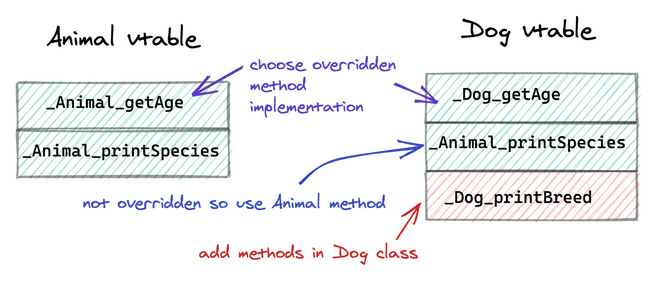
\includegraphics[width=\linewidth]{11_files/vtable.png}

%\hypertarget{series-creating-the-bolt-compiler}{%
%\section{Series: Creating the Bolt
%Compiler}\label{series-creating-the-bolt-compiler}}
%
%\begin{itemize}
%\item
%  { Part 1:
%  }\href{https://mukulrathi.com/create-your-own-programming-language/intro-to-compiler/}{How
%  I wrote my own "proper" programming language}
%\item
%  { Part 2:
%  }\href{https://mukulrathi.com/create-your-own-programming-language/compiler-engineering-structure/}{So
%  how do you structure a compiler project?}
%\item
%  { Part 3:
%  }\href{https://mukulrathi.com/create-your-own-programming-language/parsing-ocamllex-menhir/}{Writing
%  a Lexer and Parser using OCamllex and Menhir}
%\item
%  { Part 4:
%  }\href{https://mukulrathi.com/create-your-own-programming-language/intro-to-type-checking/}{An
%  accessible introduction to type theory and implementing a
%  type-checker}
%\item
%  { Part 5:
%  }\href{https://mukulrathi.com/create-your-own-programming-language/data-race-dataflow-analysis/}{A
%  tutorial on liveness and alias dataflow analysis}
%\item
%  { Part 6:
%  }\href{https://mukulrathi.com/create-your-own-programming-language/lower-language-constructs-to-llvm/}{Desugaring
%  - taking our high-level language and simplifying it!}
%\item
%  { Part 7:
%  }\href{https://mukulrathi.com/create-your-own-programming-language/protobuf-ocaml-cpp-tutorial/}{A
%  Protobuf tutorial for OCaml and C++}
%\item
%  { Part 8:
%  }\href{https://mukulrathi.com/create-your-own-programming-language/llvm-ir-cpp-api-tutorial/}{A
%  Complete Guide to LLVM for Programming Language Creators}
%\item
%  { Part 9:
%  }\href{https://mukulrathi.com/create-your-own-programming-language/concurrency-runtime-language-tutorial/}{Implementing
%  Concurrency and our Runtime Library}
%\item
%  { Part 10:
%  }\href{https://mukulrathi.com/create-your-own-programming-language/generics-parametric-polymorphism/}{Generics
%  - adding polymorphism to Bolt}
%\item
%  \textbf{Part 11: Adding Inheritance and Method Overriding to Our
%  Language}
%\end{itemize}
%
%\begin{center}\rule{0.5\linewidth}{0.5pt}\end{center}

Welcome back to part 11 of the series! We've got concurrency and
generics in our language, but we're still missing a key component:
\textbf{inheritance}. Remember, the four main OOP principles are

\begin{itemize}
\tightlist
\item
  Abstraction
\item
  Encapsulation
\item
  Inheritance
\item
  Polymorphism
\end{itemize}

Ah yes, there's polymorphism to tackle too. We've seen \emph{ad-hoc}
polymorphism, when we implemented
\href{https://mukulrathi.com/create-your-own-programming-language/lower-language-constructs-to-llvm/}{method
overloading in the desugaring stage}. We've seen \emph{parameteric}
polymorphism, when we implemented
\href{https://mukulrathi.com/create-your-own-programming-language/generics-parametric-polymorphism/}{generics}
last time round. In this post we'll cover the
\href{https://en.wikipedia.org/wiki/Polymorphism_(computer_science)}{third
type of polymorphism}: subtype polymorphism - \textbf{method
overriding}.

By the end of the tutorial, we'll be able to compile the following
program. We'll refer to this example to \emph{motivate} the changes
needed to the compiler, so that not only will you understand how the
changes work, but you'll understand \emph{why} they are implemented in
that way.

And hopefully, you'll be able to see the general principles we've used
to add generics in the last post, and inheritance and method overriding
in this post, so you'll be able to add even more language features going
forward!

%Copy

\begin{verbatim}
class Breed {...}
class Species { ... }
class Animal {  
   int age;  
   Species species;  
   int getAge() {    return this.age  }  
   void printSpecies(){ ... }
}

class Dog extends Animal {  
    Breed breed;  
    int getAge() {    return 7*this.age // dog years!  }  
    void printBreed(){ ... }
}

function void printAge(Animal a){  
   printf("I'm %d years old!", a.getAge());
}
void main() {  
  let animal = new Animal(age: 2);  
  let dog = new Dog(age: 2);
  printAge(animal) // print 2  
  printAge(dog) // print 14
}
\end{verbatim}

\hypertarget{just-give-me-the-code}{%
\section{\texorpdfstring{\protect\hyperlink{just-give-me-the-code}{}Just
give me the
code!}{Just give me the code!}}\label{just-give-me-the-code}}

As with the rest of the series, all the code can be found in the
\href{https://github.com/mukul-rathi/bolt}{Bolt repository}.

If you want to see the specific commits that were needed to implement
inheritance, check out
\href{https://github.com/mukul-rathi/bolt/pull/133}{this pull request}
and \href{https://github.com/mukul-rathi/bolt/pull/136}{this pull
request}.

\hypertarget{ast-definitions}{%
\section{\texorpdfstring{\protect\hyperlink{ast-definitions}{}AST
definitions}{AST definitions}}\label{ast-definitions}}

We need to store this inheritance relationship in our Abstract Syntax
Tree for our compiler to access. The easiest way is to store the name of
the superclass in the class definition, since we're reading it in when
we parse \texttt{CLASS\ Someclass\ EXTENDS\ Otherclass}:

%{
%\href{https://github.com/mukul-rathi/bolt/blob/master/src/frontend/parsing/parsed_ast.mli}{parsed\_ast.mli}}
%
%Copy

\begin{lstlisting}[language=caml,caption={parsed\_ast.mli}]
type class_defn = TClass of      Class_name.t      * generic_type option      * Class_name.t option (* optional superclass *)      * capability list      * field_defn list      * method_defn list
\end{lstlisting}

\hypertarget{type-checker}{%
\section{\texorpdfstring{\protect\hyperlink{type-checker}{}Type-Checker}{Type-Checker}}\label{type-checker}}

When we're adding a new language feature, we need to determine what
effect it has on the existing typing rules. With inheritance and method
overriding we have the following new rules:

\begin{itemize}
\tightlist
\item
  Subclasses like \texttt{Dog} have access to not only their own fields
  and methods, but also their superclass \texttt{Animal}'s fields and
  methods, (and the fields and methods of their superclass' superclass,
  and so on up the inheritance hierarchy).
\item
  Overridden methods (\texttt{getAge}) need to have the same type
  signature as their superclass (their return types need to match),
  since they're being used in the same contexts.
\item
  If a superclass is generic, then the subclass must also be generic -
  otherwise how could it access a field of generic type \texttt{T} in
  the superclass?
\item
  Subclasses like \texttt{Dog} are \textbf{subtypes} of their superclass
  (\texttt{Animal}). We have some new typing rules to handle when you
  can use \texttt{Dog} in place of \texttt{Animal}.
\end{itemize}

\hypertarget{accessing-superclass-methods}{%
\subsection{\texorpdfstring{\protect\hyperlink{accessing-superclass-methods}{}Accessing
superclass'
methods}{Accessing superclass' methods}}\label{accessing-superclass-methods}}

We just need to update the \texttt{get\_class\_methods},
\texttt{get\_class\_fields}, methods etc. to recursively look up the
method/field first in the current class, then its superclass and so on.

Here's a simple example: each class has a list of capabilities. With
inheritance, we do a recursive check to get the superclass' capabilities
too. The other \texttt{get\_class\_} methods are similar:

%{
%\href{https://github.com/mukul-rathi/bolt/blob/master/src/frontend/typing/type_env.ml\#L103-L125}{type\_env.ml}}
%
%Copy

\begin{lstlisting}[language=caml,caption={type\_env.ml}]
let rec get_class_capabilities class_name class_defns =  let open Result in  get_class_defn class_name class_defns Lexing.dummy_pos  >>= fun (Parsed_ast.TClass (_, _, maybe_superclass, capabilities, _, _)) ->  ( match maybe_superclass with  | Some superclass -> get_class_capabilities superclass class_defns  | None             -> Ok [] )  >>| fun superclass_caps -> List.concat [superclass_caps; capabilities]
\end{lstlisting}

\hypertarget{generics-and-inheritance}{%
\subsection{\texorpdfstring{\protect\hyperlink{generics-and-inheritance}{}Generics
and
Inheritance}{Generics and Inheritance}}\label{generics-and-inheritance}}

We pattern-match - if the current class isn't generic, and the
superclass is generic, raise a type error!

%{
%\href{https://github.com/mukul-rathi/bolt/blob/master/src/frontend/typing/type_env.type_inheritance\#L37-L47}{type\_inheritance.ml}}
%
%Copy

\begin{lstlisting}[language=caml,caption={type\_inheritance.ml}]
let type_generics_inheritance class_name curr_class_maybe_generic    (Parsed_ast.TClass (superclass_name, superclass_maybe_generic, _, _, _, _)) =  match (curr_class_maybe_generic, superclass_maybe_generic) with  | None, None | Some Generic, None | Some Generic, Some Generic -> Ok ()  | None, Some Generic ->      Error        (Error.of_string           (Fmt.str              "Type error: class %s must be generic since superclass %s is generic@."              (Class_name.to_string class_name)              (Class_name.to_string superclass_name)))
\end{lstlisting}

\hypertarget{method-overriding}{%
\subsection{\texorpdfstring{\protect\hyperlink{method-overriding}{}Method
overriding}{Method overriding}}\label{method-overriding}}

Remember, a method \emph{overrides} another if it has the same name and
parameter types (as \texttt{getAge} does in our example). To check the
overriding methods have the right type, we look up the method type
signatures of the current class and the superclass' methods. We raise an
error if the current class has a method that overrides an inherited
method (same method name and parameter types) but differs in return
type.

%{
%\href{https://github.com/mukul-rathi/bolt/blob/master/src/frontend/typing/type_env.type_inheritance\#L55-L79}{type\_inheritance.ml}}
%
%Copy

\begin{lstlisting}[caption={type\_inheritance.ml},language=caml]
let type_method_overriding class_name class_defns method_defns superclass_defn =  let open Result in  get_methods_type_sigs method_defns  |> fun methods_type_sigs ->  get_methods_type_sigs  (get_class_methods class_defns superclass_defn None Lexing.dummy_pos)  |> fun inherited_methods_type_sigs ->  List.filter    ~f:(fun (meth_name, ret_type, param_types) ->      List.exists        ~f:(fun (inherited_meth_name, inherited_ret_type, inherited_param_types) ->          meth_name = inherited_meth_name          && param_types = inherited_param_types          && not (ret_type = inherited_ret_type))        inherited_methods_type_sigs)    methods_type_sigs  |> function  (* we find any methods that violate overriding types *)  | []                     -> Ok ()  (* no violating methods *)  | (meth_name, _, _) :: _ ->      Error ...
\end{lstlisting}

\hypertarget{subtyping}{%
\subsection{\texorpdfstring{\protect\hyperlink{subtyping}{}Subtyping}{Subtyping}}\label{subtyping}}

We say a type \texttt{A} \emph{subtypes} type \texttt{B}, if we can use
\texttt{A} \textbf{in place of} \texttt{B}. That occurs if they're equal
(obvious) or if \texttt{A} is a subclass of \texttt{B} e.g. \texttt{Dog}
in place of \texttt{Animal}. Equivalently, we can say B is the
\emph{supertype} of A.

{
\href{https://github.com/mukul-rathi/bolt/blob/master/src/frontend/typing/type_env.type_inheritance\#L14-L20}{type\_inheritance.ml}}

Copy

\begin{lstlisting}[caption={type\_inheritance.ml},language=caml]
let is_subtype_of class_defns type_1 type_2 =  type_1 = type_2  ||  match (type_1, type_2) with  | TEClass (class_1, type_param_1), TEClass (class_2, type_param_2) ->      type_param_1 = type_param_2 && is_subclass_of class_defns class_1 class_2  | _ -> false
\end{lstlisting}

Intuitively the subtype, \texttt{A}, has \textbf{more info} than
\texttt{B}: the \texttt{Dog} class has all the \texttt{Animal} behaviour
and then some more behaviour specific to dogs.

When do we use subtyping?

\hypertarget{subtyping-in-variable-assignments}{%
\paragraph{\texorpdfstring{\protect\hyperlink{subtyping-in-variable-assignments}{}Subtyping
in Variable
Assignments}{Subtyping in Variable Assignments}}\label{subtyping-in-variable-assignments}}

We can assign subtypes to variables e.g.
\texttt{let\ x:\ Animal\ =\ new\ Dog()}. So in our \texttt{let}
expression typing judgement, we ensure the bound expr is a subtype of
the type annotation:

%{
%\href{https://github.com/mukul-rathi/bolt/blob/master/src/frontend/typing/type_expr.ml\#L88}{type\_inheritance.ml}}
%
%Copy


\begin{lstlisting}[caption={type\_inheritance.ml},language=caml]
| Parsed_ast.Let (loc, maybe_type_annot, var_name, bound_expr) ->      ...      type_with_defns bound_expr env      >>= fun (typed_bound_expr, bound_expr_type) ->        ( match maybe_type_annot with      | Some type_annot ->          if is_subtype_of class_defns bound_expr_type type_annot then Ok type_annot      ...
\end{lstlisting}

\hypertarget{subtyping-in-functions}{%
\paragraph{\texorpdfstring{\protect\hyperlink{subtyping-in-functions}{}Subtyping
in Functions}{Subtyping in Functions}}\label{subtyping-in-functions}}

Subtyping rules for functions are a little more complicated, so we'll
use our intuitive notion of subtypes having more info to help us out
here.

We can pass subtypes as arguments, as if the function \texttt{printAge}
was expecting an \texttt{Animal} and we give it a \texttt{Dog}, it can
ignore the extra info like \texttt{breed}. Here's the snippet of code
that does the check:

%{
%\href{https://github.com/mukul-rathi/bolt/blob/5543a135edc67bd8054141cbf99d68c44df59fb9/src/frontend/typing/type_overloading.ml\#L79-L80}{type\_overloading.ml}}
%
%Copy


\begin{lstlisting}[caption={type\_overloading.ml},language=caml]
...if are_subtypes_of class_defns args_types param_types then        Ok (param_types, return_type)...
\end{lstlisting}

Hold on, you ask, why is this subtype check in the
\texttt{type\_overloading} file?

Well, as you add language features, they start to interact with each
other.
\href{https://mukulrathi.com/create-your-own-programming-language/lower-language-constructs-to-llvm/}{Earlier
in the series}, we added function overloading: i.e. multiple functions
with the same name but different parameter types. We choose the correct
overloaded function based on the argument types: we pick the function
whose parameter types \emph{match}. Before, our definition of
\emph{match} was that the types were equal. Now, we say they
\emph{match} if the argument types are \textbf{subtypes} of the param
types.
\href{https://github.com/mukul-rathi/bolt/blob/master/src/frontend/typing/type_overloading.ml\#L89}{All
the details are in the code}.

Likewise, when type-checking our function return type, the body type
\emph{matches} the function return type, if it is a subtype. (If the
function returns \texttt{void} we don't care about the body type.)

%{
%\href{https://github.com/mukul-rathi/bolt/blob/master/src/frontend/typing/type_functions.ml\#L43}{type\_functions.ml}}
%
%Copy

\begin{lstlisting}[language=caml,caption={type\_functions.ml}]
...>>= fun (typed_body_expr, body_return_type) -> if return_type = TEVoid || is_subtype_of class_defns body_return_type return_type then    Ok ...else Error ...
\end{lstlisting}

An identical check is done to
\href{https://github.com/mukul-rathi/bolt/blob/master/src/frontend/typing/type_classes.ml\#L84}{type-check
methods}.

\hypertarget{lowering-to-llvm}{%
\section{\texorpdfstring{\protect\hyperlink{lowering-to-llvm}{}Lowering
to LLVM}{Lowering to LLVM}}\label{lowering-to-llvm}}

Now we've done the type-checking, we need to output LLVM IR in order to
run the program. Let's quickly remind ourselves of the program we're
trying to compile:

Copy

\begin{verbatim}
class Animal {  
  int age;  
  Species species;  
 int getAge() {    return this.age  } 
   void printSpecies(){ ... }
}

class Dog extends Animal {  
  Breed breed;  
  int getAge() {    return 7*this.age // dog years!  }  
  void printBreed(){ ... }
}

function void printAge(Animal a){  
   printf("I'm %d years old!", a.getAge());
}
void main() {
  let animal = new Animal(age: 2);
  let dog = new Dog(age: 2);
  printAge(animal) // print 2
  printAge(dog) // print 14
}
\end{verbatim}

\hypertarget{inheritance-and-structs}{%
\subsection{\texorpdfstring{\protect\hyperlink{inheritance-and-structs}{}Inheritance
and Structs}{Inheritance and Structs}}\label{inheritance-and-structs}}

Both the \texttt{Animal}and \texttt{Dog} classes are desugared to
structs containing their fields. This desugaring is straightforward for
\texttt{Animal}:

Copy

\begin{verbatim}
struct Animal {  int age;  Species *species;}
\end{verbatim}

Accessing the \texttt{age} field is desugared into getting a pointer to
field \texttt{0} of the struct, and likewise \texttt{species} is field
\texttt{1}.

On to the struct for \texttt{Dog}. We have three requirements:

\begin{itemize}
\tightlist
\item
  The struct needs to contain the fields in the \texttt{Dog} class.
\item
  It also needs to contain the fields in the \texttt{Animal} class.
\item
  A \texttt{Dog} struct should be able to be used wherever an
  \texttt{Animal} struct is expected.
\end{itemize}

The last point is the critical one. Say I have a \texttt{dog} object
being treated as an \texttt{Animal}. When I query \texttt{dog.age} and
\texttt{dog.species}, I'll expect them to be in field \texttt{0} and
\texttt{1} of the struct, since it's of type \texttt{Animal}. So the
\texttt{Dog} struct needs to preserve that field indexing. So the only
place the field \texttt{breed} can go is at index \texttt{2}.

Copy

\begin{verbatim}
struct Dog {  int age;  Species *species;  Breed *breed;}
\end{verbatim}

{
\href{https://mukulrathi.com/static/a759ba239e743d4372cd86fb6e9bc856/8affb/inheritance-struct.png}{{}
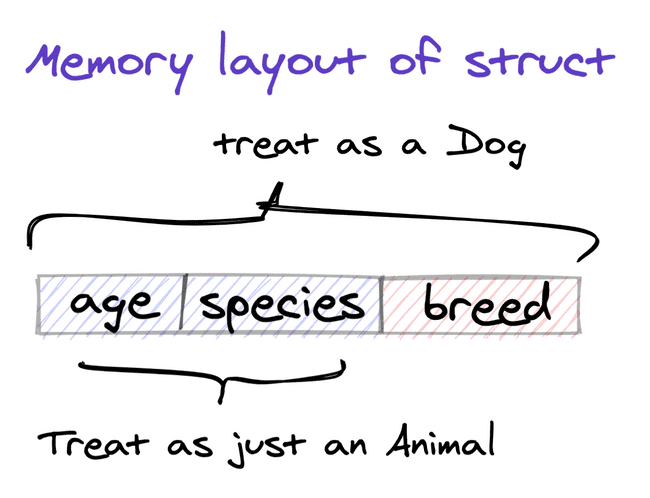
\includegraphics[width=\linewidth]{11_files/inheritance-struct.png}} }

In general, we order the struct so all the superclass's fields go first,
\emph{then} any fields declared in the current class. If we added a
subclass \texttt{Labrador}:

%Copy

\begin{verbatim}
class Labrador extends Dog{  Colour colour;}
// Desugared
struct Labrador {
  int age;
  Species *species;
  Breed *breed;
  Colour *colour;
}
\end{verbatim}

{
\href{https://mukulrathi.com/static/2ee5657d689e2e35a975960beace0cbb/a9577/another-inheritance-struct.png}{{}
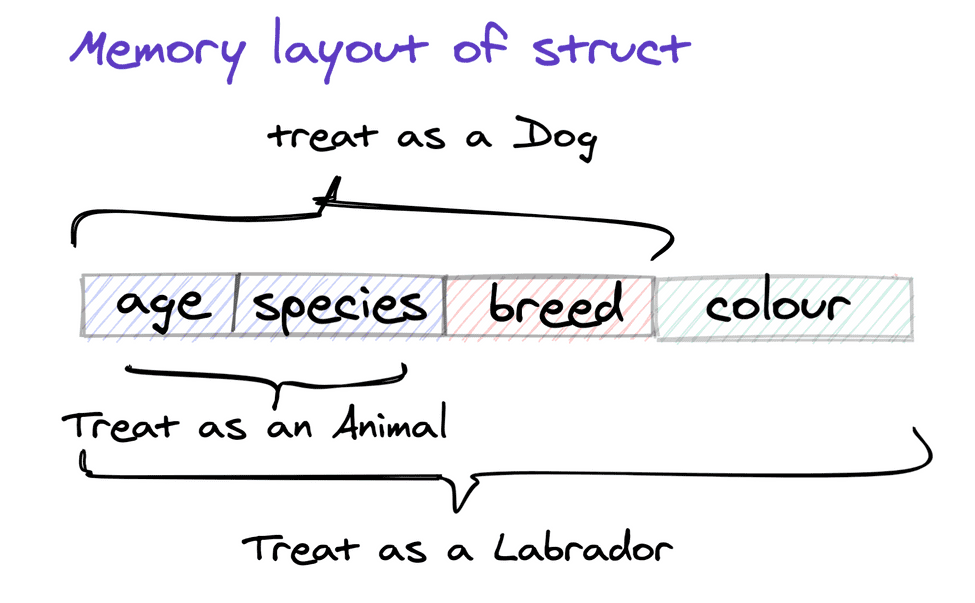
\includegraphics[width=\linewidth]{11_files/another-inheritance-struct.png}} }

If we want to treat a \texttt{Labrador} as an \texttt{Animal}, only look
at the first 2 fields. If you want to treat it as a \texttt{Dog} look at
the first 3 fields. And so on.

You can see this ordering in our \texttt{get\_class\_fields} method
during our IR generation stage, which puts \texttt{superclass\_fields}
first.

%{
%\href{https://github.com/mukul-rathi/bolt/blob/master/src/frontend/ir_gen/ir_gen_env.ml\#L17}{ir\_gen\_env.ml}}
%
%Copy

\begin{lstlisting}[language=caml,caption={ir\_gen\_env.ml}]
let rec get_class_fields class_name class_defns =  get_class_defn class_name class_defns  |> fun (TClass (_, maybe_superclass, _, fields, _)) ->  ( match maybe_superclass with  | Some super_class -> get_class_fields super_class class_defns  | None             -> [] )  |> fun superclass_fields -> List.concat [superclass_fields; fields]
\end{lstlisting}

Since we've handled this in the Bolt IR gen stage of the compiler
frontend, we don't need to change our LLVM backend, right?

Almost right. Just one hitch: LLVM IR is \textbf{typed}, so it will
complain if we pass a \texttt{Dog\ *} pointer to a function that expects
a \texttt{Animal\ *} pointer. Remember, LLVM has no notion of
inheritance, just raw structs, so it can't see that \texttt{Dog} is a
subclass of \texttt{Animal}. We thus \emph{explicitly cast} the argument
pointer to the function's expected param type before we pass it to the
function:

%{
%\href{https://github.com/mukul-rathi/bolt/blob/master/src/llvm-backend/llvm_ir_codegen/expr_codegen.cc\#L181-L191}{expr\_codegen.cc}}
%
%Copy

\begin{lstlisting}[language=C++,caption={expr\_codegen.cc}]
std::vector<Value *> argVals;  
for (int i = 0; i < expr.arguments.size(); i++) {
    Value *argVal = expr.arguments[i]->codegen(*this);
    Type *paramTy = calleeFunTy->getParamType(i);
    Value *bitCastArgVal = builder->CreateBitCast(argVal, paramTy);
    argVals.push_back(bitCastArgVal);  
}
\end{lstlisting}

\hypertarget{method-overriding-and-virtual-tables}{%
\subsection{\texorpdfstring{\protect\hyperlink{method-overriding-and-virtual-tables}{}Method
Overriding and Virtual
Tables}{Method Overriding and Virtual Tables}}\label{method-overriding-and-virtual-tables}}

Method overriding is a bit tricky, so take a breather.
\href{http://mukulrathi.co.uk/create-your-own-programming-language/lower-language-constructs-to-llvm/\#lowering-objects-to-structs}{From
our previous post}, we have that methods are desugared to regular
functions:

\begin{figure}
\centering
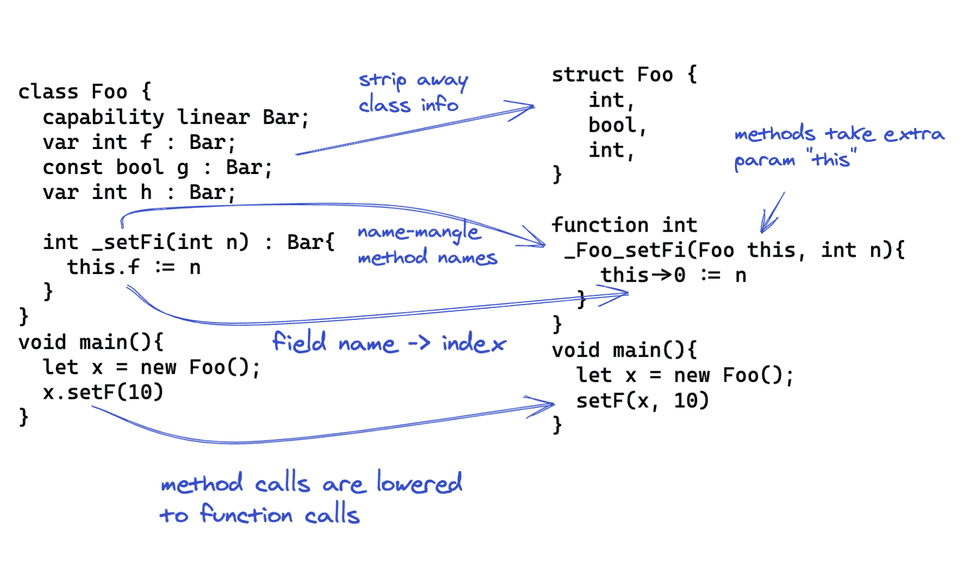
\includegraphics[width=\linewidth]{11_files/lower-classes.png}
\caption{The diagram from our previous desugaring post.}
\end{figure}

In our running example in this post we have \texttt{getAge} overridden,
so we have these two functions corresponding to the implementation of
\texttt{getAge} in each of the classes:

%Copy

\begin{verbatim}
Animal_getAge(Animal this){  return this.age}
Dog_getAge(Dog this){  return 7 * this.age}
\end{verbatim}

When we call \texttt{a.age()} in our \texttt{printAge} function, we want
to call \texttt{Animal\_getAge} if the underlying object is an
\texttt{Animal}, and \texttt{Dog\_getAge} if the object is actually a
\texttt{Dog}. The thing is, in general we don't know this information at
compile-time. Here's an example where type of \texttt{dog} is only known
at runtime:

%Copy

\begin{verbatim}
let dog = new Animal()
if (someCondition) {
  dog = new Dog()
}
dog.getAge() // which function do we call?
\end{verbatim}

So how do we insert the right call? The problem is not too dissimilar to
this:

%Copy

\begin{verbatim}
let dog = new Animal()
dog.age = 7
if (someCondition) {
  dog.age = 14
}
dog.age // which value does age have?
\end{verbatim}

We know how to do this: look up the value by indexing into the
\emph{list of fields} in the \texttt{dog} struct at runtime (index
\texttt{0} for \texttt{age}).

Since we've solved the problem for fields, let's do the same thing for
methods. We can create a \emph{list of (pointers to) methods} for each
class, called the \textbf{virtual table} or \textbf{vtable}. Instead of
determining the function call at compile-time, we instead provide an
\emph{index} into the table and call the function pointed to at that
index at runtime.

For similar reasons to the struct fields before, superclasses' methods
come before the current class's methods in the vtable. So we have
\texttt{getAge}, \texttt{printSpecies} first as they're from
\texttt{Animal}, then we have \texttt{getBreed} from \texttt{Dog}. To
override a method, we just replace its entry in the table:

{
\href{https://mukulrathi.com/static/c32dbd45d3466359a751c298568c0f5f/bfe41/vtable.png}{{}
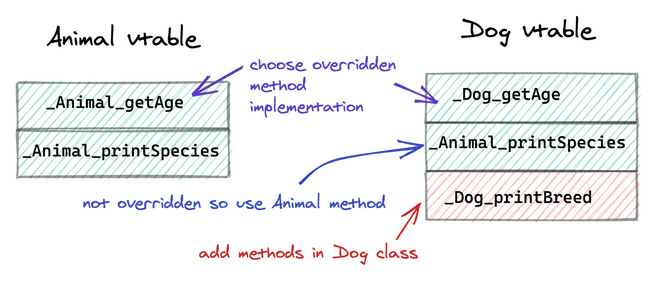
\includegraphics[width=\linewidth]{11_files/vtable.png}} }

Now we can just say for \texttt{dog.getAge()}, look at index \texttt{0}
of the \texttt{dog}'s vtable, and execute whichever function's there. Or
index \texttt{1} for \texttt{dog.printSpecies()}. \textbf{Problem
solved!}

\hypertarget{virtual-tables-in-our-structs}{%
\paragraph{\texorpdfstring{\protect\hyperlink{virtual-tables-in-our-structs}{}Virtual
Tables in our
structs}{Virtual Tables in our structs}}\label{virtual-tables-in-our-structs}}

Unlike fields, which are different for each object, vtables are the same
for \emph{all} objects of a \emph{given class}. Having a copy of the
same vtable in each object is wasteful: instead have just \textbf{one}
global vtable \textbf{per class}, and have the objects store a
\emph{pointer} to that.

We've reserved the first field in our object struct for the vtable
pointer:

%Copy

\begin{verbatim}
struct Animal {
  AnimalVTable *vtableptr;
  int age;
  Species *species;
}
struct Dog {
  DogVTable *vtableptr;
  int age;
  Species *species;
  Breed *breed;
}
\end{verbatim}

Okay, let's implement it with some code! To generate the vtable, we get
a list of the class' methods, \textbf{annotated} with the class they
came from (so we get the right overridden method). That is, we don't
have \texttt{getAge} we have the pair \texttt{(Dog,\ getAge)}. We use
this pair to generate the name-mangled function name:
\texttt{\_Dog\_getAge}. Our vtable is just a list of these name-mangled
function names.

%{
%\href{https://github.com/mukul-rathi/bolt/blob/master/src/frontend/ir_gen/ir_gen_env.ml\#L65-L70}{ir\_gen\_env.ml}}
%
%Copy

\begin{lstlisting}[language=caml,caption={ir\_gen\_env.ml}]
let ir_gen_vtable class_name class_defns =  get_class_annotated_methods class_name class_defns  |> fun class_annotated_methods ->  List.map    ~f:(fun (class_annot, meth_name) -> name_mangle_method_name meth_name class_annot)    class_annotated_methods
\end{lstlisting}

\hypertarget{llvm-implementation-of-virtual-tables}{%
\paragraph{\texorpdfstring{\protect\hyperlink{llvm-implementation-of-virtual-tables}{}LLVM
implementation of Virtual
Tables}{LLVM implementation of Virtual Tables}}\label{llvm-implementation-of-virtual-tables}}

We implement VTables as a struct of function pointers. Below are the
type definitions, and the corresponding global variable declaration.

%{
%\href{https://github.com/mukul-rathi/bolt/blob/master/tests/e2e/vtable.ll.expected}{vtable.ll}}
%
%Copy

\begin{lstlisting}[language=llvm,caption={vtable.ll}]
%_VtableAnimal = type { i32 (%Animal*)*, void (%Animal*)* }
%_VtableDog = type { i32 (%Dog*)*, void (%Animal*)*, void (%Dog*)*}
@_VtableAnimal = global %_VtableAnimal { i32 (%Animal*)* @_Animal__getAge, void (%Animal*)* @_Animal__printSpecies }
@_VtableDog = global %_VtableDog { i32 (%Dog*)* @_Dog__getAge, void (%Animal*)* @_Animal__printSpecies, void (%Dog*)* @_Dog__printBreed }
%Animal = type { %_VtableAnimal*, i8*, i32, i32, i32, %Species* }
%Dog = type { %_VtableDog*, %Species*, %Breed* }
\end{lstlisting}

Creating the global vtables follows the format we mentioned
\href{https://mukulrathi.com/create-your-own-programming-language/llvm-ir-cpp-api-tutorial/\#global-variables}{for
global variables in the LLVM post}. We create the table as a
\texttt{ConstantStruct}, and populate the
(\texttt{vector\textless{}Constant\ *\textgreater{}}) body with
\texttt{Function\ *} pointers to each of the methods.

%{
%\href{https://github.com/mukul-rathi/bolt/blob/master/src/llvm-backend/llvm_ir_codegen/class_codegen.cc\#L40-L58}{class\_codegen.cc}}
%
%Copy

\begin{lstlisting}[language=C++,caption={class\_codegen.cc}]
void IRCodegenVisitor::codegenVTables(const std::vector<std::unique_ptr<ClassIR>> &classes) {
  for (auto &currClass : classes) {
    std::string vTableName = "_Vtable" + currClass->className;
    StructType *vTableTy = module->getTypeByName(StringRef(vTableName));
    std::vector<Constant *> vTableMethods;
    std::vector<Type *> vTableMethodTys;
    for (auto &methodName : currClass->vtable) {
      Function *method = module->getFunction(        StringRef(methodName));
      vTableMethods.push_back(method);
      vTableMethodTys.push_back(method->getType());
    }
    vTableTy->setBody(vTableMethodTys);
    module->getOrInsertGlobal(vTableName, vTableTy);

    GlobalVariable *vTable = module->getNamedGlobal(vTableName);
    vTable->setInitializer(      ConstantStruct::get(vTableTy, vTableMethods));  
   }
}
\end{lstlisting}

Then to call the function, we're replacing our static function call:

%Copy

\begin{lstlisting}[language=C++]
*calleeMethod =      module->getFunction(expr.methodName);
\end{lstlisting}

with a vtable lookup. This is just two Struct GEP lookups: first we get
the vtable pointer by reading index \texttt{0} of the object, then we
get the method pointer by using the \texttt{methodIndex} into the
vtable. (Again, {check
the LLVM post for a refresher on LLVM}).

%{
%\href{https://github.com/mukul-rathi/bolt/blob/master/src/llvm-backend/llvm_ir_codegen/expr_codegen.cc\#L200-L208}{expr\_codegen.cc}}
%
%Copy

\begin{lstlisting}[caption={expr\_codegen.cc},language=C++]
Value *vTablePtr = builder->CreateLoad(builder->CreateStructGEP(
    thisObj->getType()
        ->getPointerElementType() /* get type of element on heap*/,
    thisObj, 0));Value *calleeMethodPtr =
    builder->CreateStructGEP(vTablePtr->getType()->getPointerElementType(),
                              vTablePtr, expr.methodIndex);
Value *calleeMethod = builder->CreateLoad(calleeMethodPtr);
\end{lstlisting}

An minor detail, why is \texttt{calleeMethod} now of type
\texttt{Value\ *} not \texttt{Function\ *}? I asked the LLVM dev mailing
list this question - it's because \texttt{Function\ *} refers to a
function known at compile-time. Our vtable functions are looked up at
runtime, so aren't of type \texttt{Function\ *}.

\hypertarget{summary}{%
\section{\texorpdfstring{\protect\hyperlink{summary}{}Summary}{Summary}}\label{summary}}

This post on inheritance and method overriding brings to a close the
Bolt compiler series for now. These tutorials cover the general language
features of the Bolt language at the time I submitted my dissertation.

There's always more language features to add, perhaps later down the
line I'll write another tutorial on arrays! In the meantime, I've got a
host of new posts on other content coming this year - 40 new posts
coming in 2021!

%\hypertarget{i-make-content-about-my-software-engineering-journey-curated-in-my-newsletter}{%
%\subsection{I make content about my software engineering journey,
%curated in my
%newsletter!}\label{i-make-content-about-my-software-engineering-journey-curated-in-my-newsletter}}
%
%Tips from my time at Cambridge and Facebook, and early access to
%technical tutorials on machine learning, compilers and beyond.
%
%\href{https://newsletter.mukulrathi.com/}{Check out previous issues!}
%
%Email Address
%
%By subscribing, you agree with Revue's
%\href{https://www.getrevue.co/terms}{Terms of Service} and
%\href{https://www.getrevue.co/privacy}{Privacy Policy}.

%\hypertarget{share-this-on-twitter}{%
%\subsection{Share This On Twitter}\label{share-this-on-twitter}}
%
%If you liked this post, please consider sharing it with your network. If
%you have any questions, tweet away and I'll answer :) I also tweet when
%new posts drop!
%
%\textbf{PS:} I also share helpful tips and links as I'm learning - so
%you get them \textbf{well before} they make their way into a post!
%
%\hypertarget{series-creating-the-bolt-compiler-1}{%
%\section{Series: Creating the Bolt
%Compiler}\label{series-creating-the-bolt-compiler-1}}
%
%\begin{itemize}
%\item
%  { Part 1:
%  }\href{https://mukulrathi.com/create-your-own-programming-language/intro-to-compiler/}{How
%  I wrote my own "proper" programming language}
%\item
%  { Part 2:
%  }\href{https://mukulrathi.com/create-your-own-programming-language/compiler-engineering-structure/}{So
%  how do you structure a compiler project?}
%\item
%  { Part 3:
%  }\href{https://mukulrathi.com/create-your-own-programming-language/parsing-ocamllex-menhir/}{Writing
%  a Lexer and Parser using OCamllex and Menhir}
%\item
%  { Part 4:
%  }\href{https://mukulrathi.com/create-your-own-programming-language/intro-to-type-checking/}{An
%  accessible introduction to type theory and implementing a
%  type-checker}
%\item
%  { Part 5:
%  }\href{https://mukulrathi.com/create-your-own-programming-language/data-race-dataflow-analysis/}{A
%  tutorial on liveness and alias dataflow analysis}
%\item
%  { Part 6:
%  }\href{https://mukulrathi.com/create-your-own-programming-language/lower-language-constructs-to-llvm/}{Desugaring
%  - taking our high-level language and simplifying it!}
%\item
%  { Part 7:
%  }\href{https://mukulrathi.com/create-your-own-programming-language/protobuf-ocaml-cpp-tutorial/}{A
%  Protobuf tutorial for OCaml and C++}
%\item
%  { Part 8:
%  }\href{https://mukulrathi.com/create-your-own-programming-language/llvm-ir-cpp-api-tutorial/}{A
%  Complete Guide to LLVM for Programming Language Creators}
%\item
%  { Part 9:
%  }\href{https://mukulrathi.com/create-your-own-programming-language/concurrency-runtime-language-tutorial/}{Implementing
%  Concurrency and our Runtime Library}
%\item
%  { Part 10:
%  }\href{https://mukulrathi.com/create-your-own-programming-language/generics-parametric-polymorphism/}{Generics
%  - adding polymorphism to Bolt}
%\item
%  \textbf{Part 11: Adding Inheritance and Method Overriding to Our
%  Language}
%\end{itemize}
%
%\begin{itemize}
%\item ~
%  \hypertarget{generics---adding-polymorphism-to-bolt}{%
%  \subsection{\texorpdfstring{\href{https://mukulrathi.com/create-your-own-programming-language/generics-parametric-polymorphism/}{←
%  Generics - adding polymorphism to
%  Bolt}}{← Generics - adding polymorphism to Bolt}}\label{generics---adding-polymorphism-to-bolt}}
%\item ~
%  \hypertarget{ive-started-a-youtube-channel}{%
%  \subsection{\texorpdfstring{\href{https://mukulrathi.com/new-youtube-channel/}{I've
%  Started a YouTube Channel
%  →}}{I've Started a YouTube Channel →}}\label{ive-started-a-youtube-channel}}
%\end{itemize}
%
%\hypertarget{table-of-contents}{%
%\section{Table of Contents}\label{table-of-contents}}
%
%\href{https://mukulrathi.com/create-your-own-programming-language/inheritance-method-overriding-vtable/\#top-of-page}{}
%
%\hypertarget{adding-inheritance-and-method-overriding-to-our-language}{%
%\subsection{Adding Inheritance and Method Overriding to Our
%Language}\label{adding-inheritance-and-method-overriding-to-our-language}}
%
%\begin{itemize}
%\item
%  \href{https://mukulrathi.com/create-your-own-programming-language/inheritance-method-overriding-vtable/\#just-give-me-the-code}{}
%
%  \hypertarget{just-give-me-the-code-1}{%
%  \subsection{Just give me the code!}\label{just-give-me-the-code-1}}
%\item
%  \href{https://mukulrathi.com/create-your-own-programming-language/inheritance-method-overriding-vtable/\#ast-definitions}{}
%
%  \hypertarget{ast-definitions-1}{%
%  \subsection{AST definitions}\label{ast-definitions-1}}
%\item
%  \href{https://mukulrathi.com/create-your-own-programming-language/inheritance-method-overriding-vtable/\#type-checker}{}
%
%  \hypertarget{type-checker-1}{%
%  \subsection{Type-Checker}\label{type-checker-1}}
%
%  \begin{itemize}
%  \item
%    \href{https://mukulrathi.com/create-your-own-programming-language/inheritance-method-overriding-vtable/\#accessing-superclass-methods}{}
%
%    \hypertarget{accessing-superclass-methods-1}{%
%    \subsection{Accessing superclass'
%    methods}\label{accessing-superclass-methods-1}}
%  \item
%    \href{https://mukulrathi.com/create-your-own-programming-language/inheritance-method-overriding-vtable/\#generics-and-inheritance}{}
%
%    \hypertarget{generics-and-inheritance-1}{%
%    \subsection{Generics and
%    Inheritance}\label{generics-and-inheritance-1}}
%  \item
%    \href{https://mukulrathi.com/create-your-own-programming-language/inheritance-method-overriding-vtable/\#method-overriding}{}
%
%    \hypertarget{method-overriding-1}{%
%    \subsection{Method overriding}\label{method-overriding-1}}
%  \item
%    \href{https://mukulrathi.com/create-your-own-programming-language/inheritance-method-overriding-vtable/\#subtyping}{}
%
%    \hypertarget{subtyping-1}{%
%    \subsection{Subtyping}\label{subtyping-1}}
%  \end{itemize}
%\item
%  \href{https://mukulrathi.com/create-your-own-programming-language/inheritance-method-overriding-vtable/\#lowering-to-llvm}{}
%
%  \hypertarget{lowering-to-llvm-1}{%
%  \subsection{Lowering to LLVM}\label{lowering-to-llvm-1}}
%
%  \begin{itemize}
%  \item
%    \href{https://mukulrathi.com/create-your-own-programming-language/inheritance-method-overriding-vtable/\#inheritance-and-structs}{}
%
%    \hypertarget{inheritance-and-structs-1}{%
%    \subsection{Inheritance and
%    Structs}\label{inheritance-and-structs-1}}
%  \item
%    \href{https://mukulrathi.com/create-your-own-programming-language/inheritance-method-overriding-vtable/\#method-overriding-and-virtual-tables}{}
%
%    \hypertarget{method-overriding-and-virtual-tables-1}{%
%    \subsection{Method Overriding and Virtual
%    Tables}\label{method-overriding-and-virtual-tables-1}}
%  \end{itemize}
%\item
%  \href{https://mukulrathi.com/create-your-own-programming-language/inheritance-method-overriding-vtable/\#summary}{}
%
%  \hypertarget{summary-1}{%
%  \subsection{Summary}\label{summary-1}}
%\end{itemize}
%
%© Mukul Rathi 2023
%
%\hypertarget{gatsby-announcer}{}
%Navigated to Adding Inheritance and Method Overriding to Our Language





%\bibliographystyle{plain}
%\bibliography{bibtex_example}

%\printindex

\end{document}
